\subsection{Теория поля}
	
	\subsubsection{Аннотация}

        Курс <<Теория поля>> получил смешанные отзывы. 
        
        Лекции Геца А.В. получили смешанные отзывы. Совет студентов и аспирантов ФРКТ считат полезным донесение развернутых отзывов респондентов до лектора.

        Лекции Фомичева А.В. получили в основном положительные отзывы, однако есть ряд недостатков. Студенты отметили, что темп лекций был высоким из-за чего трудно было понимать материал. Совет студентов и аспирантов ФРКТ просит передать эти сведения лектору.

        Семинаристы Дудченко В.А., Дьяконов Д.В., Фомичев С.В. получили крайне положительные оценки от респондентов. Совет студентов и аспирантов ФРКТ предлагает поощрить перечисленных преподавателей.

        Семинарист Девизорова Ж.А. получила крайне негативные отзывы. Респонденты отметили, что семинарист непонятно объясняет материал, неоднократно не приходила на сдачи, несвоевременно принимала задания, а также неадекватно оценивала знания студентов. Совет студентов и аспирантов ФРКТ рекомендует заменить этого семинариста.

        Семинарист Осипов Д.Л. получил крайне негативные отзывы. Респонденты отметили, что семинарист непонятно объясняет материал, несвоевременно принимал задания, грубил студентам, а также неадекватно оценивал знания студентов. Совет студентов и аспирантов ФРКТ рекомендует заменить этого семинариста.

        Руководствуясь результатами опроса, Совет студентов и аспирантов ФРКТ выдвигает следующие идеи по улучшению данного курса:
        \begin{enumerate}
            \item пересмотреть кандидатуры семинаристов;
            \item уменьшить объём материала, так как многие респонденты отметили, что конец курса было достаточно тяжело освоить из-за огромного количества тем в учебной программе;
            \item установить четкие критерии оценивания, то есть устранить неясность, на что влияет рекомендованная оценка; 
            \item сделать курс факультативным для студентов ФРКТ, так как он не соответствует их профессиональным потребностям.
        \end{enumerate}


	\subsubsection{Общий отзыв студентов о курсе}

		\begin{figure}[H]
			\centering
			\begin{subfigure}[b]{0.45\textwidth}
				\centering
				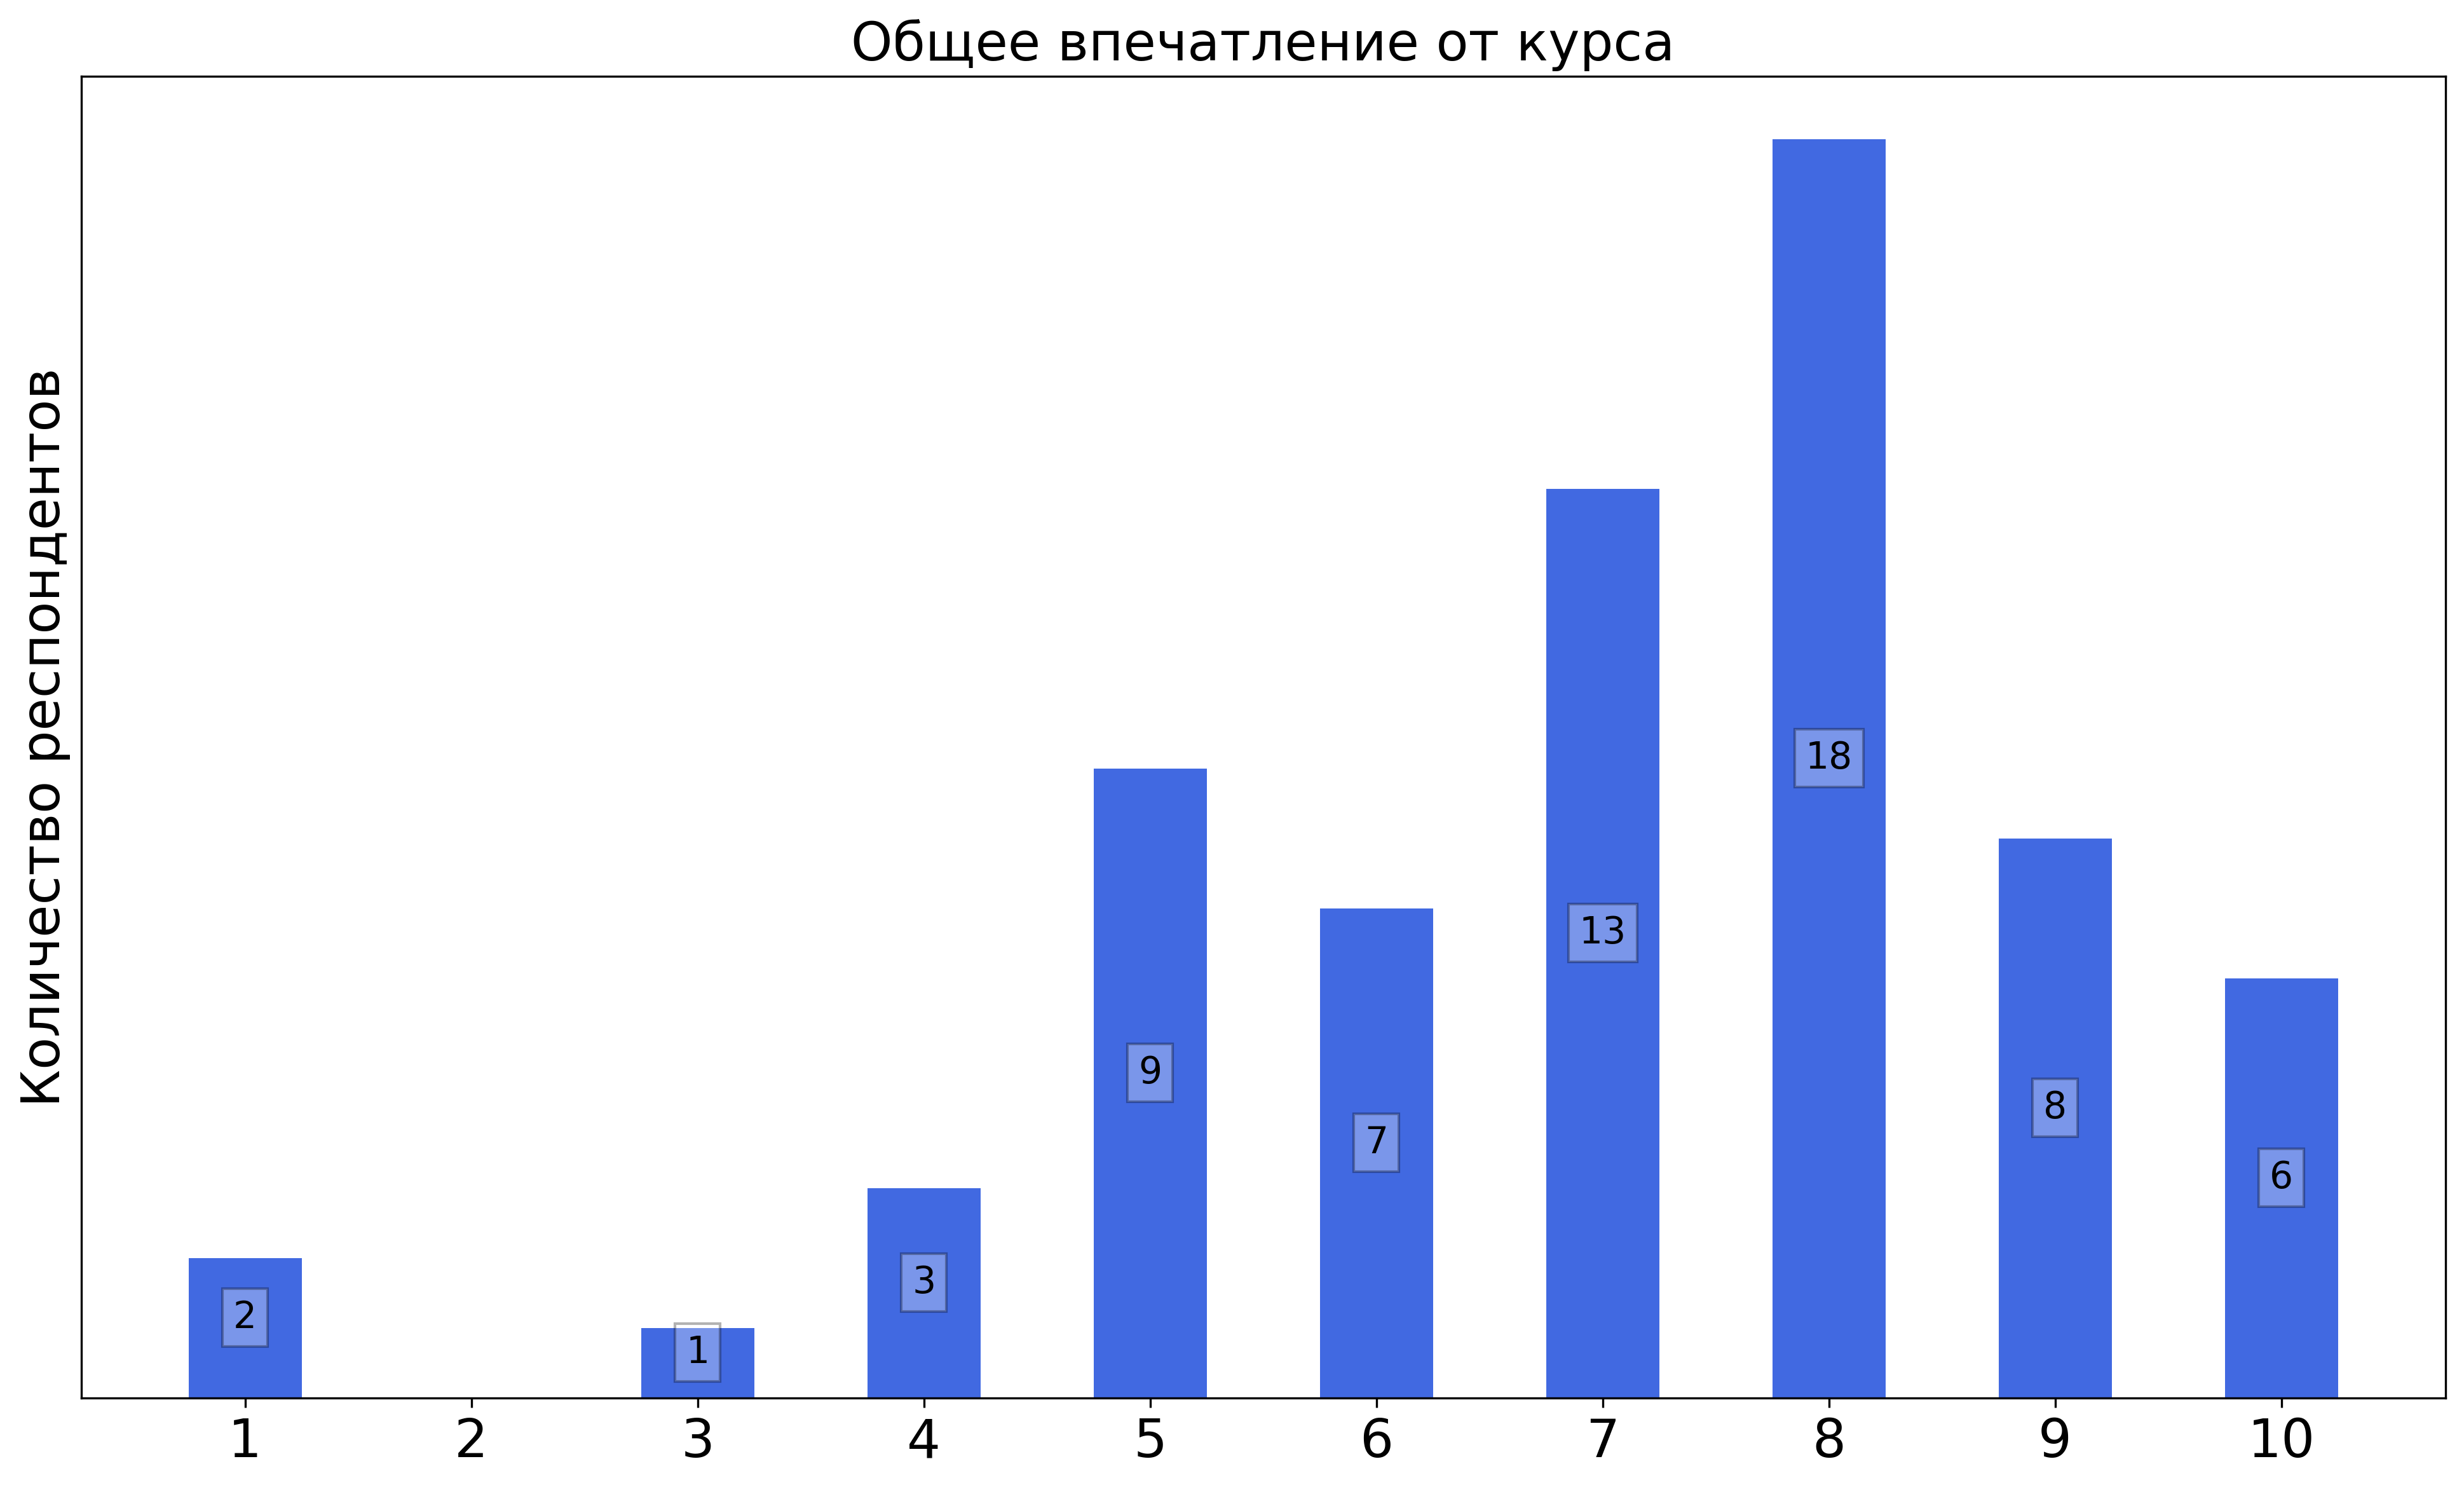
\includegraphics[width=\textwidth]{images/3 course/Теория поля/general-0.png}
			\end{subfigure}
			\begin{subfigure}[b]{0.45\textwidth}
				\centering
				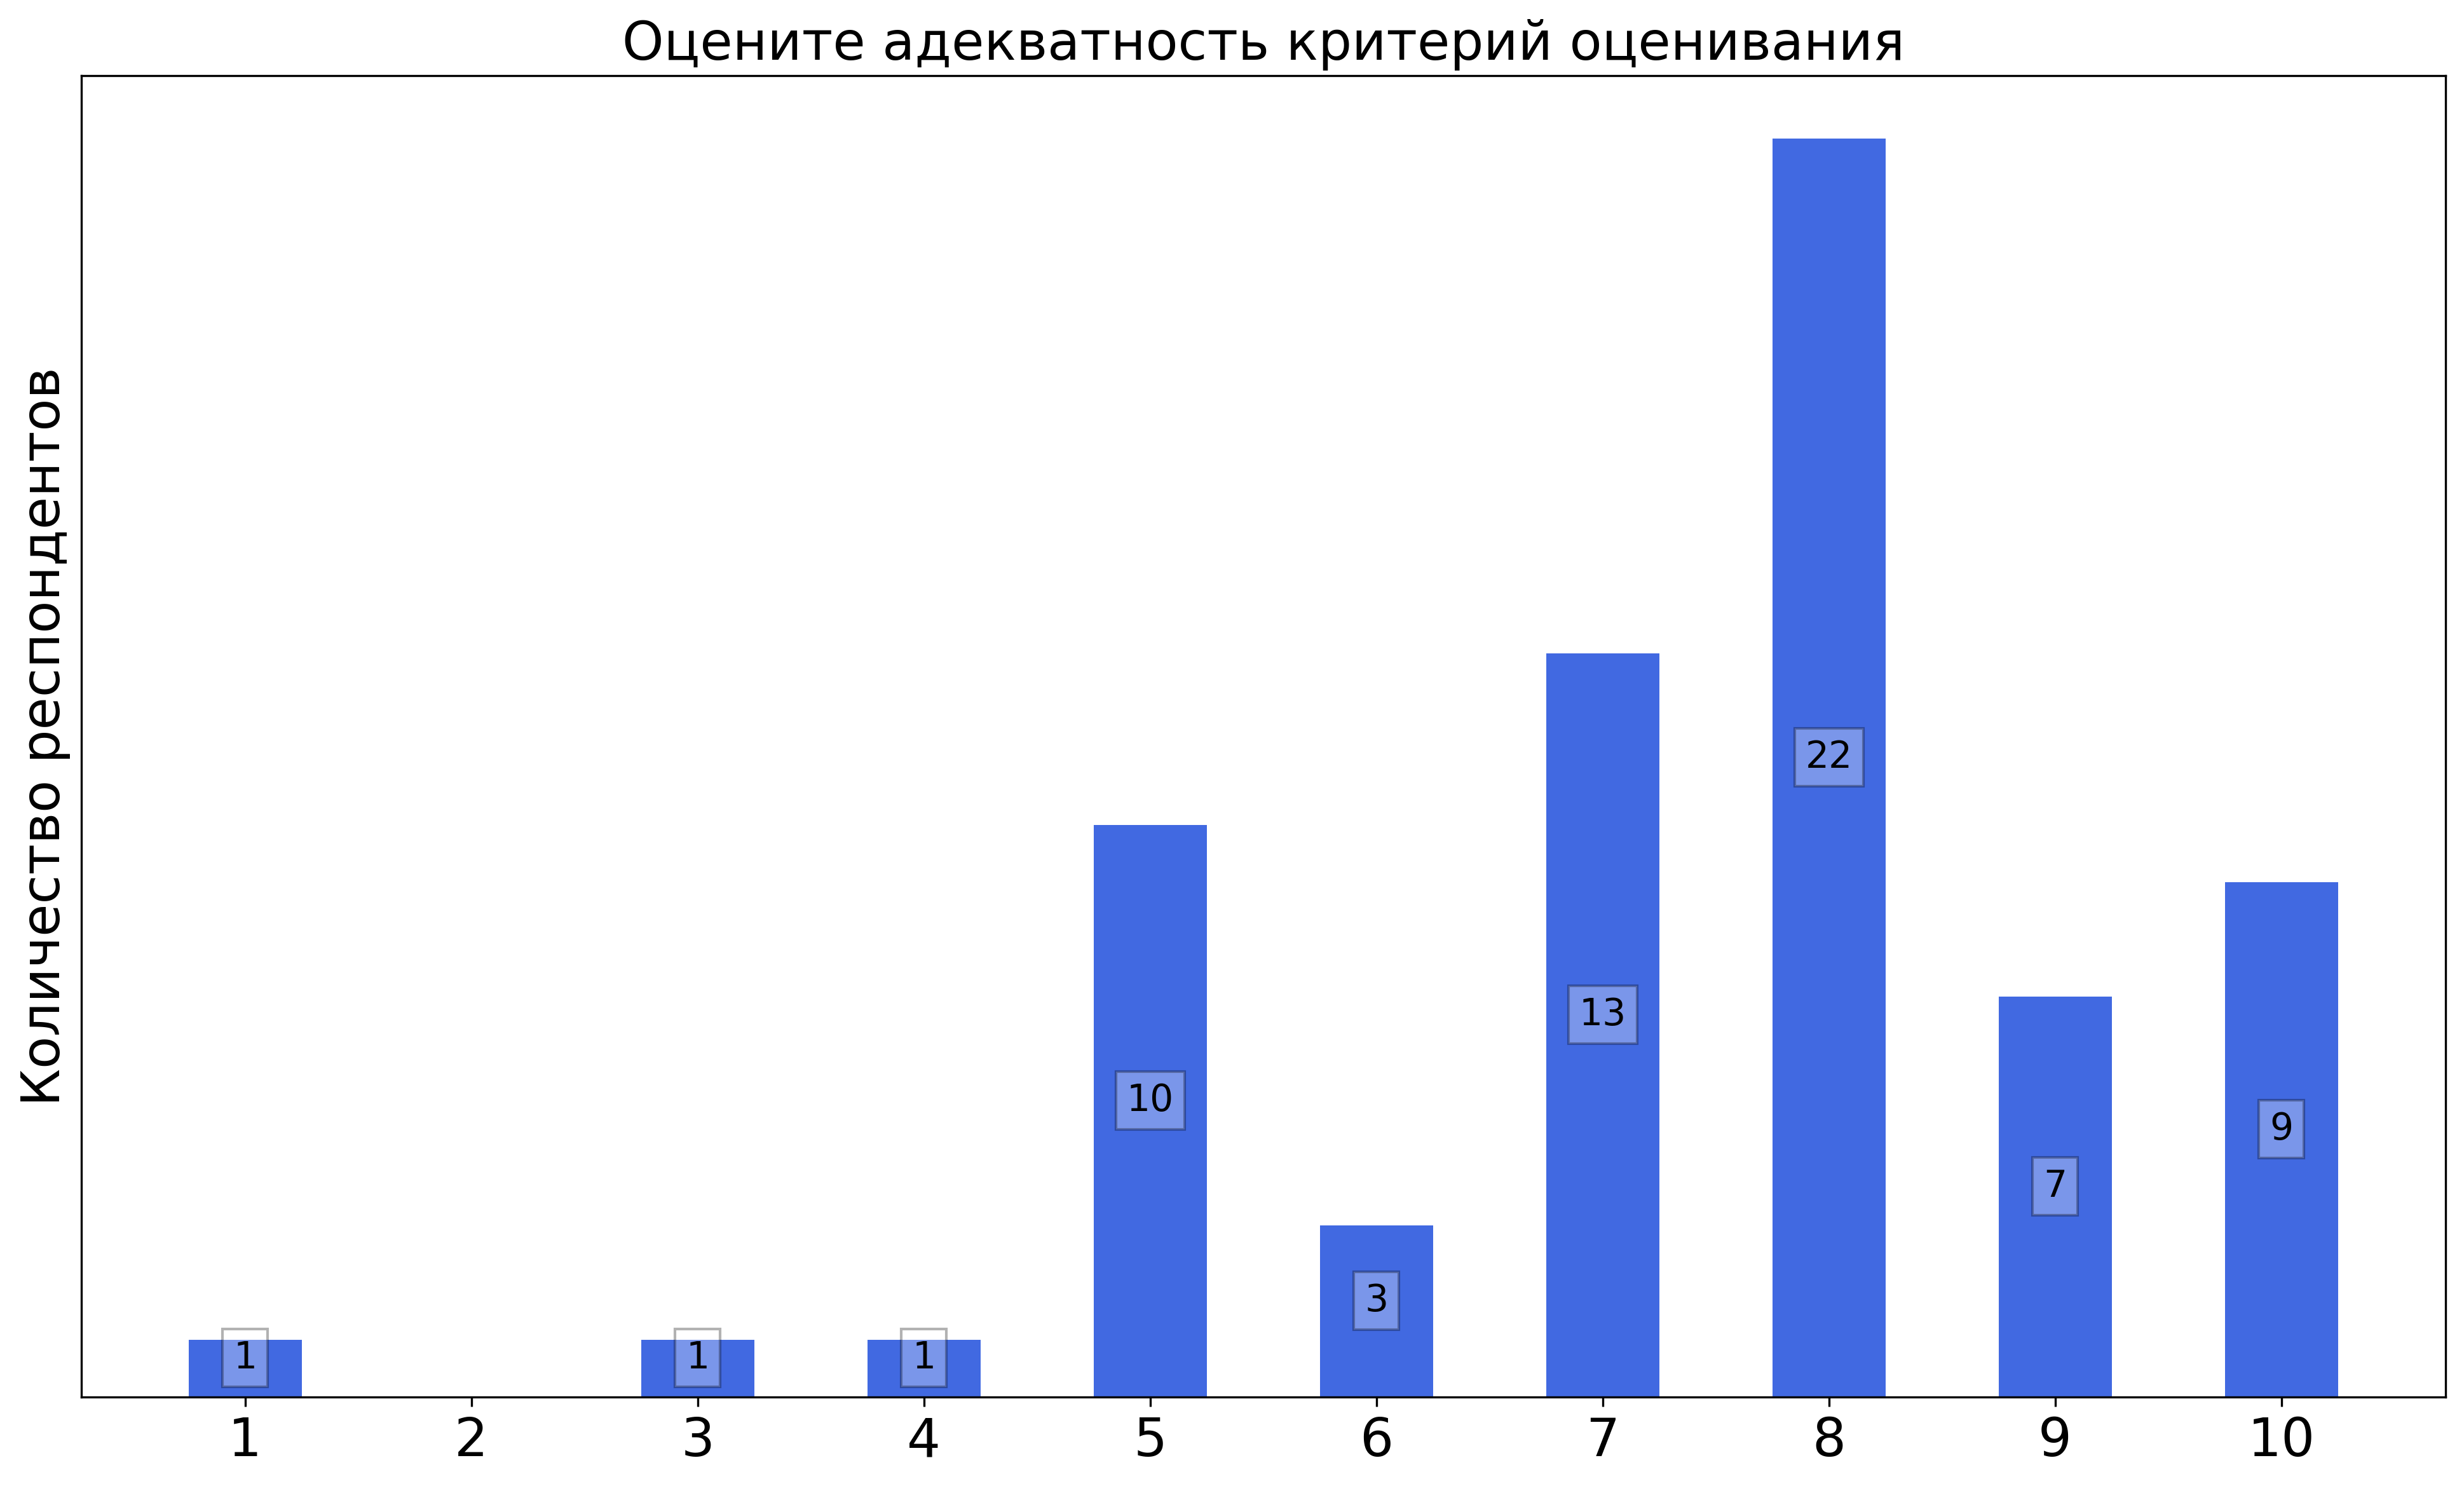
\includegraphics[width=\textwidth]{images/3 course/Теория поля/general-1.png}
			\end{subfigure}	
		\end{figure}

	\subsubsection{Материалы, использумые респондентами при изучении курса}

		\begin{figure}[H]
			\centering
			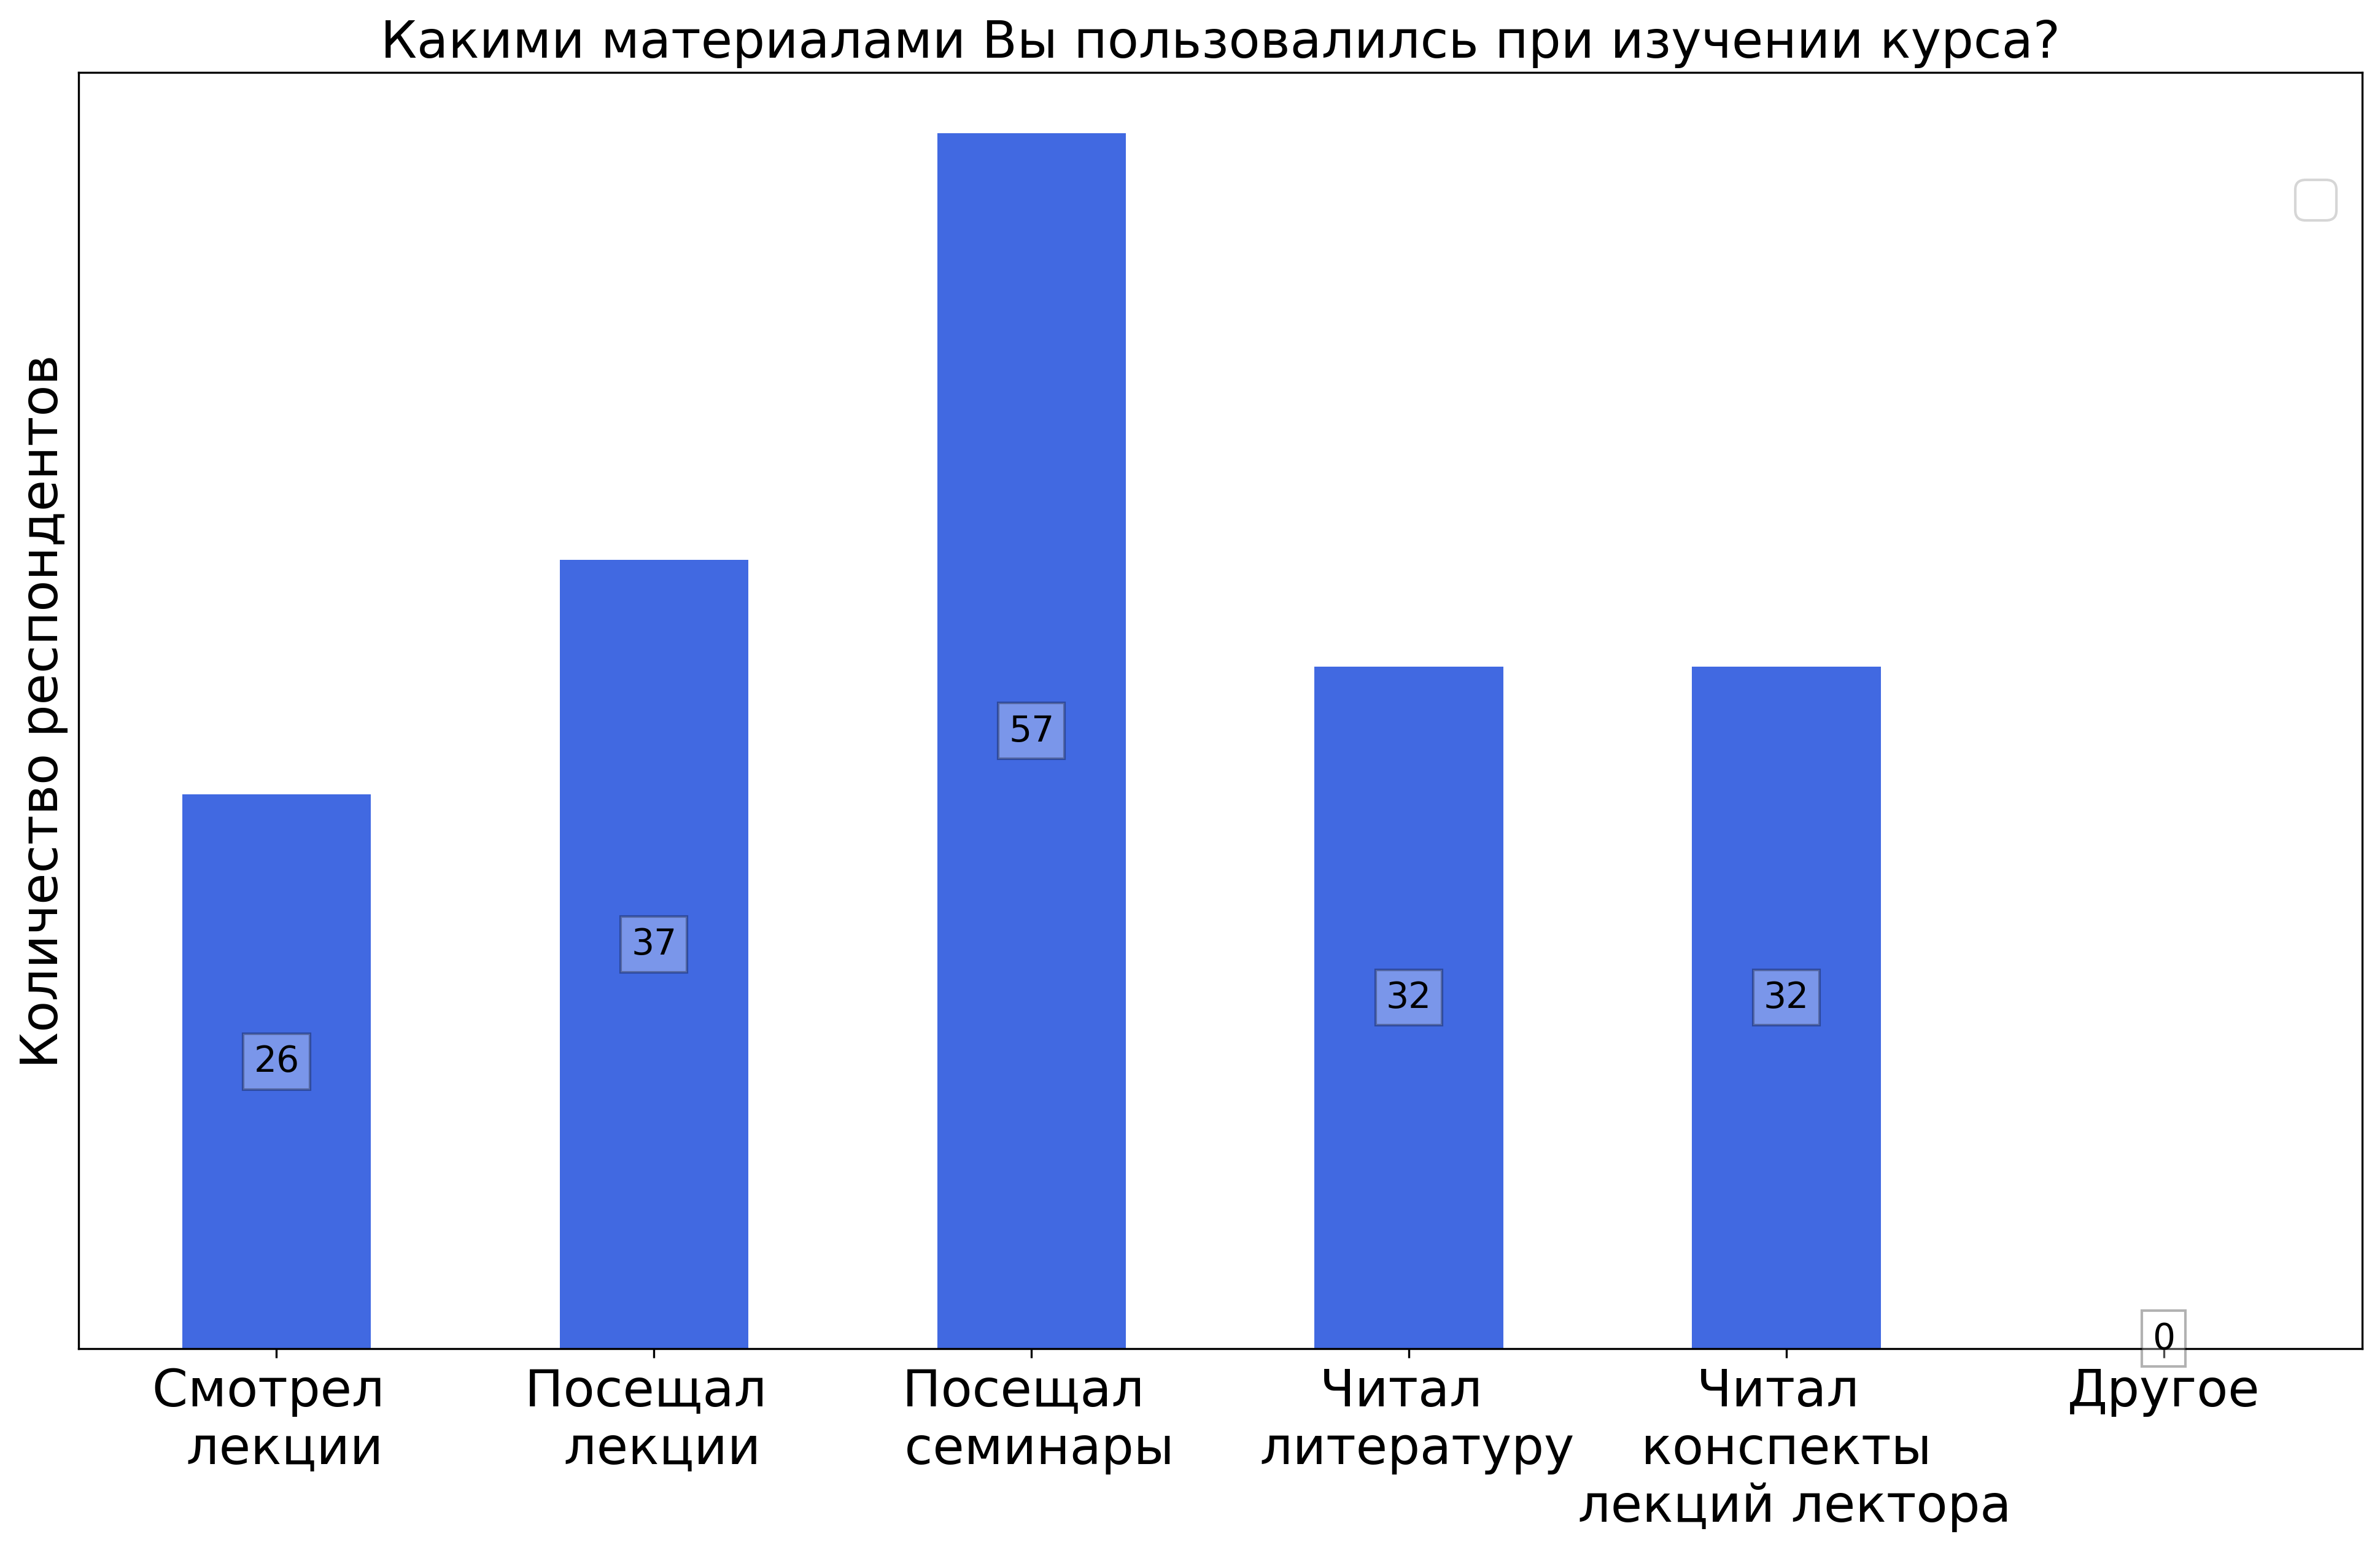
\includegraphics[width = 0.45\textwidth]{images/3 course/Теория поля/materials.png}
		\end{figure}

	\subsubsection{Отзыв студентов о лекциях. Лектор: Гец А.В.}

		\begin{figure}[H]
			\centering
            \begin{subfigure}[b]{0.45\textwidth}
				\centering
				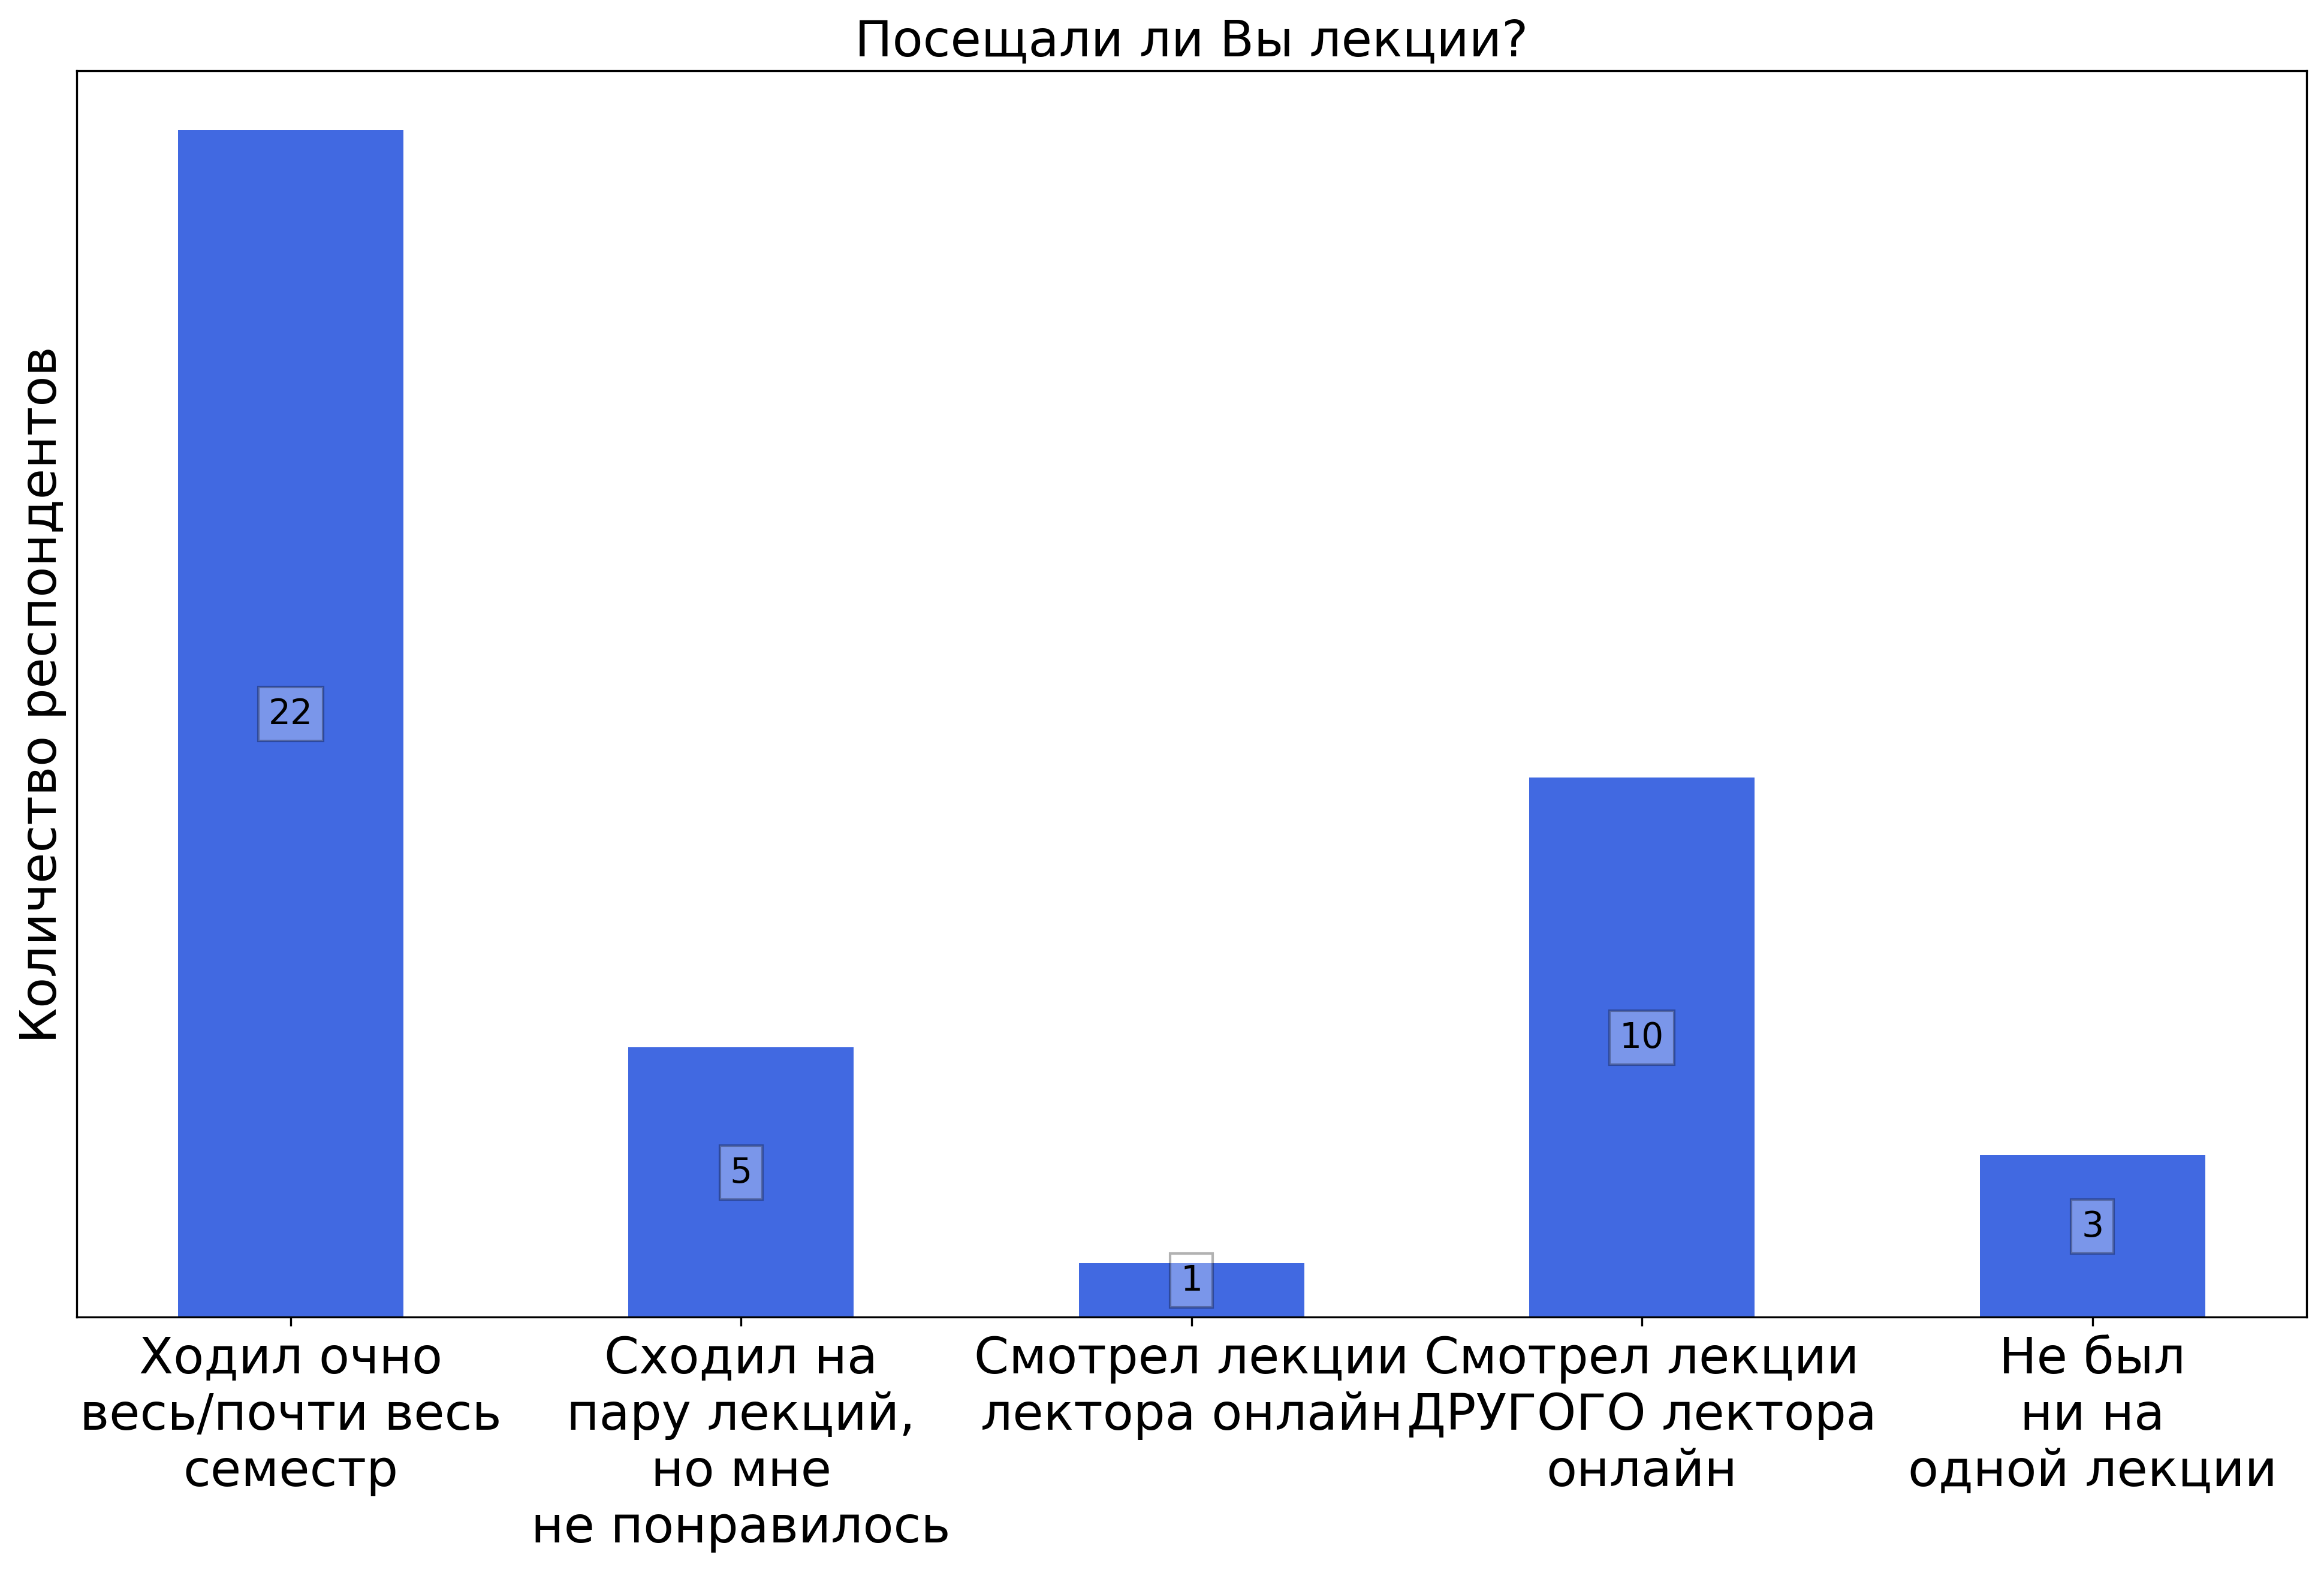
\includegraphics[width=\textwidth]{images/3 course/Теория поля/lecturer-questions-Гец А.В.-0.png}
			\end{subfigure}
			\begin{subfigure}[b]{0.45\textwidth}
				\centering
				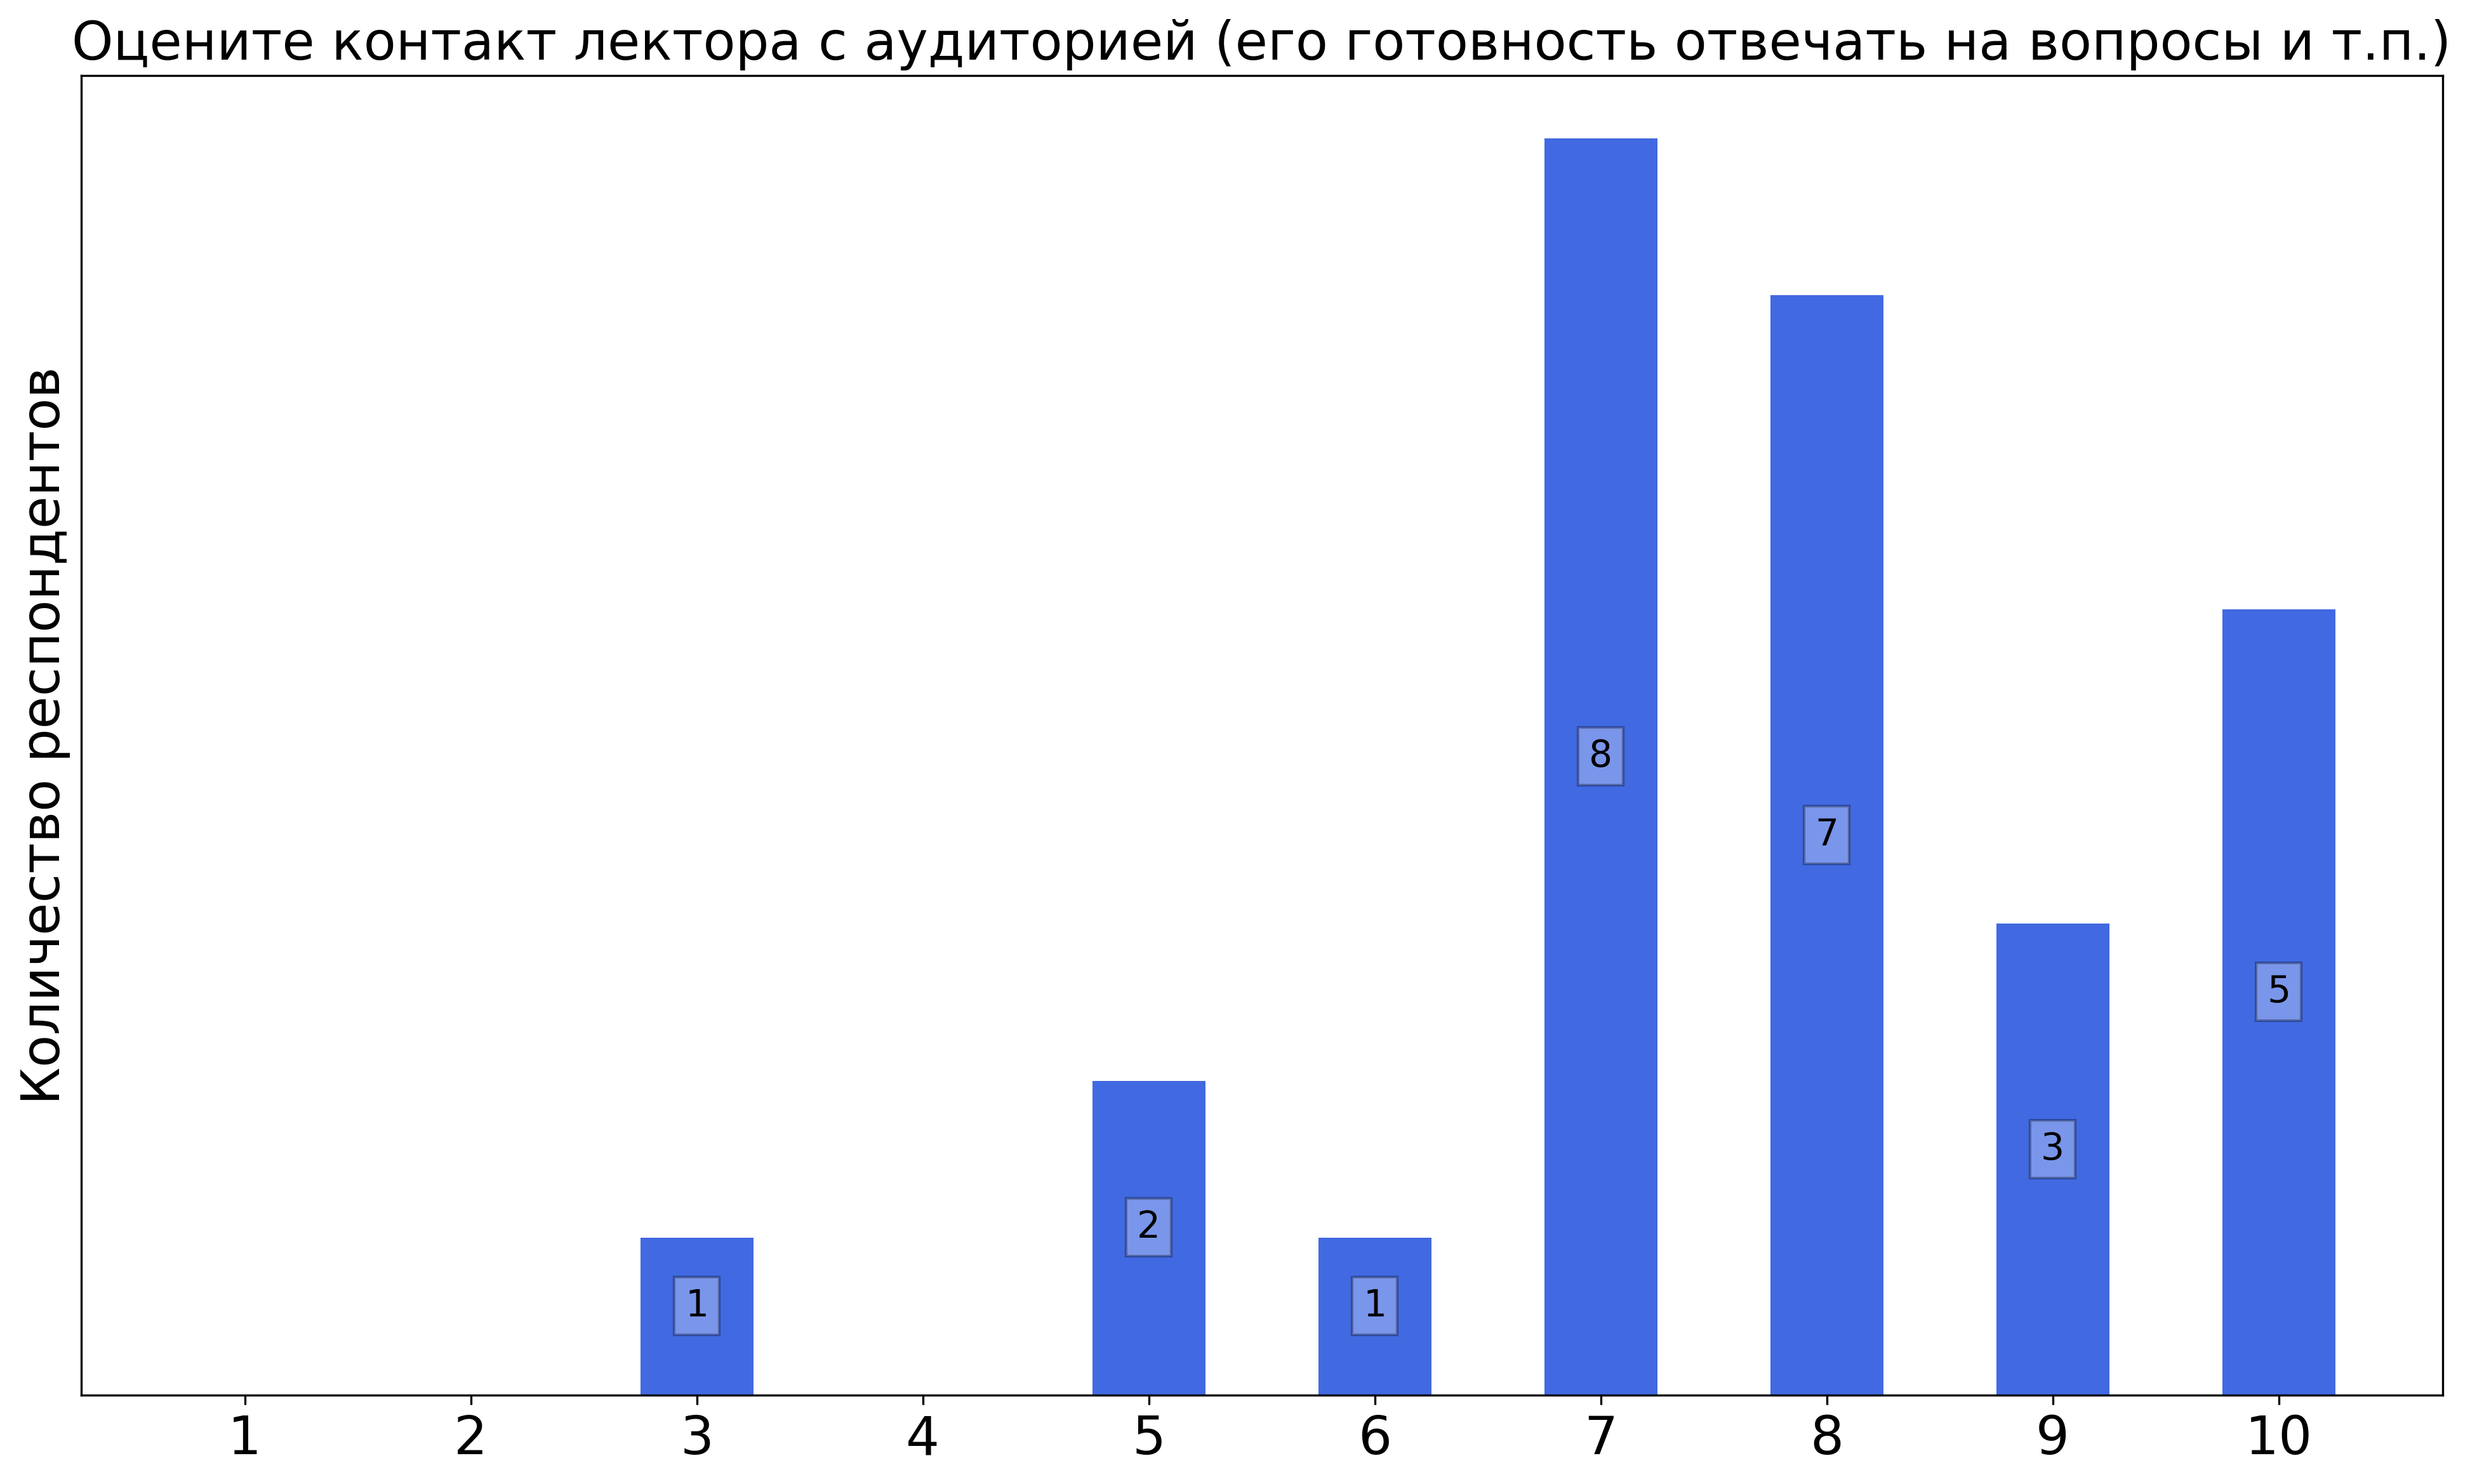
\includegraphics[width=\textwidth]{images/3 course/Теория поля/lecturer-marks-Гец А.В.-0.png}
			\end{subfigure}
			\begin{subfigure}[b]{0.45\textwidth}
				\centering
				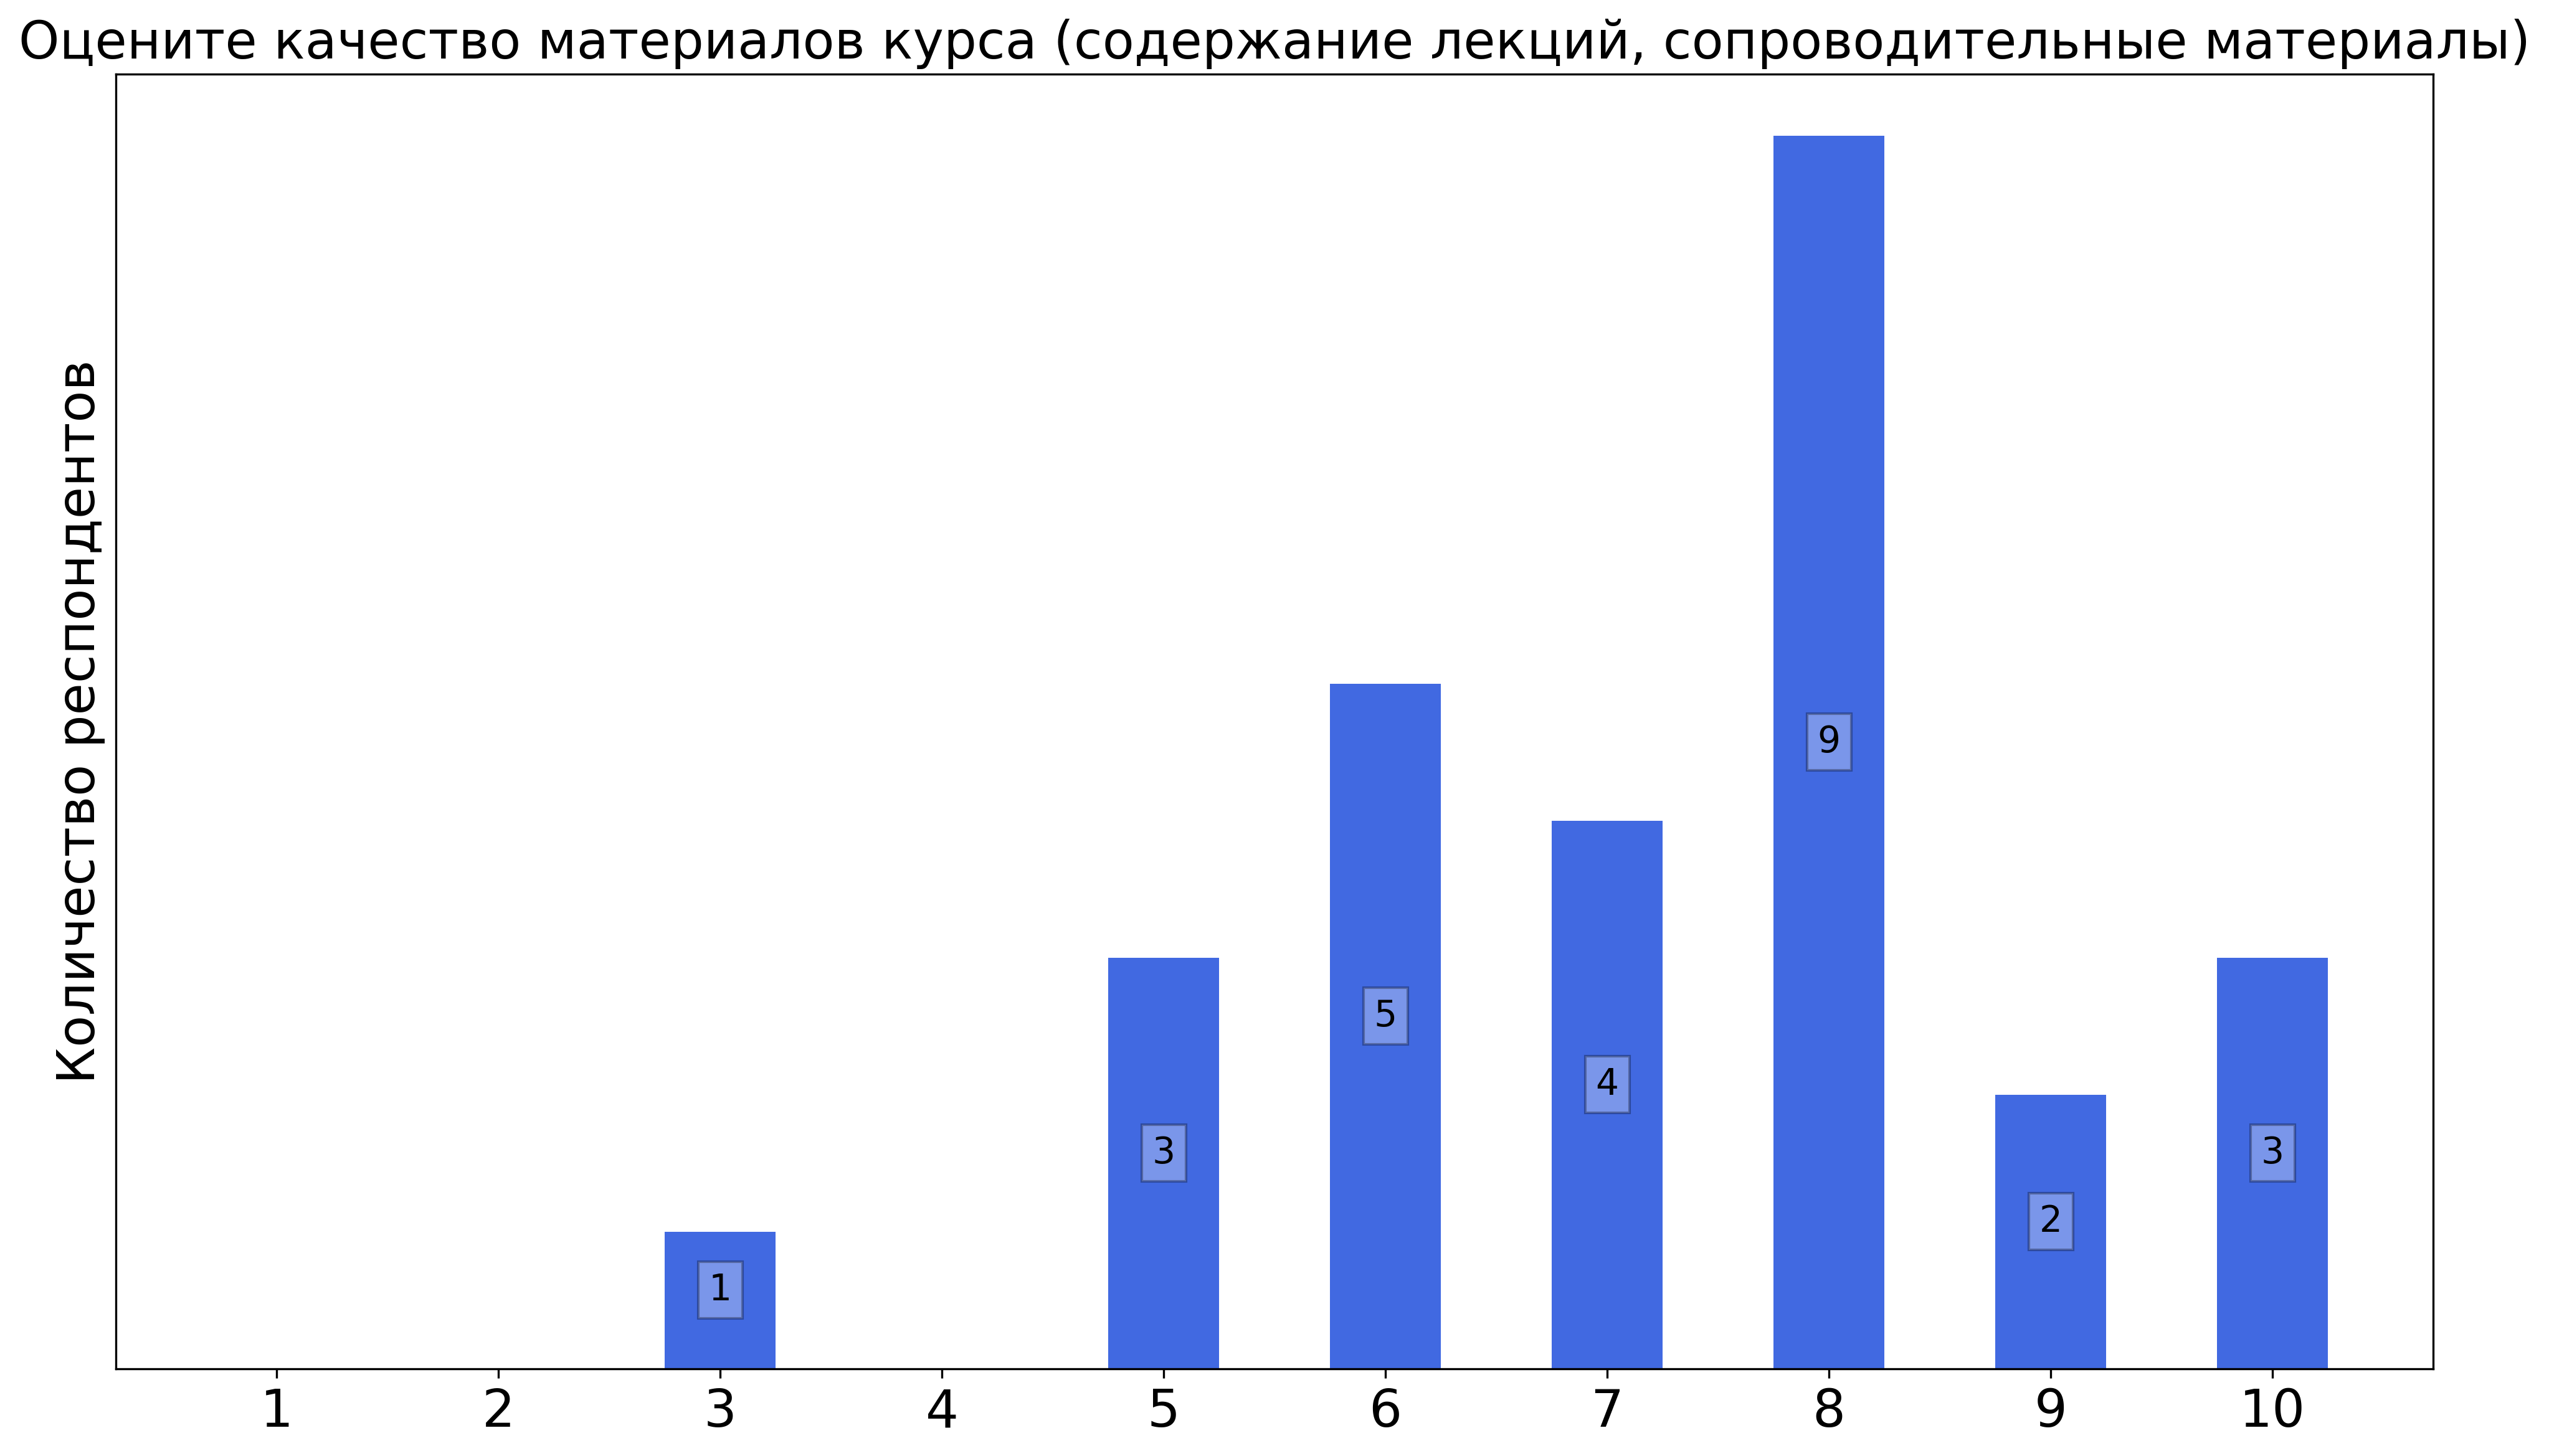
\includegraphics[width=\textwidth]{images/3 course/Теория поля/lecturer-marks-Гец А.В.-1.png}
			\end{subfigure}
			\begin{subfigure}[b]{0.45\textwidth}
				\centering
				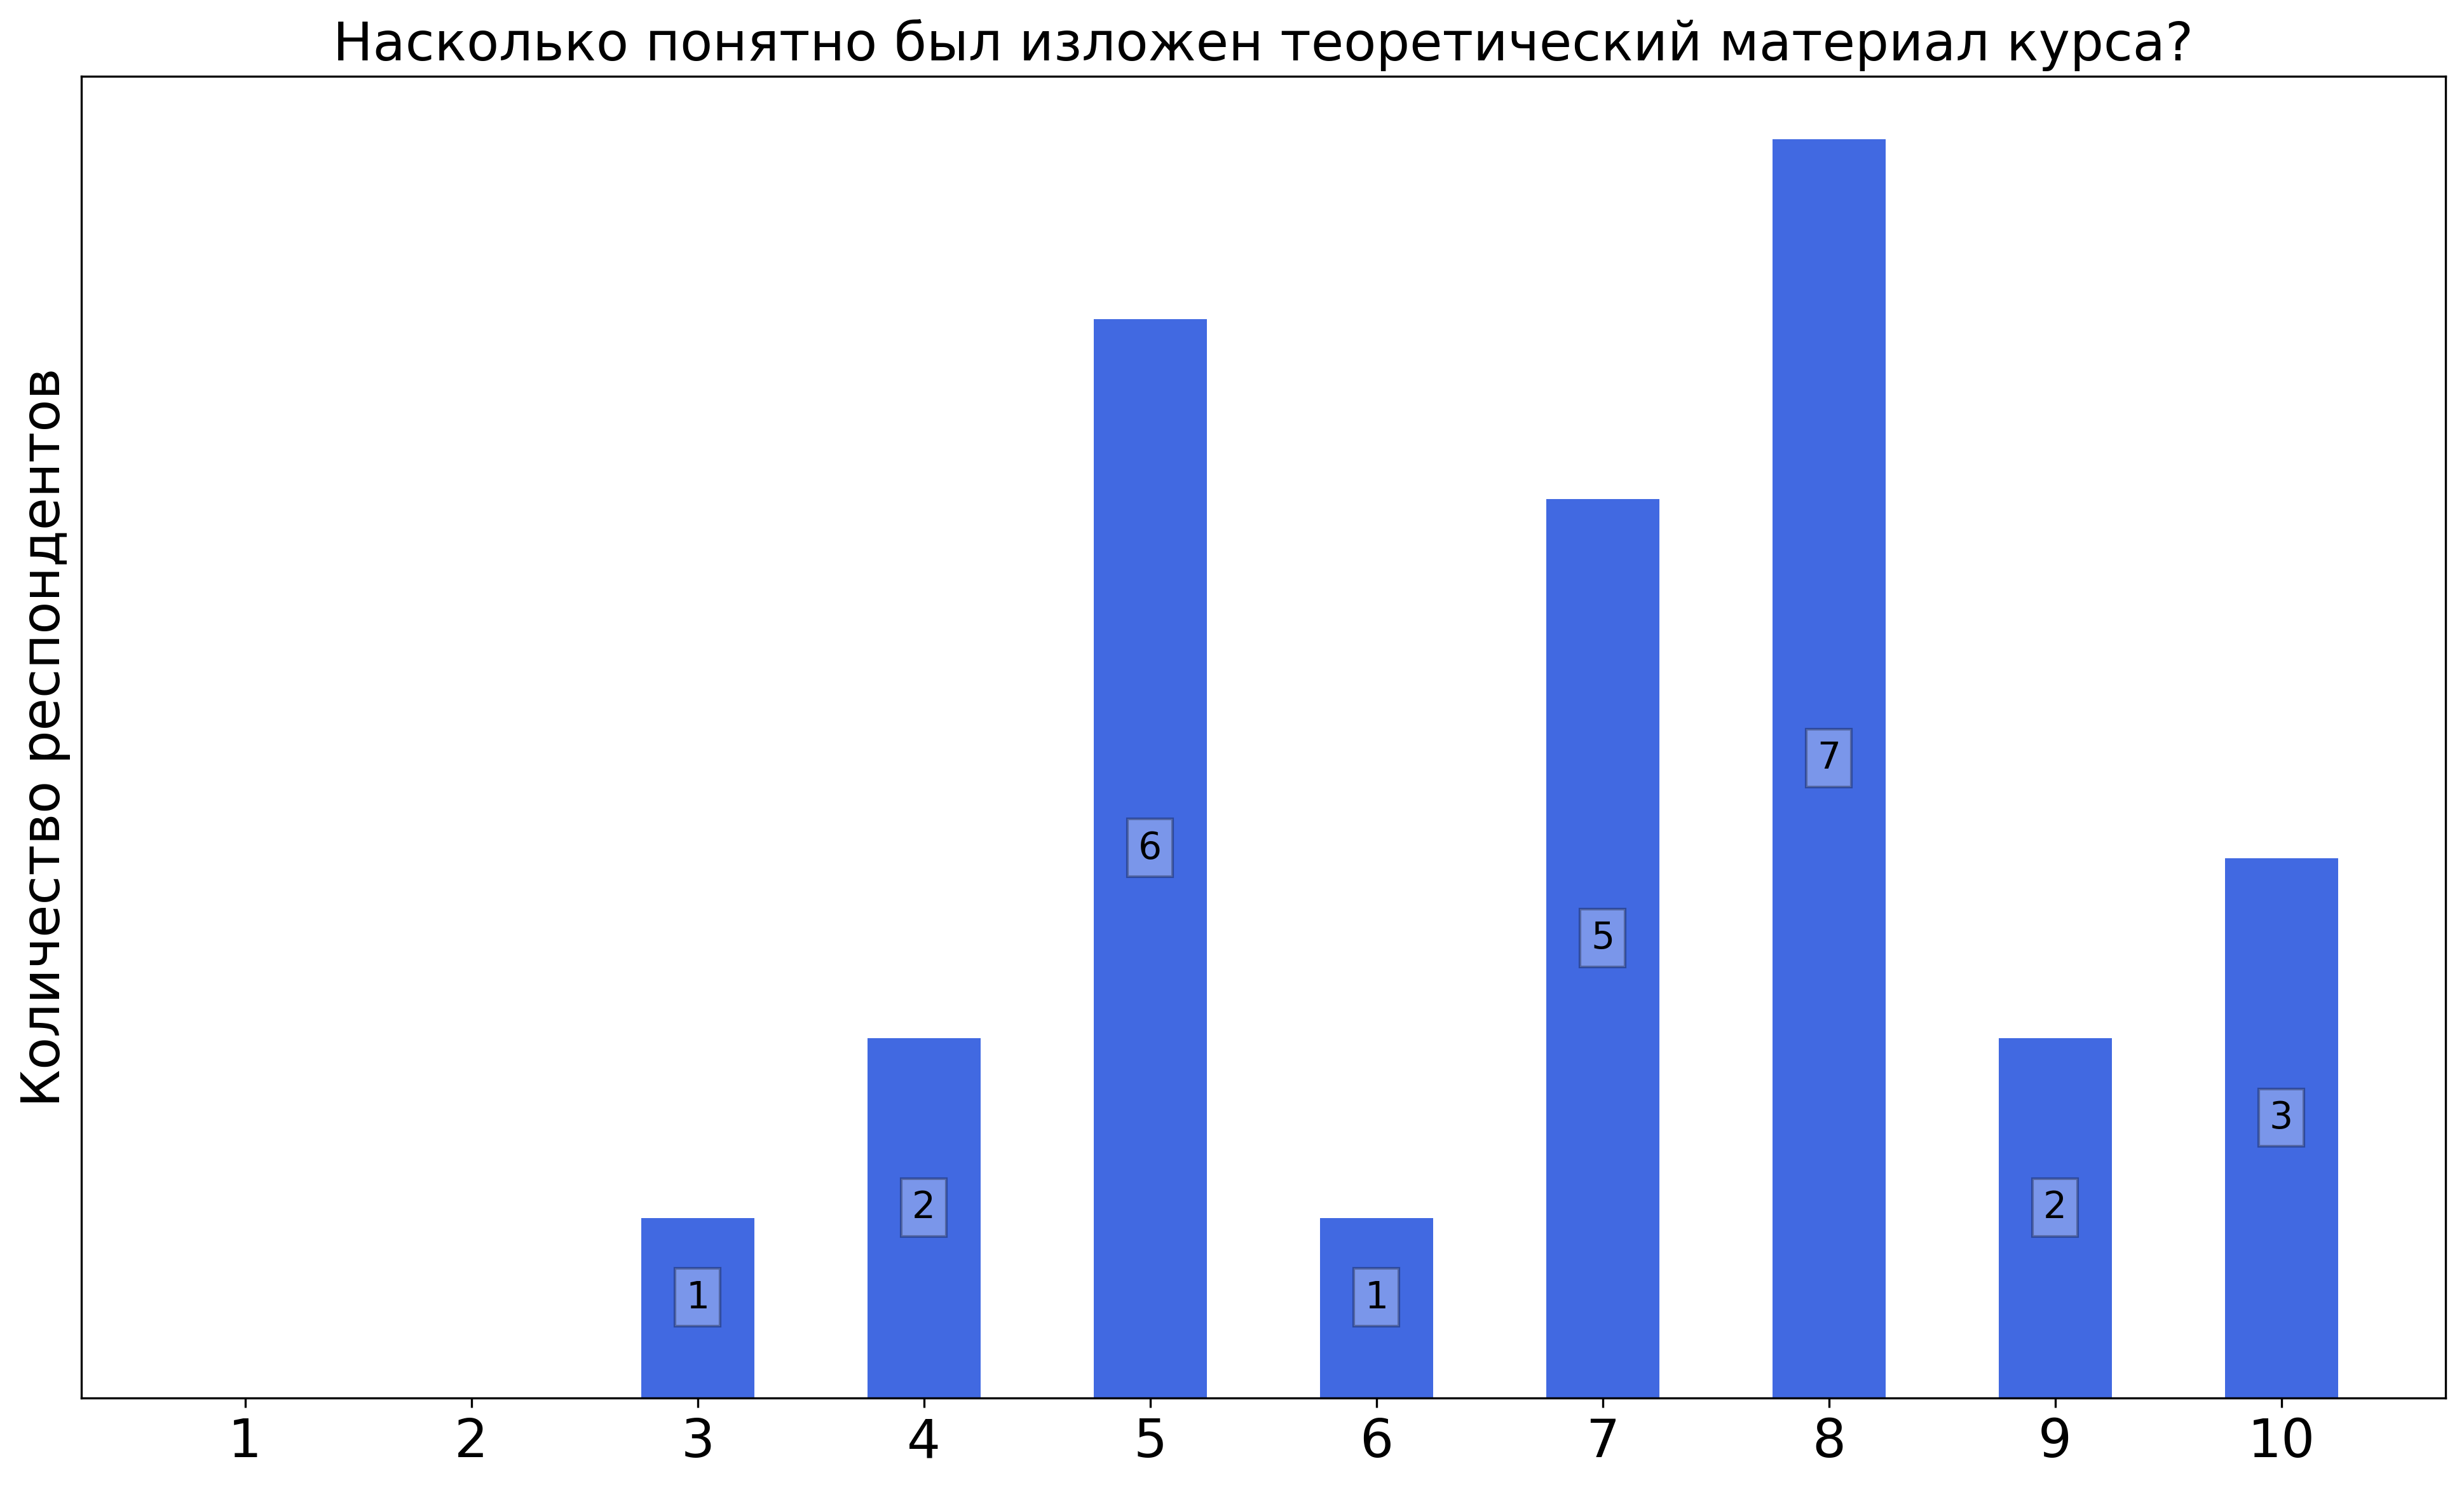
\includegraphics[width=\textwidth]{images/3 course/Теория поля/lecturer-marks-Гец А.В.-2.png}
			\end{subfigure}	
			\begin{subfigure}[b]{0.45\textwidth}
				\centering
				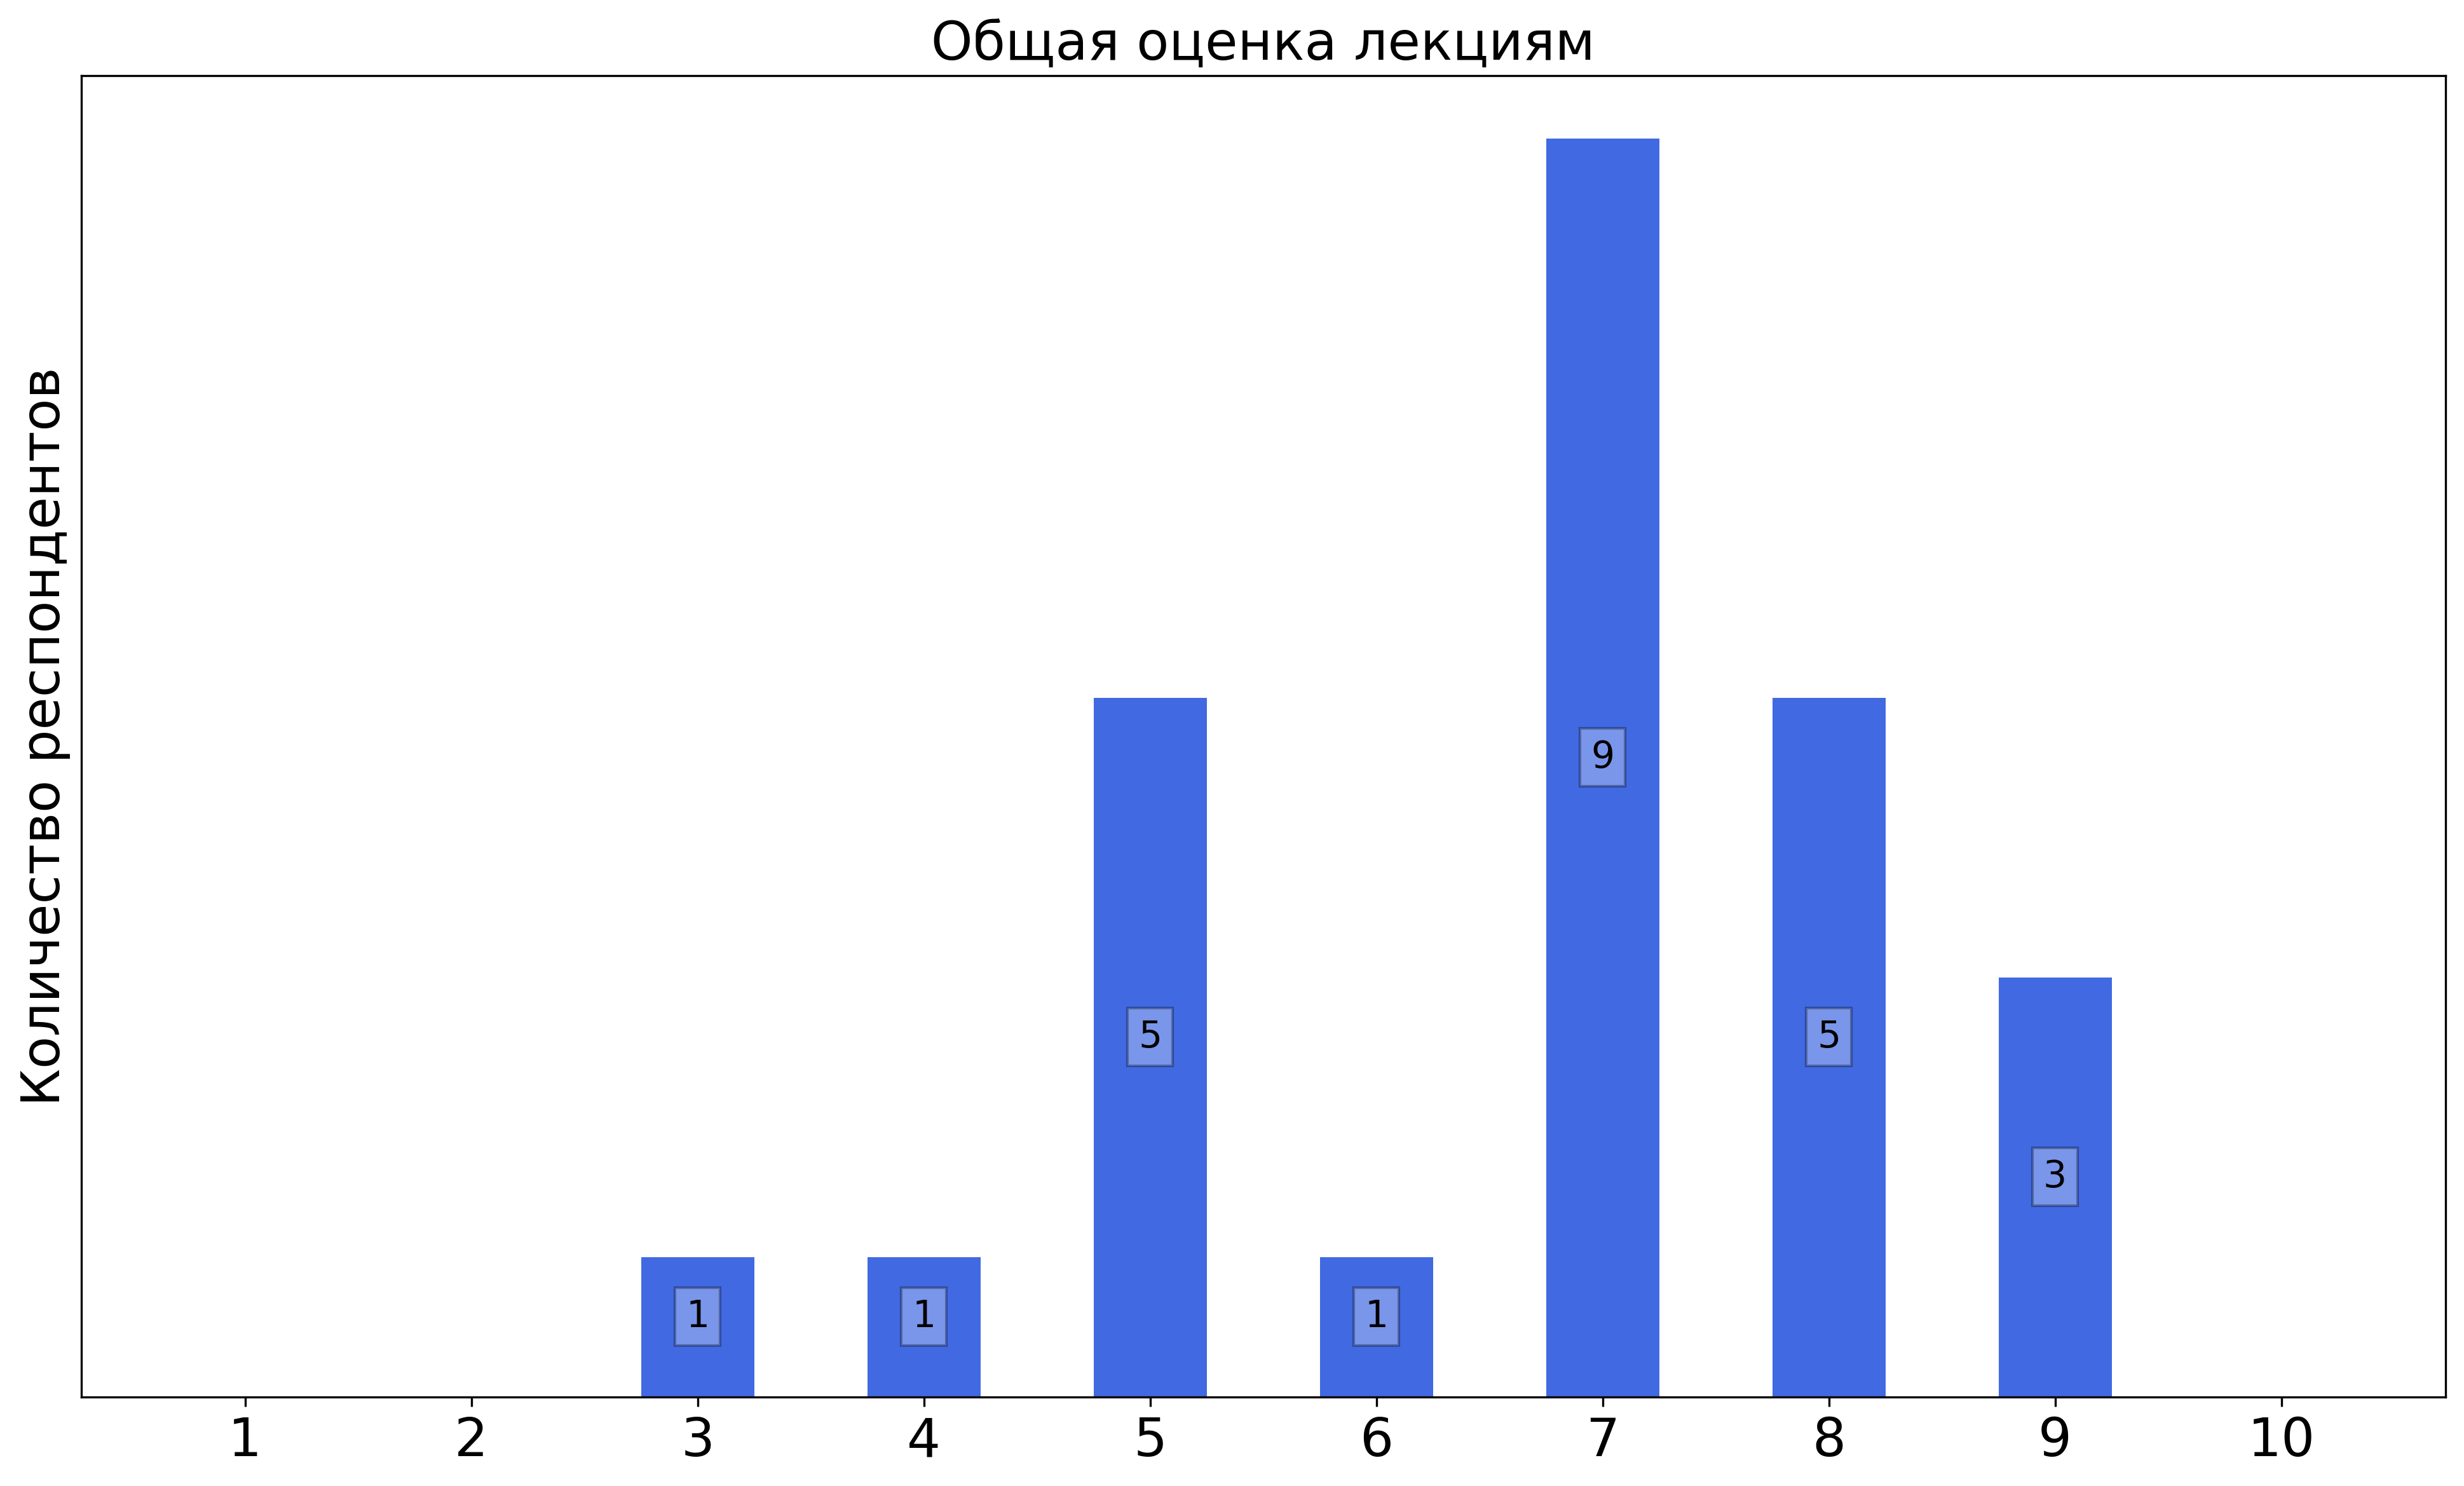
\includegraphics[width=\textwidth]{images/3 course/Теория поля/lecturer-marks-Гец А.В.-3.png}
			\end{subfigure}
			\caption{Оценки респондентов о качестве преподавания лекций по курсу <<Теория поля>>}
		\end{figure}

		\textbf{Комментарии студентов о лекциях\protect\footnote{сохранены оригинальные орфография и пунктуация}}
            \begin{commentbox} 
                Лекции читаются "уныло", объясняется материал тоже не очень понятно. Поэтому, если учиться по лекциям лектора, то нужно заглядывать постоянно в Ландавшиц, чтобы понять материал 
            \end{commentbox} 
        
            \begin{commentbox} 
                В начале лектор шел очень медленно, так как ждал понимания рассказанного, но его не могло быть, так как введения в тензоры в курсе не было, и все закономерно казалось магией. Так же вначале много ошибался, так как пытался рассказывать без листа. Потом стало гораздо лучше, темп увеличился, ошибок не было. Но все равно очень много мы не покрыли, не успели, последние лекции прошли в спешке.  
            \end{commentbox} 
        
            \begin{commentbox} 
                Лектор хороший, отставали, конечно, от программы, но в общих чертах лекционный курс хороший  
            \end{commentbox} 
        
            \begin{commentbox} 
                Начал медленно курс, из-за чего большая часть реально важного была изложена под самый конец, задерживал лекции 
            \end{commentbox} 
        
            \begin{commentbox} 
                Лектор слишком медленно читает, при этом до мельчайших подробностей проговаривая очевидные вещи. В целом данный материал был хорошо понятен 
            \end{commentbox} 
        
            \begin{commentbox} 
                Неплохие лекции, вопросы лишь к дисциплине: были и опоздания, и долго непроверенные контрольные, и сорокаминутные поиски ошибки в выкладках. 
            \end{commentbox} 
        
            \begin{commentbox} 
                Лектор не успел прочитать материал в основное время лекций, поэтому были дополнительные(которые не были обговорены в расписании). Из приятного: материал четко структурирован и понятен. 
            \end{commentbox} 
        
            \begin{commentbox} 
                Гец в целом хороший лектор, но ничего не успевает, важные и сложные темы изложены комкано за 2 часа на последней лекции. Даёт сложные нерешаемые контрольные на короткое время 
            \end{commentbox} 
        
            \begin{commentbox} 
                Хороший лектор. Шарит, хорошо рассказывает. Иногда уходит в написание формул, теряя суть. Ландавшиц лучше написан :) 
                Тесты довольно сложные, а небольшие микротесты без предупреждения вынуждают посещать лекции (это плохо, если что) 
            \end{commentbox} 
        
            \begin{commentbox} 
                Мне не понравилась манера ведения лекций. В начале казалось, что лектор слишком медленно идет по программе, из-за чего не успевает. В конце он слишком ускорился и стал задерживать нас после пар. Объясняет вполне понятно, но есть определенные проблемы с распределением времени 
            \end{commentbox} 
        
            \begin{commentbox} 
                Часто ошибался и останавливался на несущественных местах из-за чего часто лекции задерживались сильно, а соответственно конец их был слишком скомканы. 
            \end{commentbox} 
        
            \begin{commentbox} 
                Лекции не очень хорошие. Подача материала немного сумбурная, всегда что-то не успевали. В целом ходить можно, но есть уже куда более хорошие записанные курсы других лекторов 
            \end{commentbox} 
        
            \begin{commentbox} 
                Мне не понравились лекции Артёма Викторовича, он читал материал тихо, непонятно и медленно, из-за чего польза очных лекций в течение семестра вызвала большие вопросы. Вместо этого я смотрел лекции Александра Викторовича Дорофеенко, которые оставили лишь положительное впечатление. 
            \end{commentbox} 
        
            \begin{commentbox} 
                Сами лекции не очень полезны, лучше читать ландавшица 
            \end{commentbox} 
        
            \begin{commentbox} 
                Лектор ужасен, говорит читать книжку, а лекции это не для того, чтобы учить нормально материал. Вопрос, зачем тогда нужен лектор непонятно, если он даже сам отвратительно объясняет и не помогает читать книжку. 
            \end{commentbox} 
        
            \begin{commentbox} 
                Не очень структурированные лекции.  
            \end{commentbox} 
        
            \begin{commentbox} 
                Лектор неплохой, но бывает что тупит у доски по-долгу, из-за этого трудно воспринимать материал. 
            \end{commentbox} 
        
            \begin{commentbox} 
                Хорошо знает материал, но медленно рассказывает в первой половине лекции, и к концу сильно  разгонятся, чтобы успеть. Контрольные на лекциях справедливые, можно спросить об ошибках. Рассказывает тихо, почти про себя , приходится прислушиваться. Очень мелко пишет.
            \end{commentbox}


    \subsubsection{Отзыв студентов о лекциях. Лектор: Фомичев С.В.}
		\begin{figure}[H]
			\centering
            \begin{subfigure}[b]{0.45\textwidth}
				\centering
				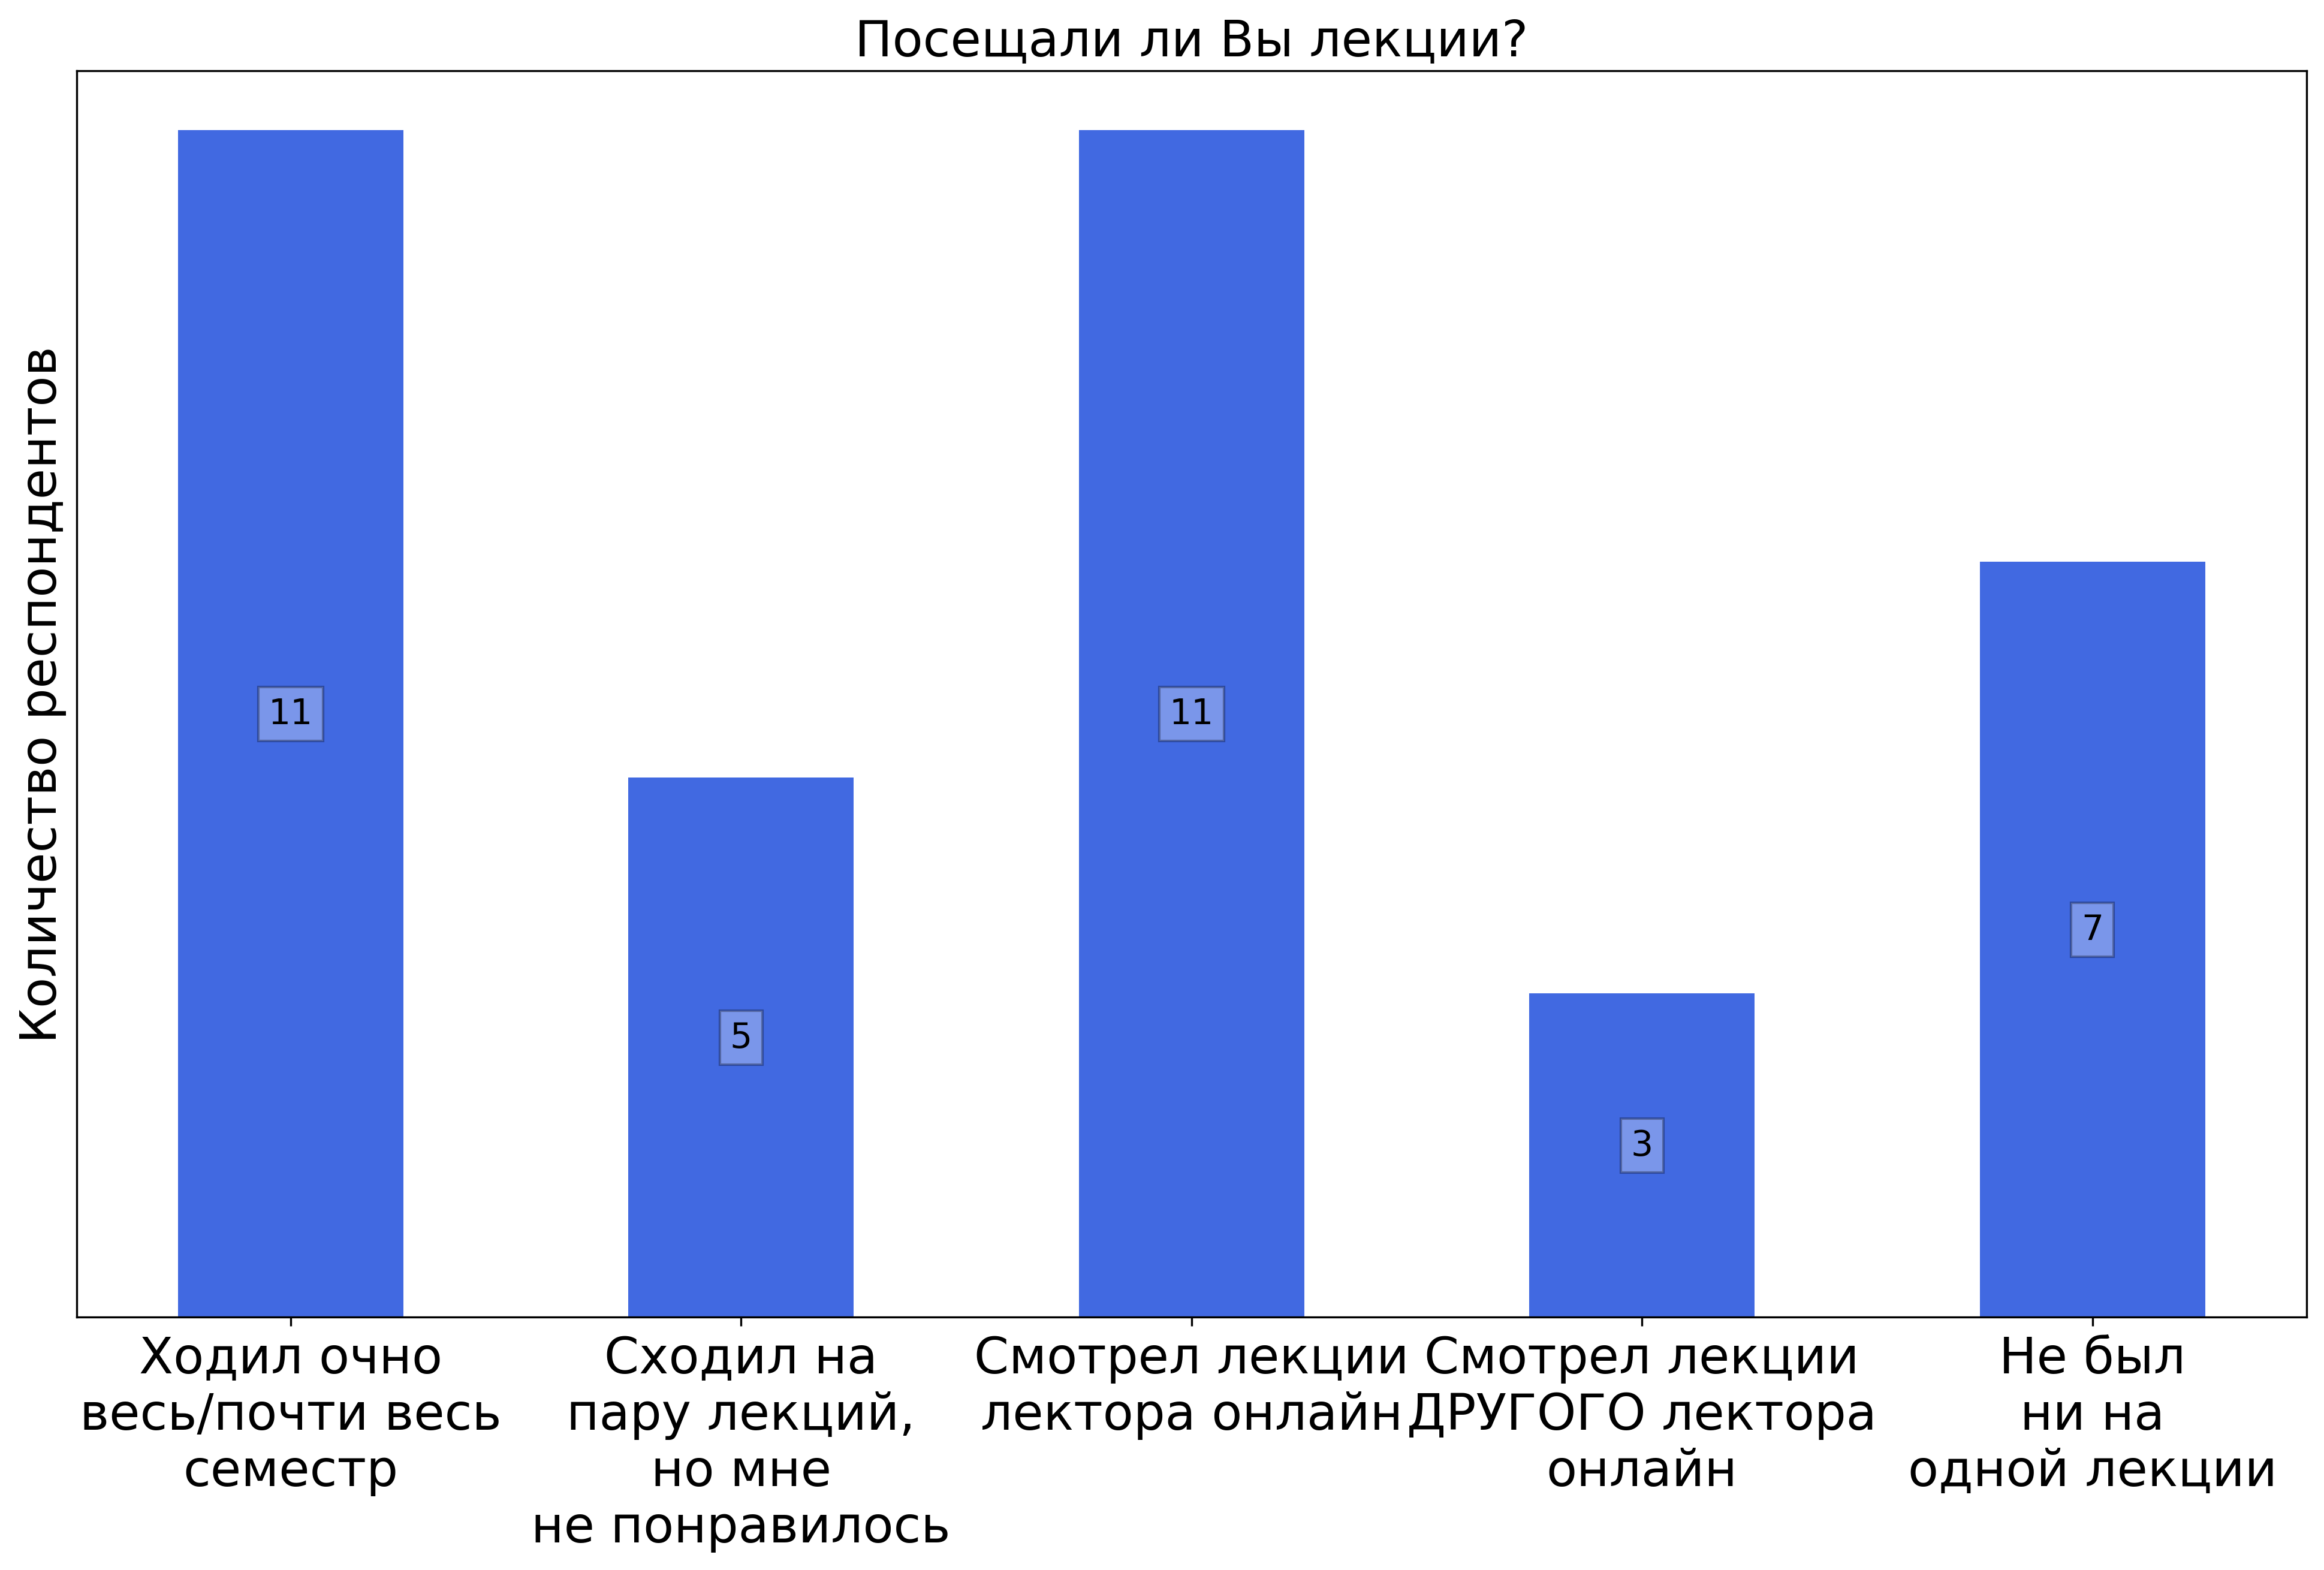
\includegraphics[width=\textwidth]{images/3 course/Теория поля/lecturer-questions-Фомичев С.В.-0.png}
			\end{subfigure}
			\begin{subfigure}[b]{0.45\textwidth}
				\centering
				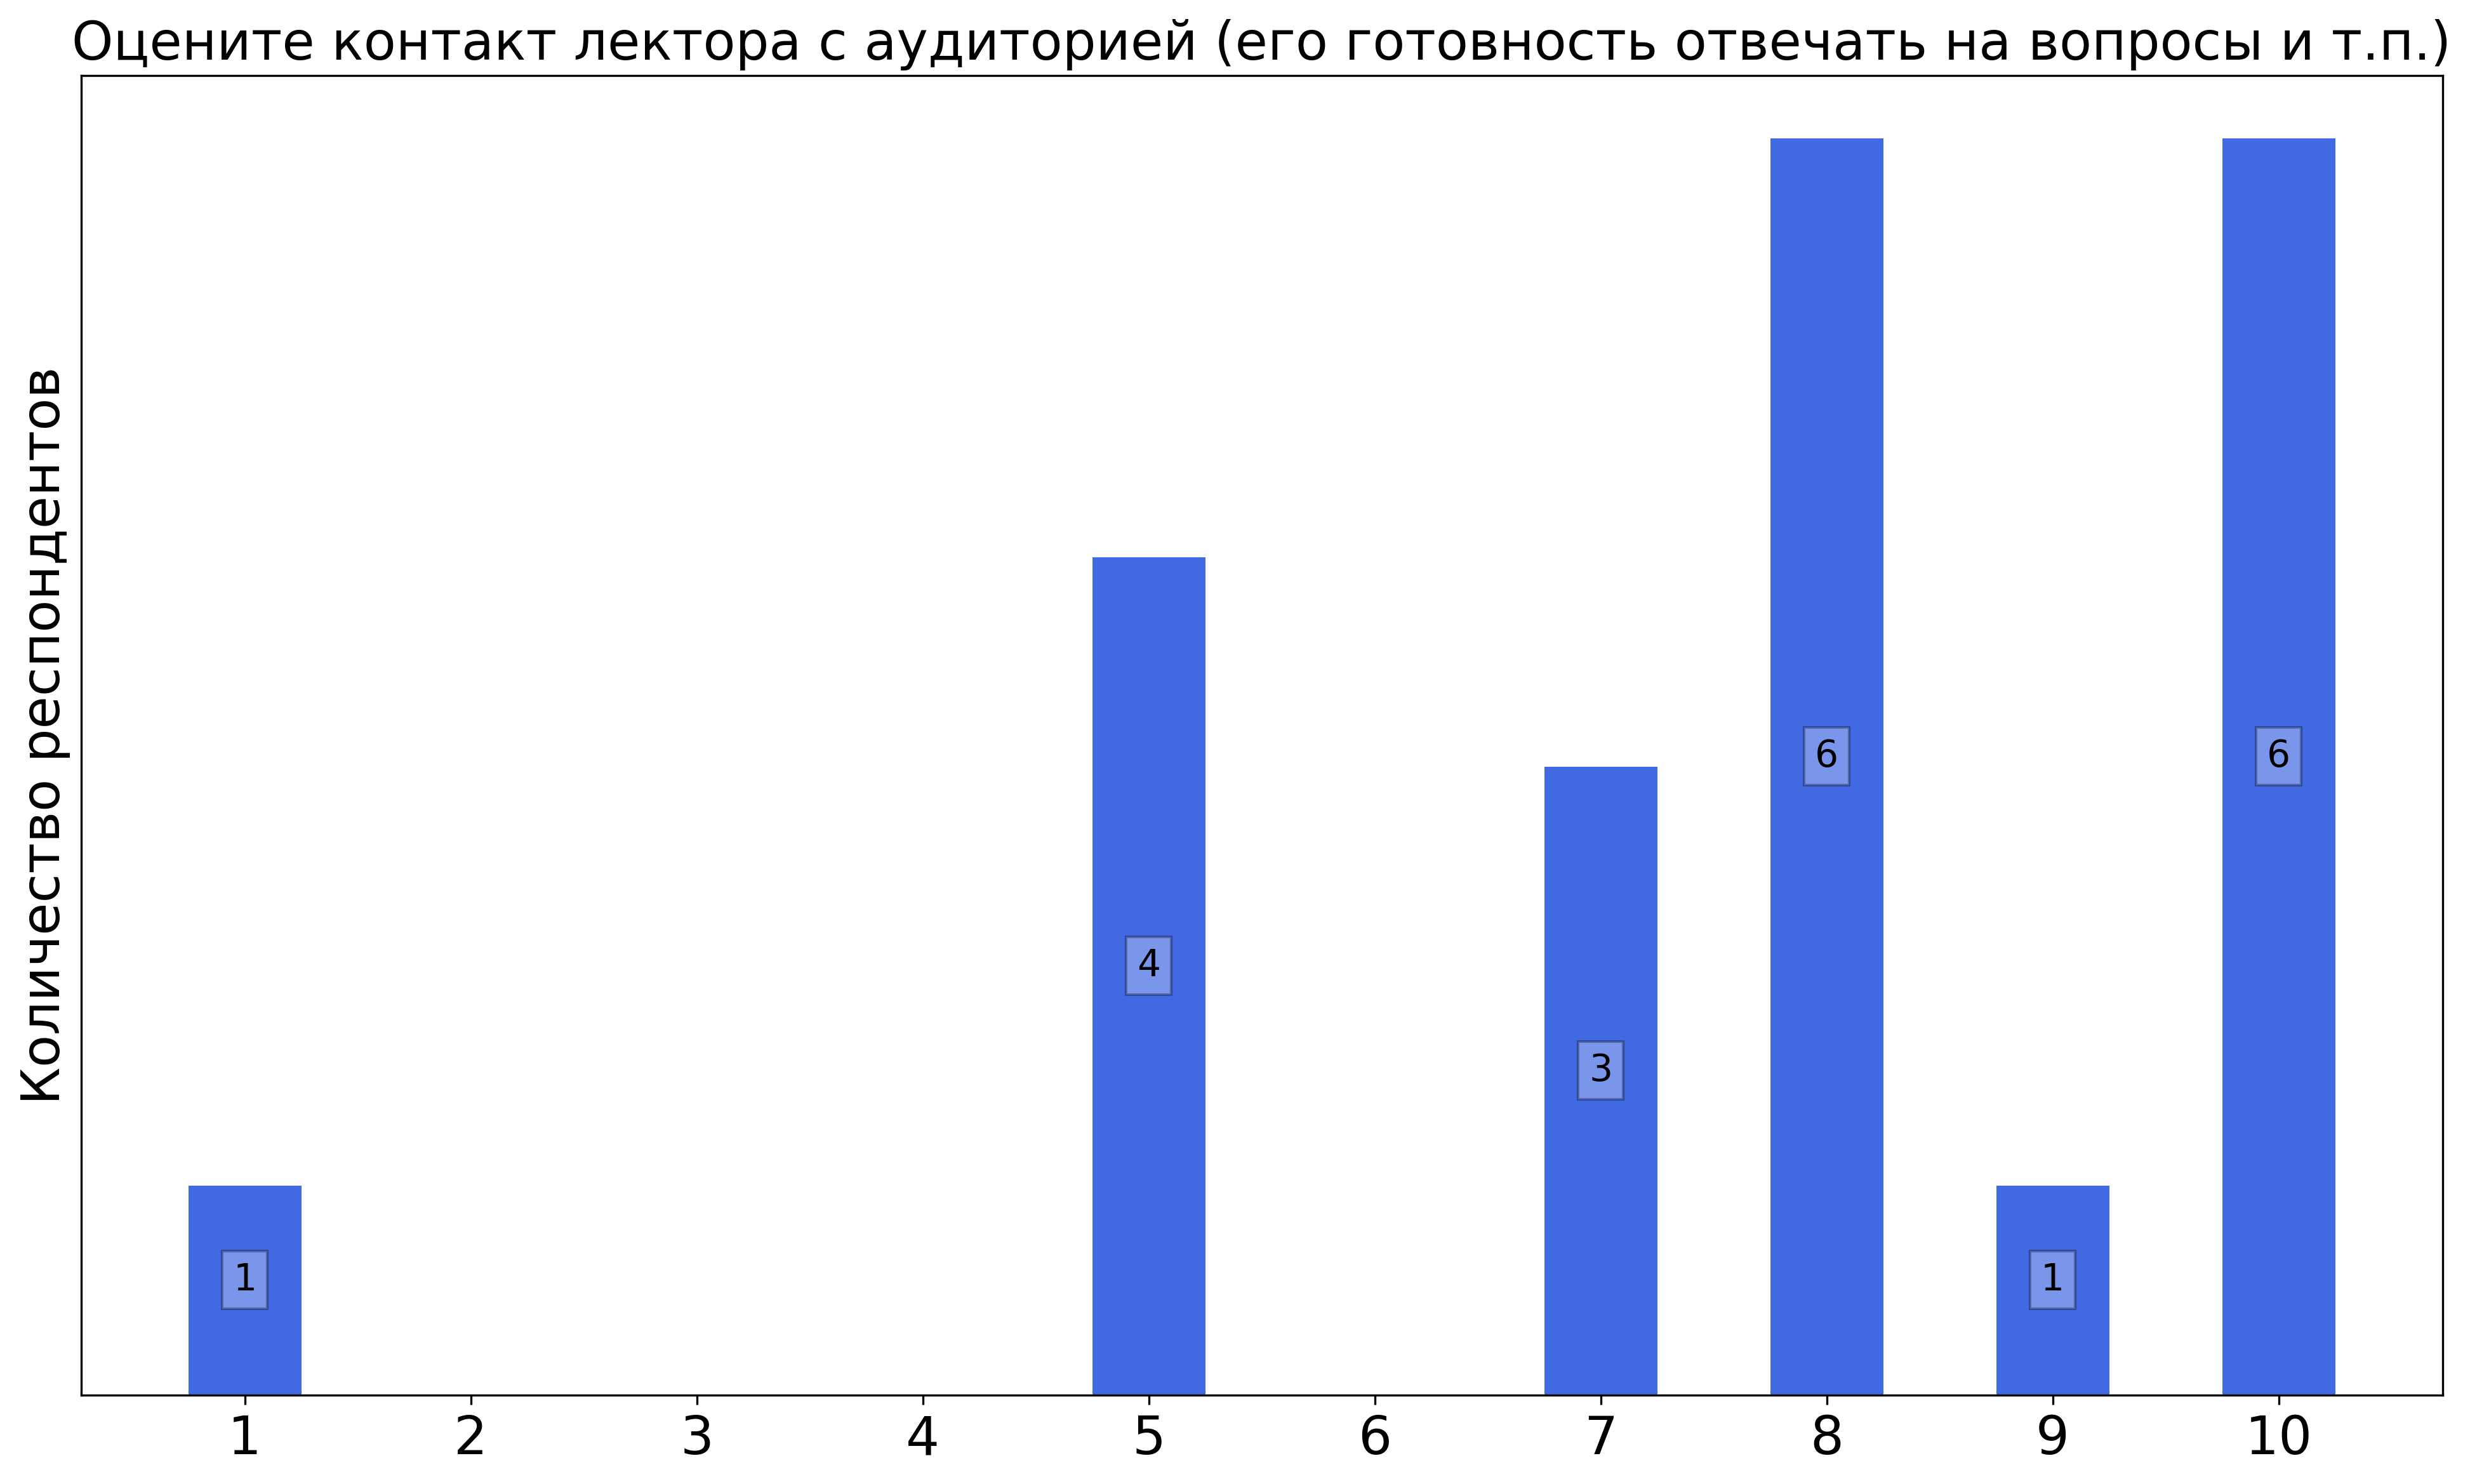
\includegraphics[width=\textwidth]{images/3 course/Теория поля/lecturer-marks-Фомичев С.В.-0.png}
			\end{subfigure}
			\begin{subfigure}[b]{0.45\textwidth}
				\centering
				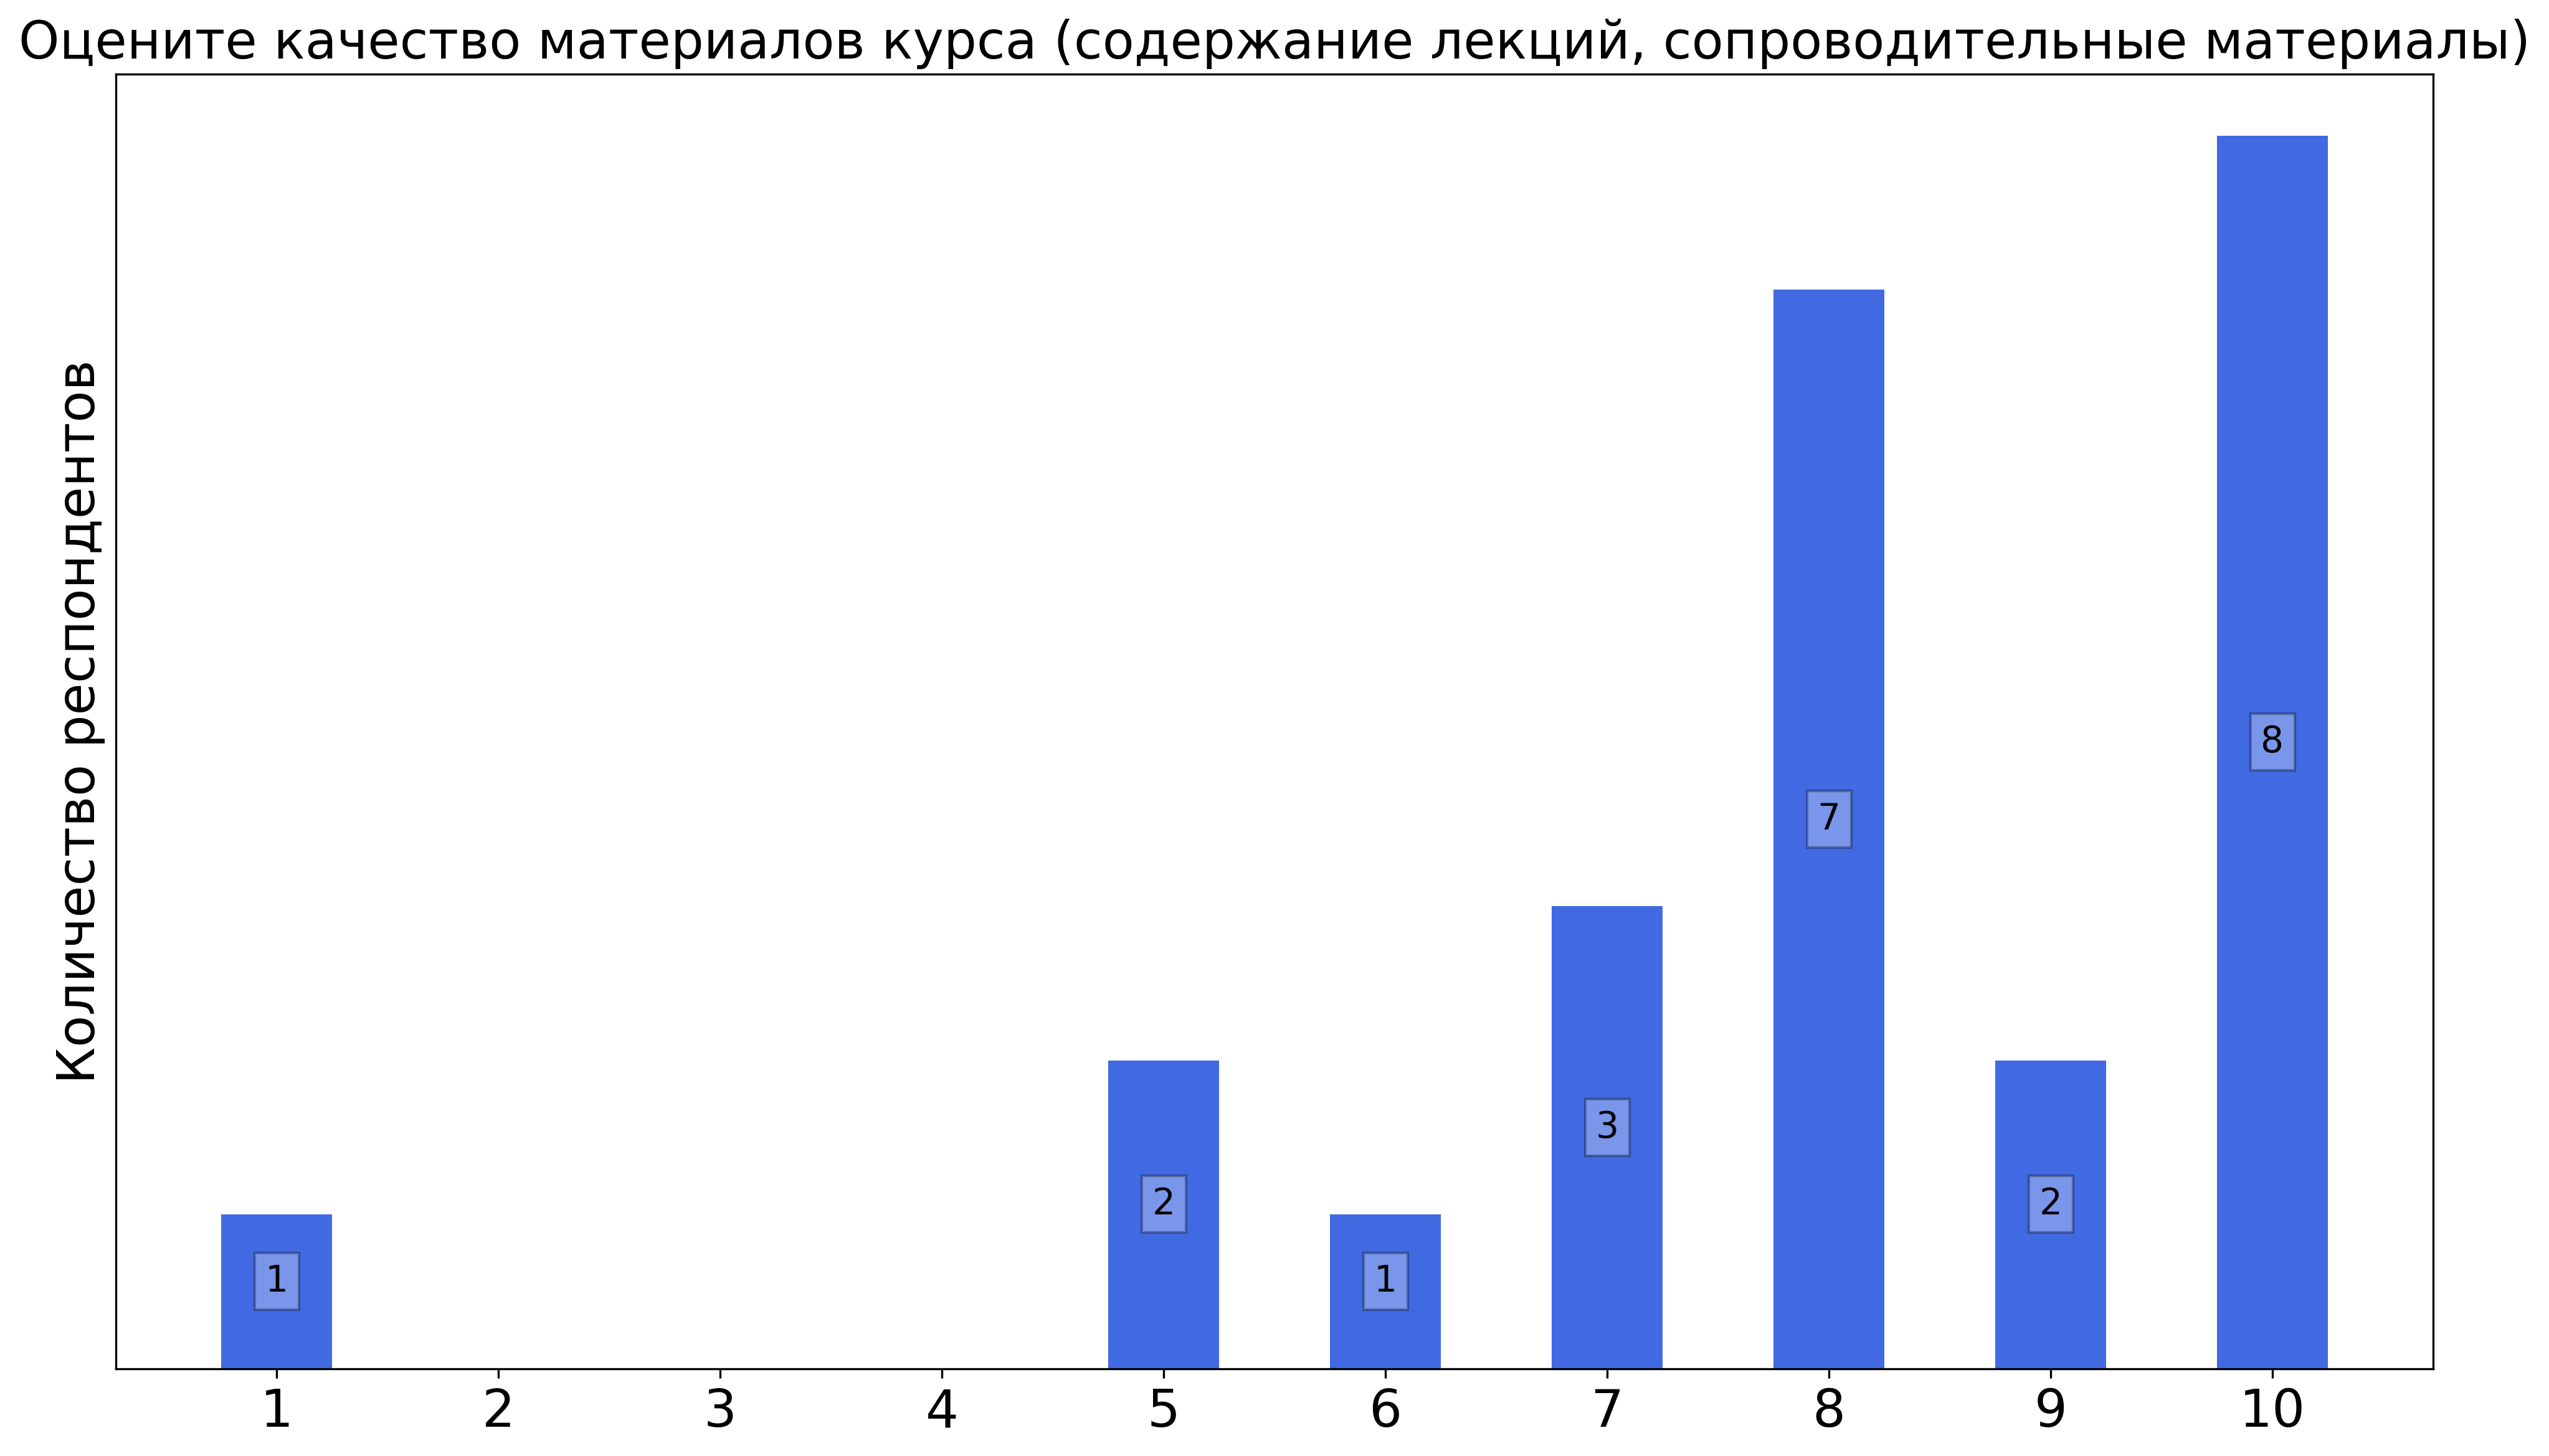
\includegraphics[width=\textwidth]{images/3 course/Теория поля/lecturer-marks-Фомичев С.В.-1.png}
			\end{subfigure}
			\begin{subfigure}[b]{0.45\textwidth}
				\centering
				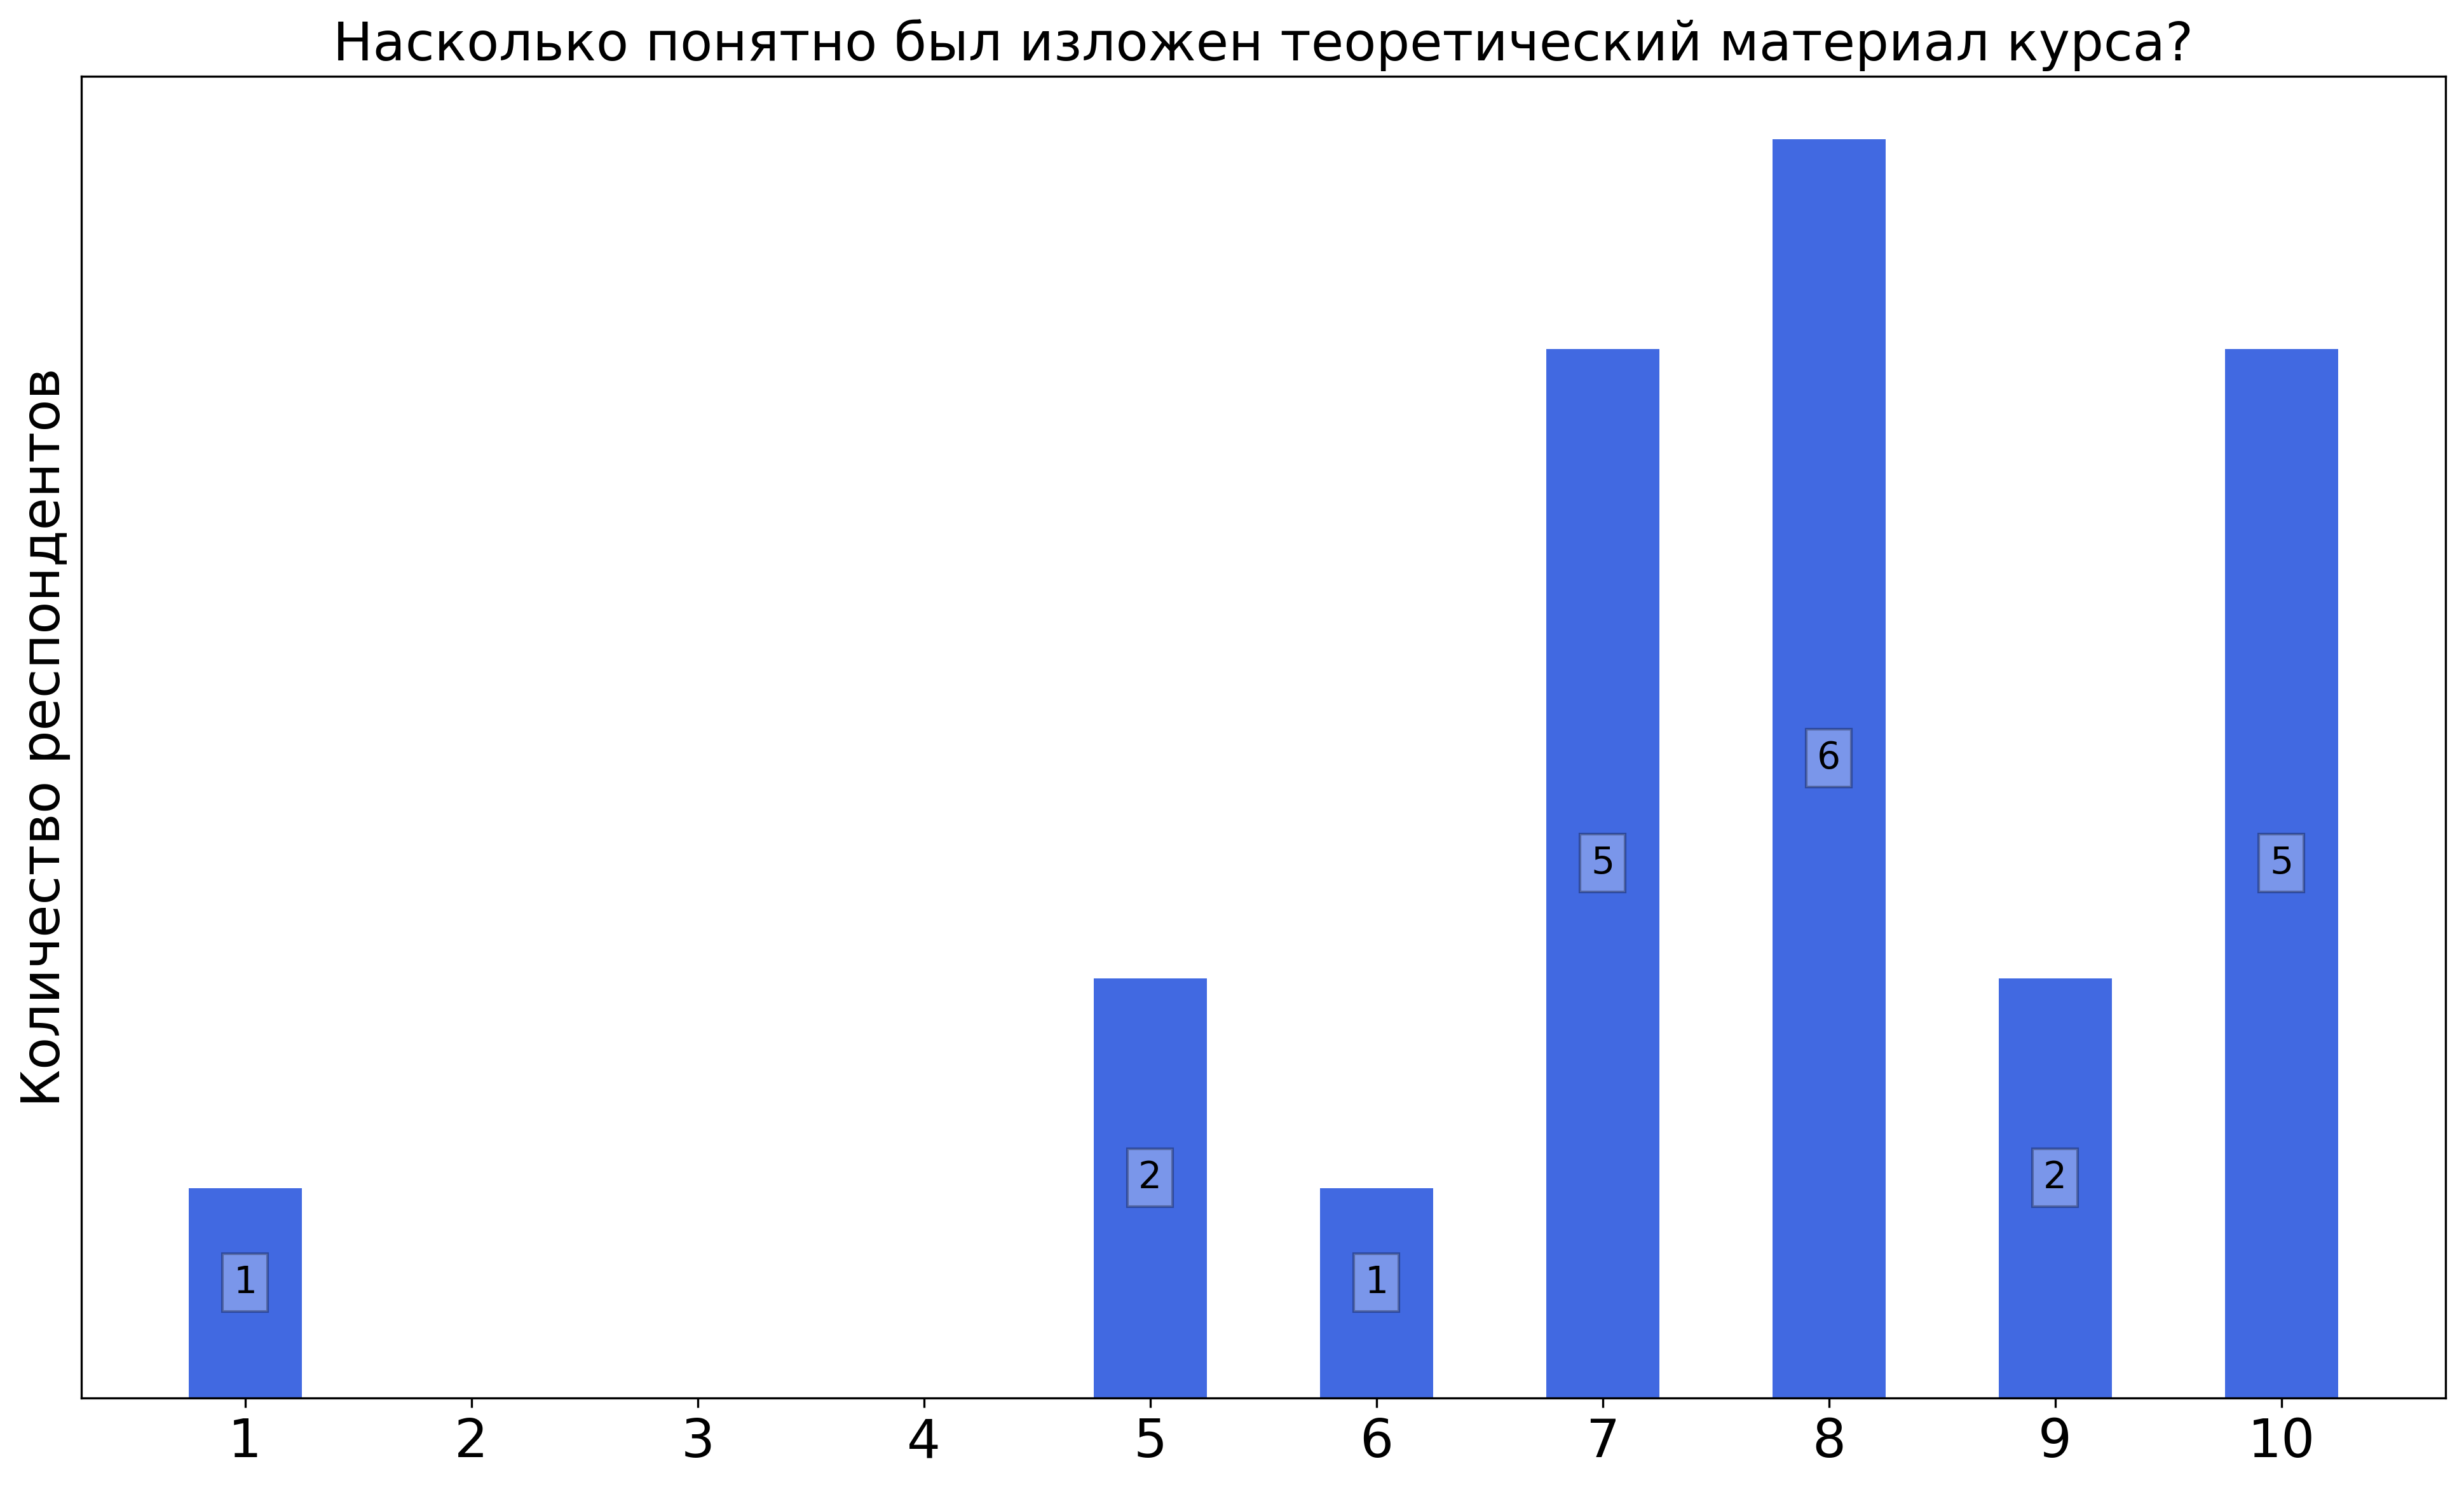
\includegraphics[width=\textwidth]{images/3 course/Теория поля/lecturer-marks-Фомичев С.В.-2.png}
			\end{subfigure}	
			\begin{subfigure}[b]{0.45\textwidth}
				\centering
				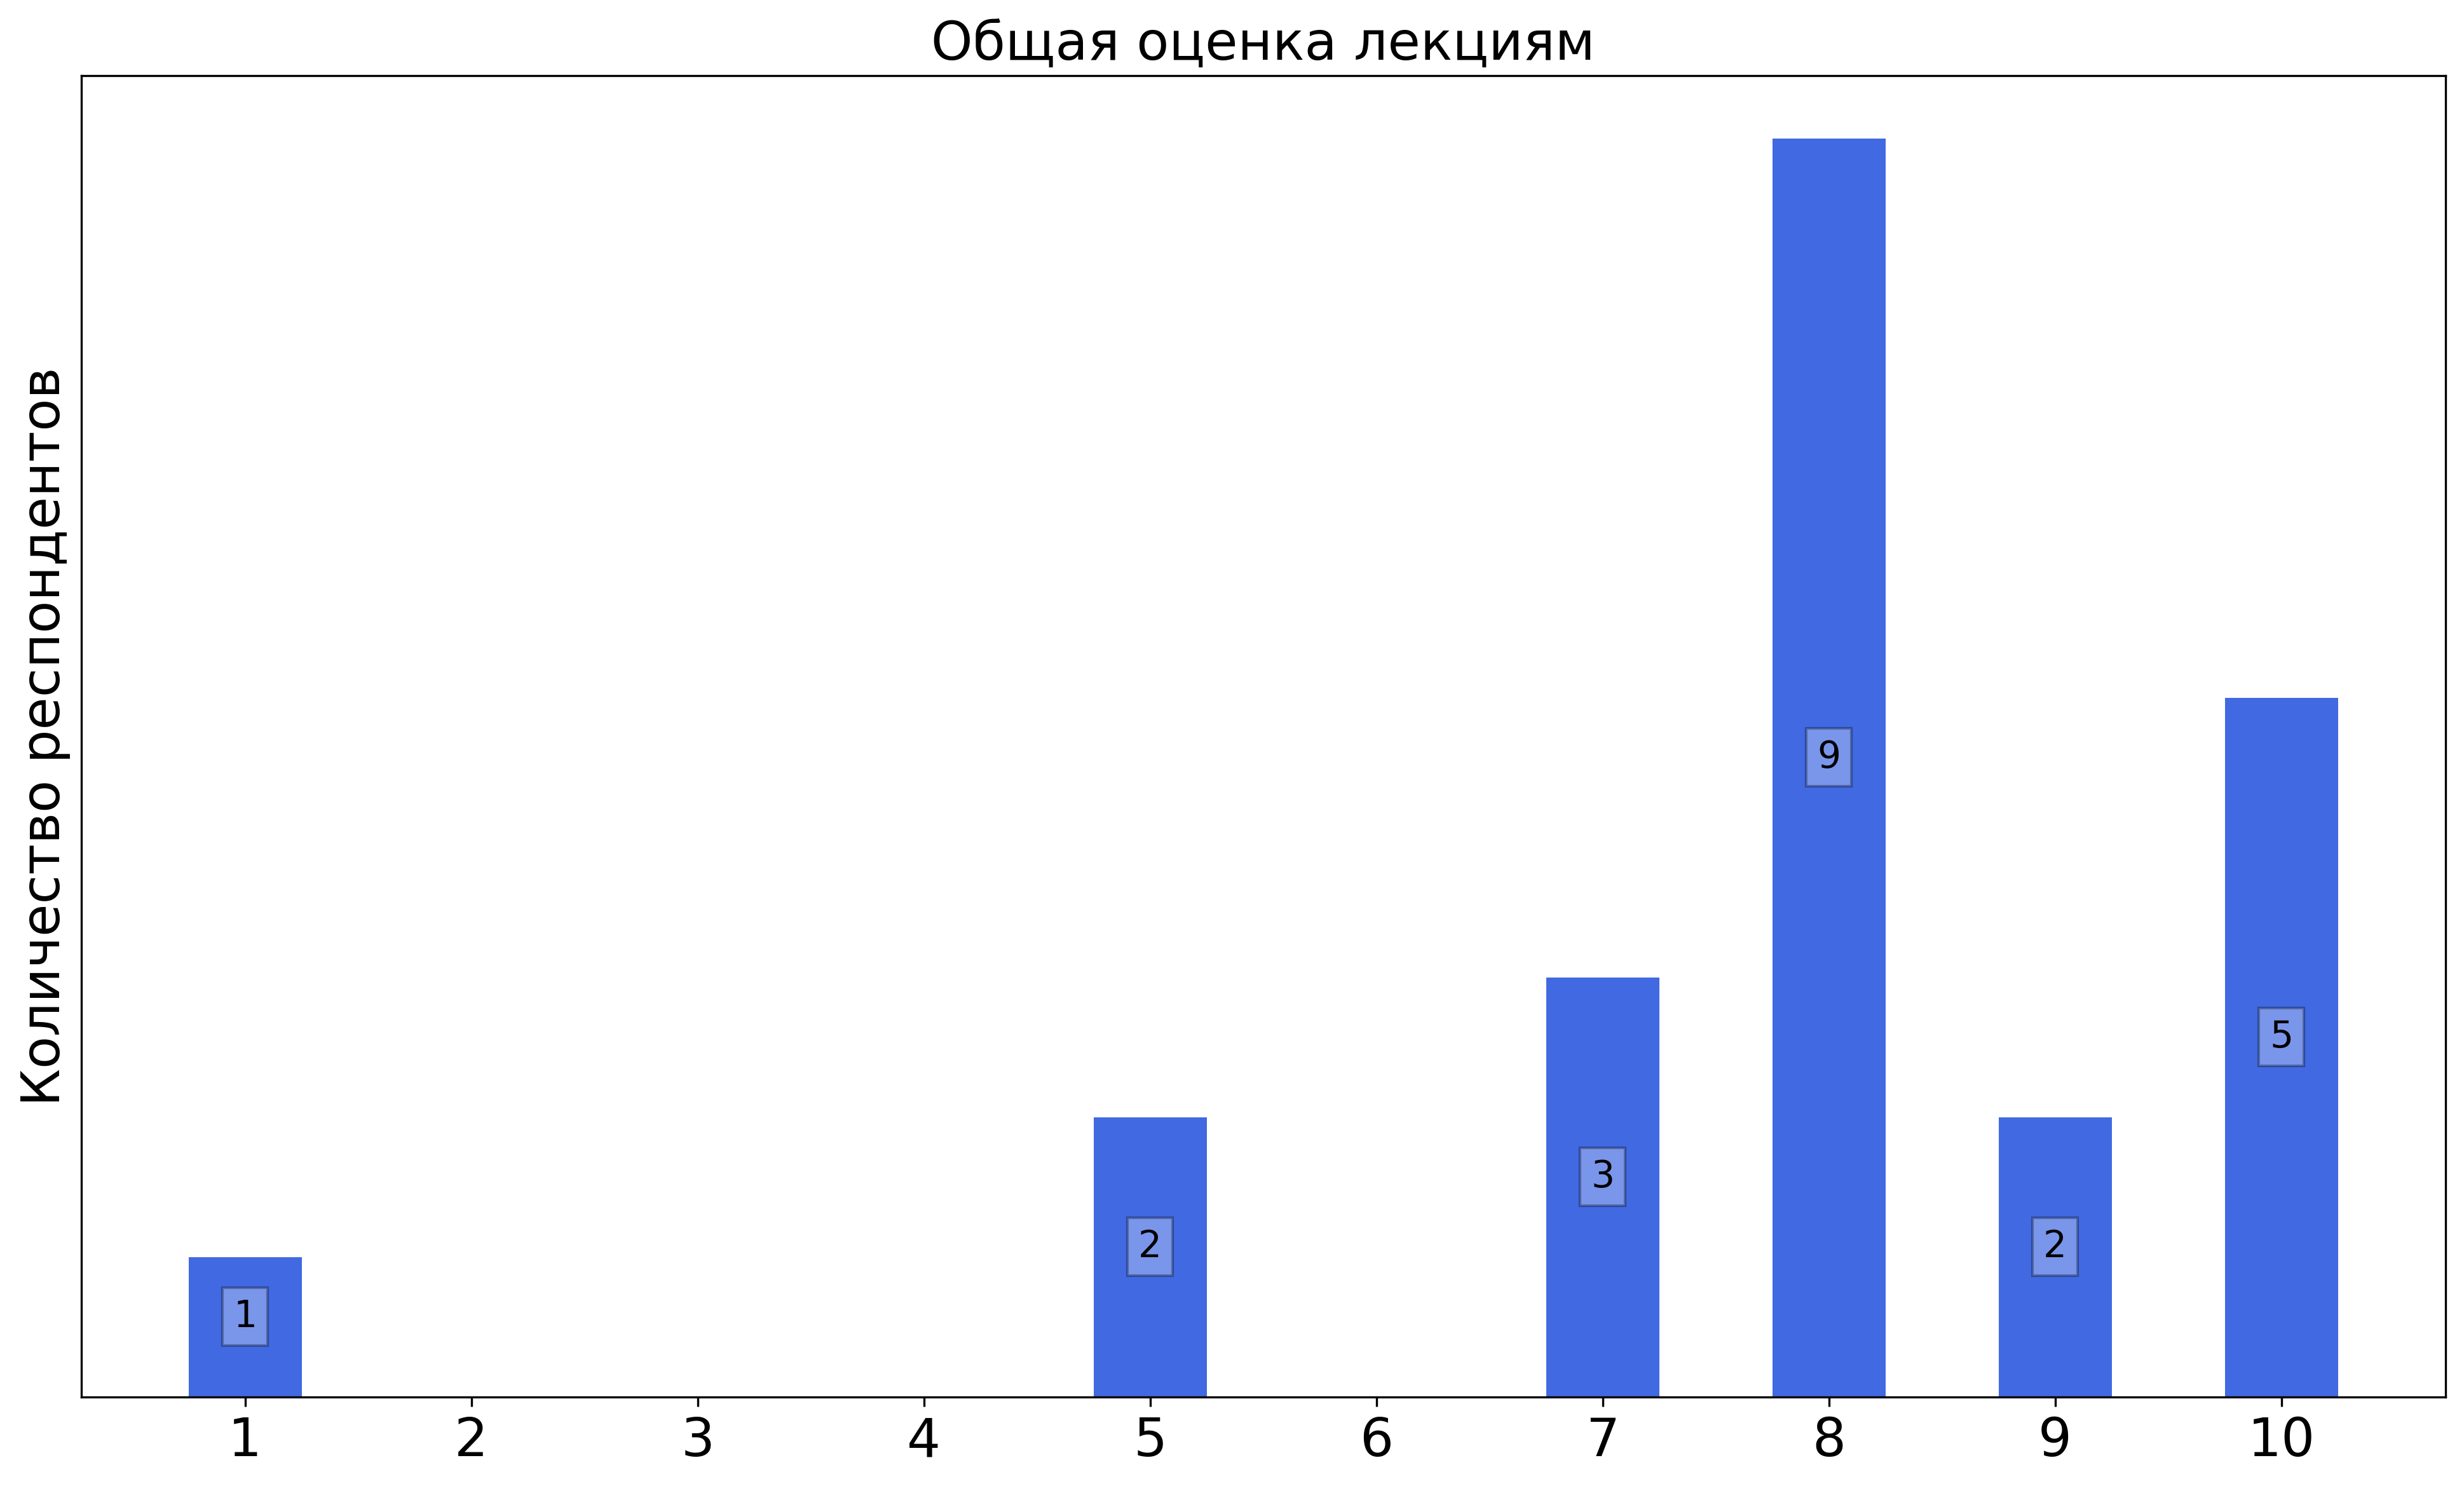
\includegraphics[width=\textwidth]{images/3 course/Теория поля/lecturer-marks-Фомичев С.В.-3.png}
			\end{subfigure}
			\caption{Оценки респондентов о качестве преподавания лекций по курсу <<Теория поля>>}
		\end{figure}

		\textbf{Комментарии студентов о лекциях\protect\footnote{сохранены оригинальные орфография и пунктуация}}
            \begin{commentbox} 
                Лектор норм. Но курс перегруженный, я втооую половину семестра просто не воспринял 
            \end{commentbox} 
        
            \begin{commentbox} 
                Лекции читаются тихо, медленно, невнятно, зато есть отличные конспекты лекций в pdf формате! 
            \end{commentbox} 
        
            \begin{commentbox} 
                Очень быстро читает. 
            \end{commentbox} 
        
            \begin{commentbox} 
                Добавить больше  физического смысла формулам  
            \end{commentbox} 
        
            \begin{commentbox} 
                Фомичев норм лектор, но его проблема в том, что он не объясняет физику процесса, а нонстопом строчит математику.  
            \end{commentbox} 
        
            \begin{commentbox} 
                Не особо ходил, но конспекты лекций очень хорошие 
            \end{commentbox} 
        
            \begin{commentbox} 
                Хороший лектор ч мощной презентацией на 300 слайдов по своему курсу, при подготовке ей активно аользовался. За самими лекциями не всегда успевал, темп высокий, но и материала в курсе много 
            \end{commentbox}  

    
    \subsubsection{Отзыв студентов о семинарах. Семинарист: Гец А.В.}
		\begin{figure}[H]
			\centering
			\begin{subfigure}[b]{0.45\textwidth}
				\centering
				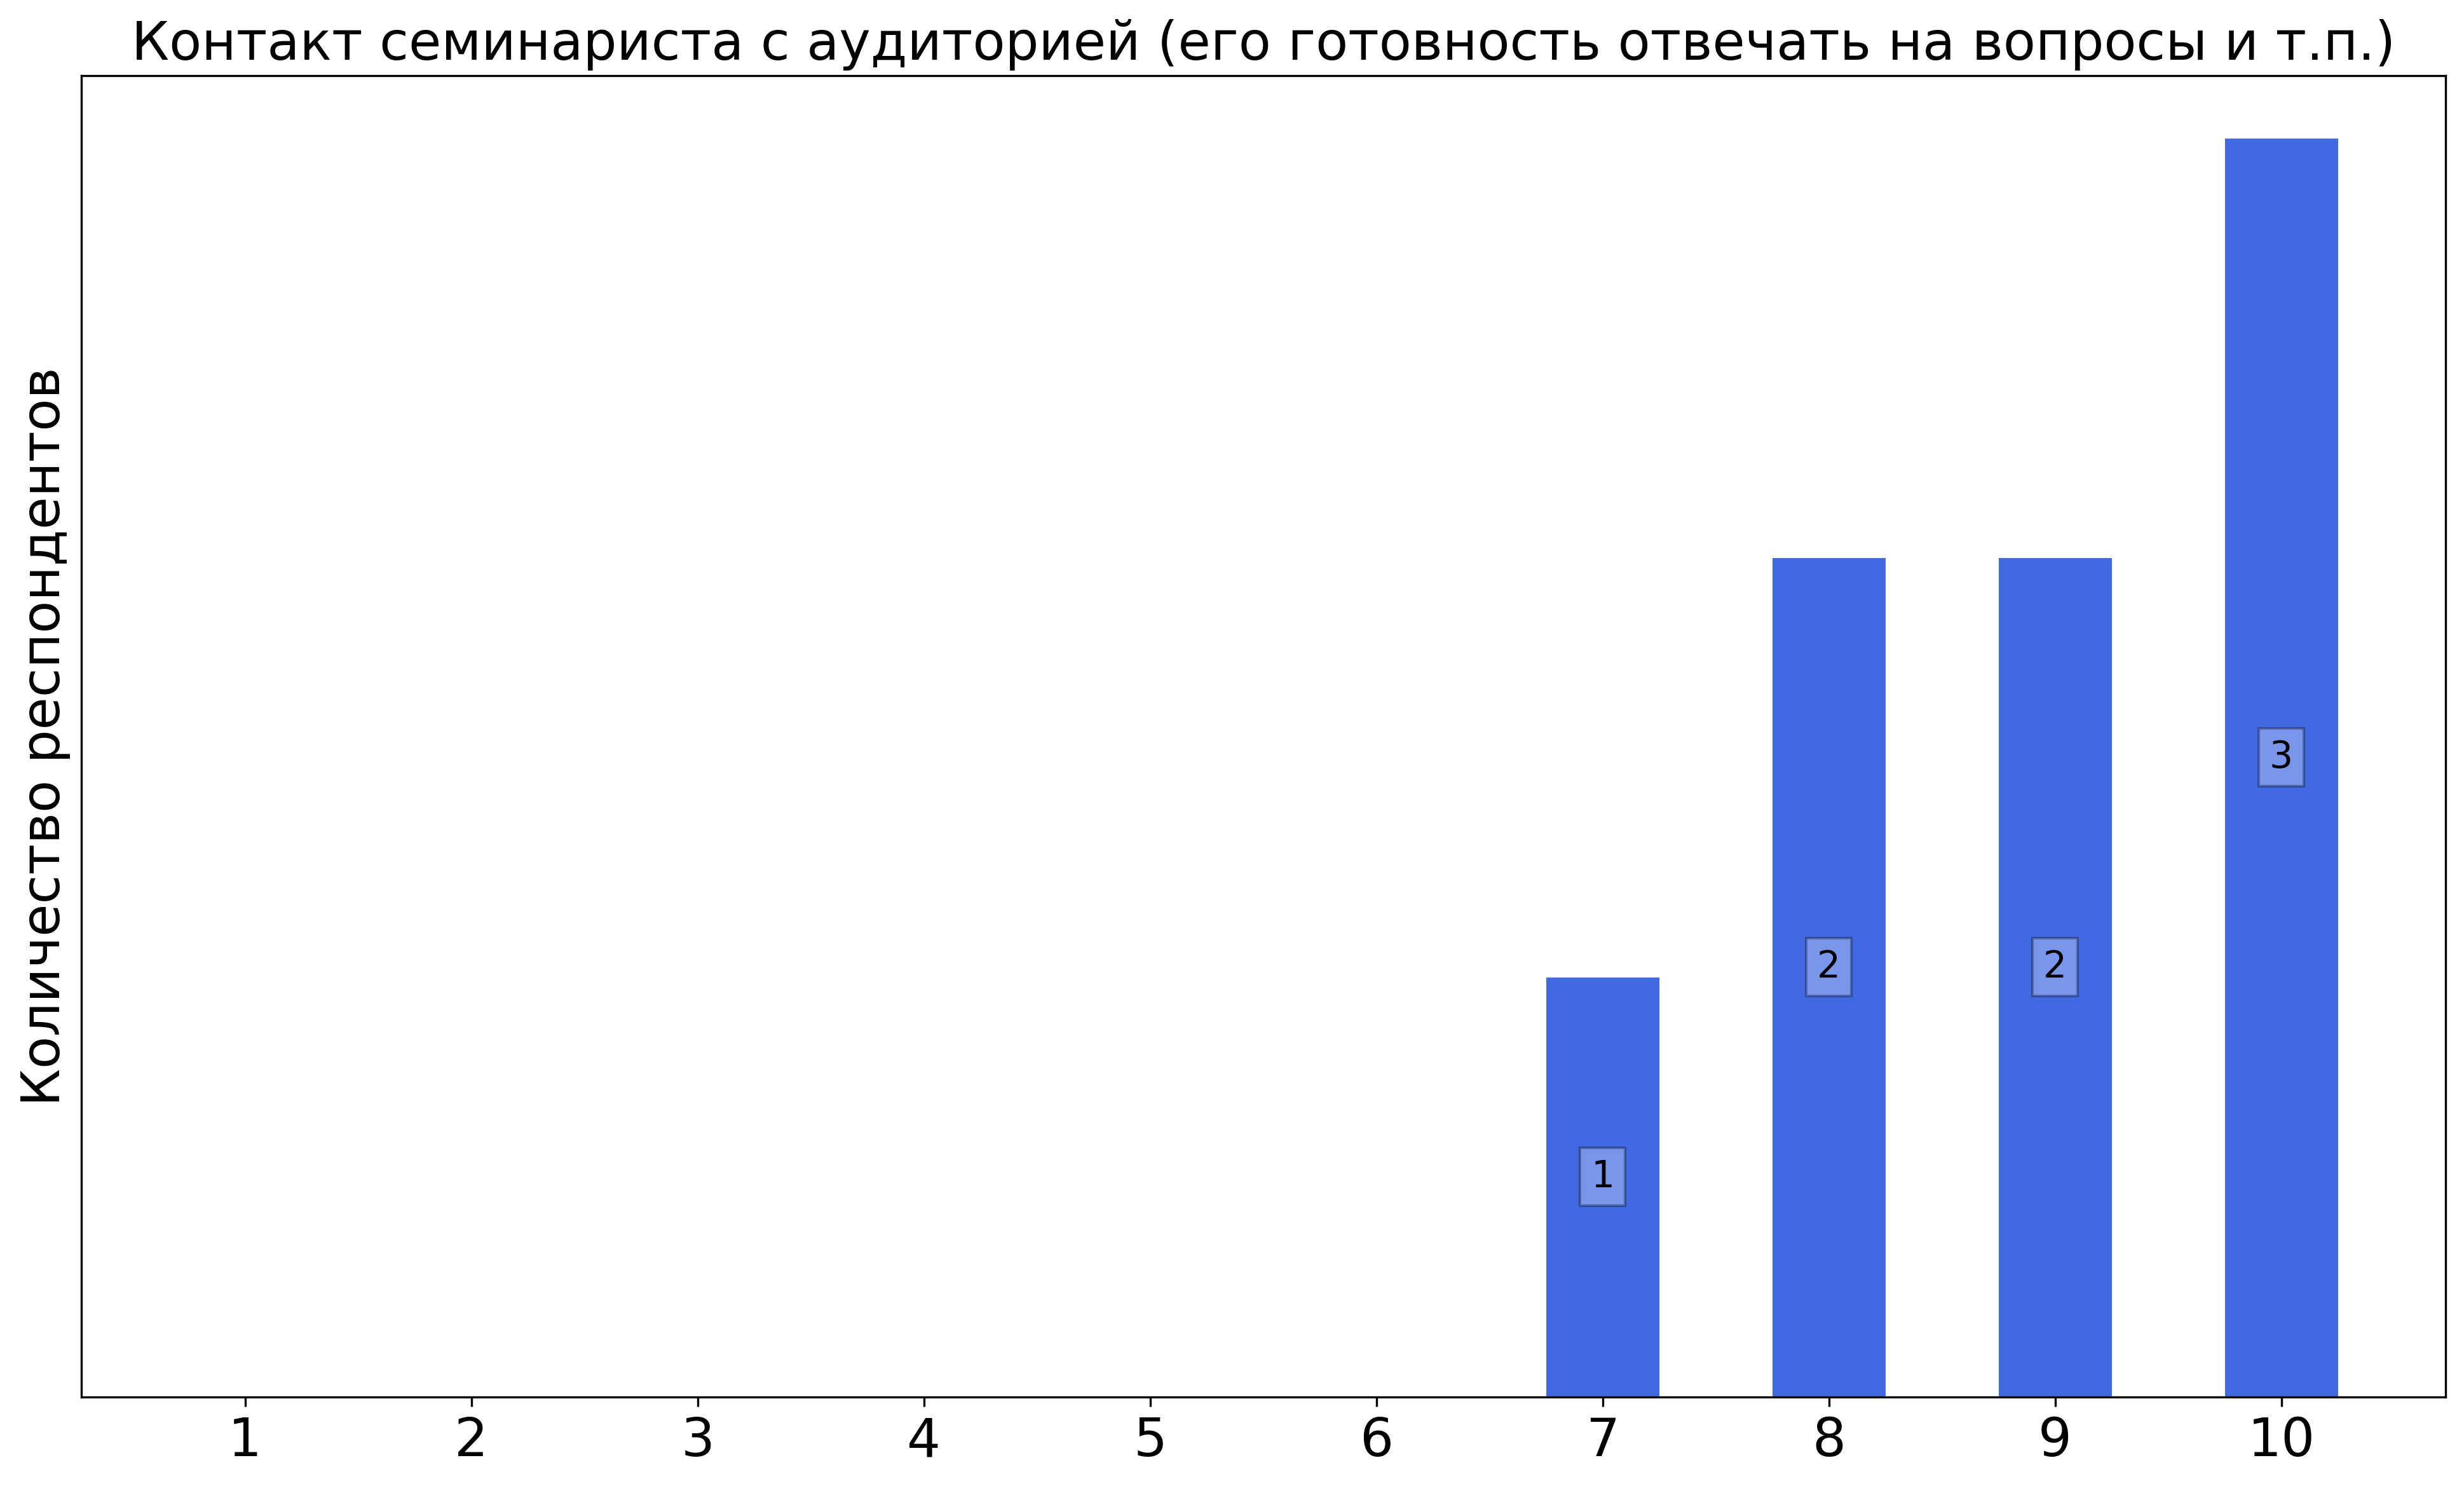
\includegraphics[width=\textwidth]{images/3 course/Теория поля/seminarists-marks-Гец А.В.-0.png}
			\end{subfigure}
			\begin{subfigure}[b]{0.45\textwidth}
				\centering
				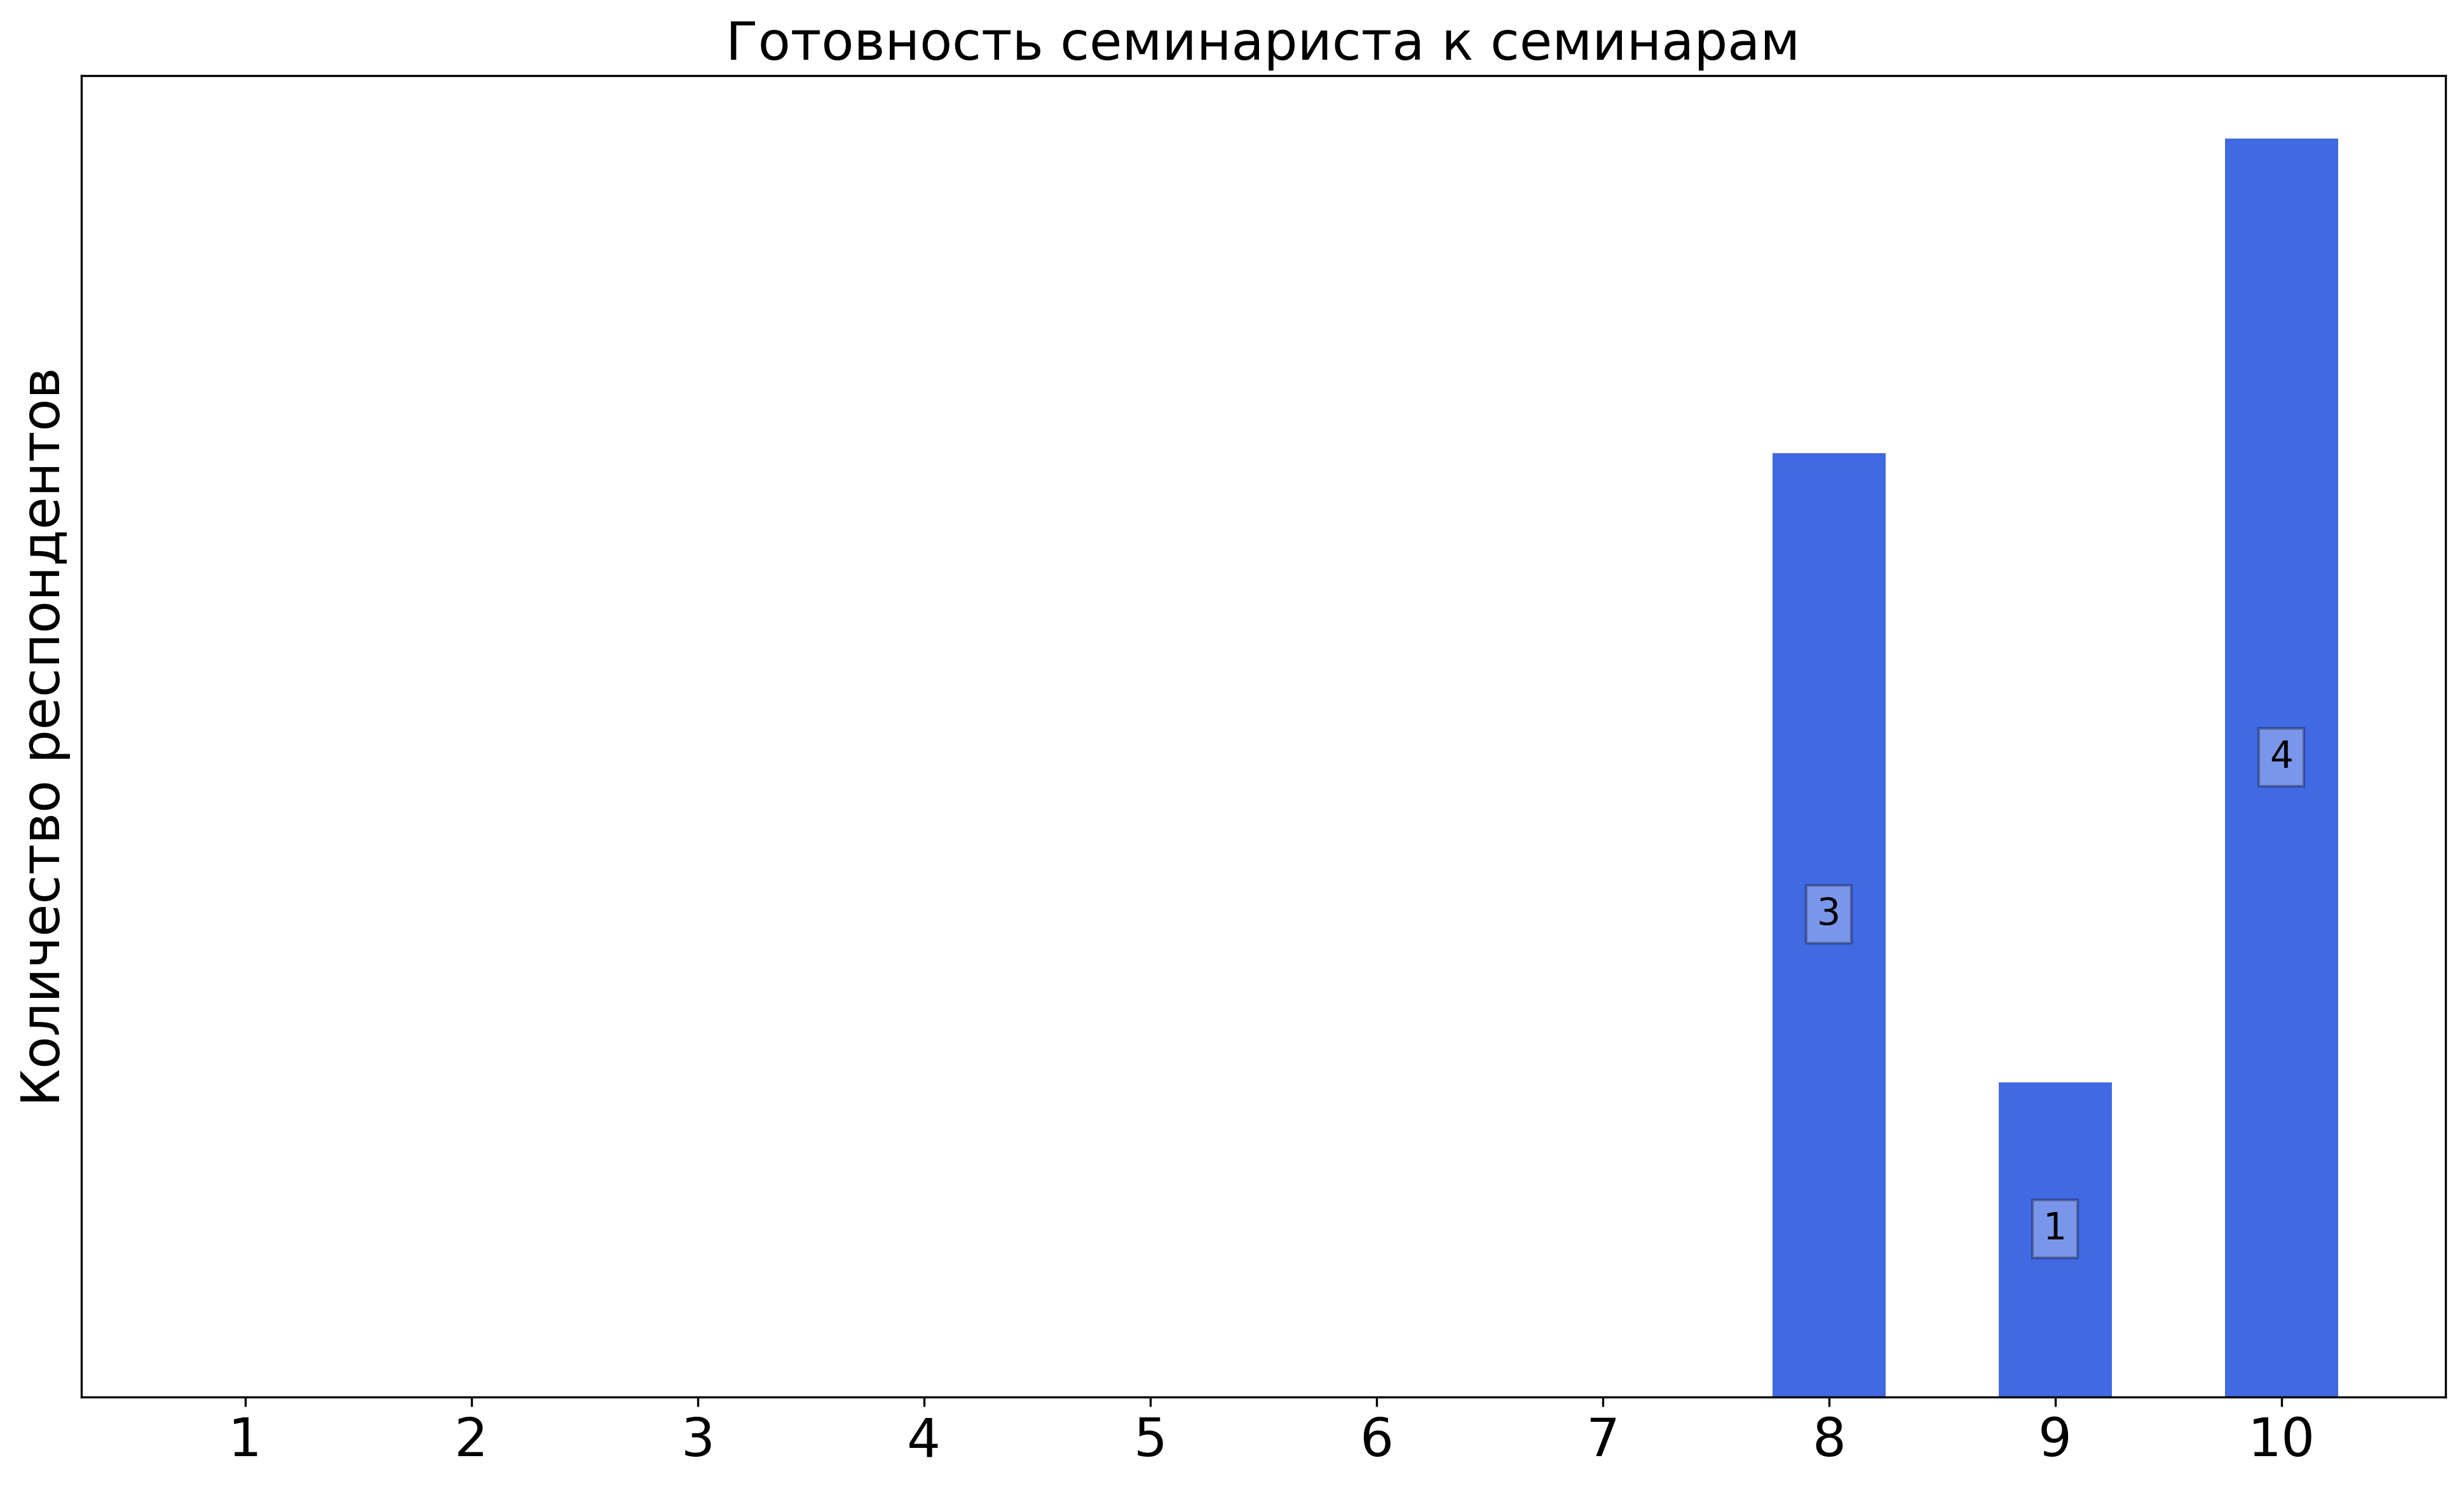
\includegraphics[width=\textwidth]{images/3 course/Теория поля/seminarists-marks-Гец А.В.-1.png}
			\end{subfigure}
			\begin{subfigure}[b]{0.45\textwidth}
				\centering
				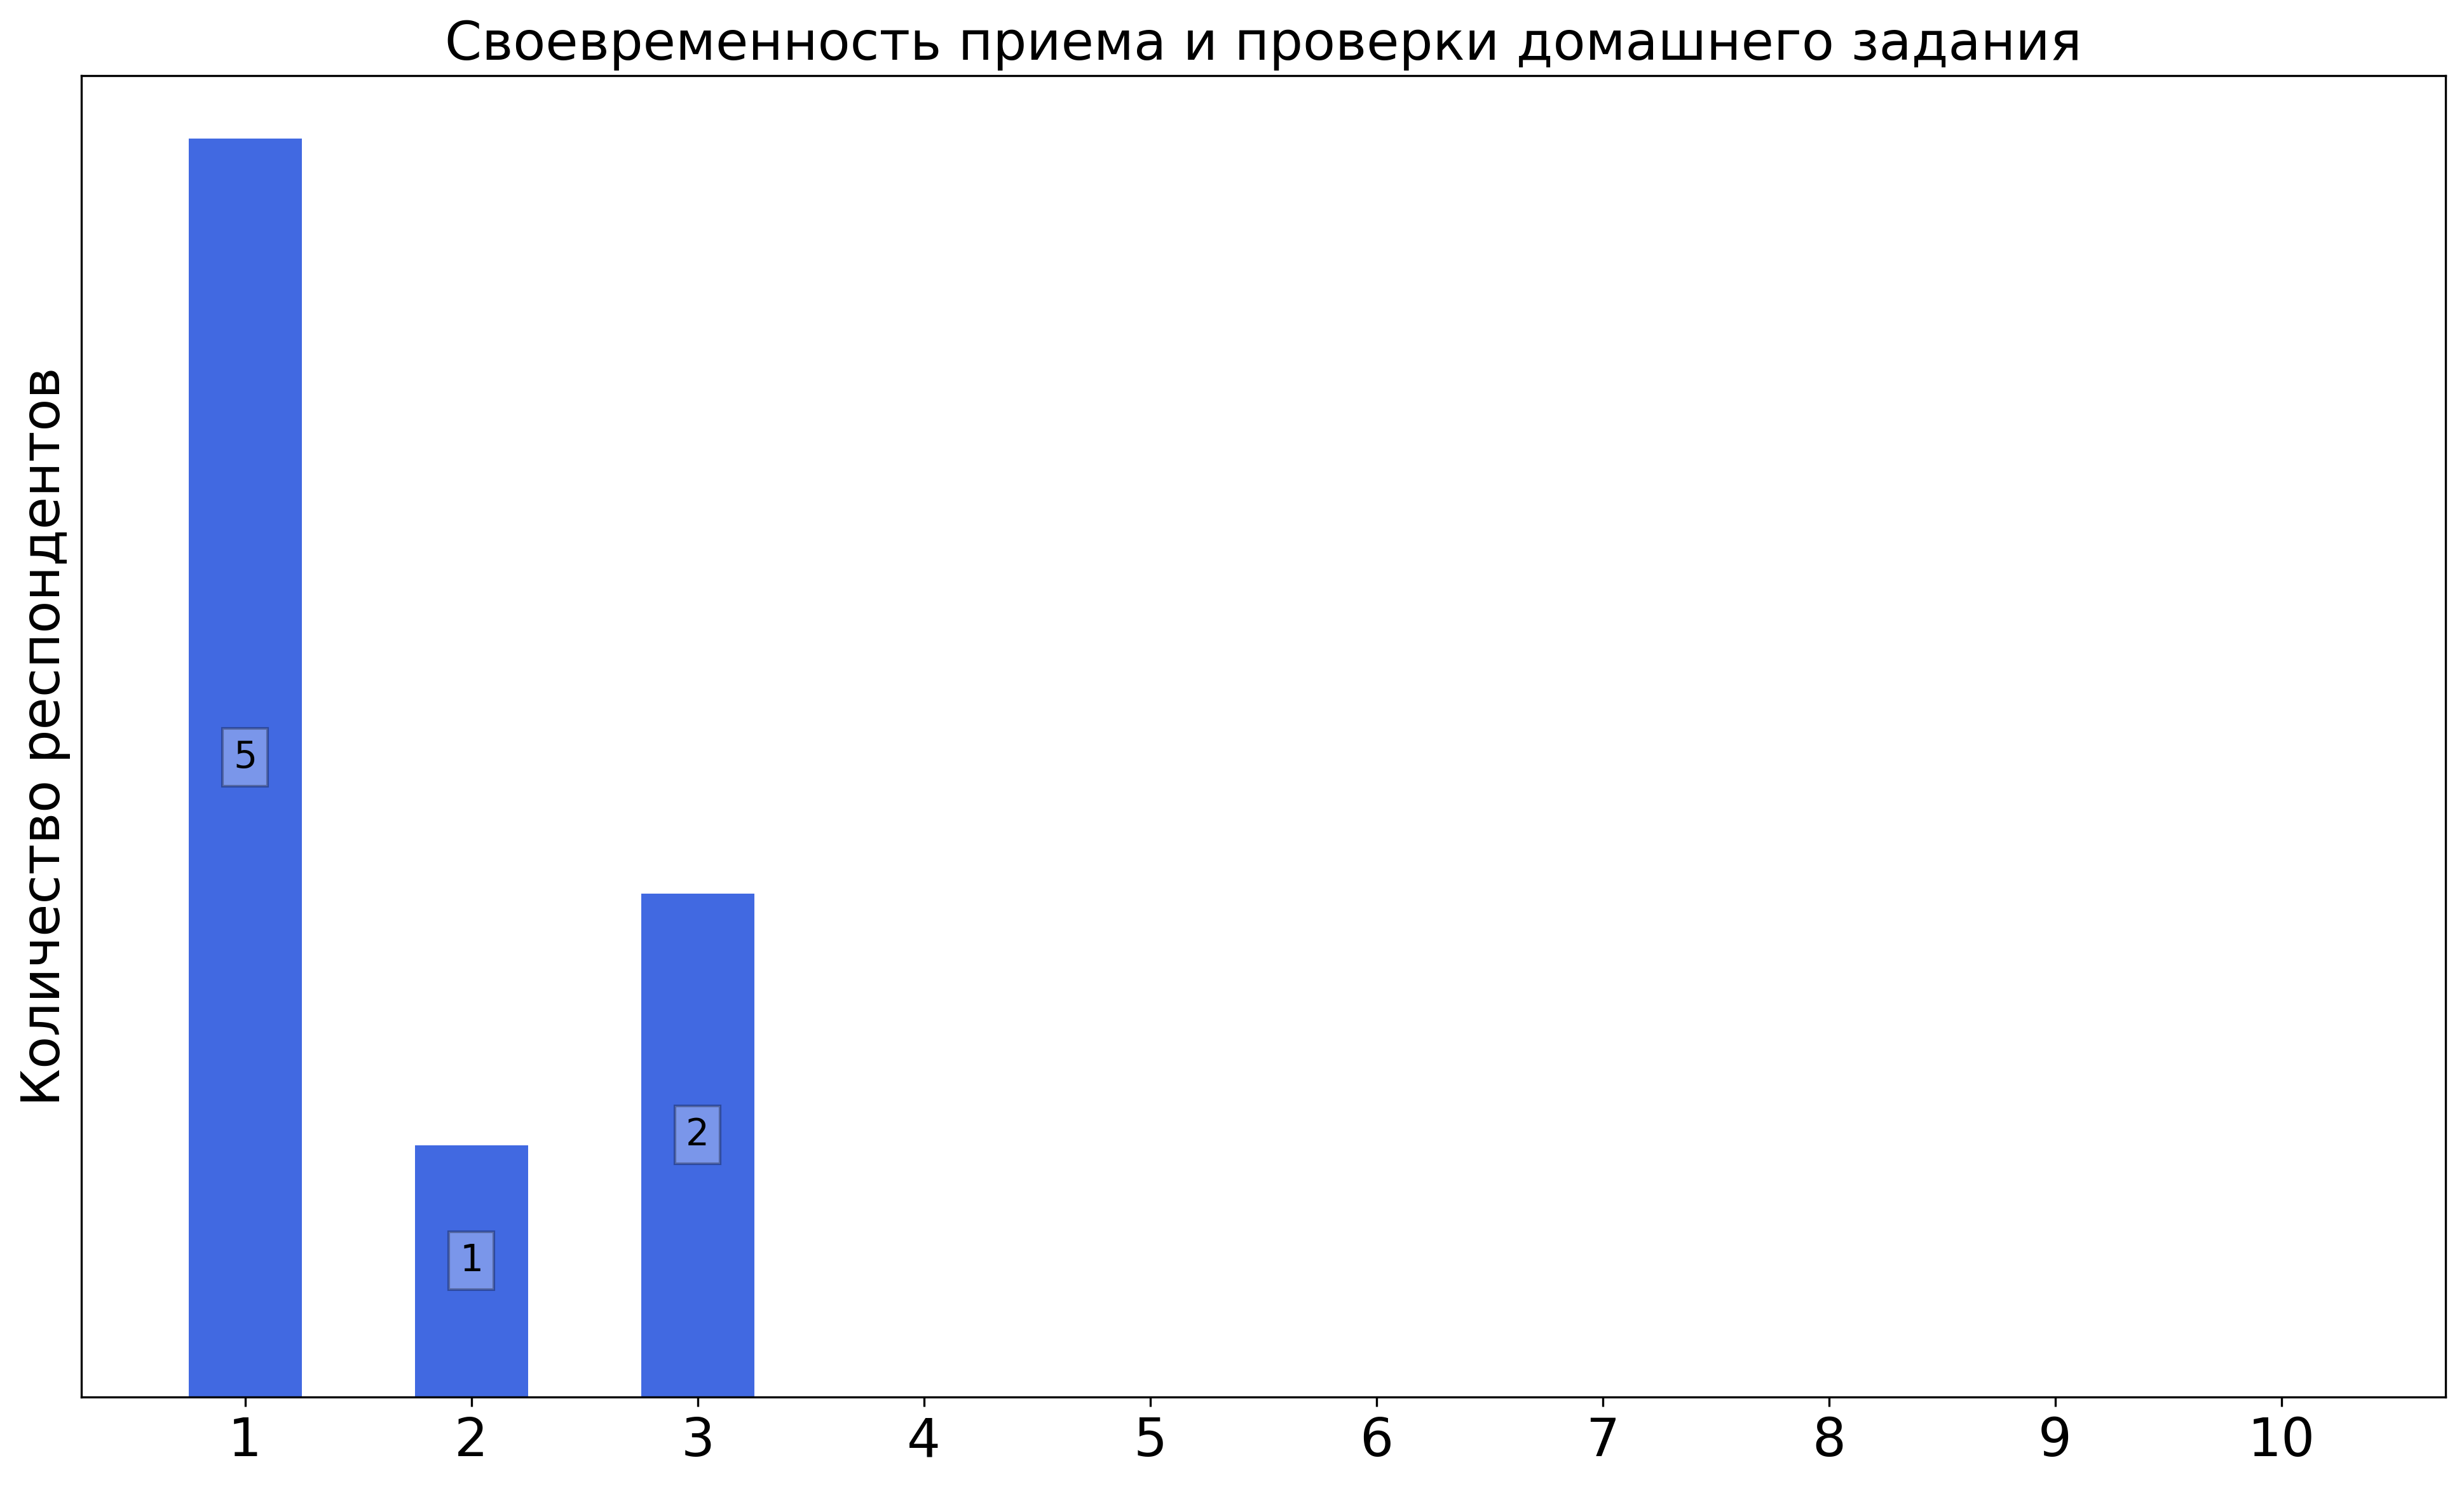
\includegraphics[width=\textwidth]{images/3 course/Теория поля/seminarists-marks-Гец А.В.-2.png}
			\end{subfigure}
			\begin{subfigure}[b]{0.45\textwidth}
				\centering
				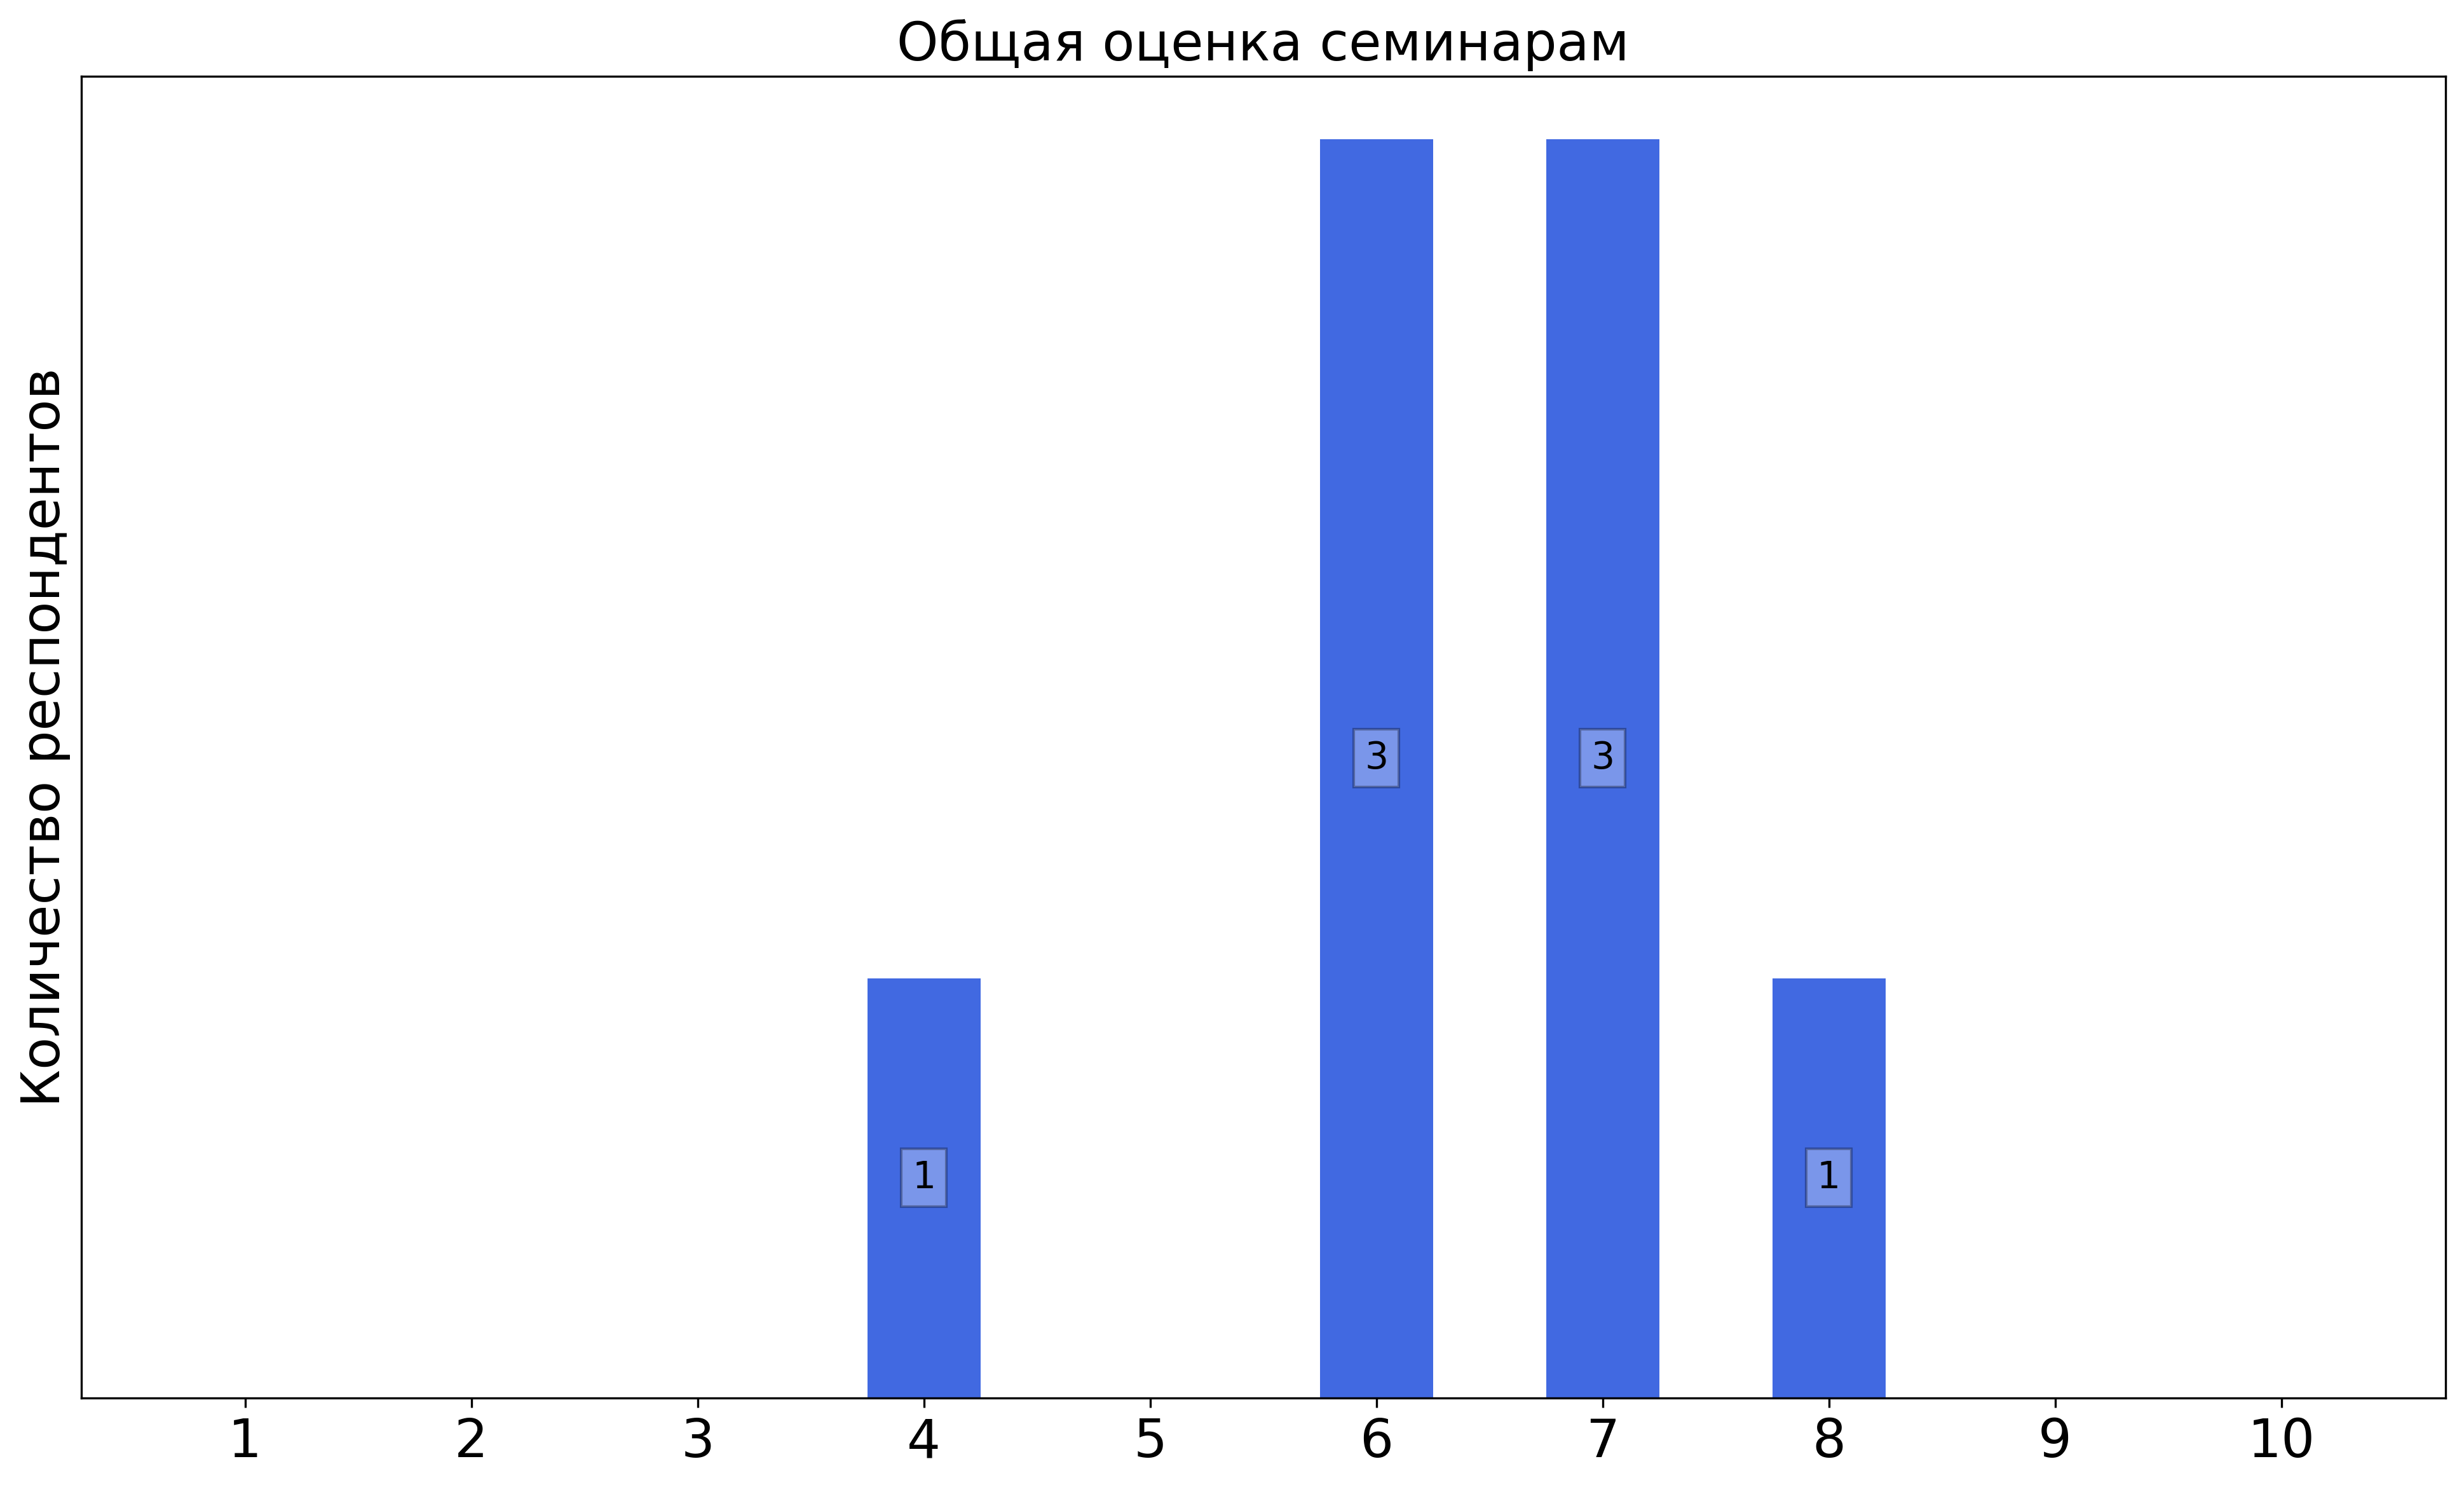
\includegraphics[width=\textwidth]{images/3 course/Теория поля/seminarists-marks-Гец А.В.-3.png}
			\end{subfigure}	
			\caption{Оценки респондентов о качестве преподавания семинаров}
		\end{figure}

		\textbf{Комментарии студентов о семинаристе\protect\footnote{сохранены оригинальные орфография и пунктуация}}
            \begin{commentbox} 
                Не было времени на сдачу дз( единственная возможность-2 окна между самим же Гецом и Климановым, что, конечно, во времена контрольных работ от обоих предметов было невыносимо) Другие дни не принимались за «неохотой ехать на физтех», а на сдачу дз уходило очень много времени. Нас не смущало количество потраченного времени, скорее отсутствие выбора слотов для сдачи. Первое дз тянулось месяц-полтора,даже больше. Второе задание начали и, собственно, закончили сдавать на зачетной неделе вместе с Климановской кр и с крГеца.  
            \end{commentbox} 
        
            \begin{commentbox} 
                Приём дз ужасен 
            \end{commentbox} 
        
            \begin{commentbox} 
                Сдачи дз очень изматывают. 7 недель на сдачу первого дз, сдача второго проводилась в два этапа полностью на зачётной неделе. Если бы группа не провела разговор с семенаристом о том, что мы уже не успеваем сдавать дз в связи с кр по сетям и его же кр по теорполу, то возможно сдача проводилась бы прямо на экзамене либо её бы вообще не было. Иногда было не понятно, что от тебя хочет преподаватель на сдачи (были фразы по типу: "Вы вроде правильные вещи говорите, но что-то вокруг да около сути, переформулируйте". В итоге в течение 4 недели мне было не понятно, что нужно сказать, хотя я спрашивал). Обычно начать сдавать успевают 4-5 человек, остальные могут уйти ни с чем. При этом сами семинары классные, материал объясняется понятно, разбираются задачи из дз 
            \end{commentbox} 
        
            \begin{commentbox} 
                На семинарах объясняет хорошо, благодаря семинарам я неплохо научилась решать задачи, но вот сдача задания проходит слишком долго и не всегда понятные требования. 
            \end{commentbox} 
        
            \begin{commentbox} 
                Сдачи задания затягивались, не по вине студентов. А конкретных критериев оценивания не было. Сдача первого задания проводилась вплоть до декабря, хотя срок его сдачи гораздо раньше, причём все приходили с выполненым заднием на почти все сдачи. Из-за этого сдача второго перешла аж на зачётную неделю в дни когда проводились большие потоковые контрольные, что не предусмотренно программой курса. 
            \end{commentbox} 
        
            \begin{commentbox} 
                Гец Артем Викторович слишком много задает вопросов одному студенту пока остальные ждут,тем самым другим не хаватает времениН.е равномерно распределяет сдачи заданий, занимает под сдачи окна, иногда пары , из-за этого сдачи копятся под конец семестра, и ближе к зачетной недели он принимает у всех лишь бы поставить оценку, чаще заниженную. Семинары рассказывает хорошо, очень хорошо разбирается в материале. Приятно и интересно слушать . 
            \end{commentbox} 
        
            \begin{commentbox} 
                Я не хочу сдавать первое задание в декабре...
                Второе вообще сдавалось на зачётной неделе и ему было ... на загруз по другим предметам 
            \end{commentbox}


    \subsubsection{Отзыв студентов о семинарах. Семинарист: Девизорова Ж.А.}
        \begin{figure}[H]
            \centering
            \begin{subfigure}[b]{0.45\textwidth}
                \centering
                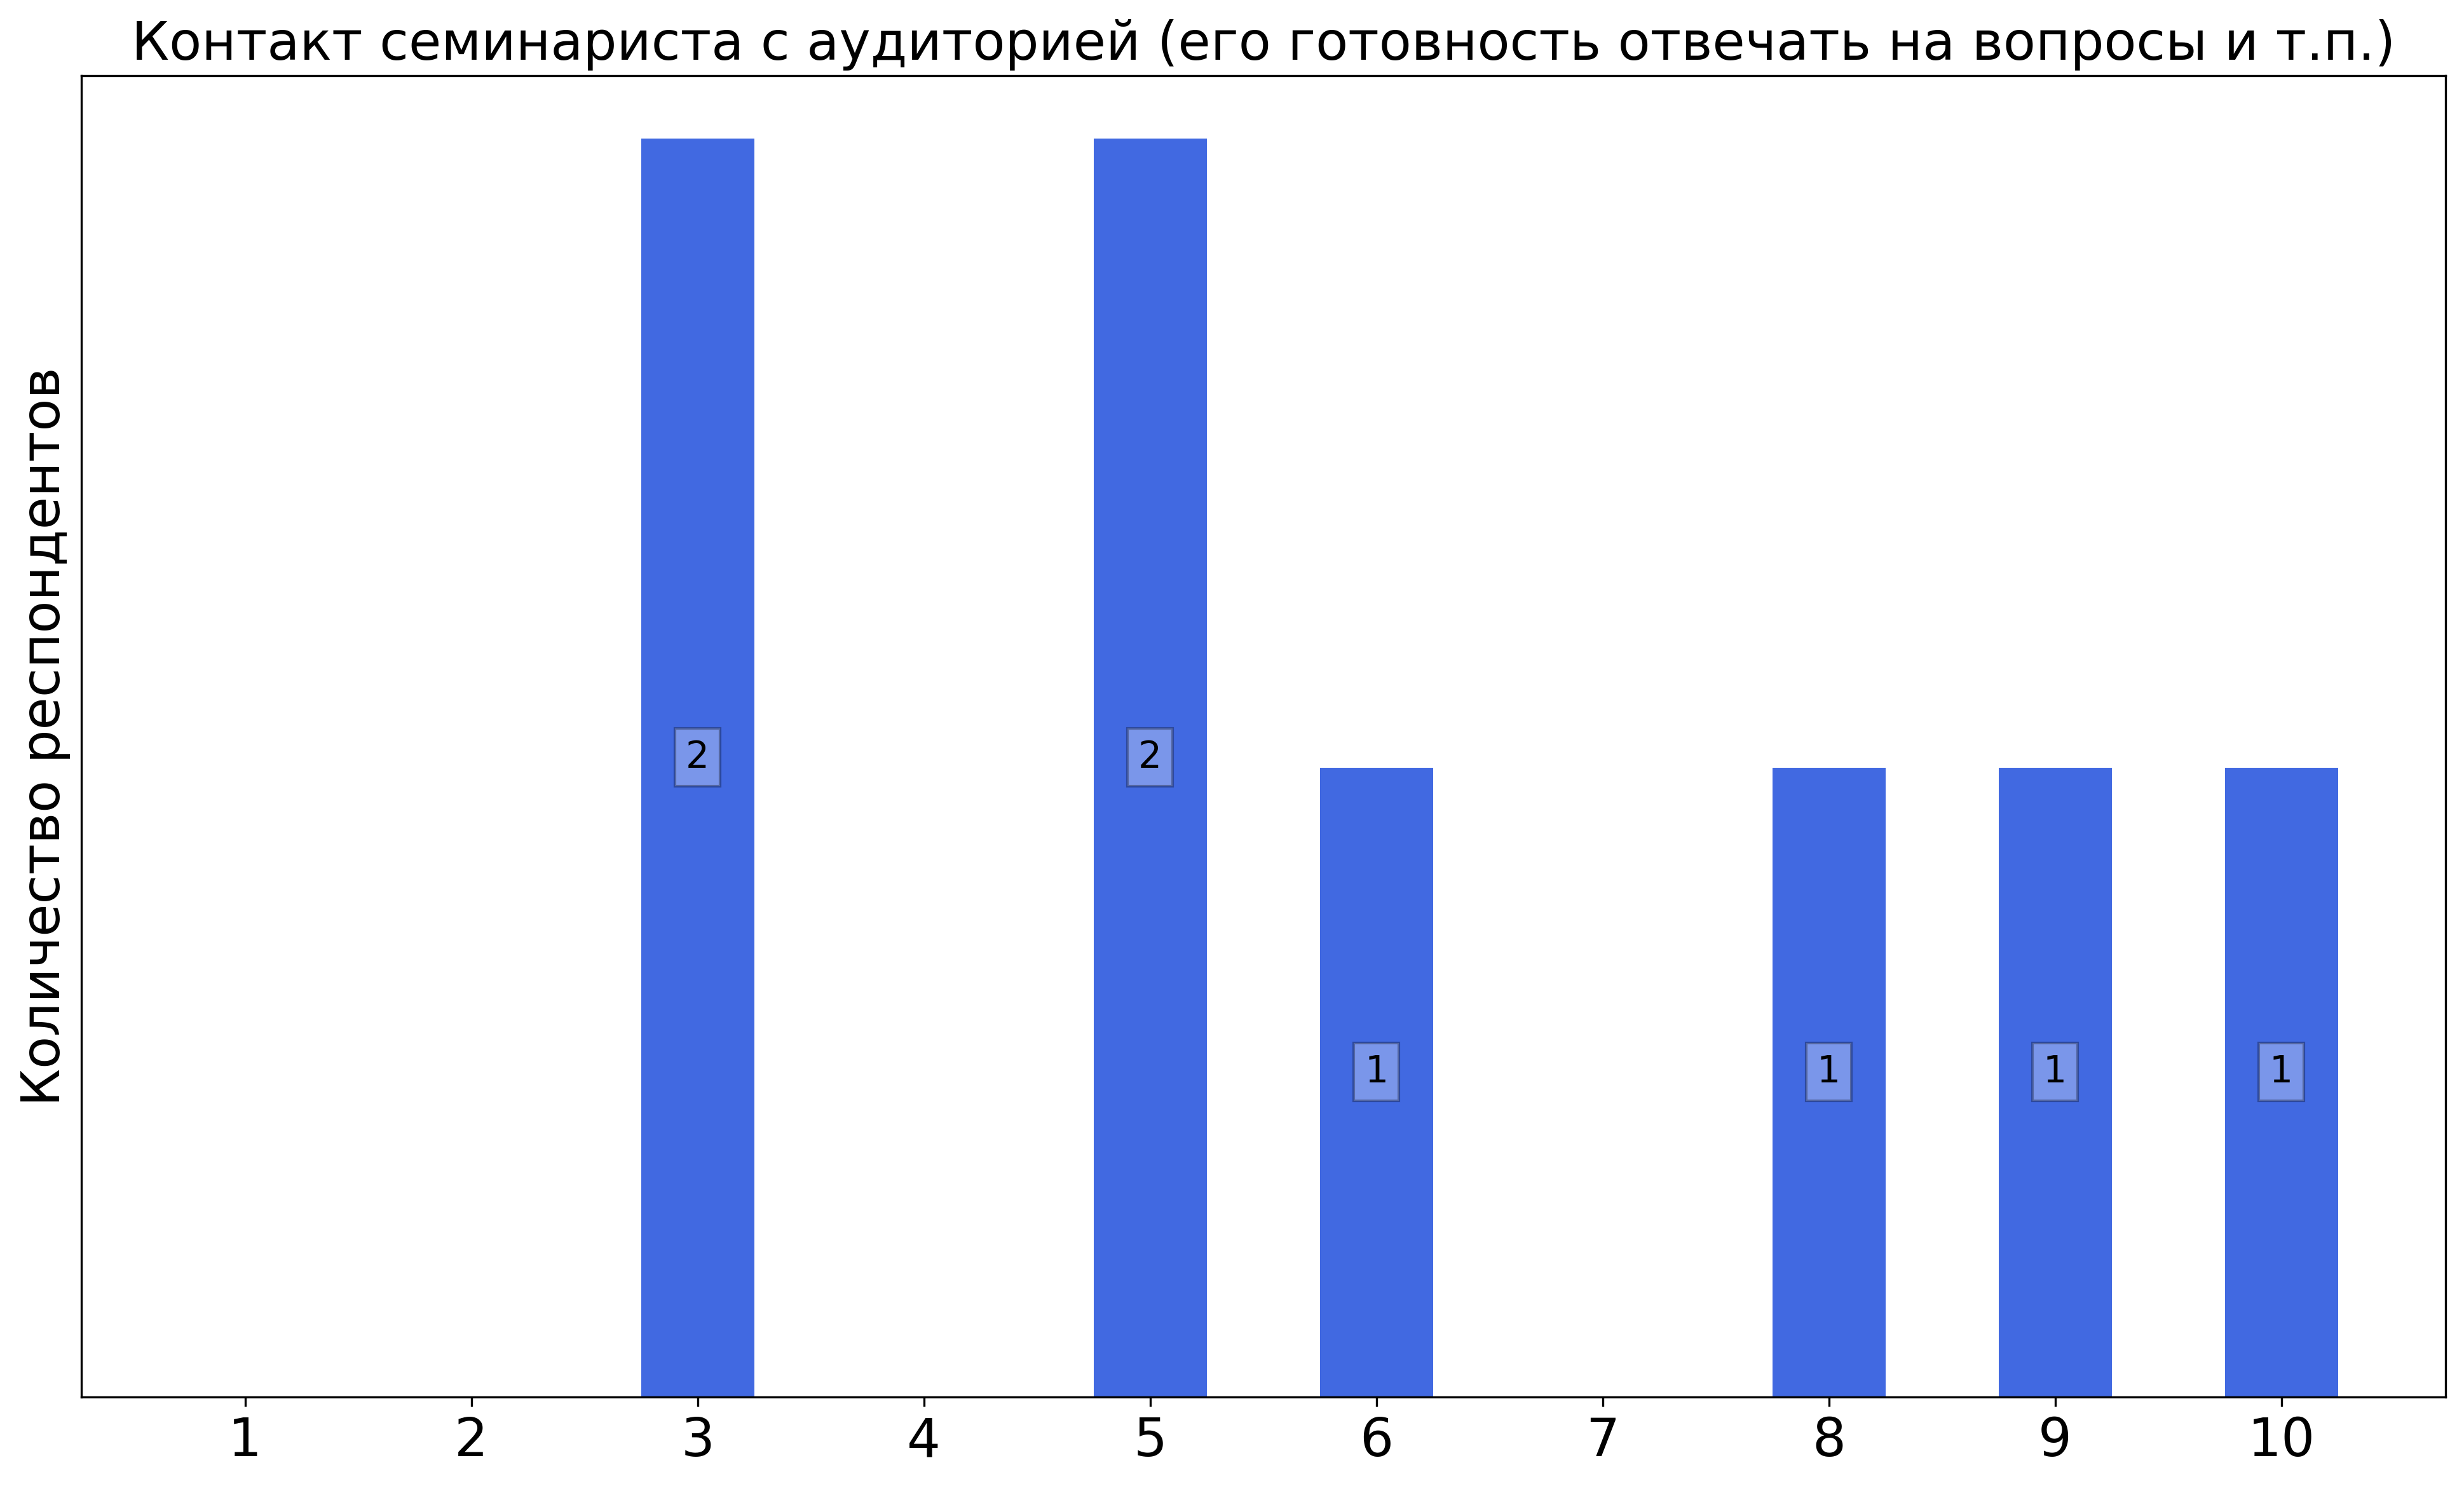
\includegraphics[width=\textwidth]{images/3 course/Теория поля/seminarists-marks-Девизорова Ж.А.-0.png}
            \end{subfigure}
            \begin{subfigure}[b]{0.45\textwidth}
                \centering
                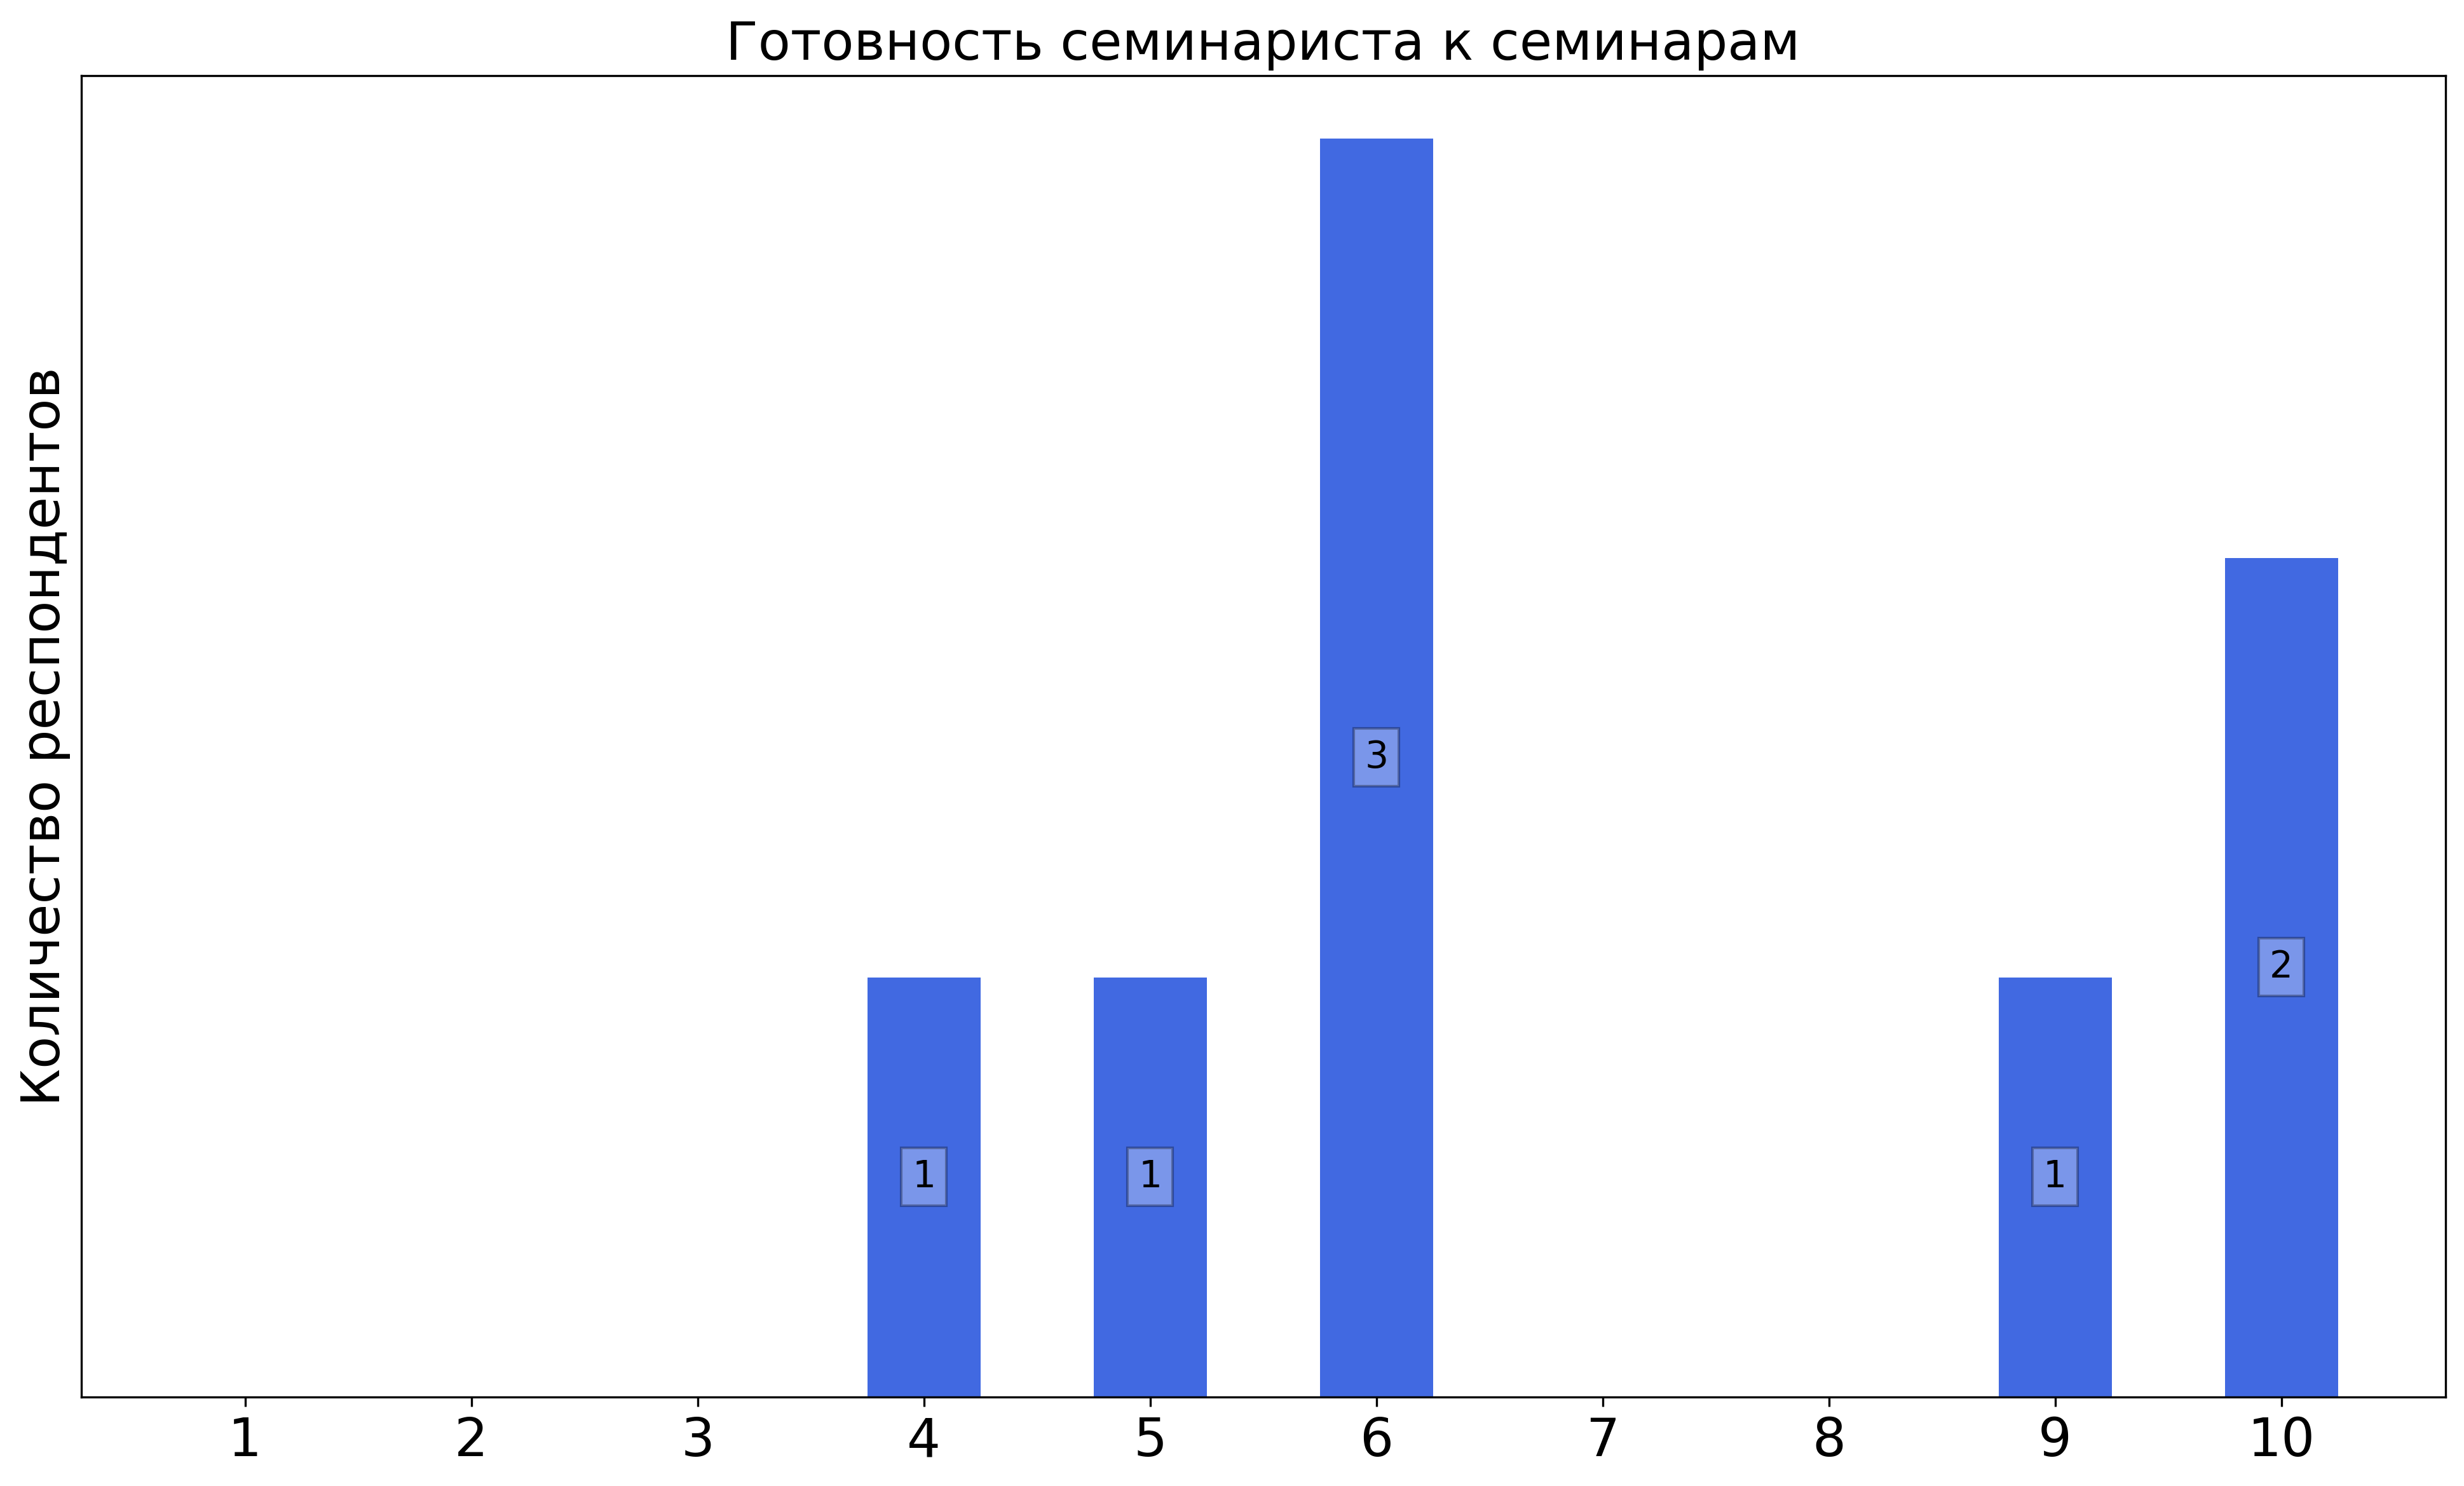
\includegraphics[width=\textwidth]{images/3 course/Теория поля/seminarists-marks-Девизорова Ж.А.-1.png}
            \end{subfigure}
            \begin{subfigure}[b]{0.45\textwidth}
                \centering
                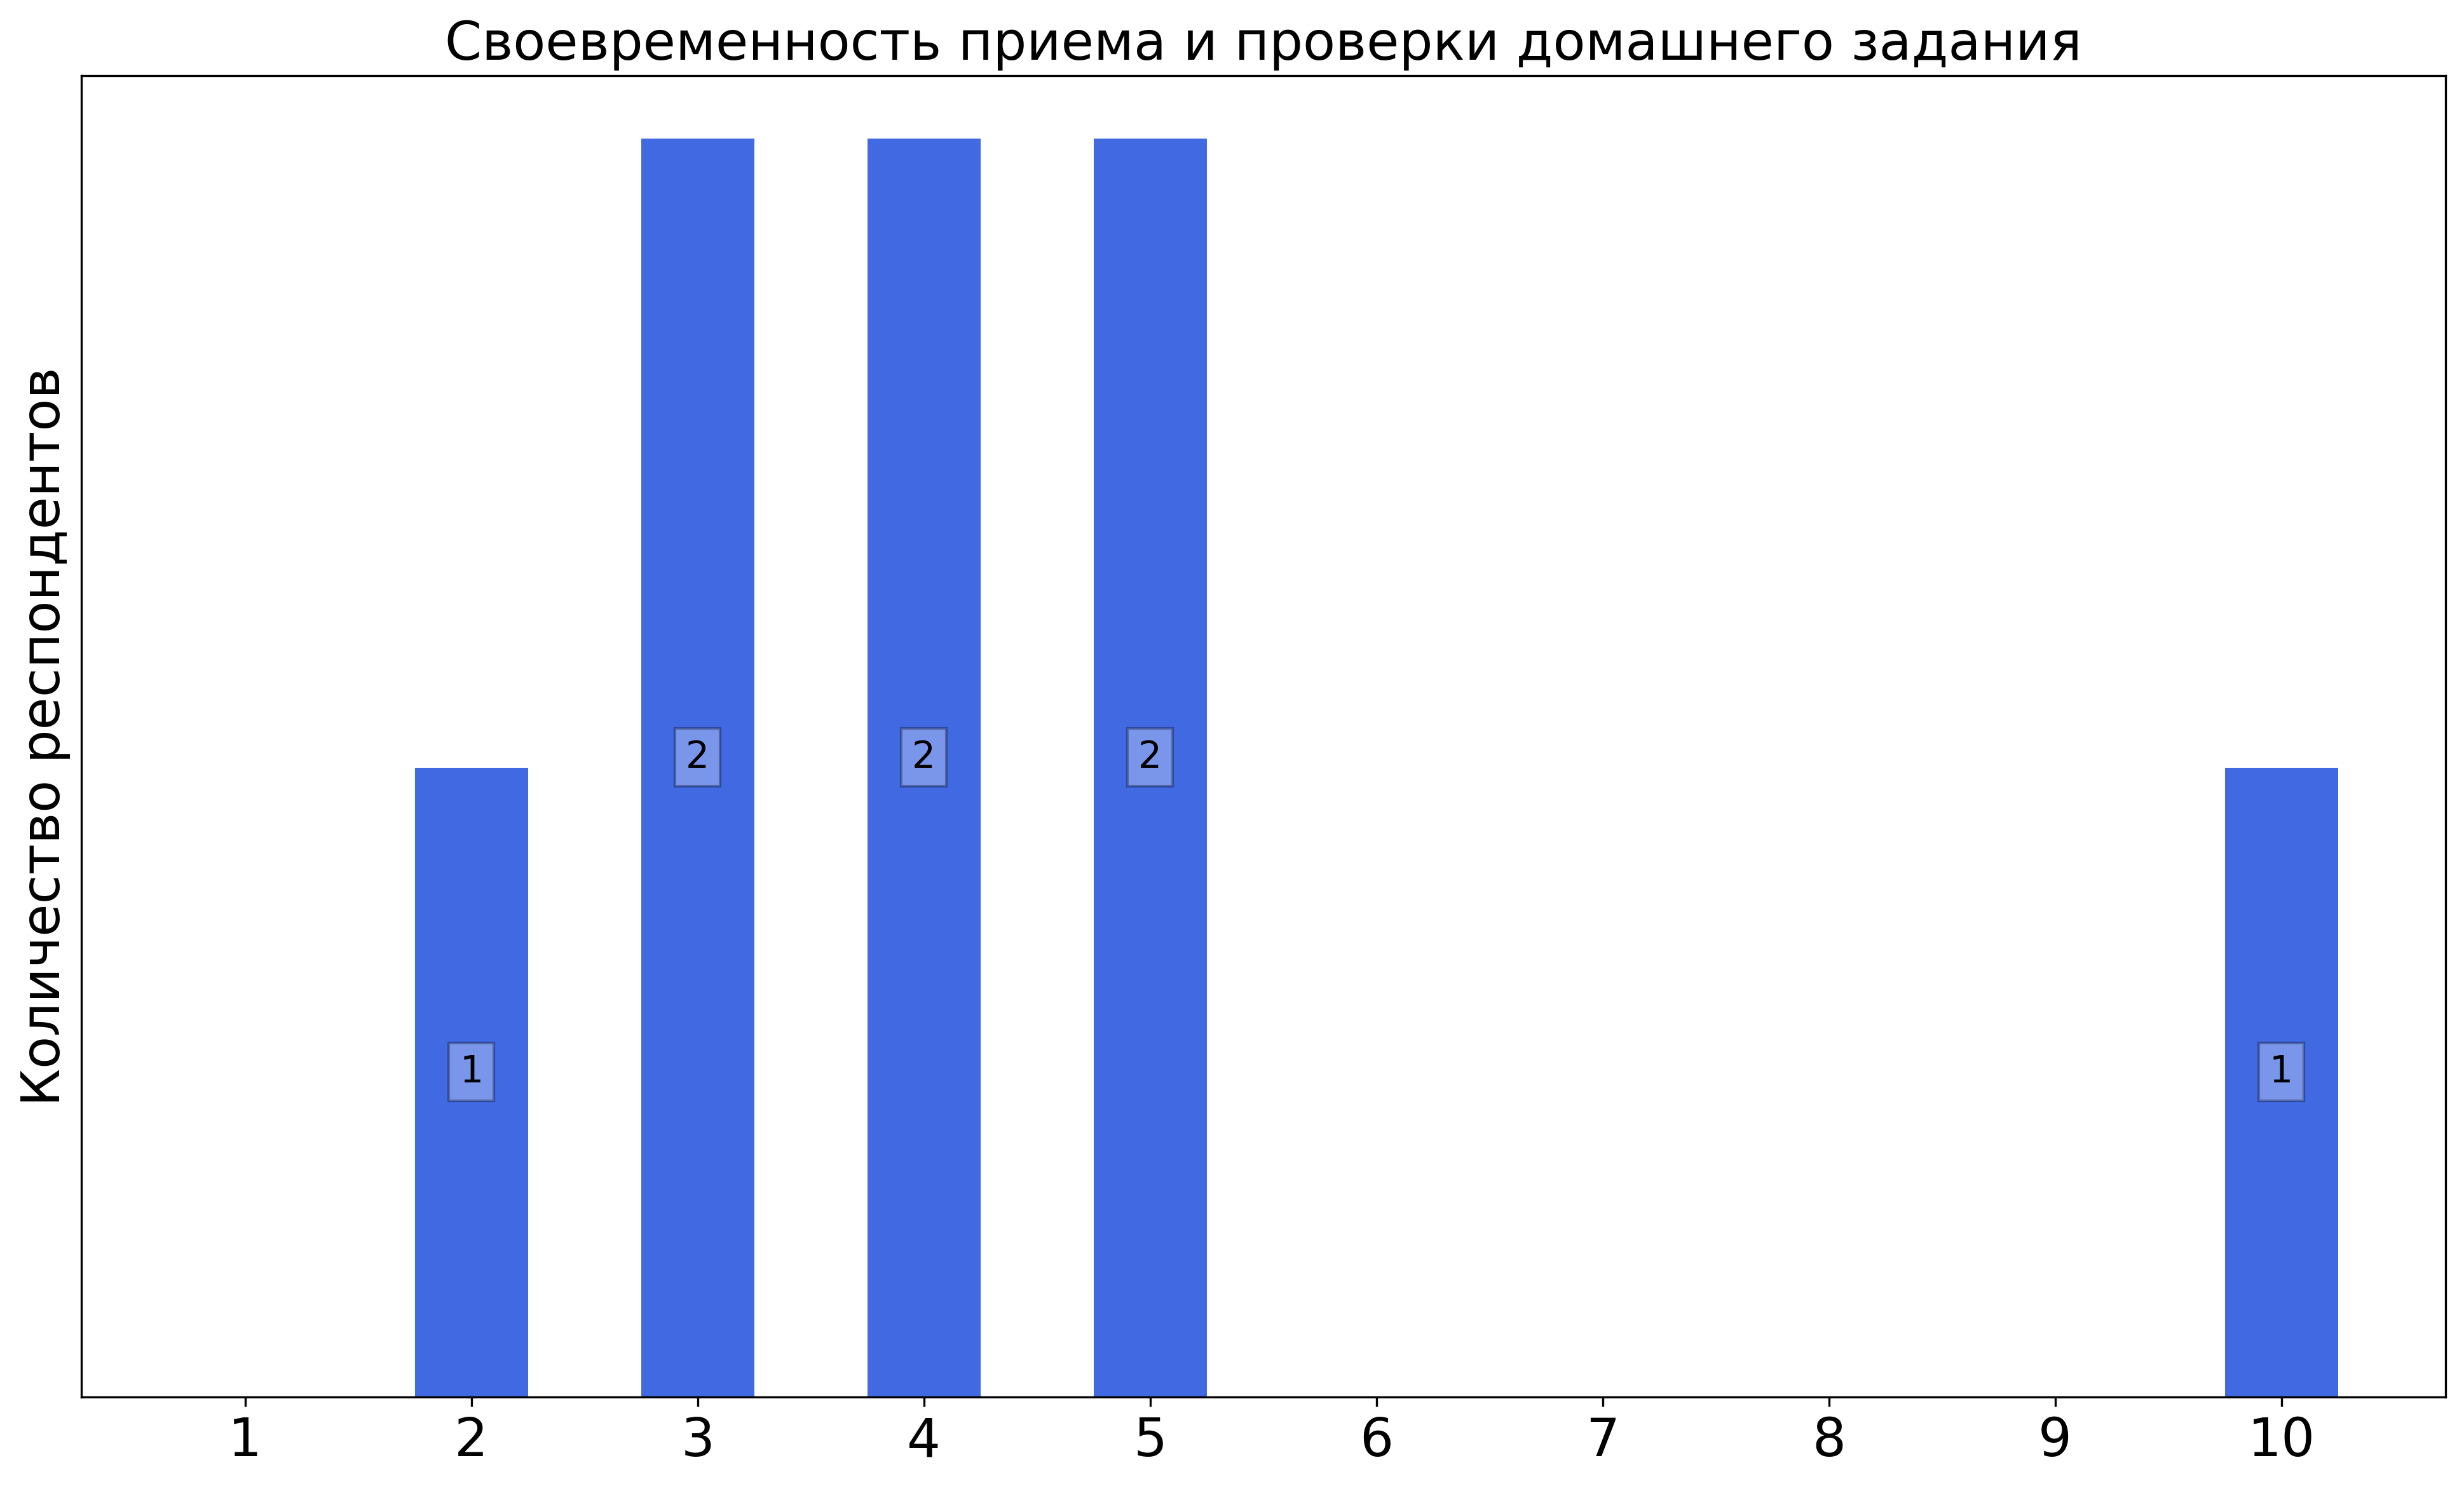
\includegraphics[width=\textwidth]{images/3 course/Теория поля/seminarists-marks-Девизорова Ж.А.-2.png}
            \end{subfigure}
            \begin{subfigure}[b]{0.45\textwidth}
                \centering
                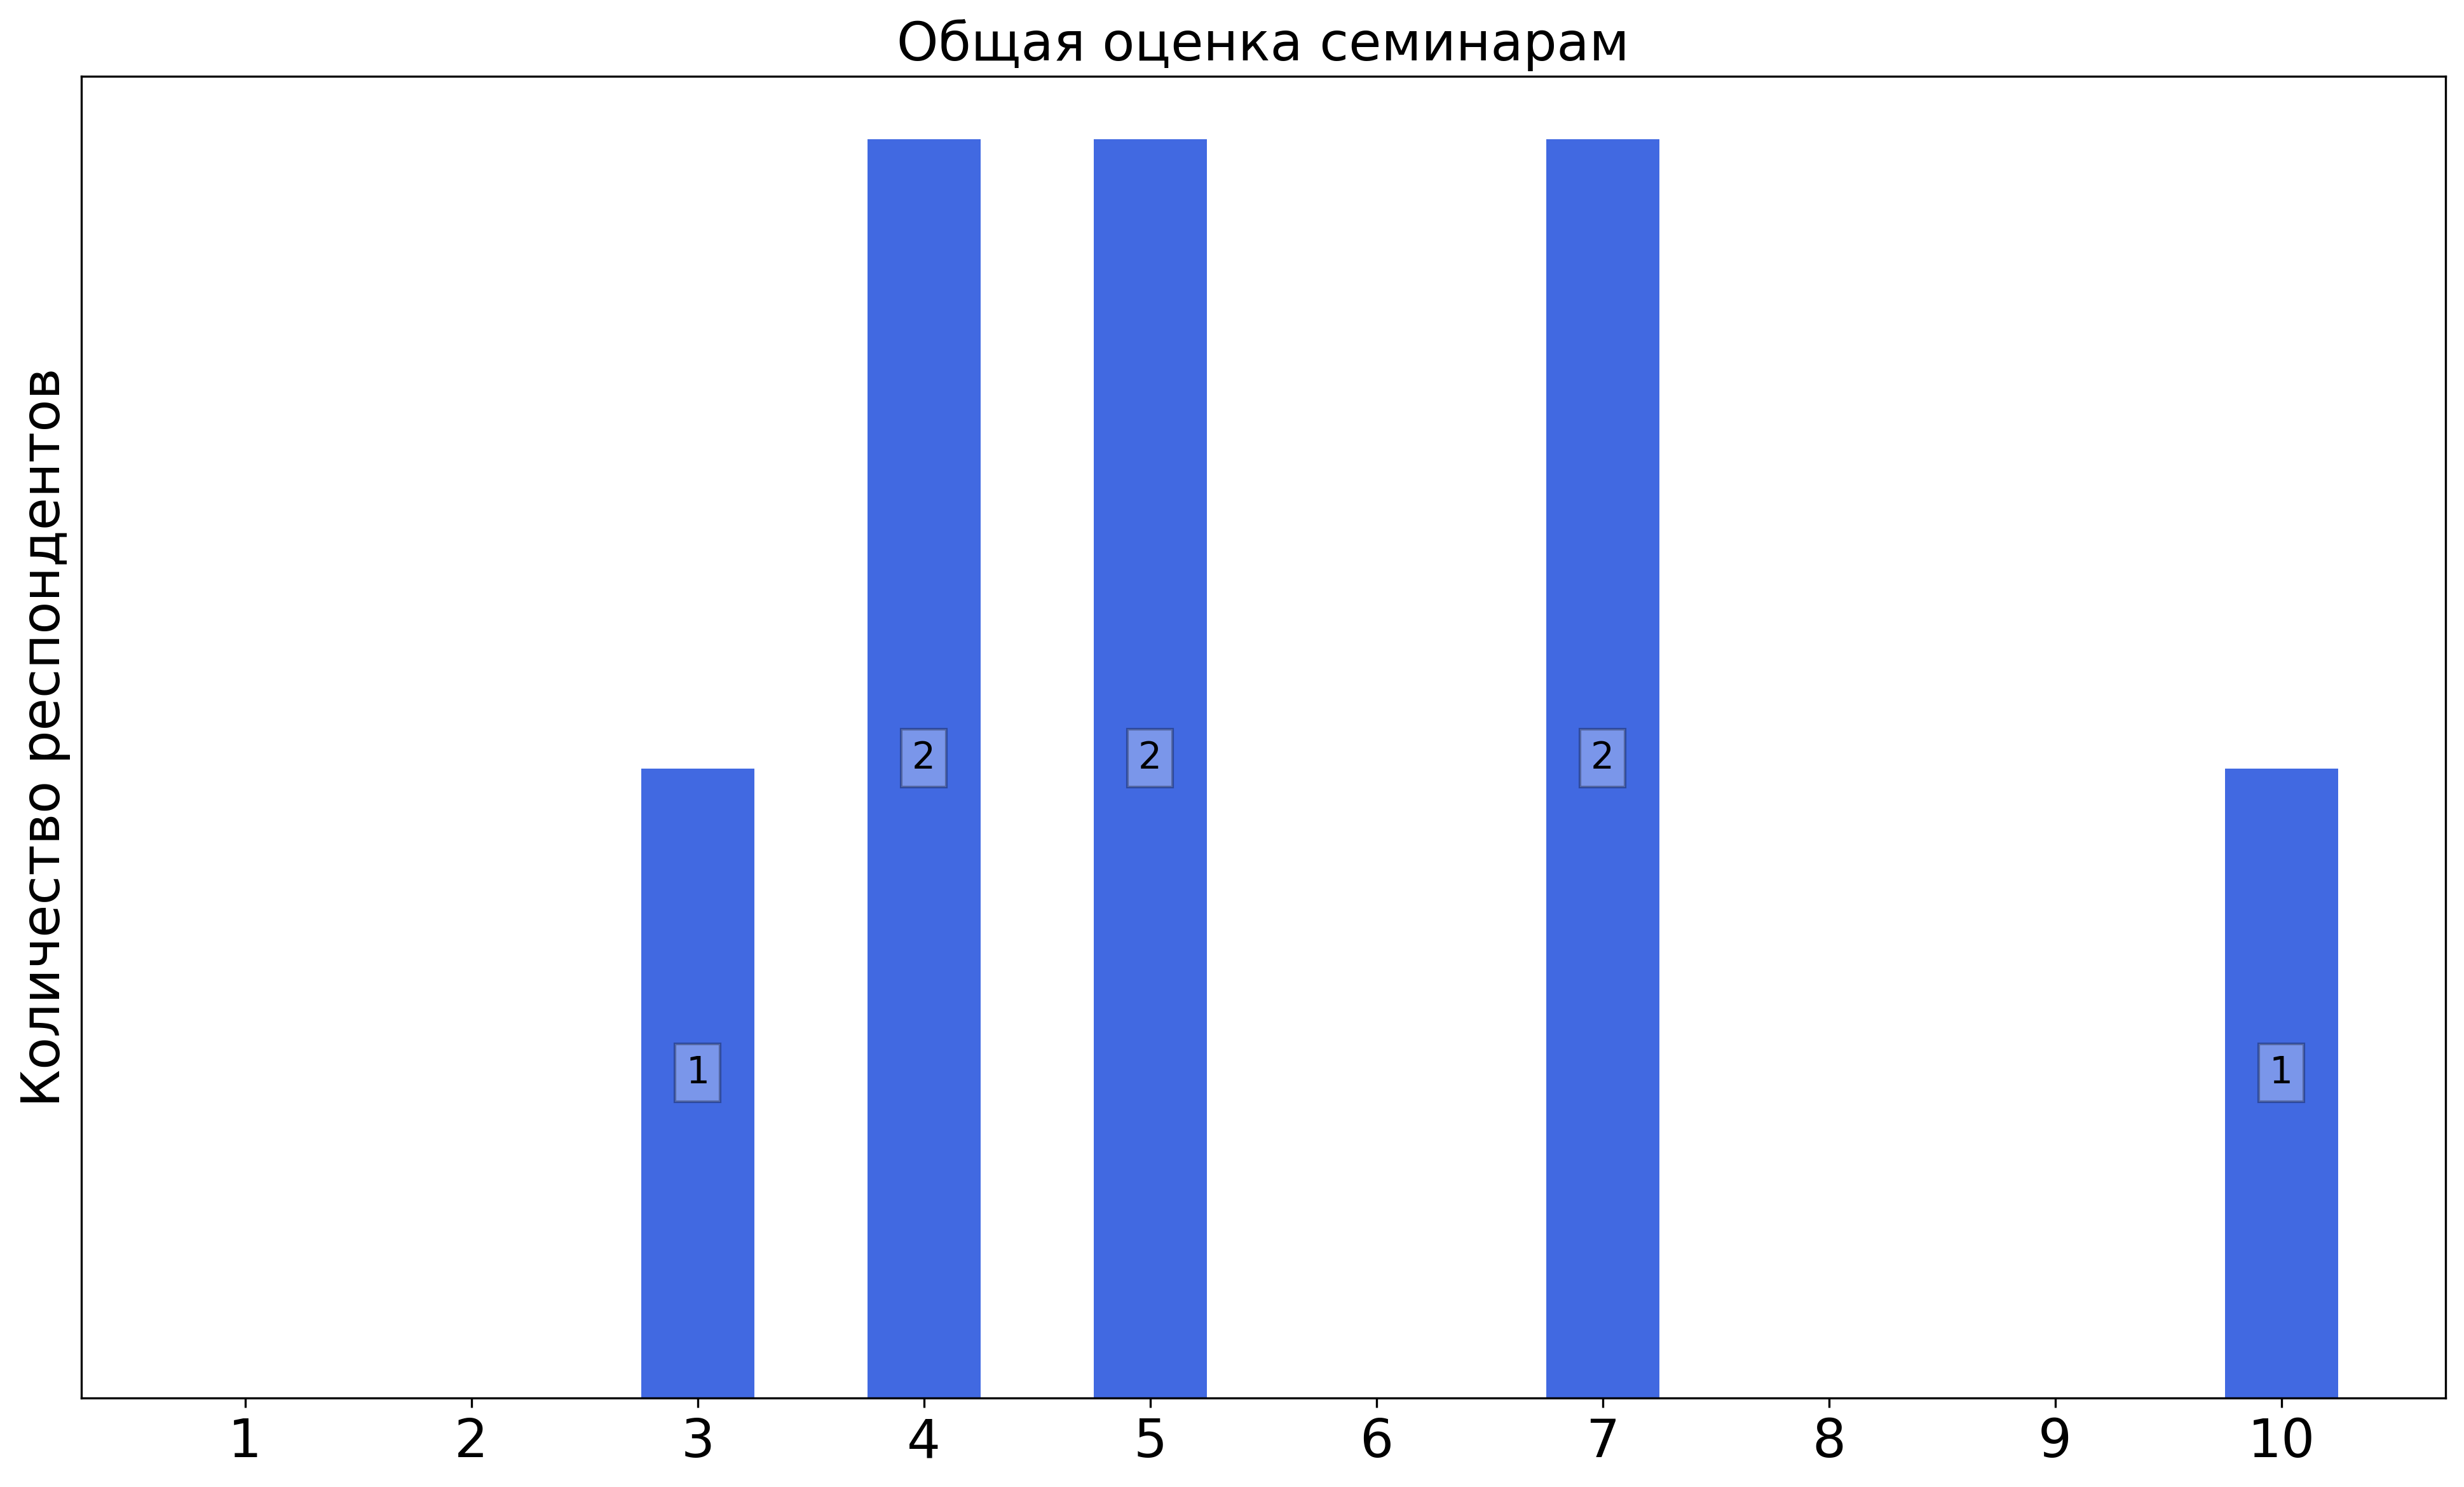
\includegraphics[width=\textwidth]{images/3 course/Теория поля/seminarists-marks-Девизорова Ж.А.-3.png}
            \end{subfigure}	
            \caption{Оценки респондентов о качестве преподавания семинаров}
        \end{figure}

        \textbf{Комментарии студентов о семинаристе\protect\footnote{сохранены оригинальные орфография и пунктуация}}
            \begin{commentbox} 
                Опаздывала на сдачи, один раз убежала на работу во время пар по расписанию (!), не готовидась к семинарам. Объясняет не очень понятно. И жестит с контрольными  
            \end{commentbox} 
        
            \begin{commentbox} 
                Жанна Алексеевна отлично расшаривает теорпол 
            \end{commentbox} 
        
            \begin{commentbox} 
                Жанна Алексеевна по началу показалась хорошим семинаристом. Но все испортилось при первой же сдаче. 
        
                Во-первых, она затянулась на месяц, из-за полностью неадекватной системы сдачи. Нужно сидеть в очереди порядка 1.5 часов, чтобы в итоге поговорить от силы 5 минут, получить доп. вопрос, и сидеть еще столько же.
                
                Во-вторых, частые опоздания на установленные сдачи и семинары (или их пропуск) по абсолютно разным причинам. Приведу один пример... По расписанию была пара, на которой договорились устроить сдачу, группа пришла, но Жанна Алексеевна - нет, причиной тому была, цитирую: "Меня выдернули ПО ОСНОВНОЙ РАБОТЕ" (пара была по официальному расписанию МФТИ).
                
                В-третьих, полностью неадекватные контрольные и система оценивания. По итогу семестра, максимальный средний балл по двум группам был около 6.5, но Жанна Алексеевна решила раздать "ПОДАРКИ ОТ ДЕДА МОРОЗА". Кто ей понравился - добавила 1-2 балла к итоговой. Зачем было весь семестр напрягаться, делать д/з, что-то зашаривать, если все решило ее субъективное мнение? 
                
                Оценка не важны, важны знания, скажите вы, и будете полностью правы, но какая мотивация изучать предмет, когда тебе недостойно оценивают? 
            \end{commentbox} 
        
            \begin{commentbox} 
                сдачи очень долгие( 
            \end{commentbox} 
        
            \begin{commentbox} 
                Не желаю к ней попасться. Объясняет материал плохо, оперирует непонятными никому вещами, говорит больше про математику, чем про физику. Иногда у нее какие-то задержки в обработке вопроса, что выглядит странным, когда в итоге отвечает на вопрос, то вопросов становится еще больше. Сдача дз - кошмар. Она конечно согласует с вами какое-то удобное(ей) время, но не факт что она придет к этому времени на сдачу)))), потому что ее могут вызвать по работе, ей поздно ехать, или она заболела. А когда все-таки сдача происходит, то длится что 3-5 часов. Причем ты просто ждешь когда она до тебя дойдет. А когда до тебя дойдет, то будет задавать понятные только ей вопросы по задаче, и если ты на них не ответишь, то она тебя оставит с ними подумать и уйдет к другим, а ты будешь ждать своей очереди еще час). Из-за ее схемы проверки дз, получить высокий балл тяжело, надо решать задачи, а делать это не хочется из-за уже потраченного времени, либо задачи хардовые, а терпел с ней ботать нереально. Кр ее это еще хуже история. Задачи сложнее чем в задании, а так как задачи она решать вас не научит, то и баллы будут соответствующие, так что почти у всей группы рек к экзу был 4,5,6. Вот такие пироги. 
            \end{commentbox} 


    \subsubsection{Отзыв студентов о семинарах. Семинарист: Дудченко В.А.}
        \begin{figure}[H]
            \centering
            \begin{subfigure}[b]{0.45\textwidth}
                \centering
                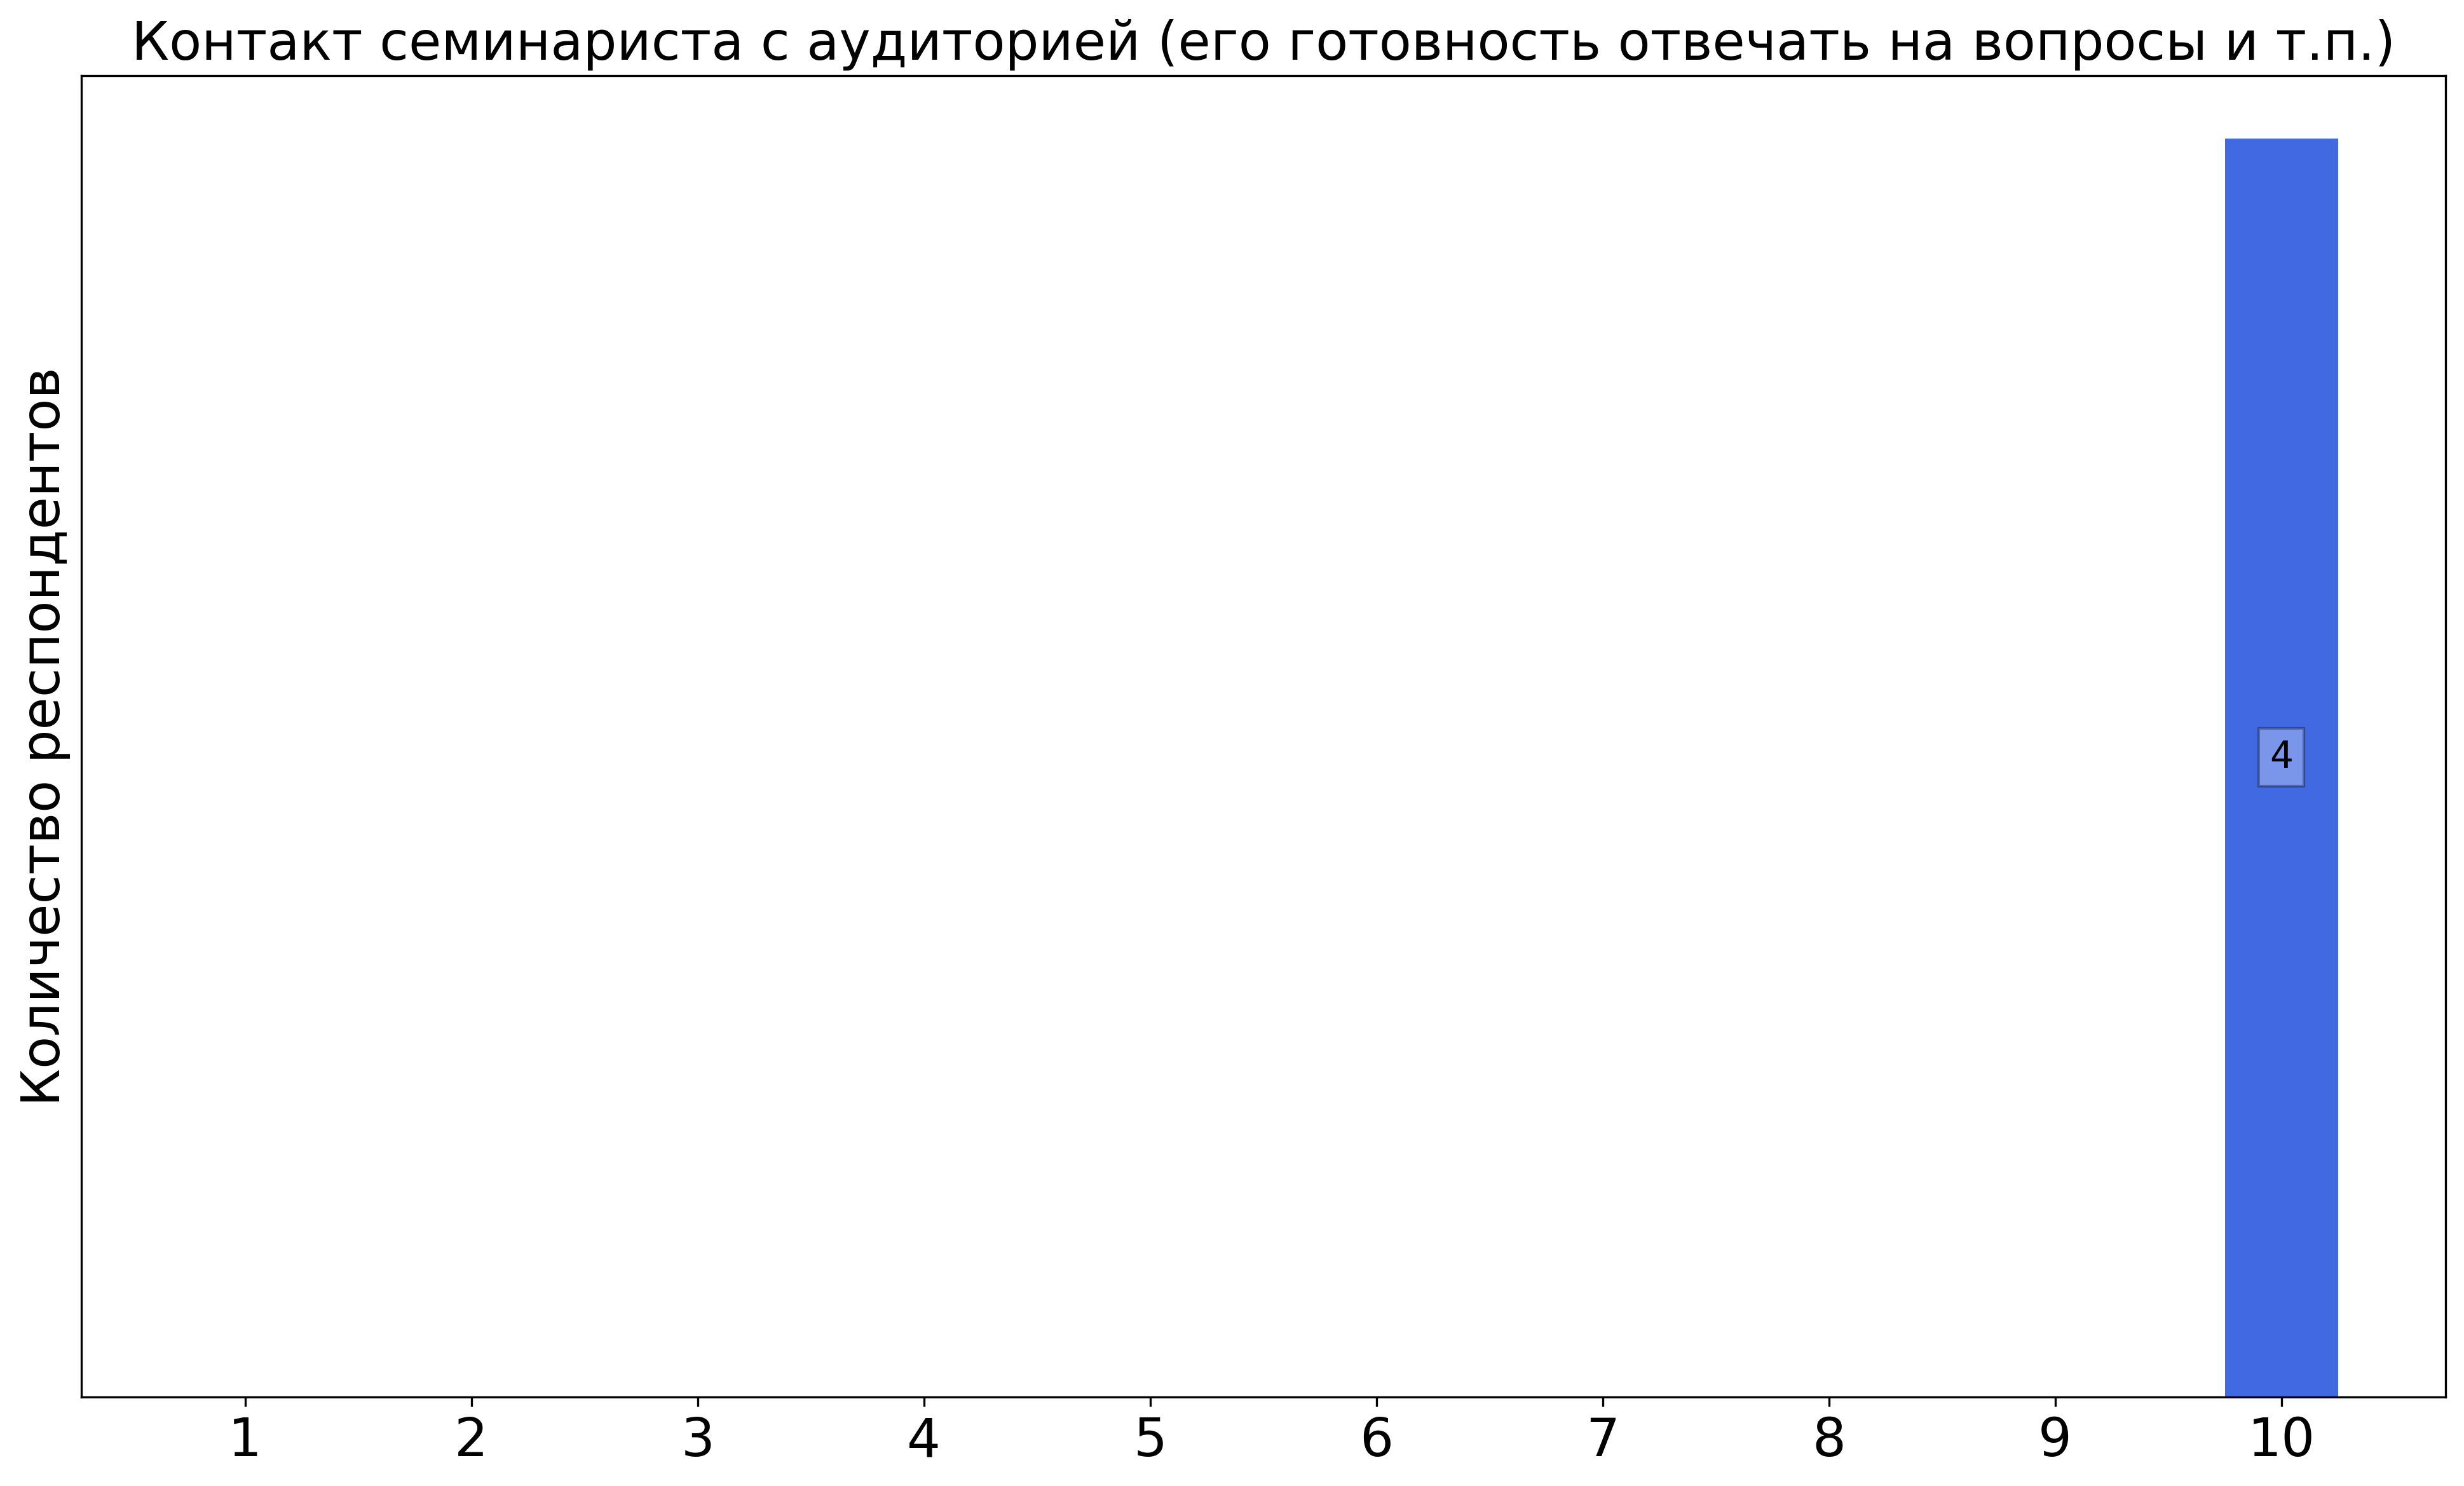
\includegraphics[width=\textwidth]{images/3 course/Теория поля/seminarists-marks-Дудченко В.А.-0.png}
            \end{subfigure}
            \begin{subfigure}[b]{0.45\textwidth}
                \centering
                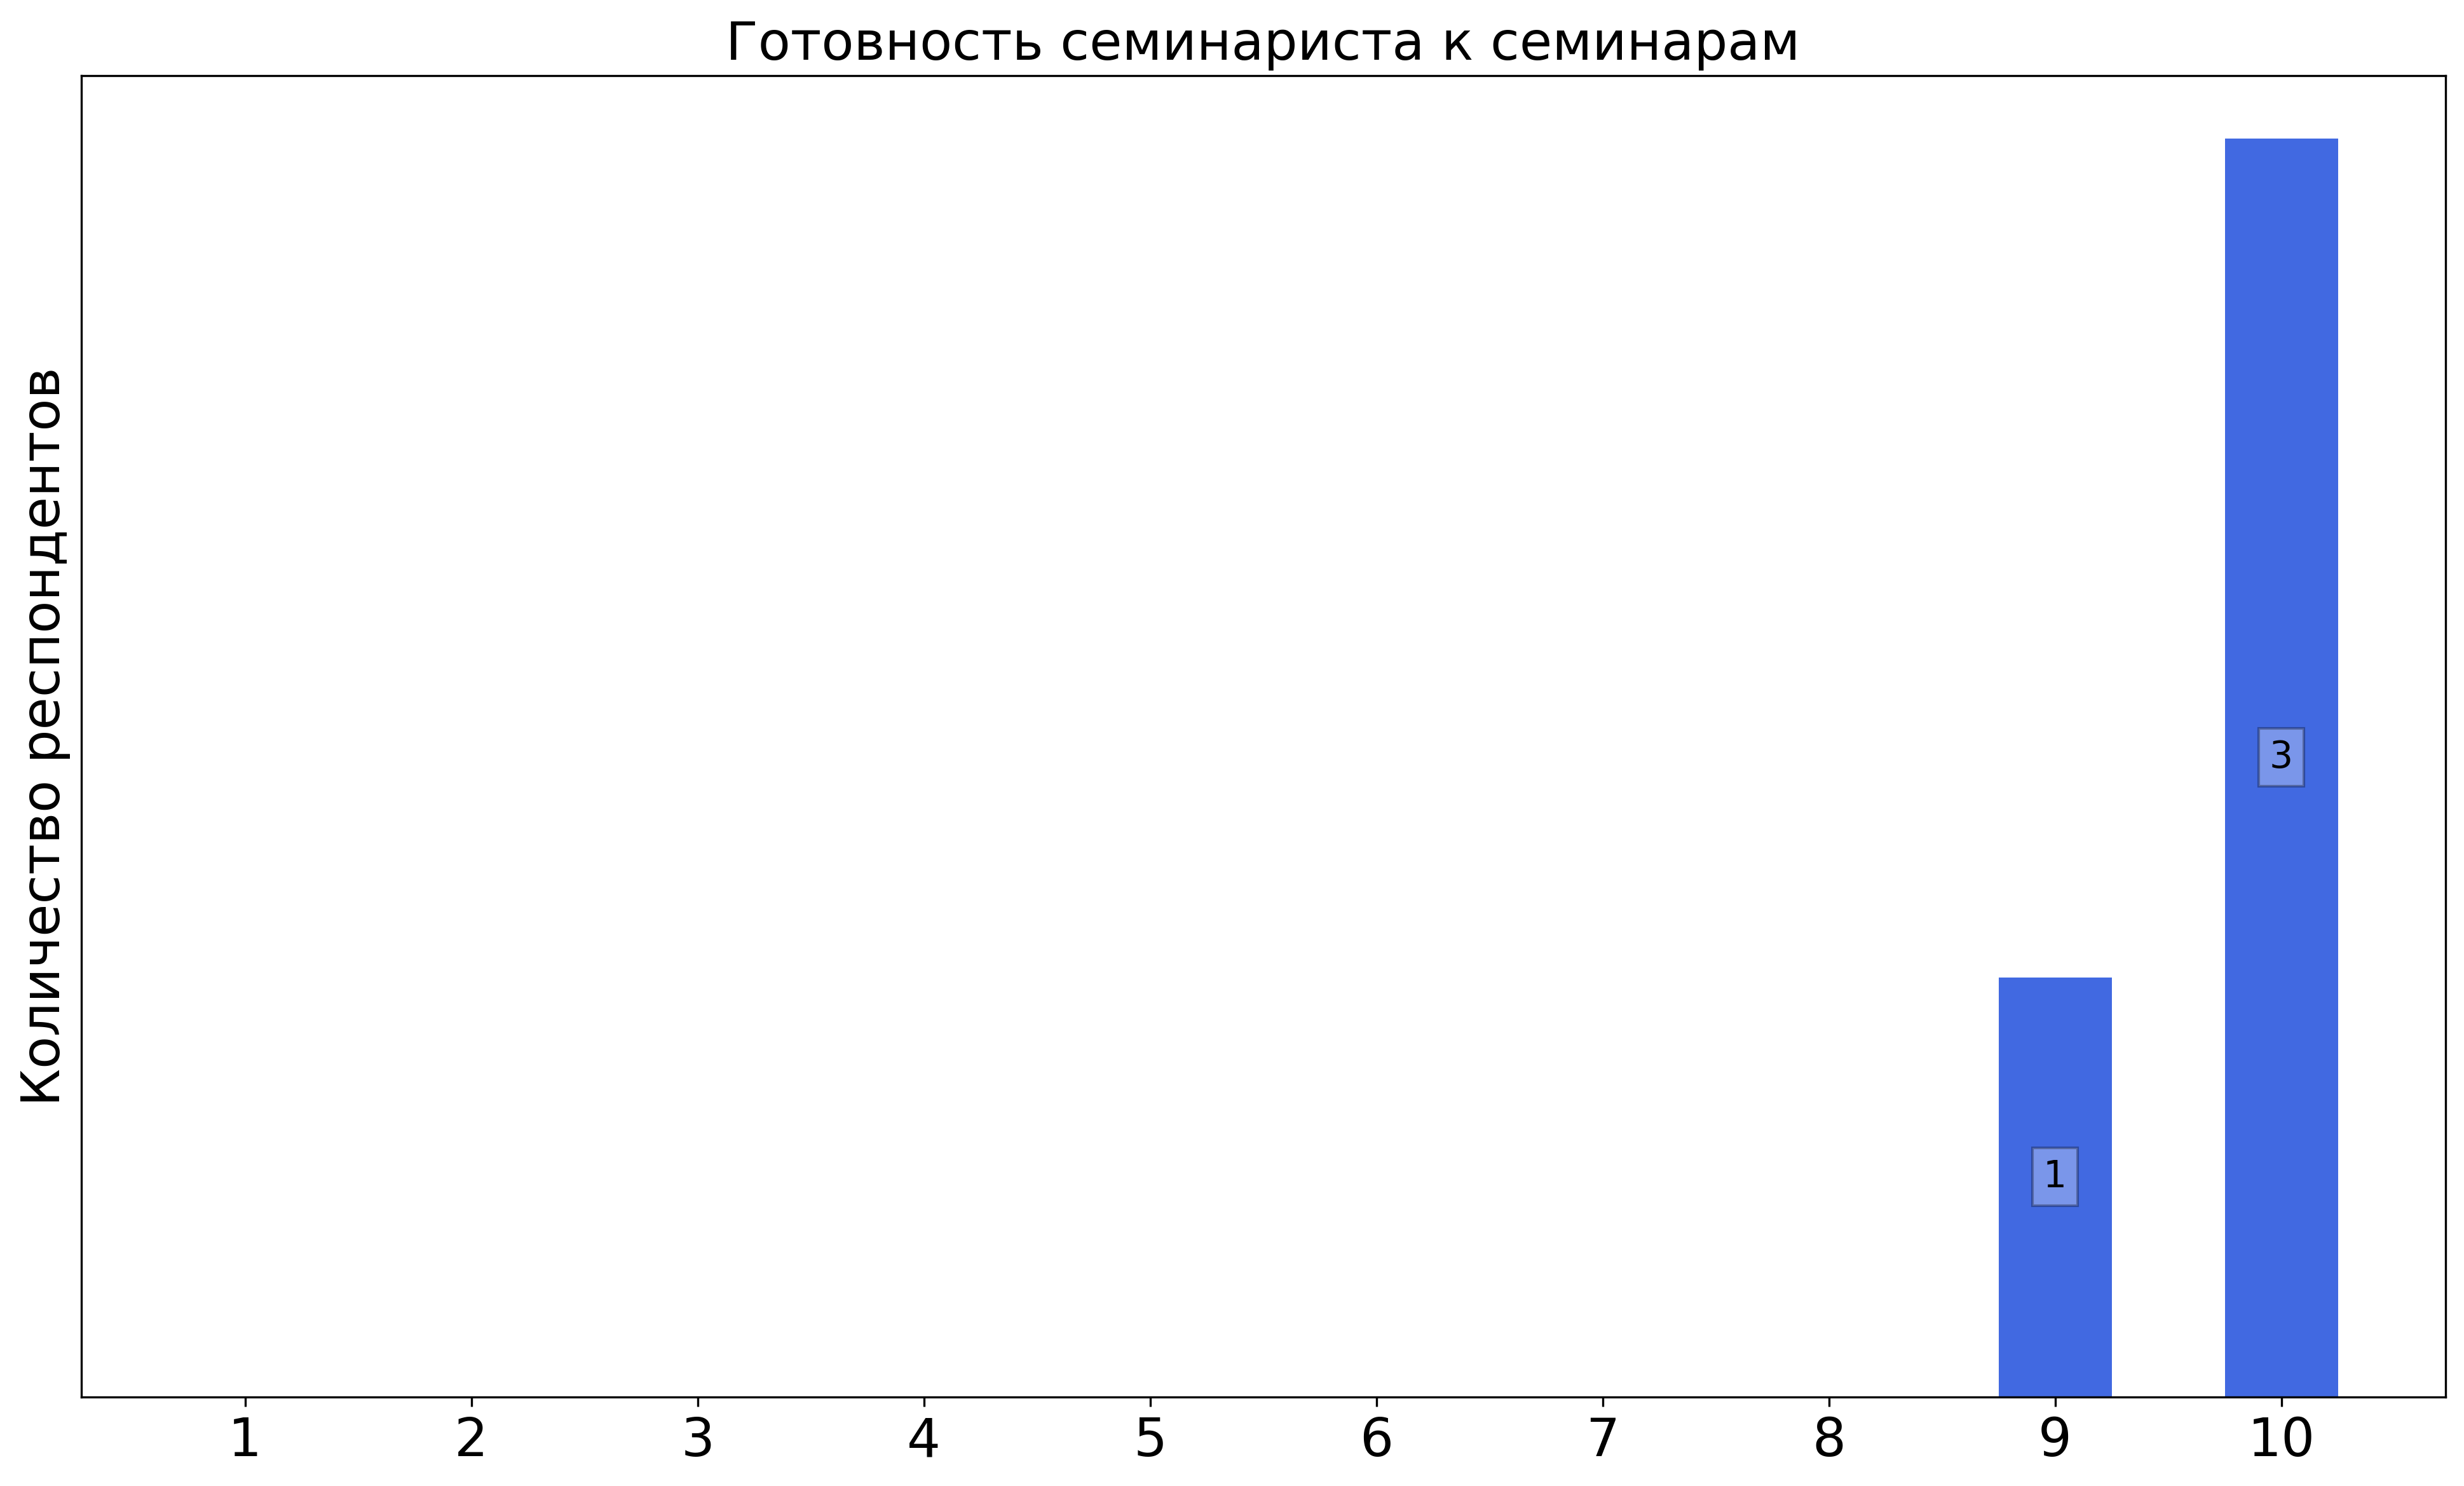
\includegraphics[width=\textwidth]{images/3 course/Теория поля/seminarists-marks-Дудченко В.А.-1.png}
            \end{subfigure}
            \begin{subfigure}[b]{0.45\textwidth}
                \centering
                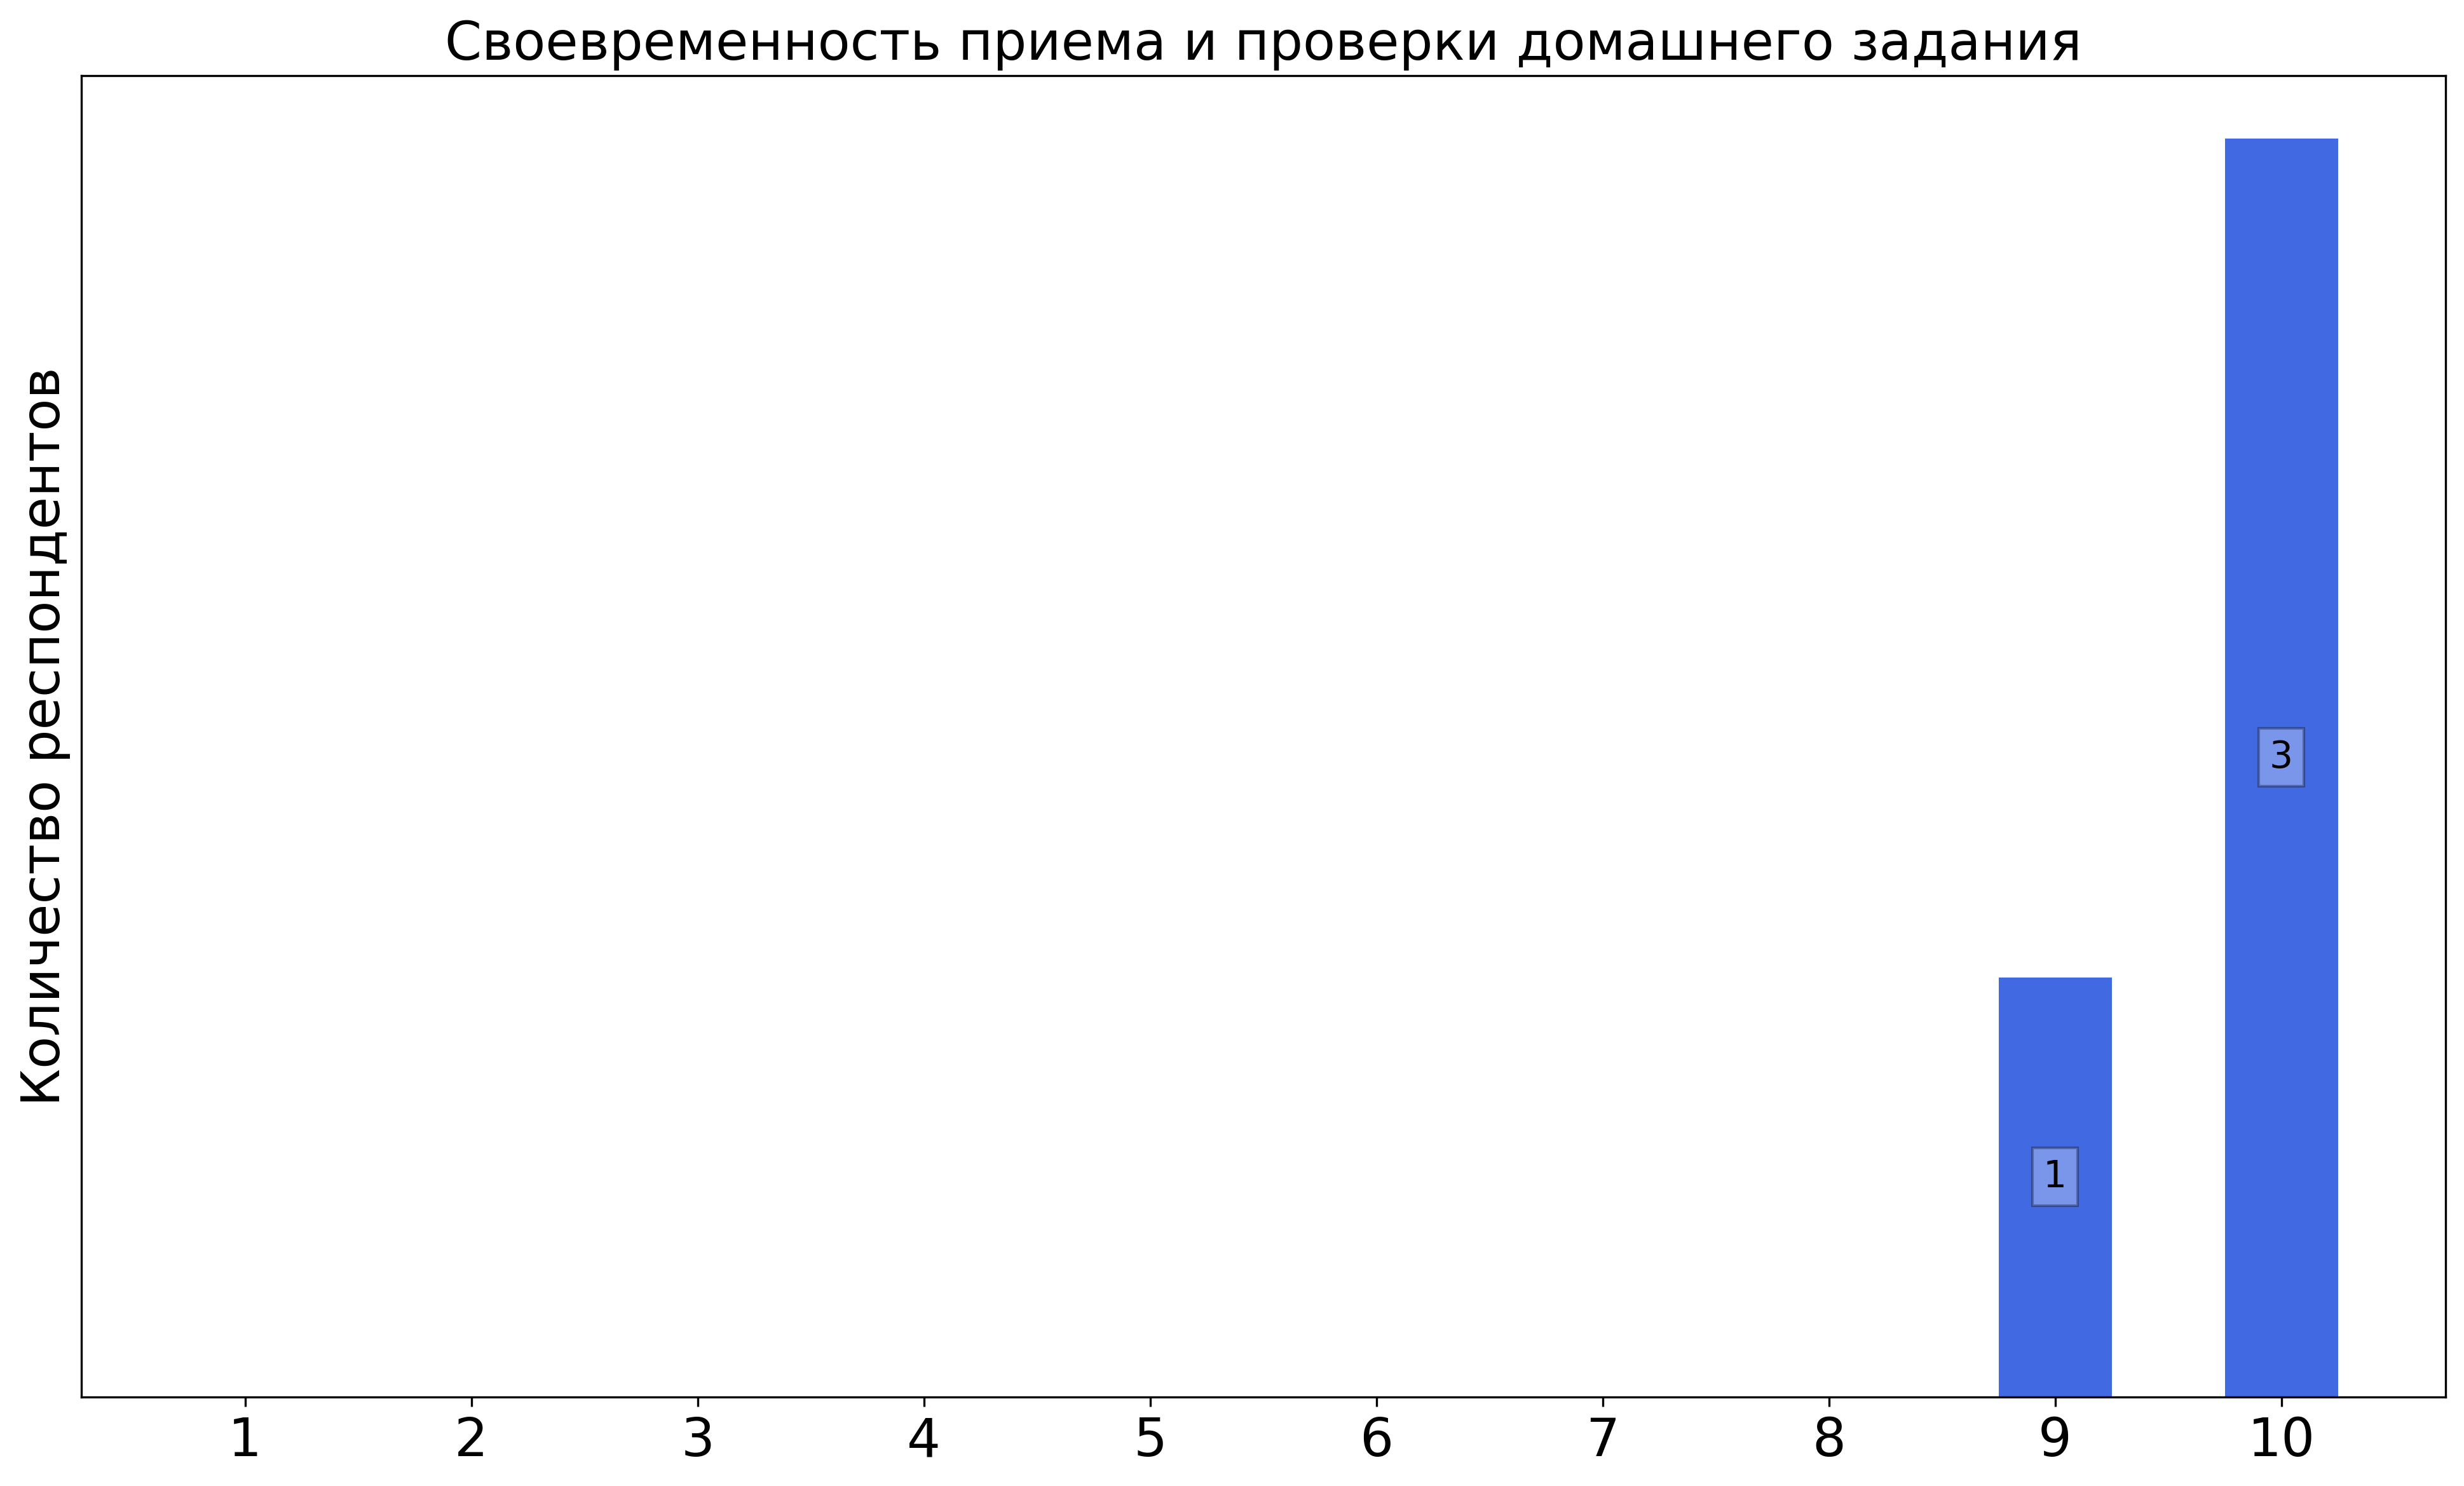
\includegraphics[width=\textwidth]{images/3 course/Теория поля/seminarists-marks-Дудченко В.А.-2.png}
            \end{subfigure}
            \begin{subfigure}[b]{0.45\textwidth}
                \centering
                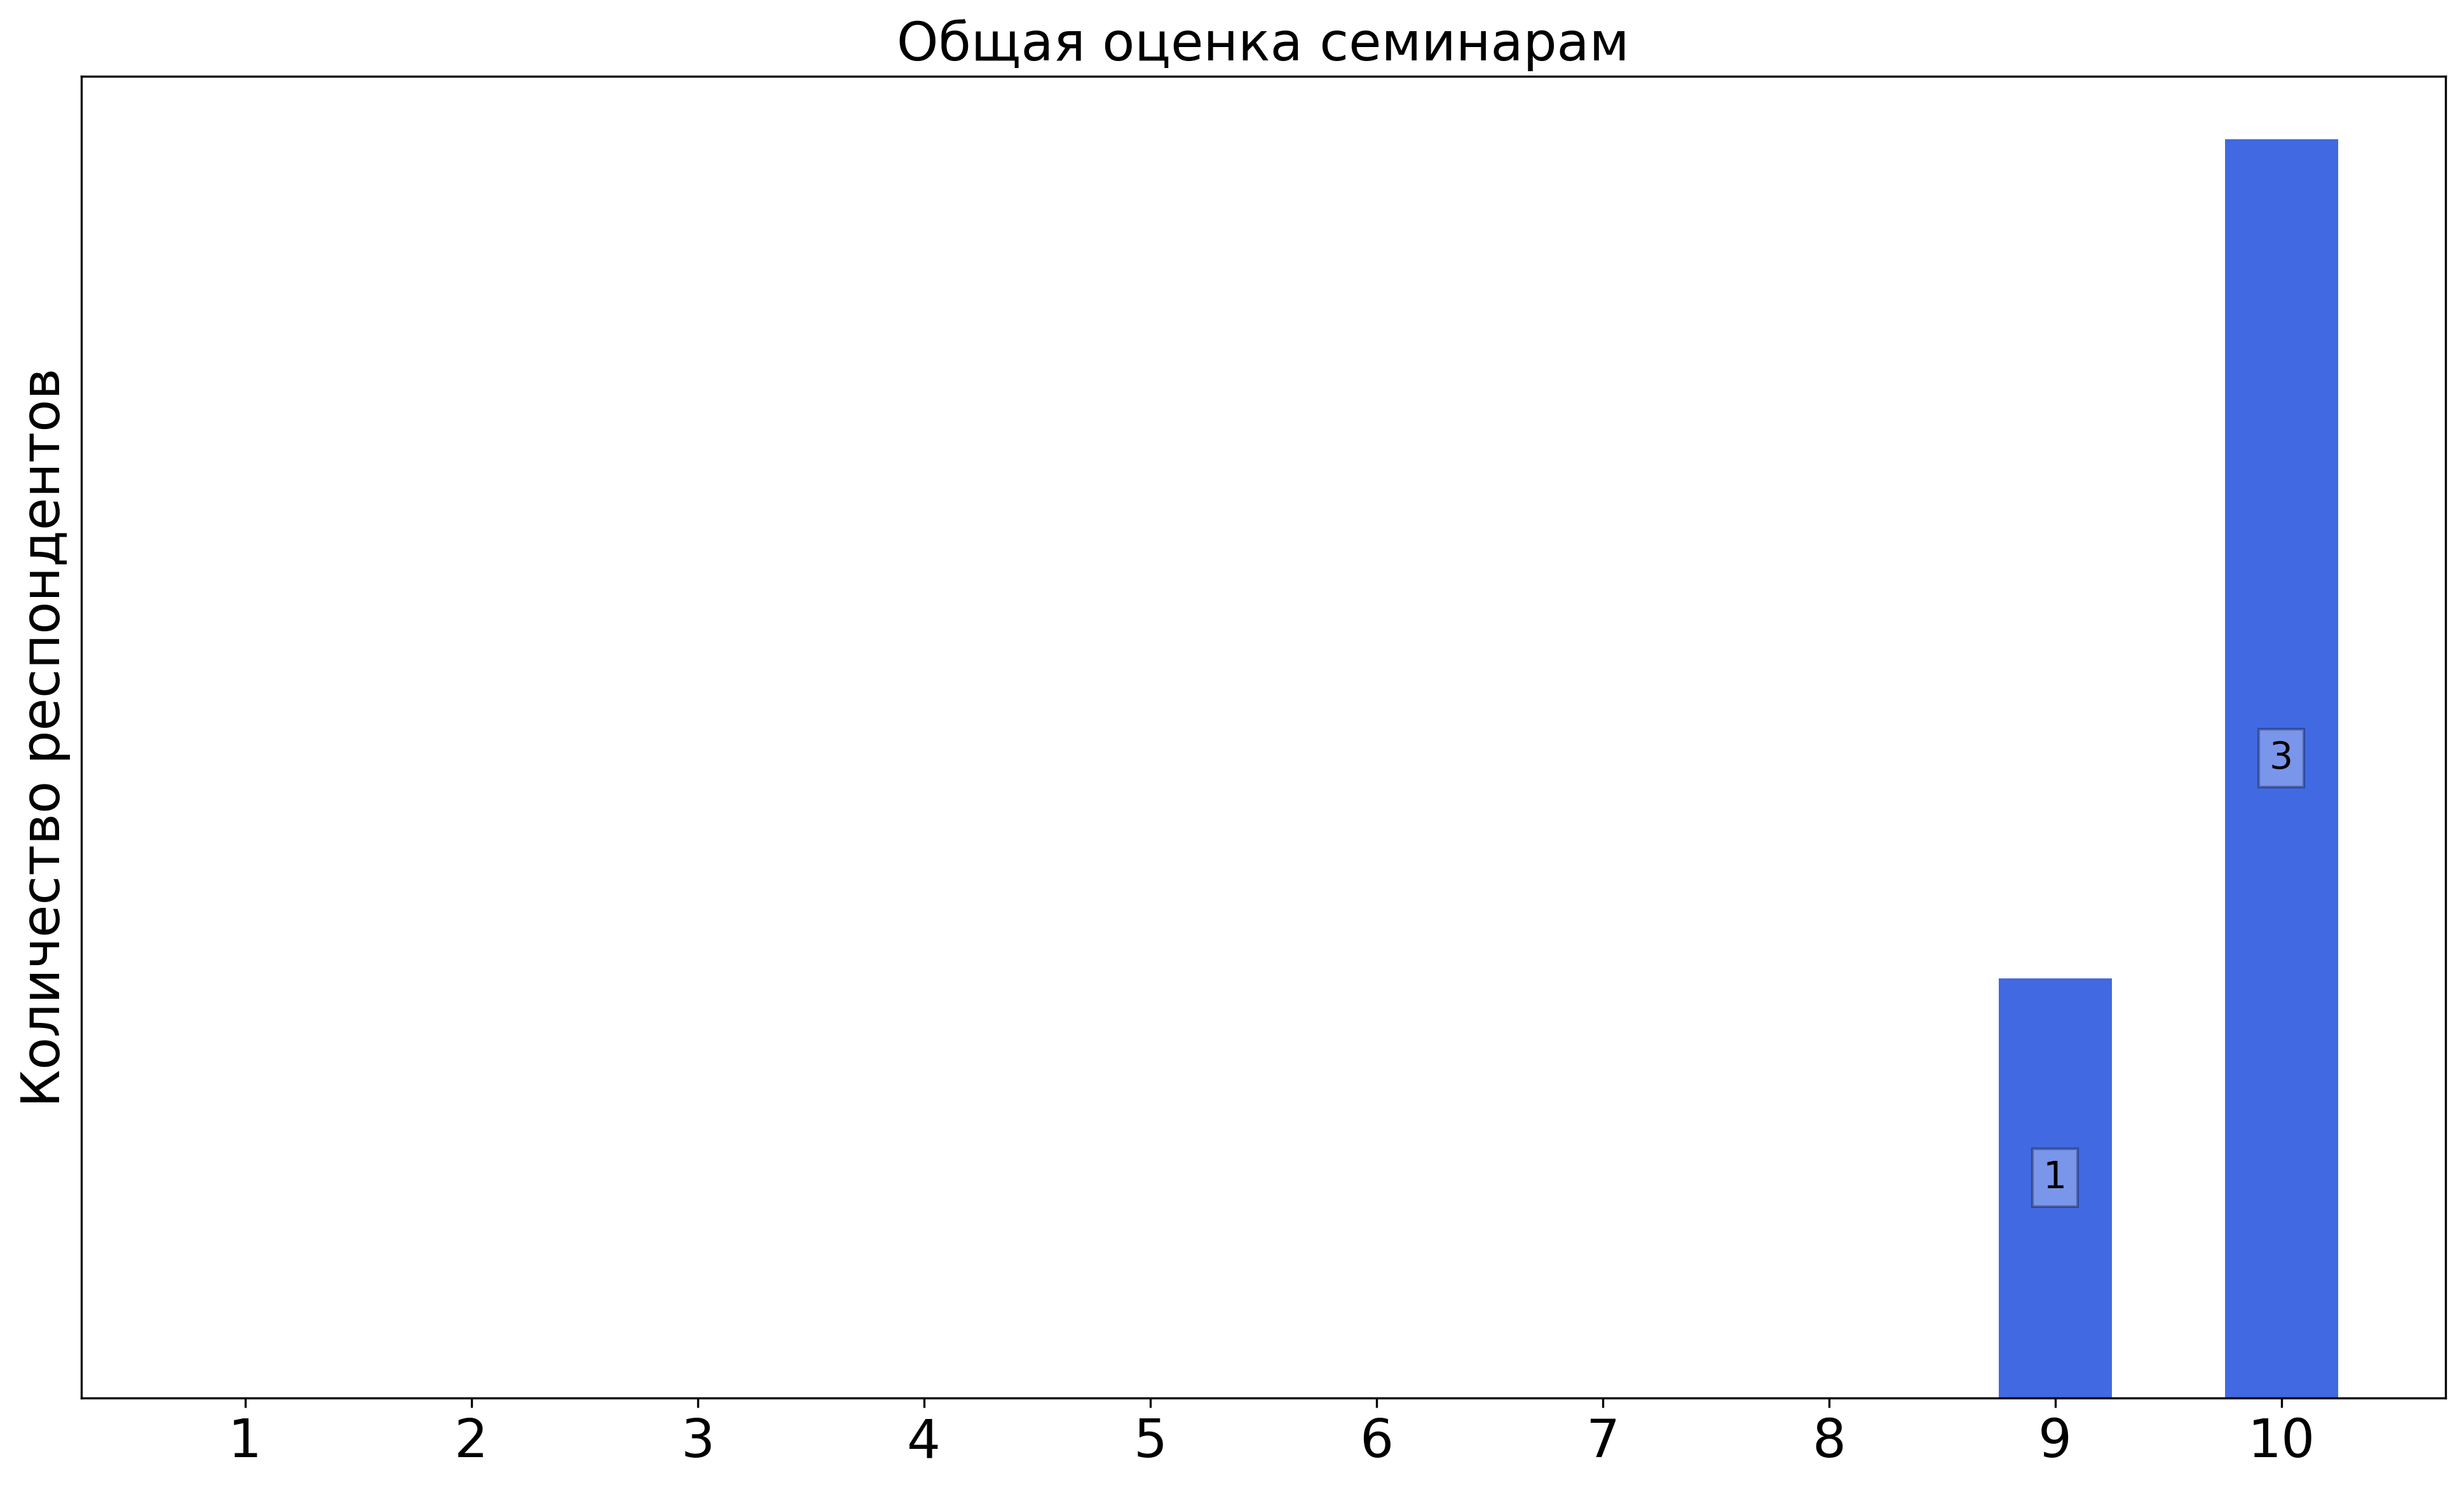
\includegraphics[width=\textwidth]{images/3 course/Теория поля/seminarists-marks-Дудченко В.А.-3.png}
            \end{subfigure}	
            \caption{Оценки респондентов о качестве преподавания семинаров}
        \end{figure}

        \textbf{Комментарии студентов о семинаристе\protect\footnote{сохранены оригинальные орфография и пунктуация}}
            \begin{commentbox} 
                Прекрасный семинарист. В ходе семинаров разбираются задачи из дз, при этом решение задач проходит "в режиме реального времени", когда нас наталкивают на мысль, а мы должны сделать какое-то промежуточное вычисление и осознать суть задачи. Объяснения чёткие и понятные, темп отличный, критерии оценивания тоже адекватные  
            \end{commentbox} 
        
            \begin{commentbox} 
                В начале было тяжело, преподаватель ведет первый год. Но к середине семестра семинары стали понятными, помогали восприятию курса.  
            \end{commentbox} 
        
            \begin{commentbox} 
                Семинары проходят очень приятно. Преподаватель всегда отвечает на все вопросы. Разбираются задачи понятно  
            \end{commentbox} 
        
            \begin{commentbox} 
                Семинарист отличный, если бы не он впечатление о курсе явно было бы сильно хуже. Преподаёт живо и с интересом, всегда готов ответить на вопросы, оценивает адекватно. 
            \end{commentbox} 


    \subsubsection{Отзыв студентов о семинарах. Семинарист: Дьяконов Д.В.}
        \begin{figure}[H]
            \centering
            \begin{subfigure}[b]{0.45\textwidth}
                \centering
                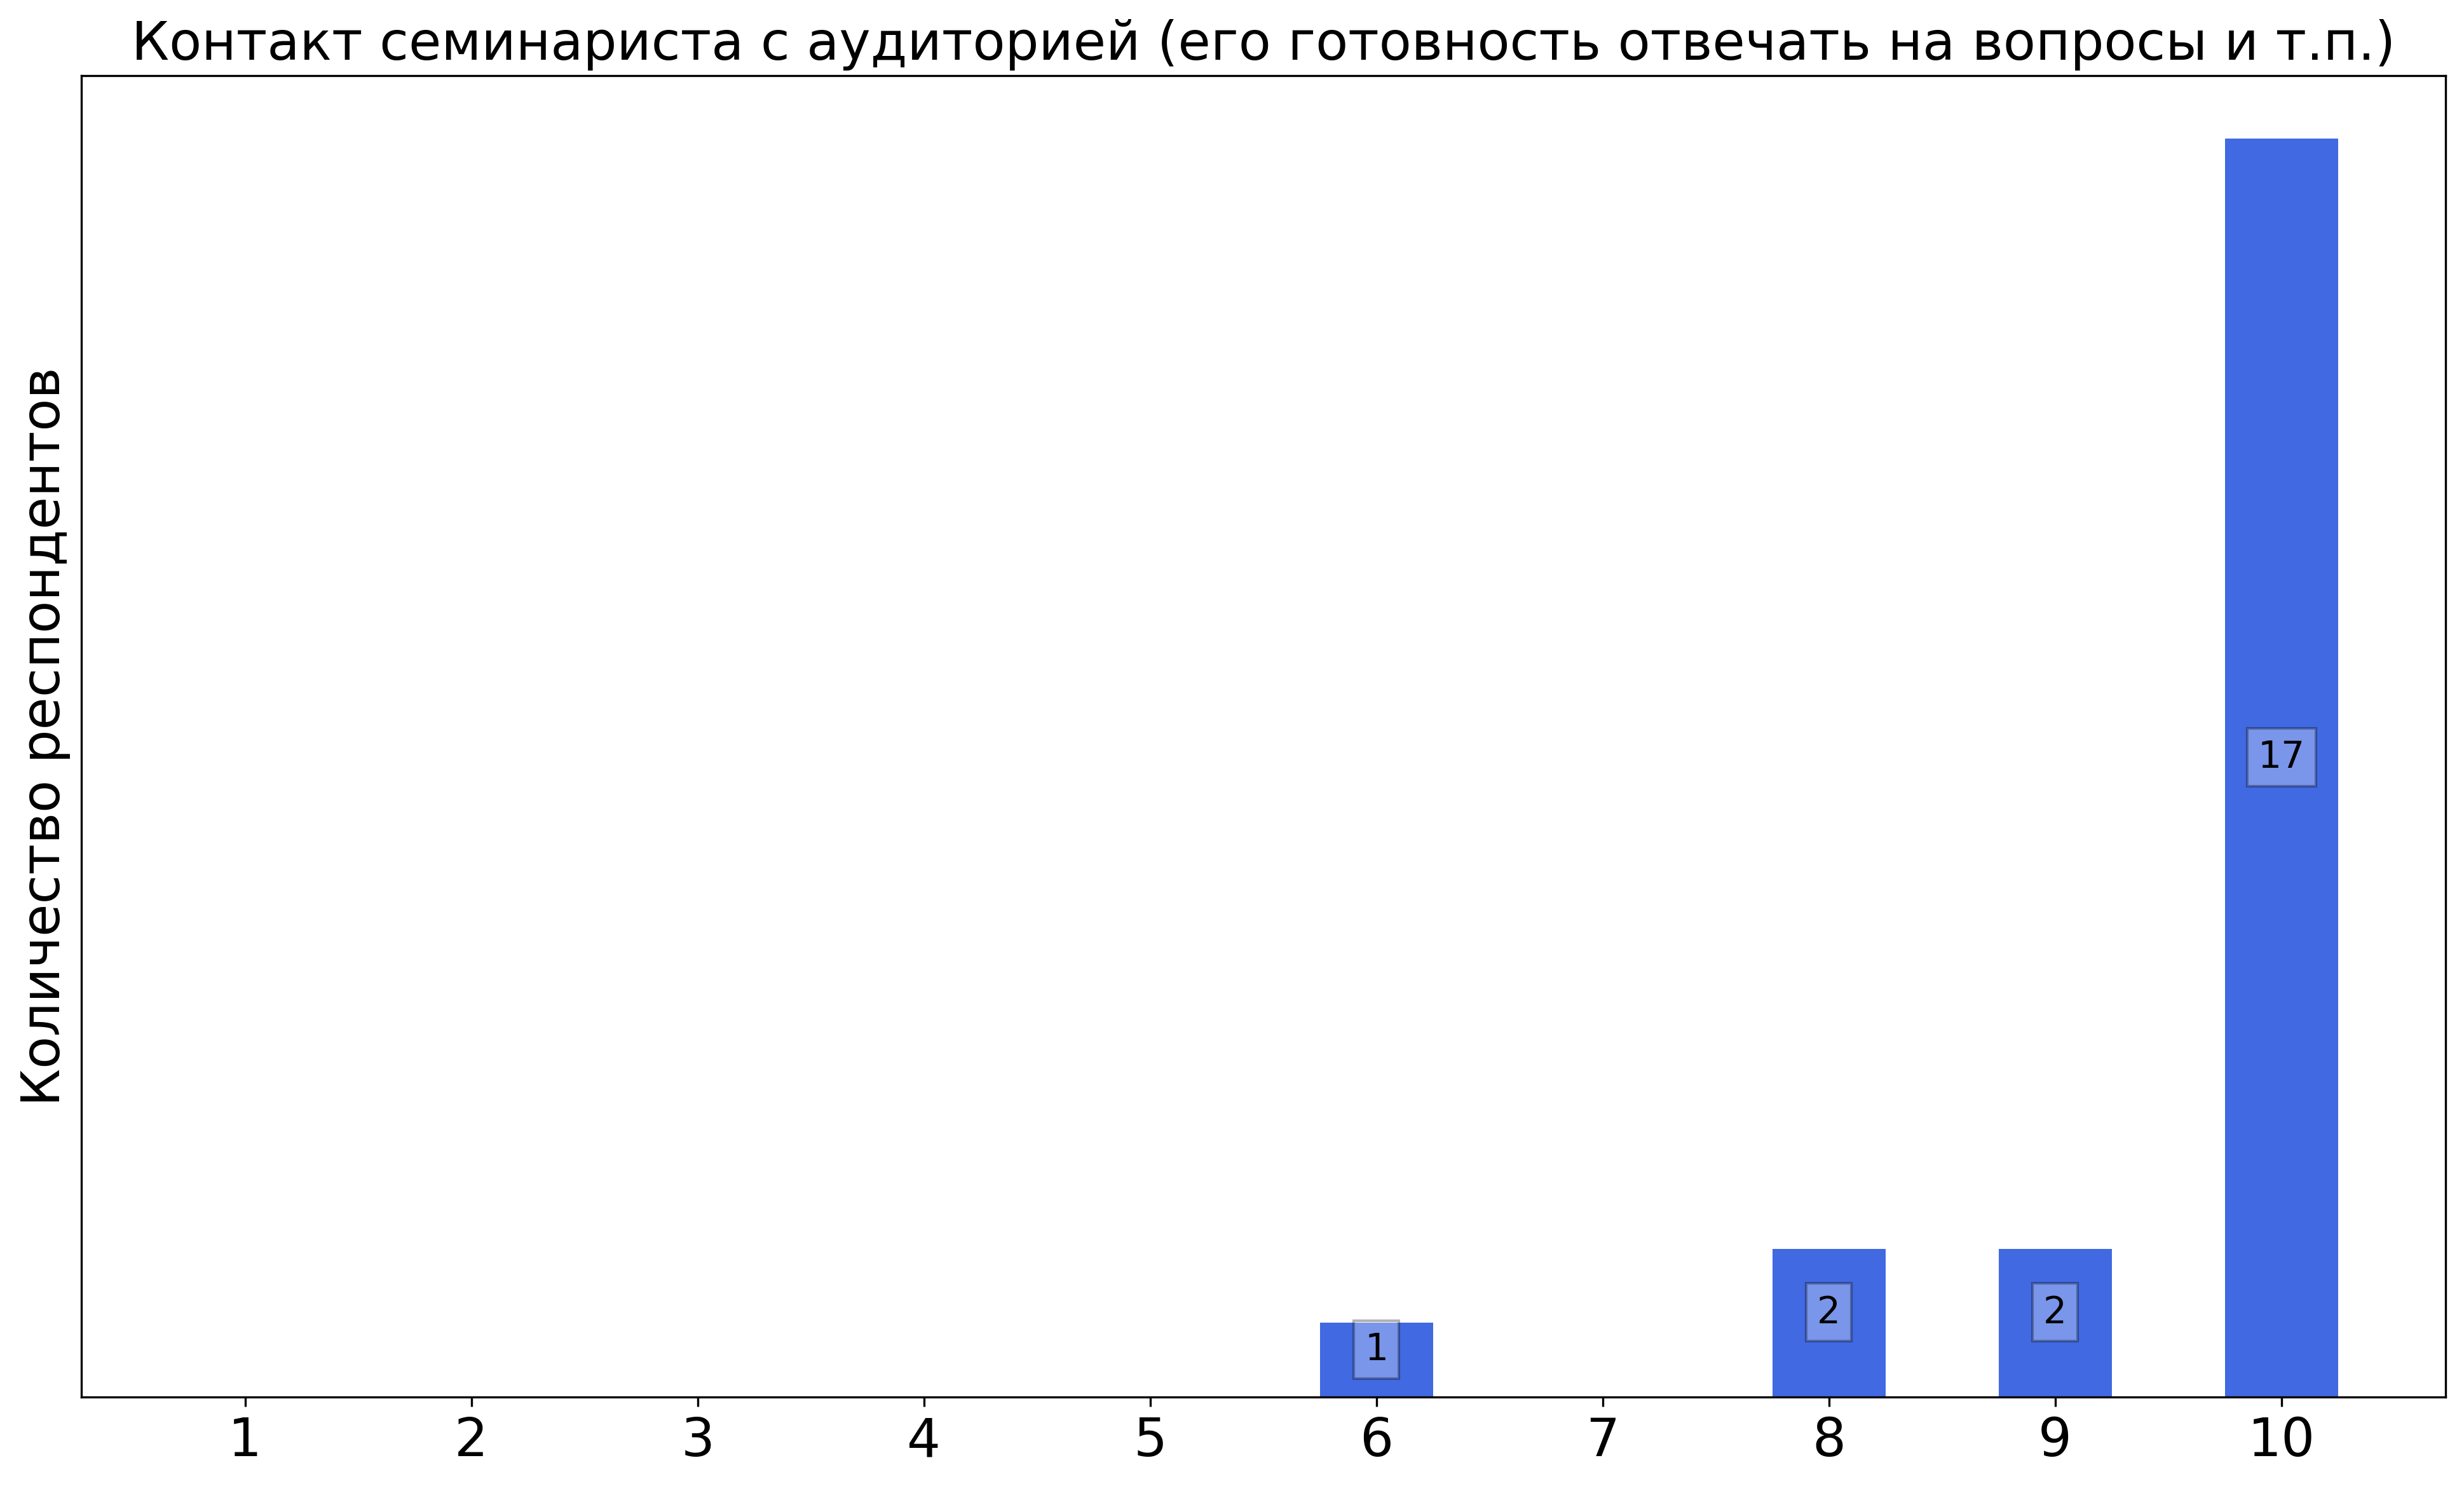
\includegraphics[width=\textwidth]{images/3 course/Теория поля/seminarists-marks-Дьяконов Д.В.-0.png}
            \end{subfigure}
            \begin{subfigure}[b]{0.45\textwidth}
                \centering
                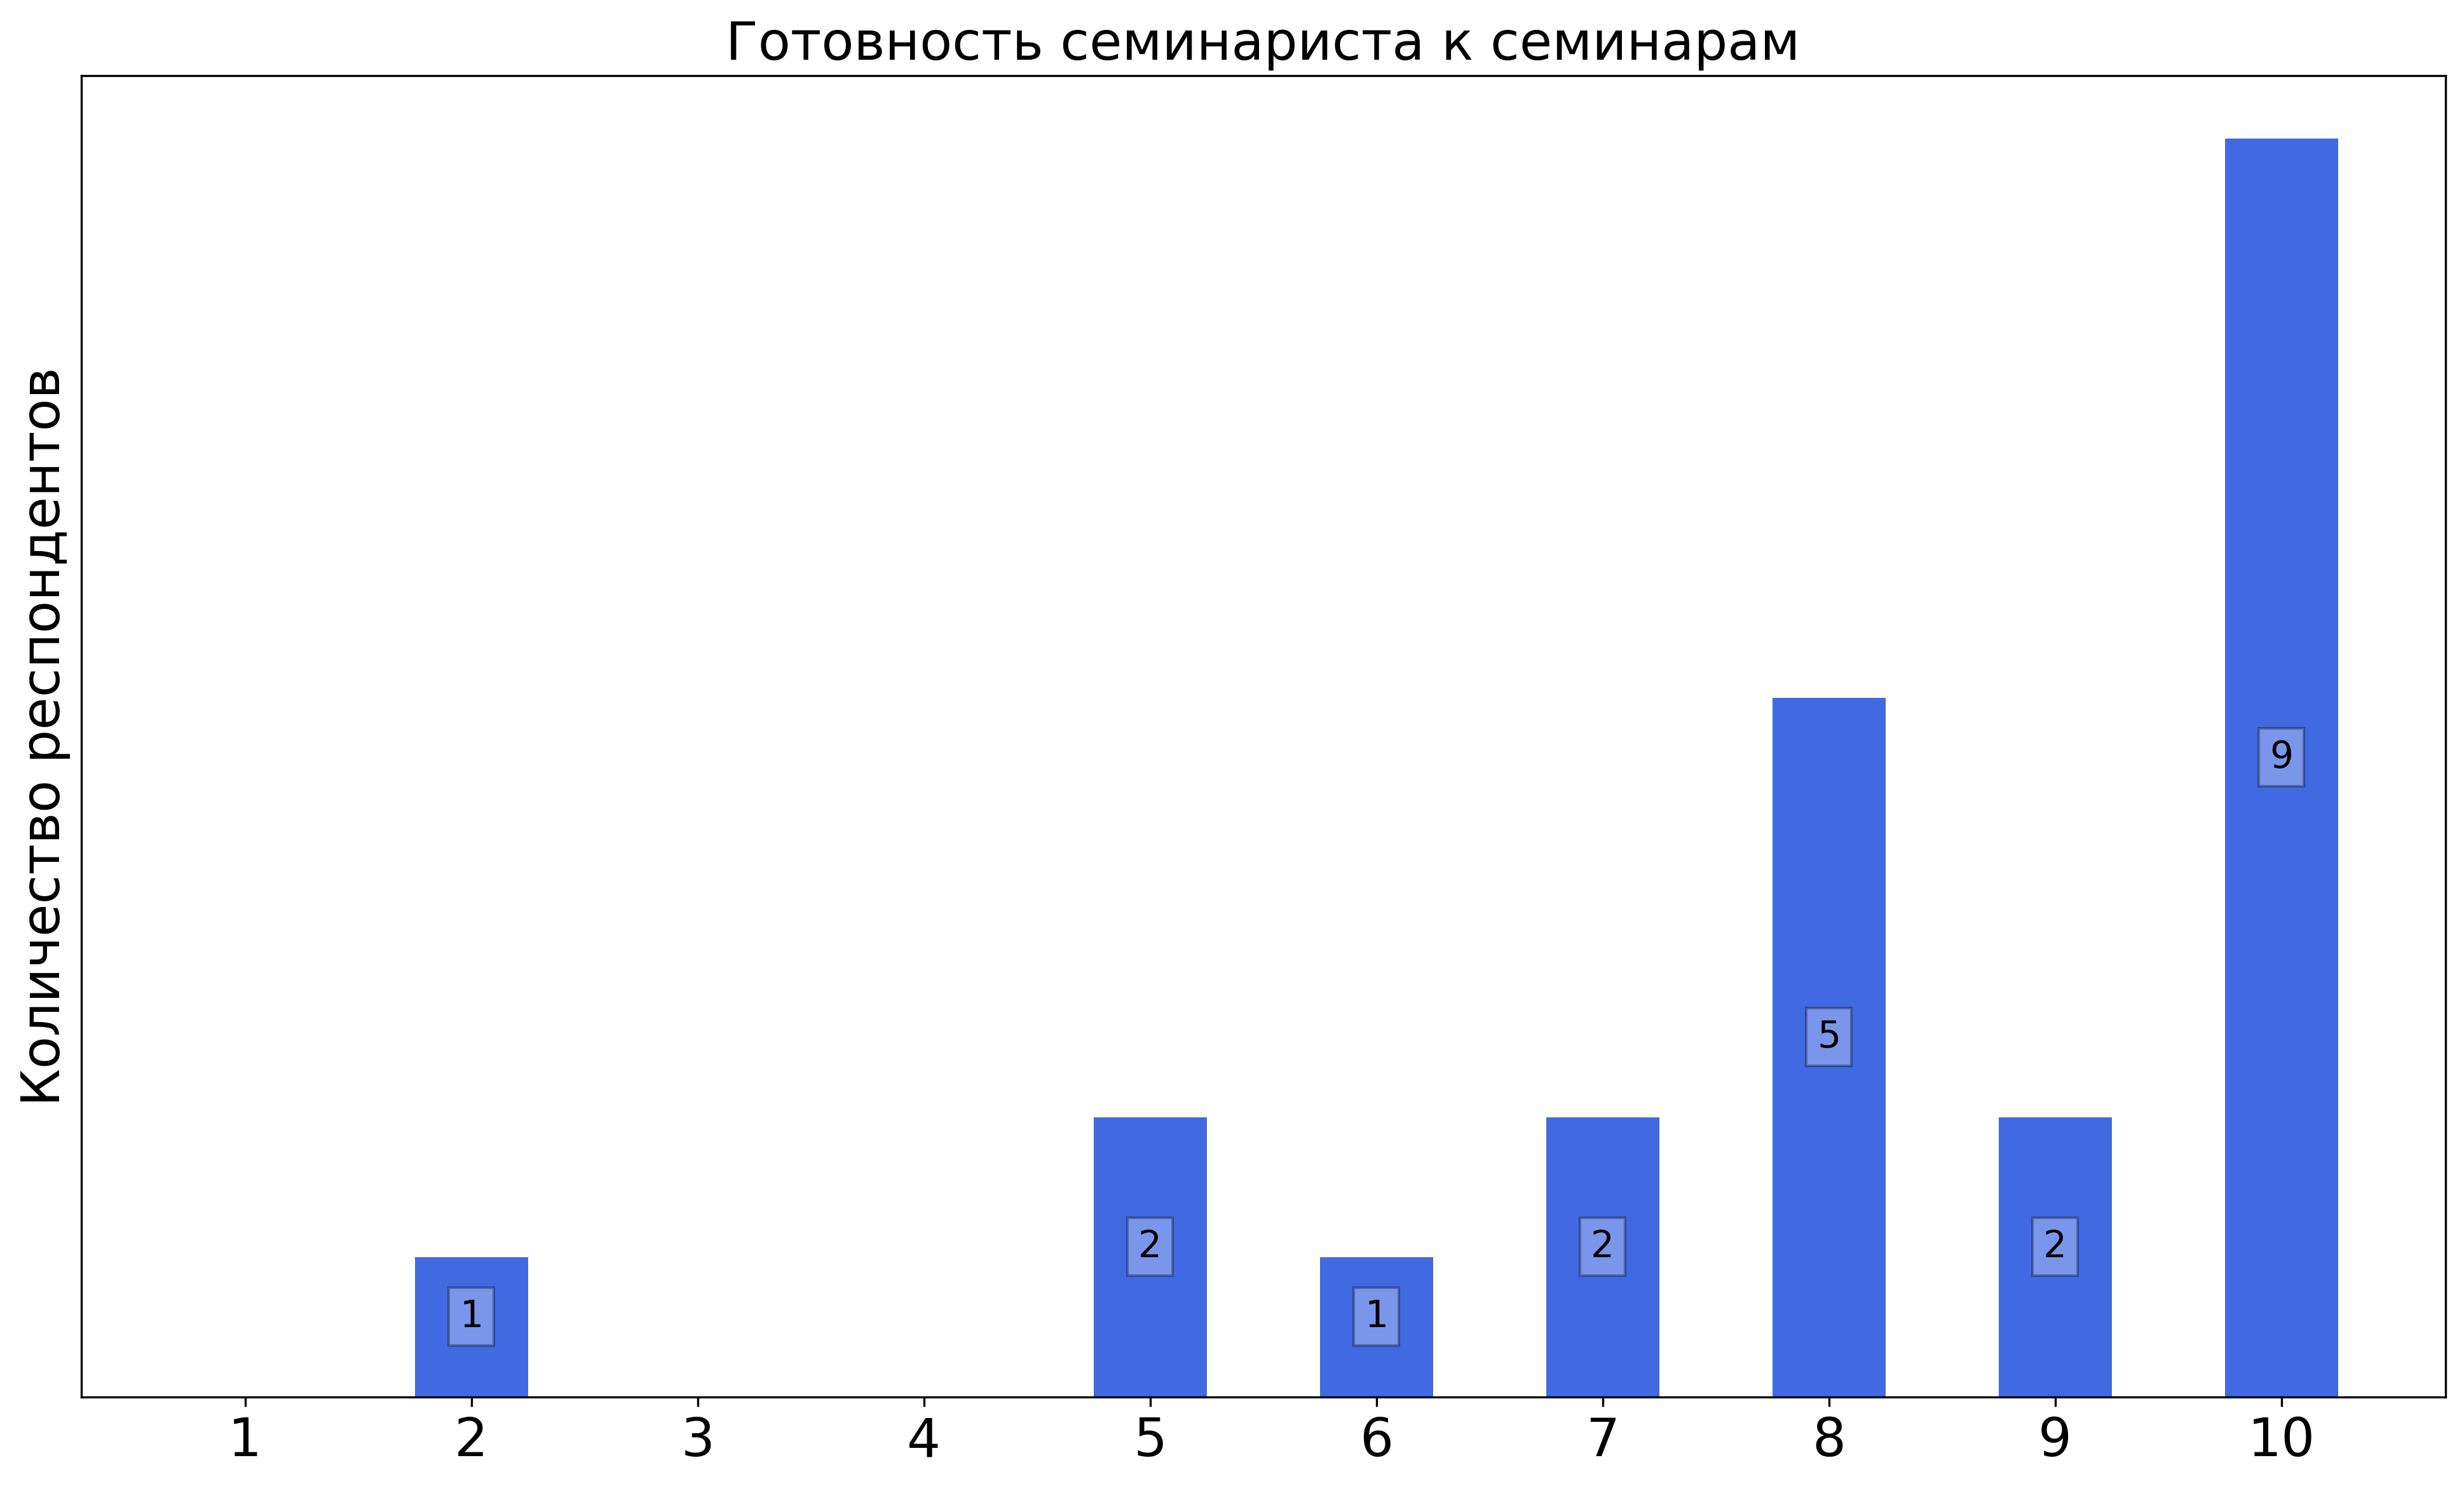
\includegraphics[width=\textwidth]{images/3 course/Теория поля/seminarists-marks-Дьяконов Д.В.-1.png}
            \end{subfigure}
            \begin{subfigure}[b]{0.45\textwidth}
                \centering
                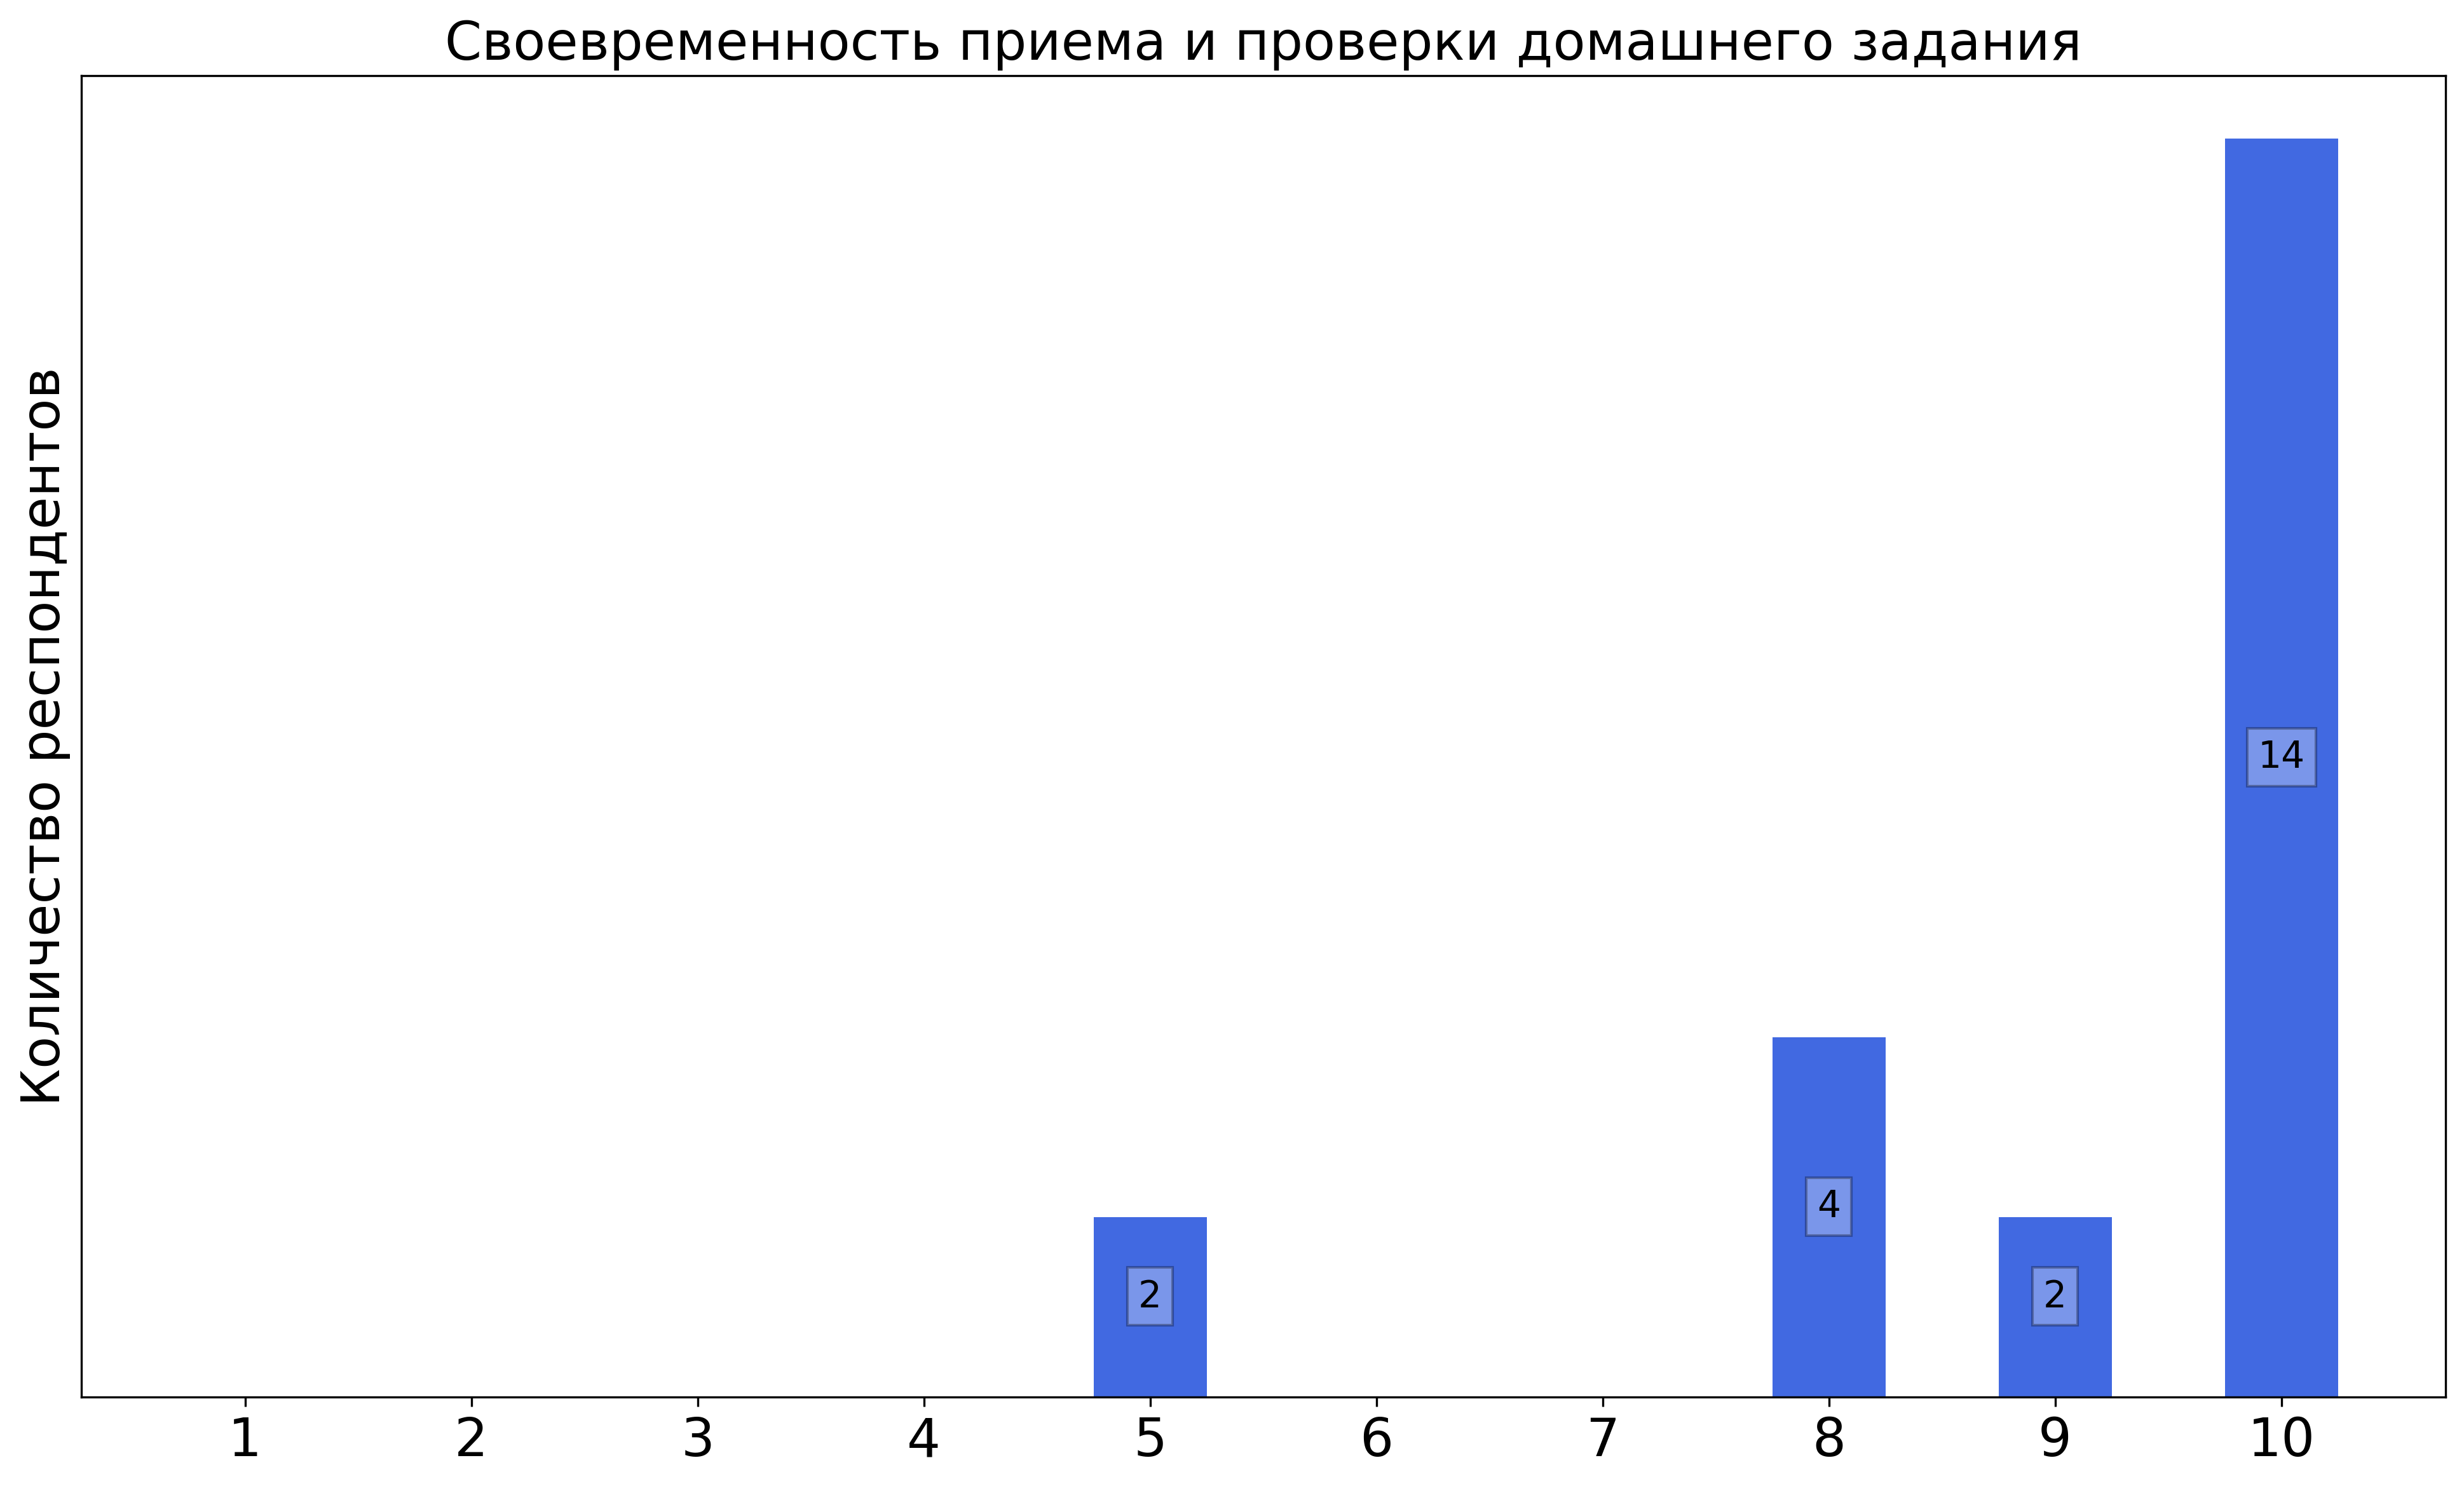
\includegraphics[width=\textwidth]{images/3 course/Теория поля/seminarists-marks-Дьяконов Д.В.-2.png}
            \end{subfigure}
            \begin{subfigure}[b]{0.45\textwidth}
                \centering
                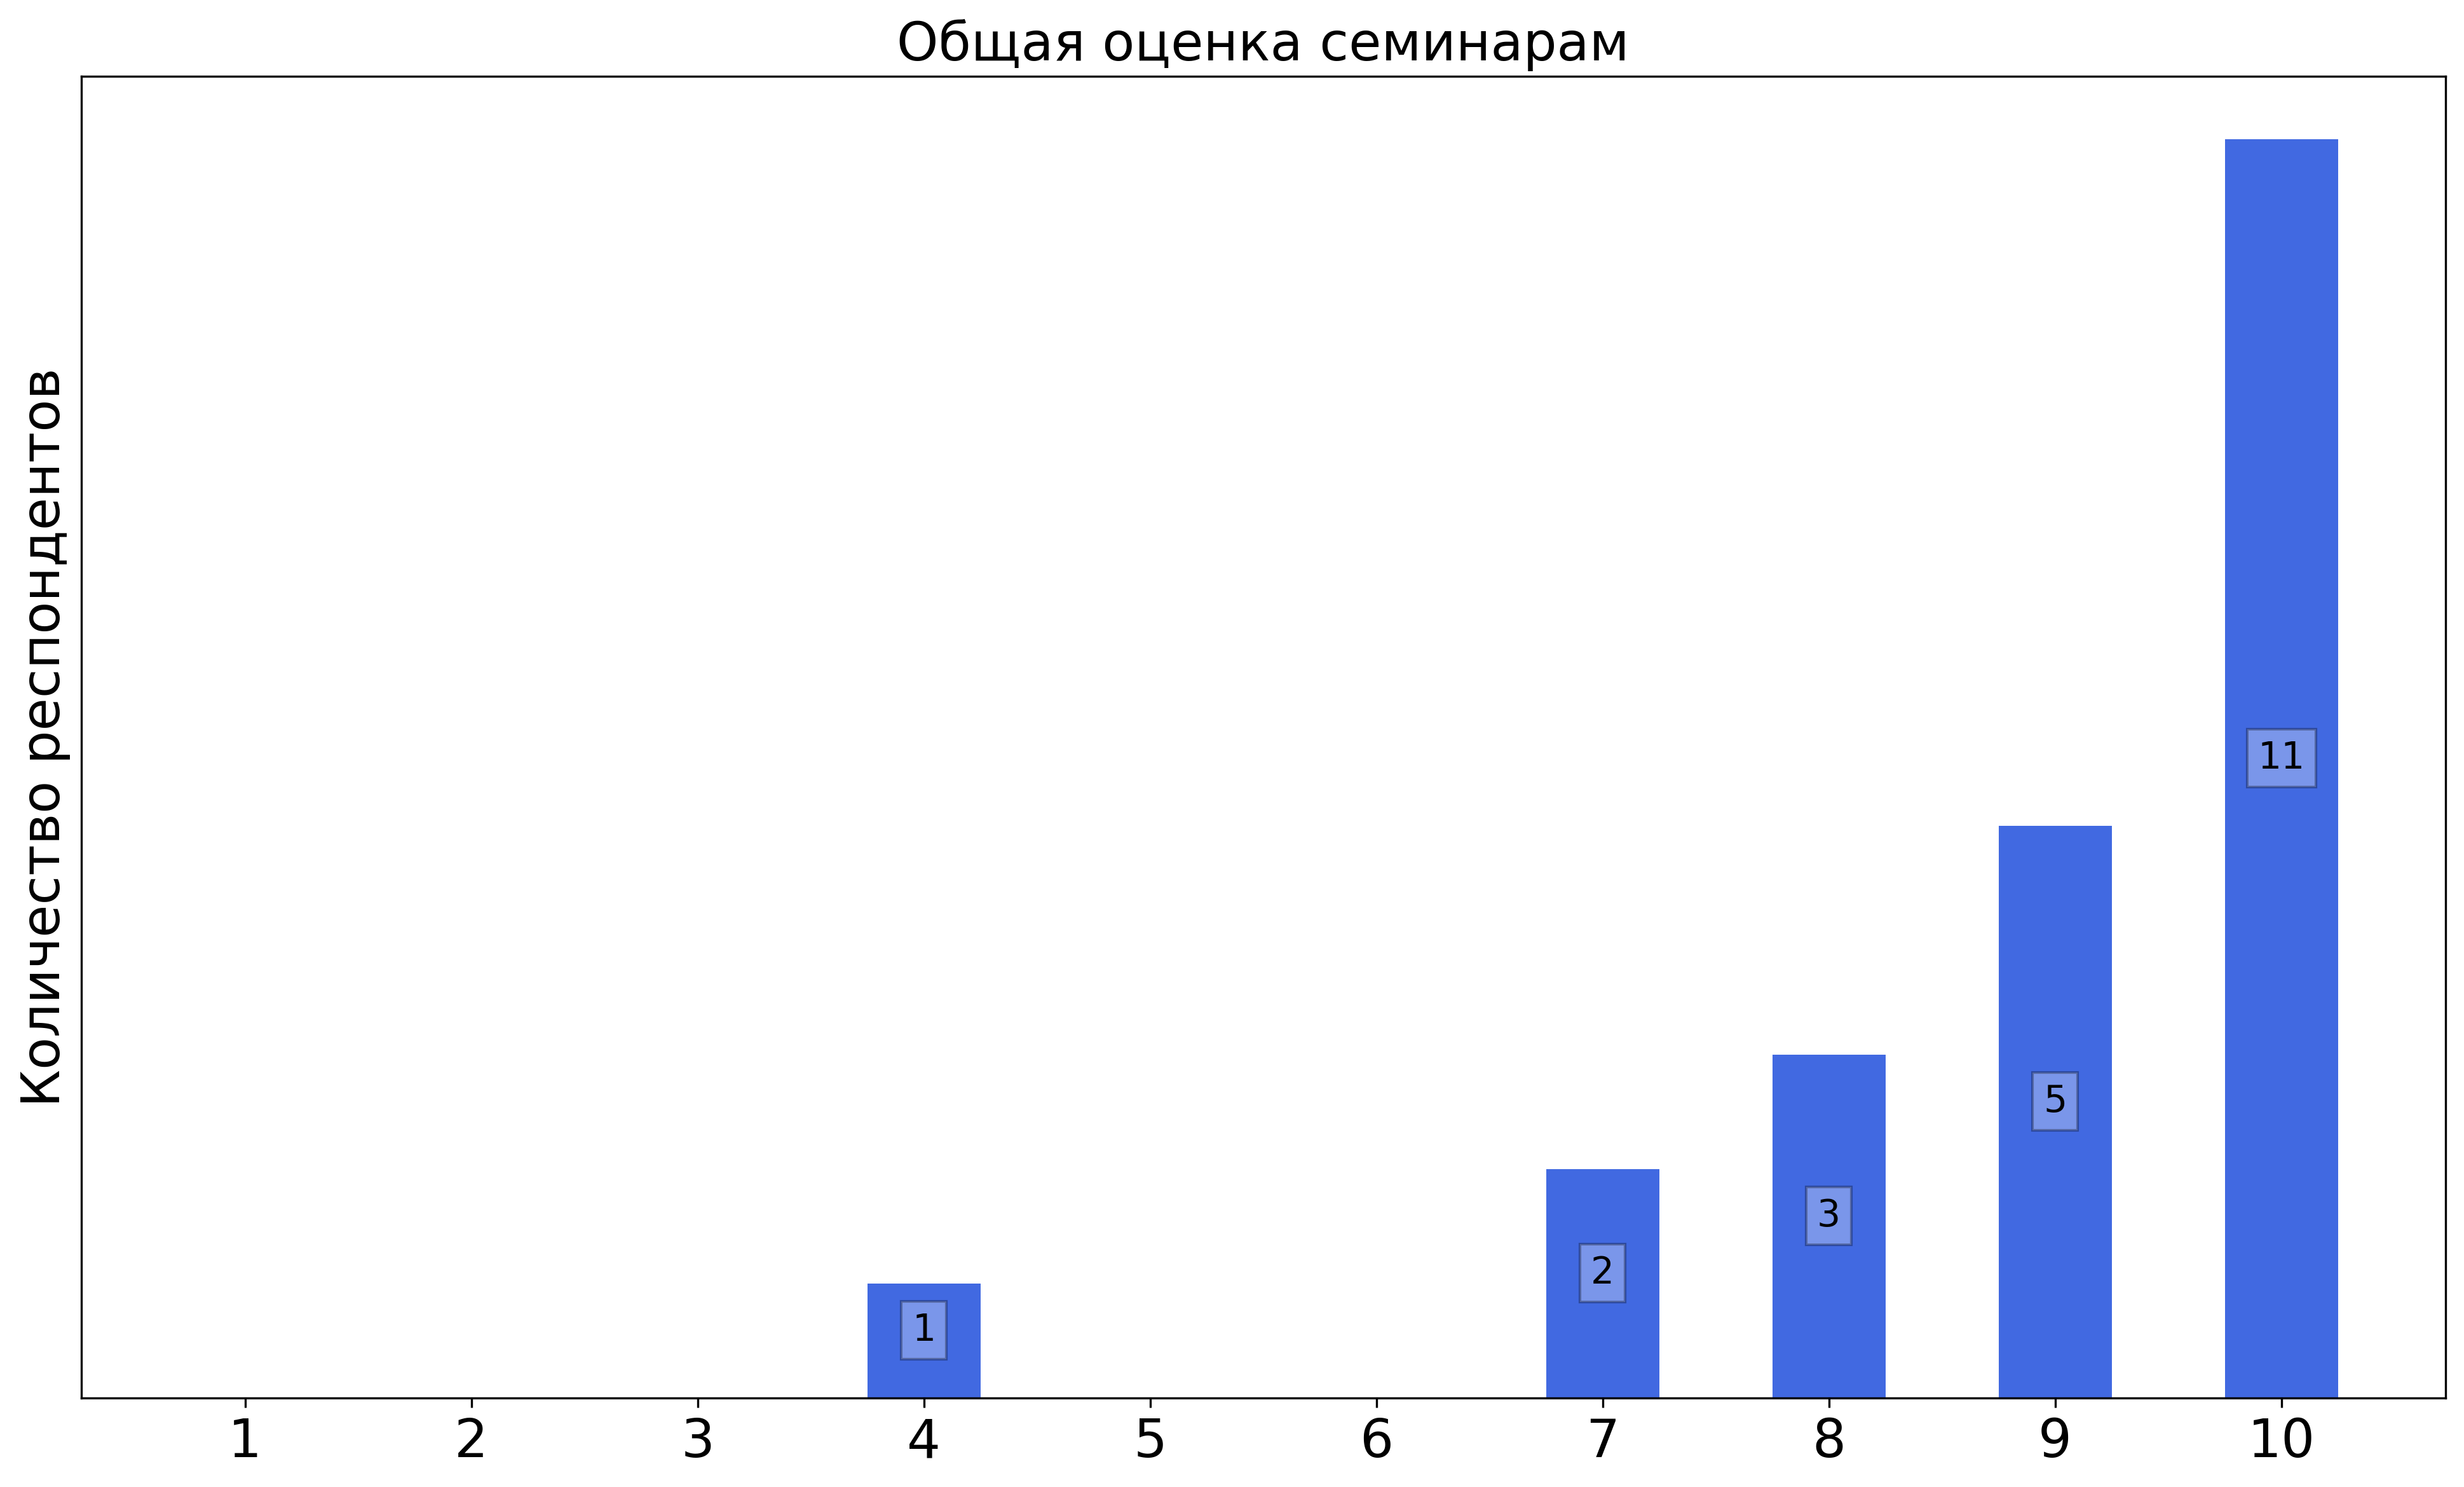
\includegraphics[width=\textwidth]{images/3 course/Теория поля/seminarists-marks-Дьяконов Д.В.-3.png}
            \end{subfigure}	
            \caption{Оценки респондентов о качестве преподавания семинаров}
        \end{figure}

        \textbf{Комментарии студентов о семинаристе\protect\footnote{сохранены оригинальные орфография и пунктуация}}
        \begin{commentbox} 
            Хороший вариант, если нужна халява. Семинары плохие: семинарист к ним не готовится и импровизирует. По итогу получается полная неразбериха, которую тяжело воспринимать 
        \end{commentbox} 
    
        \begin{commentbox} 
            Не хватает немного структуры, но ооочень приятен, знает предмет и любит его
        \end{commentbox} 
    
        \begin{commentbox} 
            Классный мужик. Круто рассказывает. Все понятно и интересно. Быстро и чётко принимает задание, оценкой не обижает, спасибо ему за этот семестр. 
        \end{commentbox} 
    
        \begin{commentbox} 
            Плохо доносит материал, не всегда успешно  отвечает на вопросы. Однако очень приятен в общении, почти каждый день доступен для сдачи дз (работает в физтеховской лабе) и принимает ее досконально, заставляя самому разобраться в вопросе, даже если только на следующий - в общем очень крутые сдачи позволяющие зашарить предмет. Также добрый, брсом не обидит
        \end{commentbox} 
    
        \begin{commentbox} 
            Рассказывает максимально понятно. Сдачи заданий хоть каждую неделю (если есть что сдавать).  
        \end{commentbox} 
    
        \begin{commentbox} 
            Хороший семинарист, хорошо взаимодействует со студентами, суть семинаров - разобраться в материале, а не просто решить задачки, что делает семинары очень продуктивными, даже если что-то не доразбиралось. 
        \end{commentbox} 
    
        \begin{commentbox} 
            Семинарист классный, но непунктуальный и часто переносящий встречи в последний момент 
        \end{commentbox} 
    
        \begin{commentbox} 
            Очень хороший семинарист. 
        \end{commentbox} 
    
        \begin{commentbox} 
            Семинары не очень структурированные, разбирается немного задач, записи на доске ведутся коряво и не полно. 
        \end{commentbox} 
    
        \begin{commentbox} 
            Очень классный семинарист, любит свой предмет. 
        \end{commentbox} 
    
        \begin{commentbox} 
            Семинарист 11/10, с пониманием относится к студентам, объясняет довольно быстро и бывает непонятно, но на вопросы всегда отвечает, в общении очень приятный. На сдачах задает базовые вопросы на понимание - то, что нужно. 
        \end{commentbox} 
    

    \subsubsection{Отзыв студентов о семинарах. Семинарист: Осипов Д.Л.}
		\begin{figure}[H]
			\centering
			\begin{subfigure}[b]{0.45\textwidth}
				\centering
				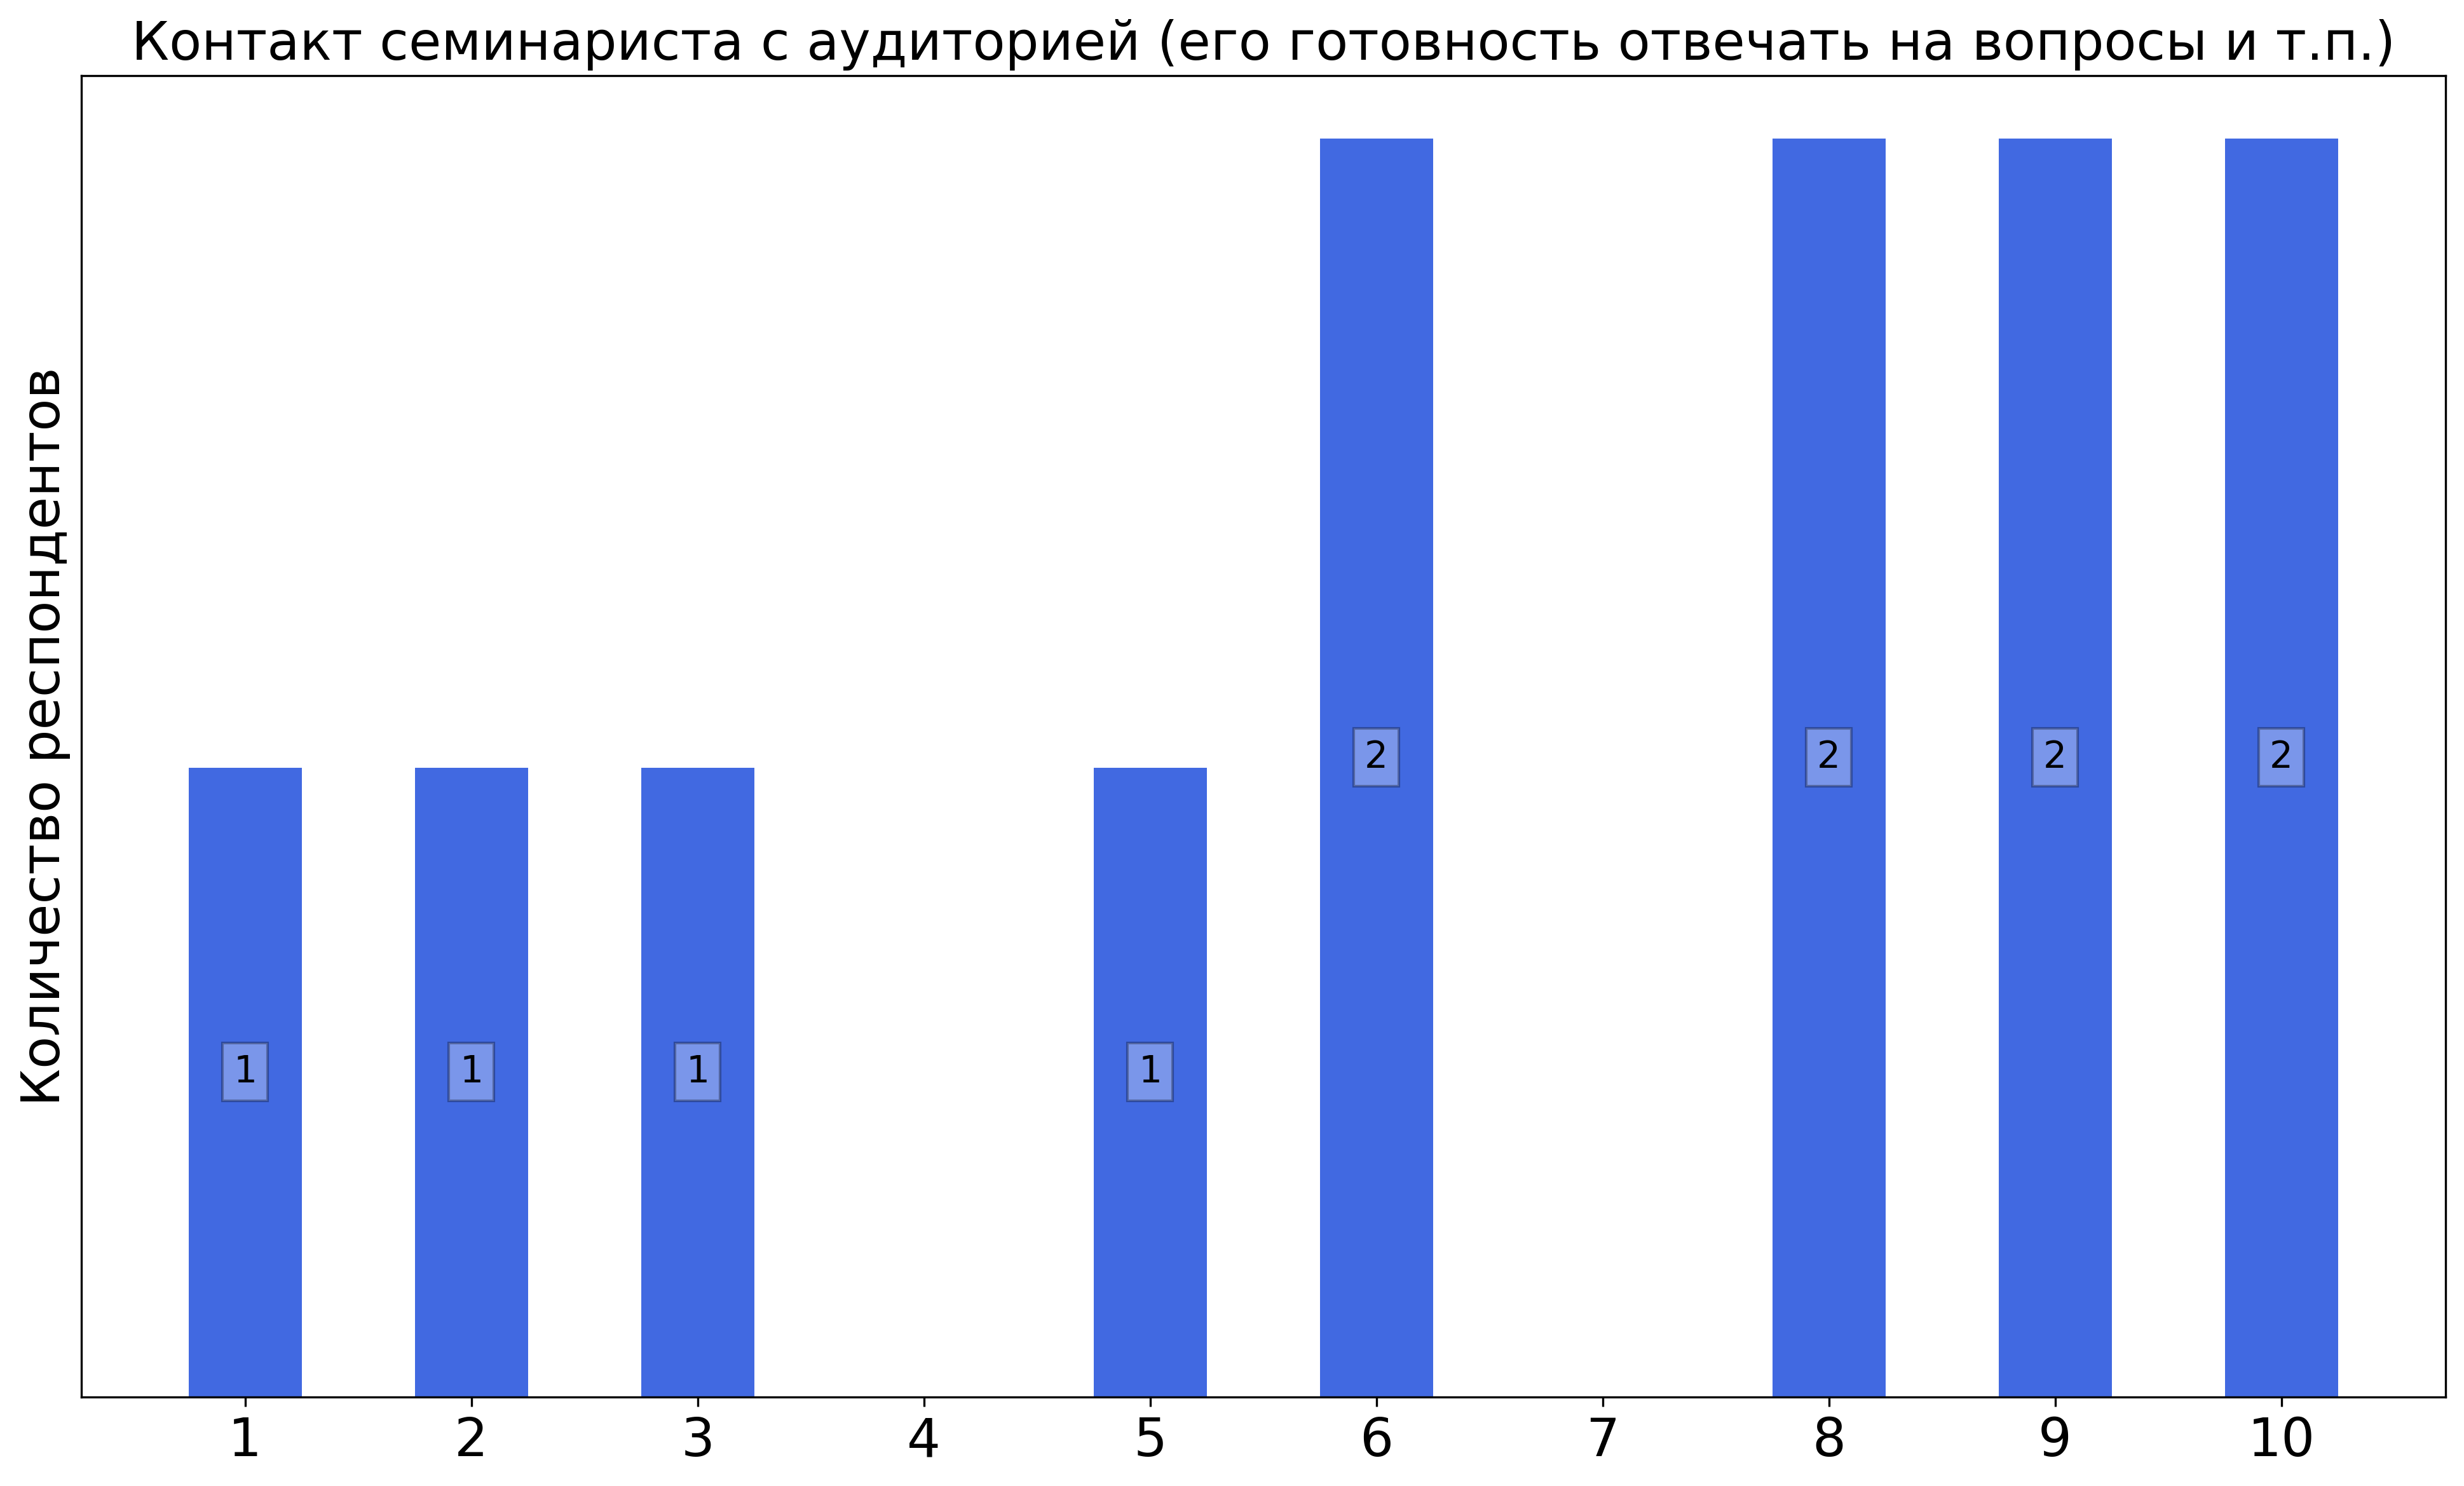
\includegraphics[width=\textwidth]{images/3 course/Теория поля/seminarists-marks-Осипов Д.Л.-0.png}
			\end{subfigure}
			\begin{subfigure}[b]{0.45\textwidth}
				\centering
				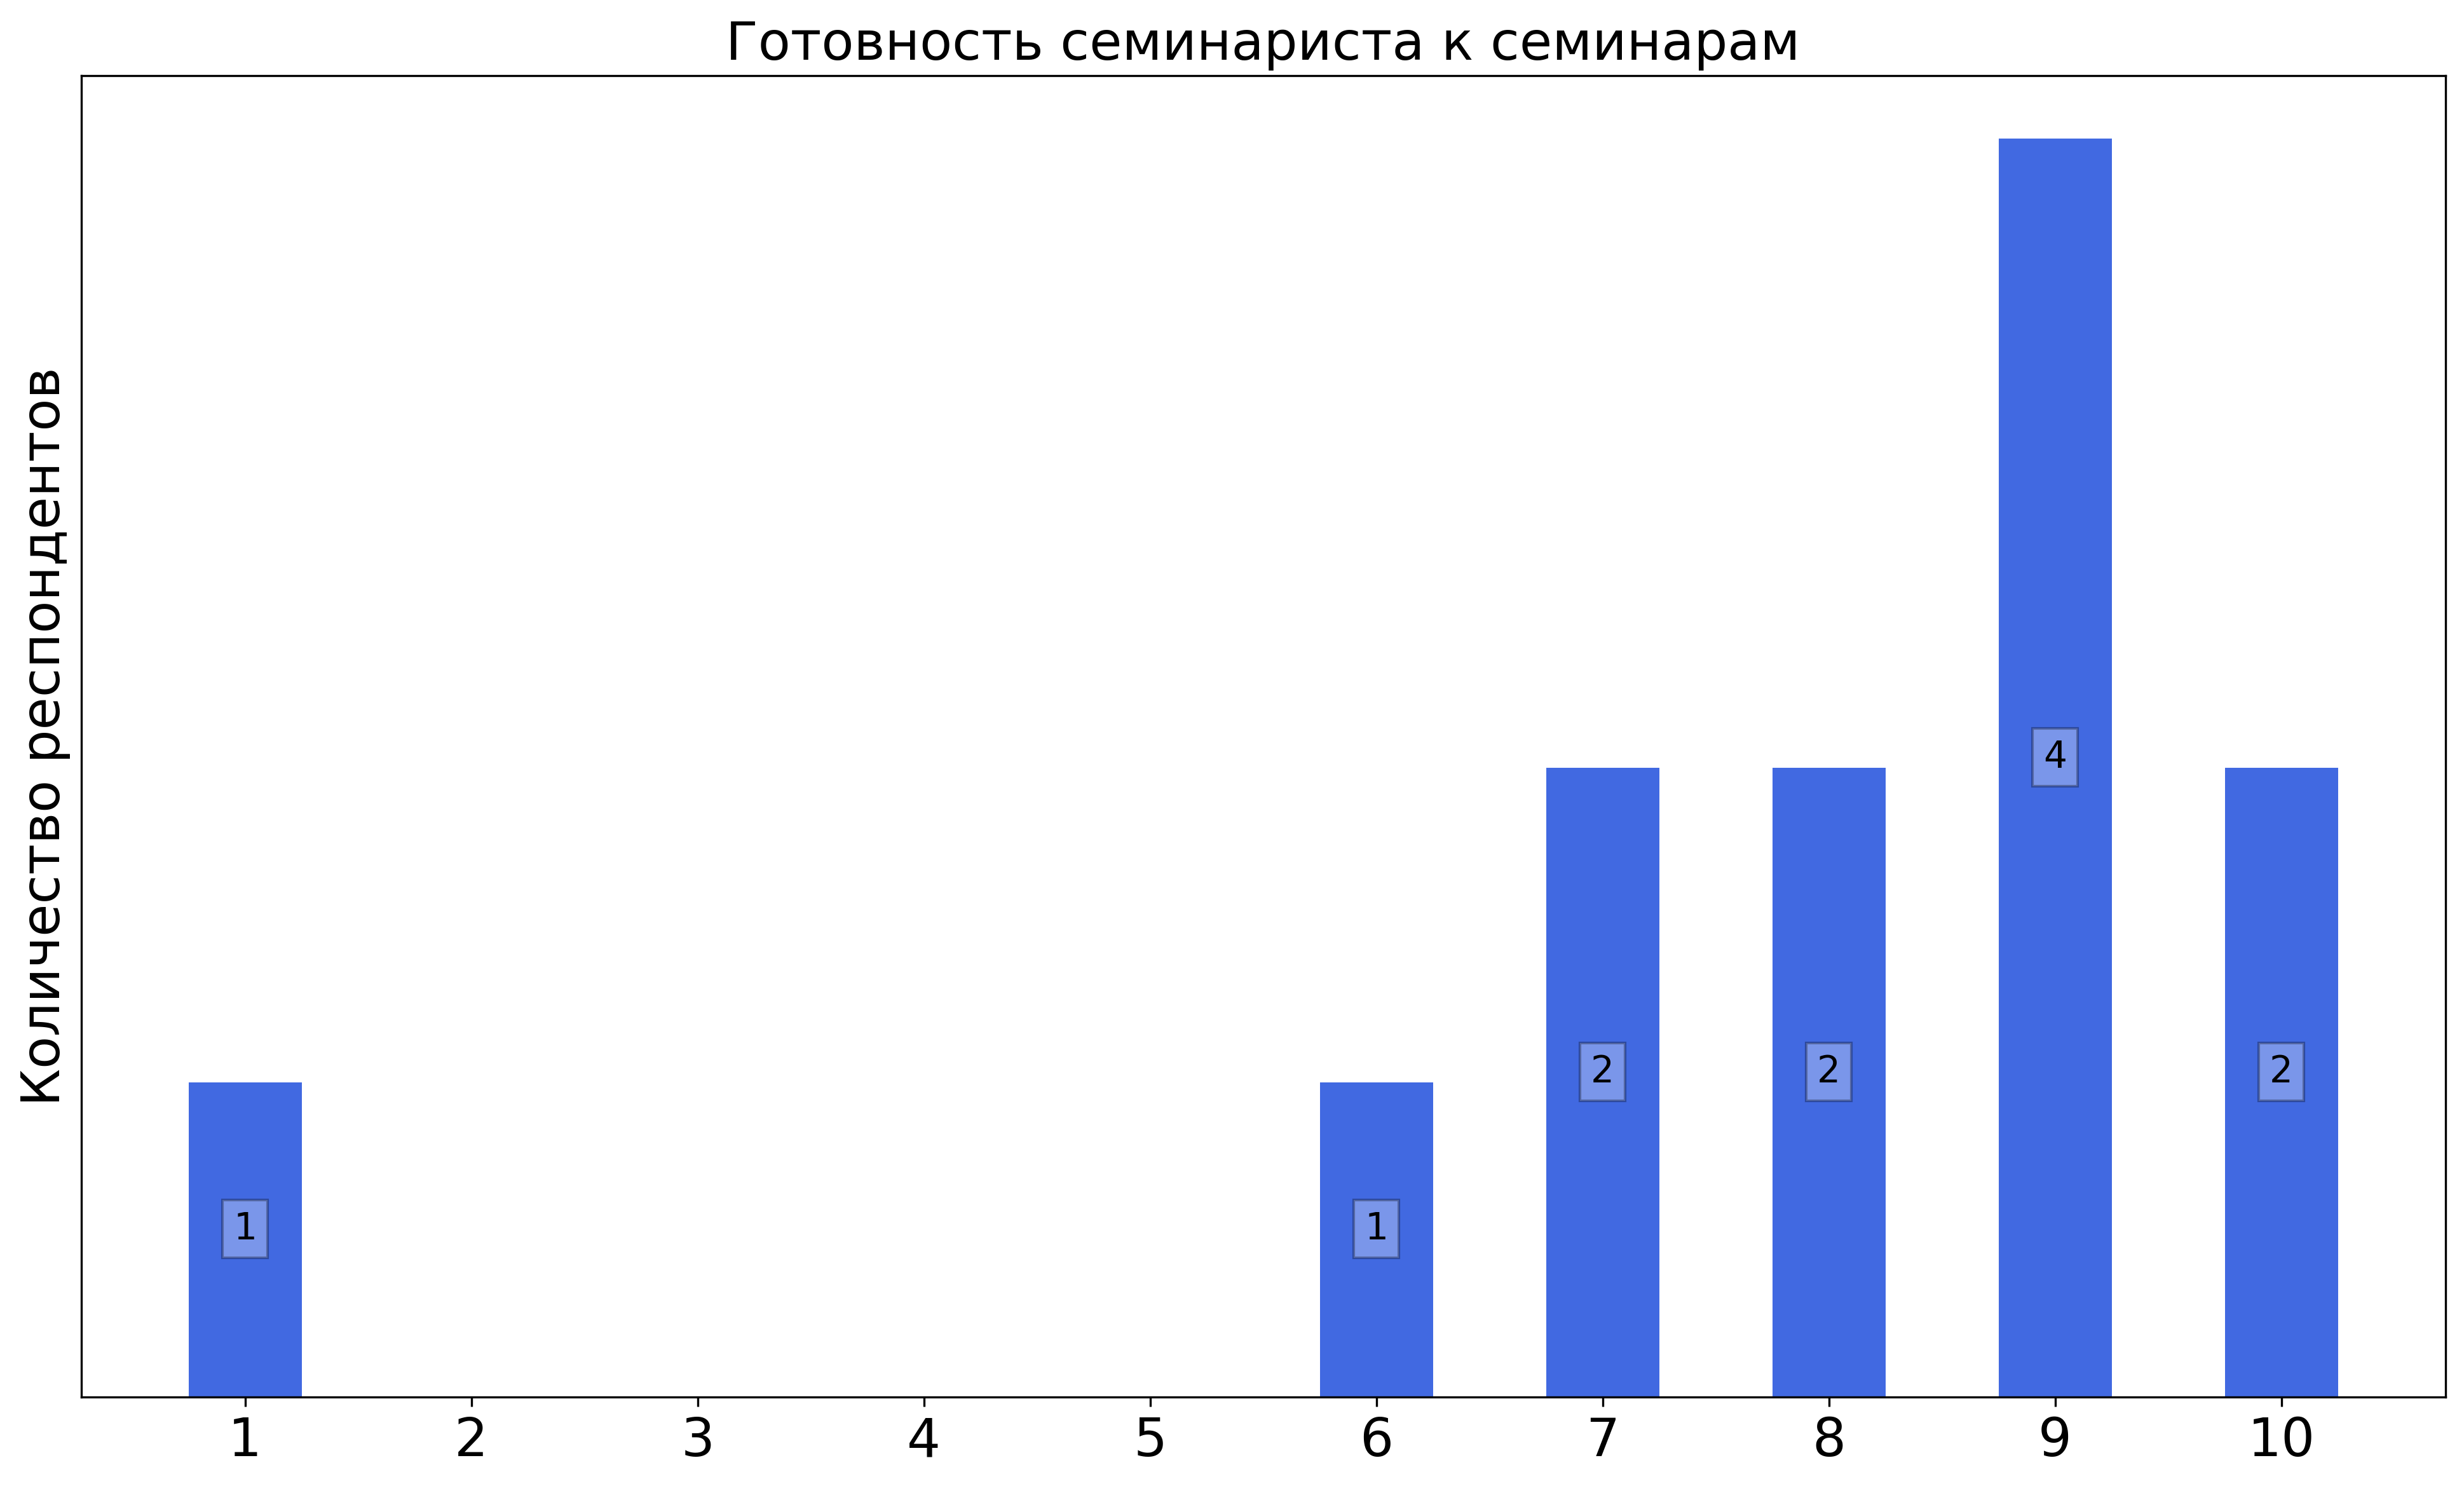
\includegraphics[width=\textwidth]{images/3 course/Теория поля/seminarists-marks-Осипов Д.Л.-1.png}
			\end{subfigure}
			\begin{subfigure}[b]{0.45\textwidth}
				\centering
				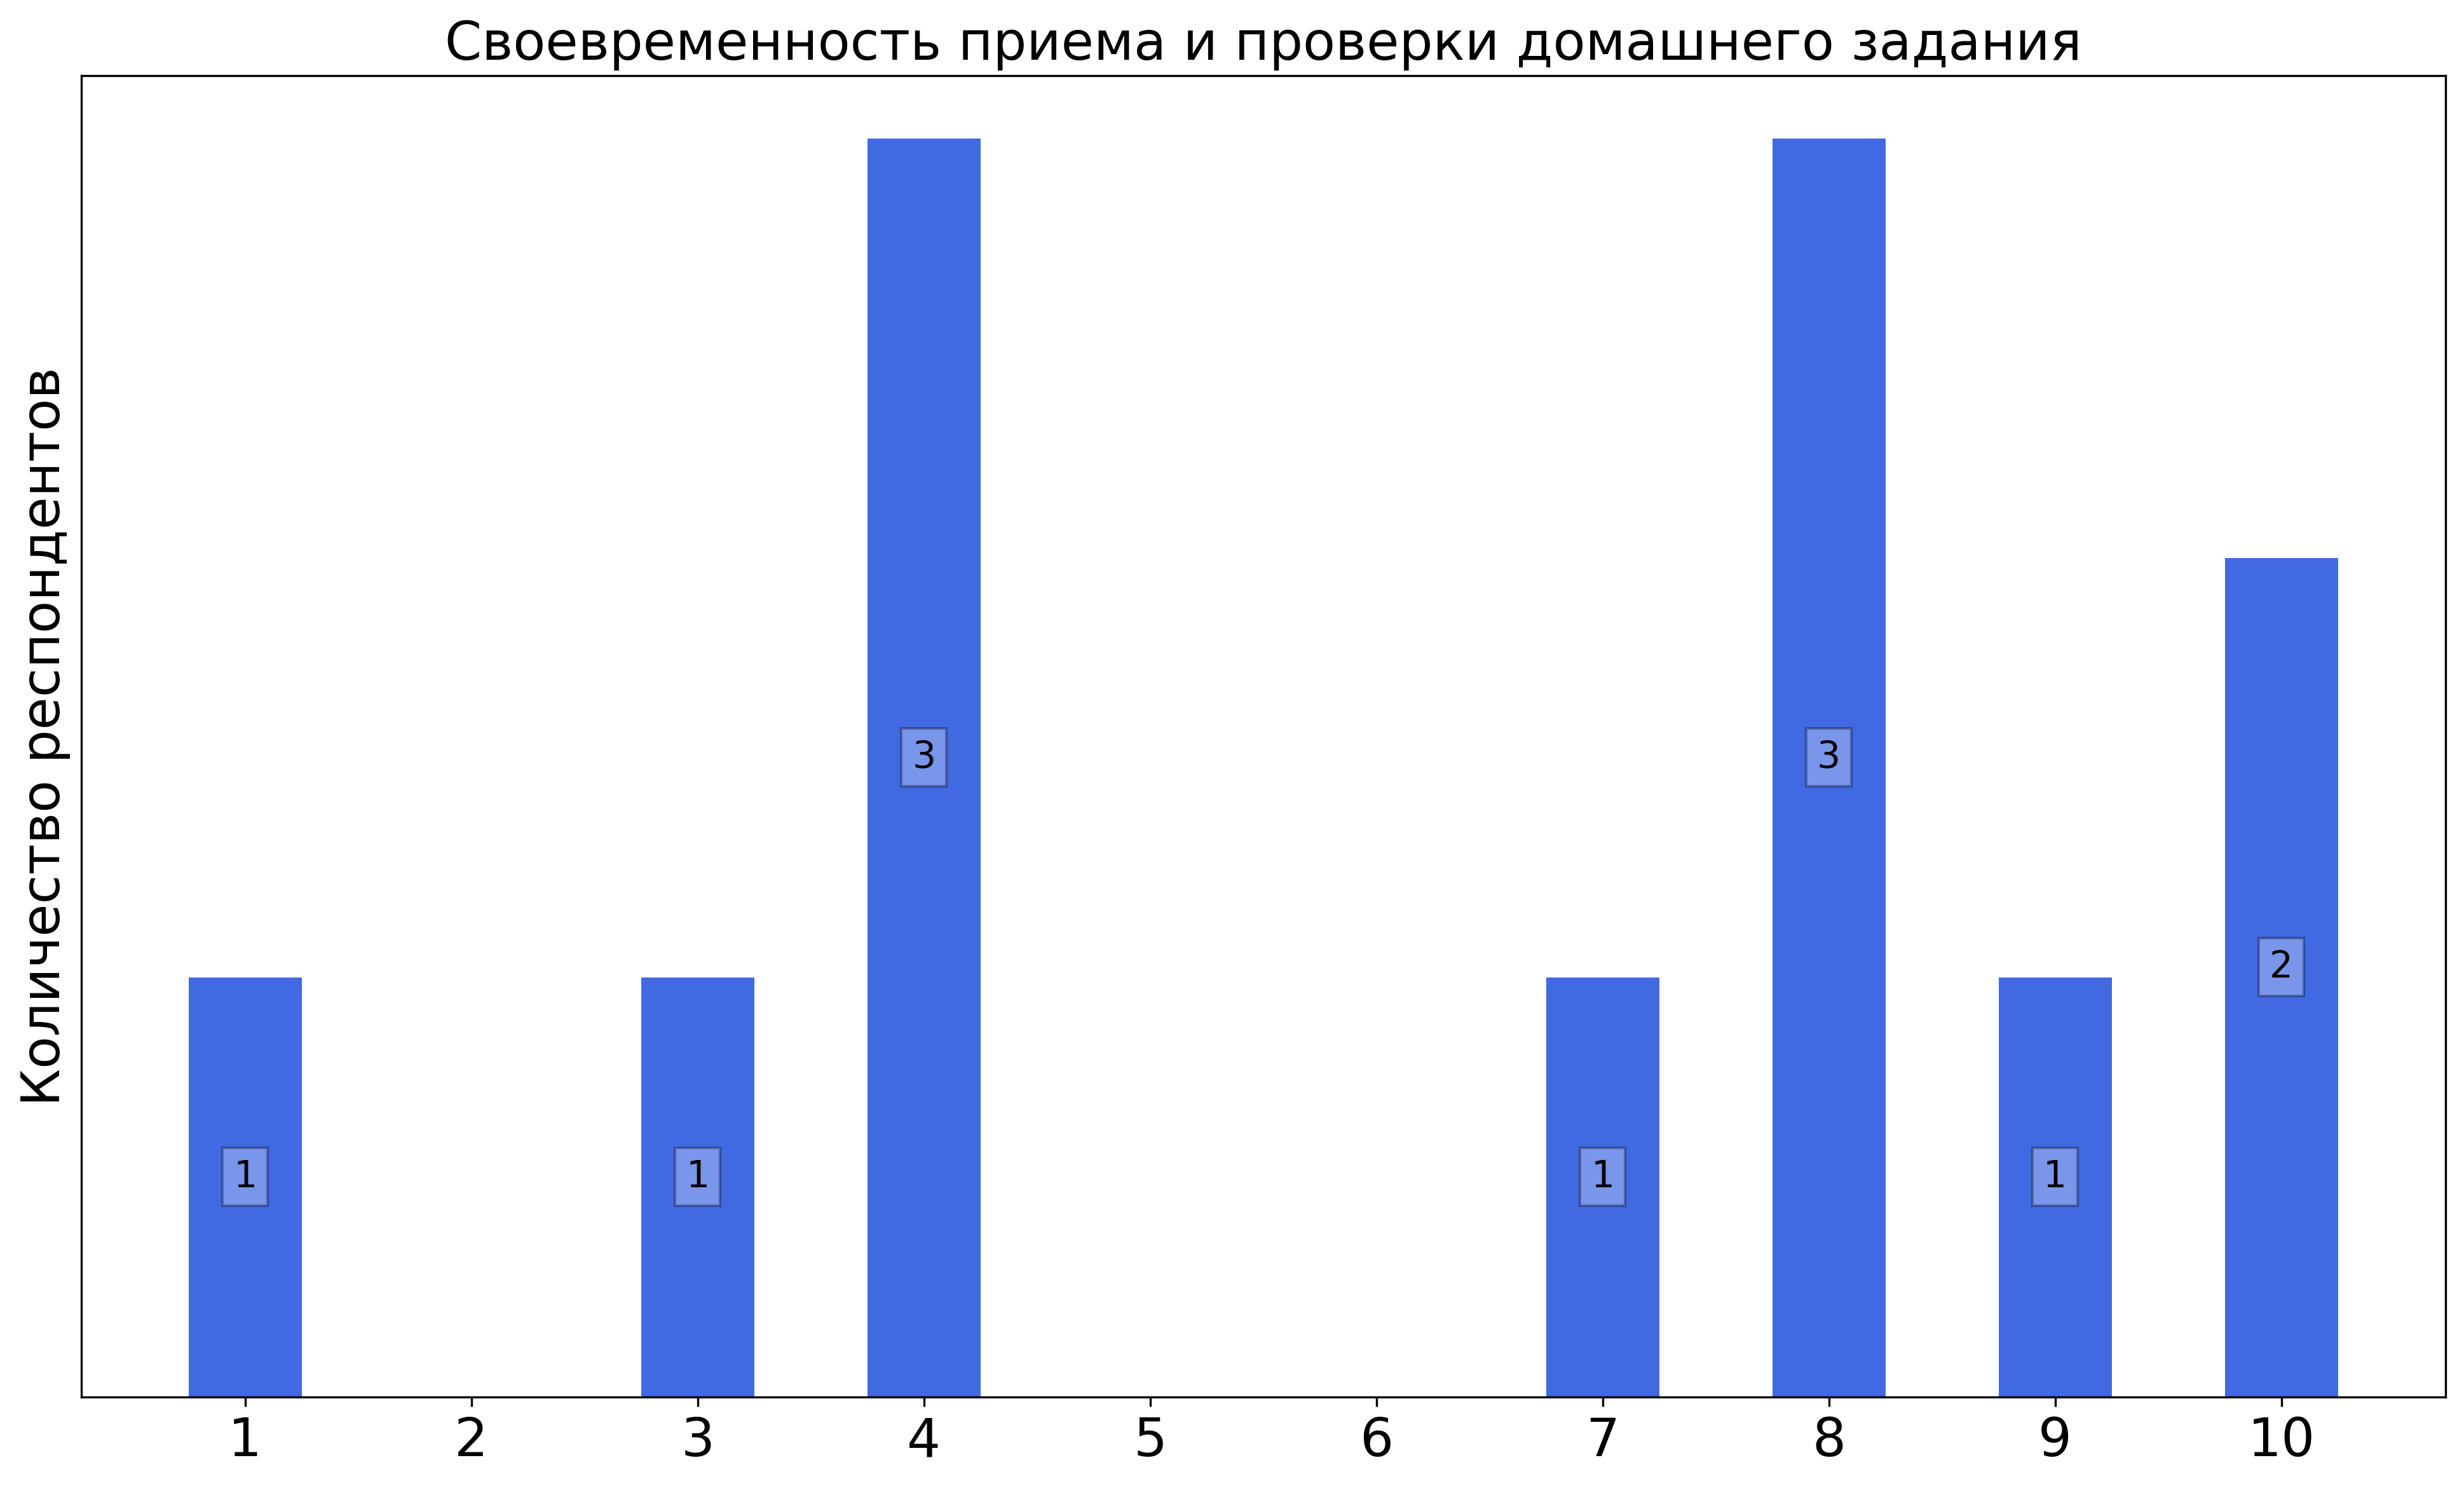
\includegraphics[width=\textwidth]{images/3 course/Теория поля/seminarists-marks-Осипов Д.Л.-2.png}
			\end{subfigure}
			\begin{subfigure}[b]{0.45\textwidth}
				\centering
				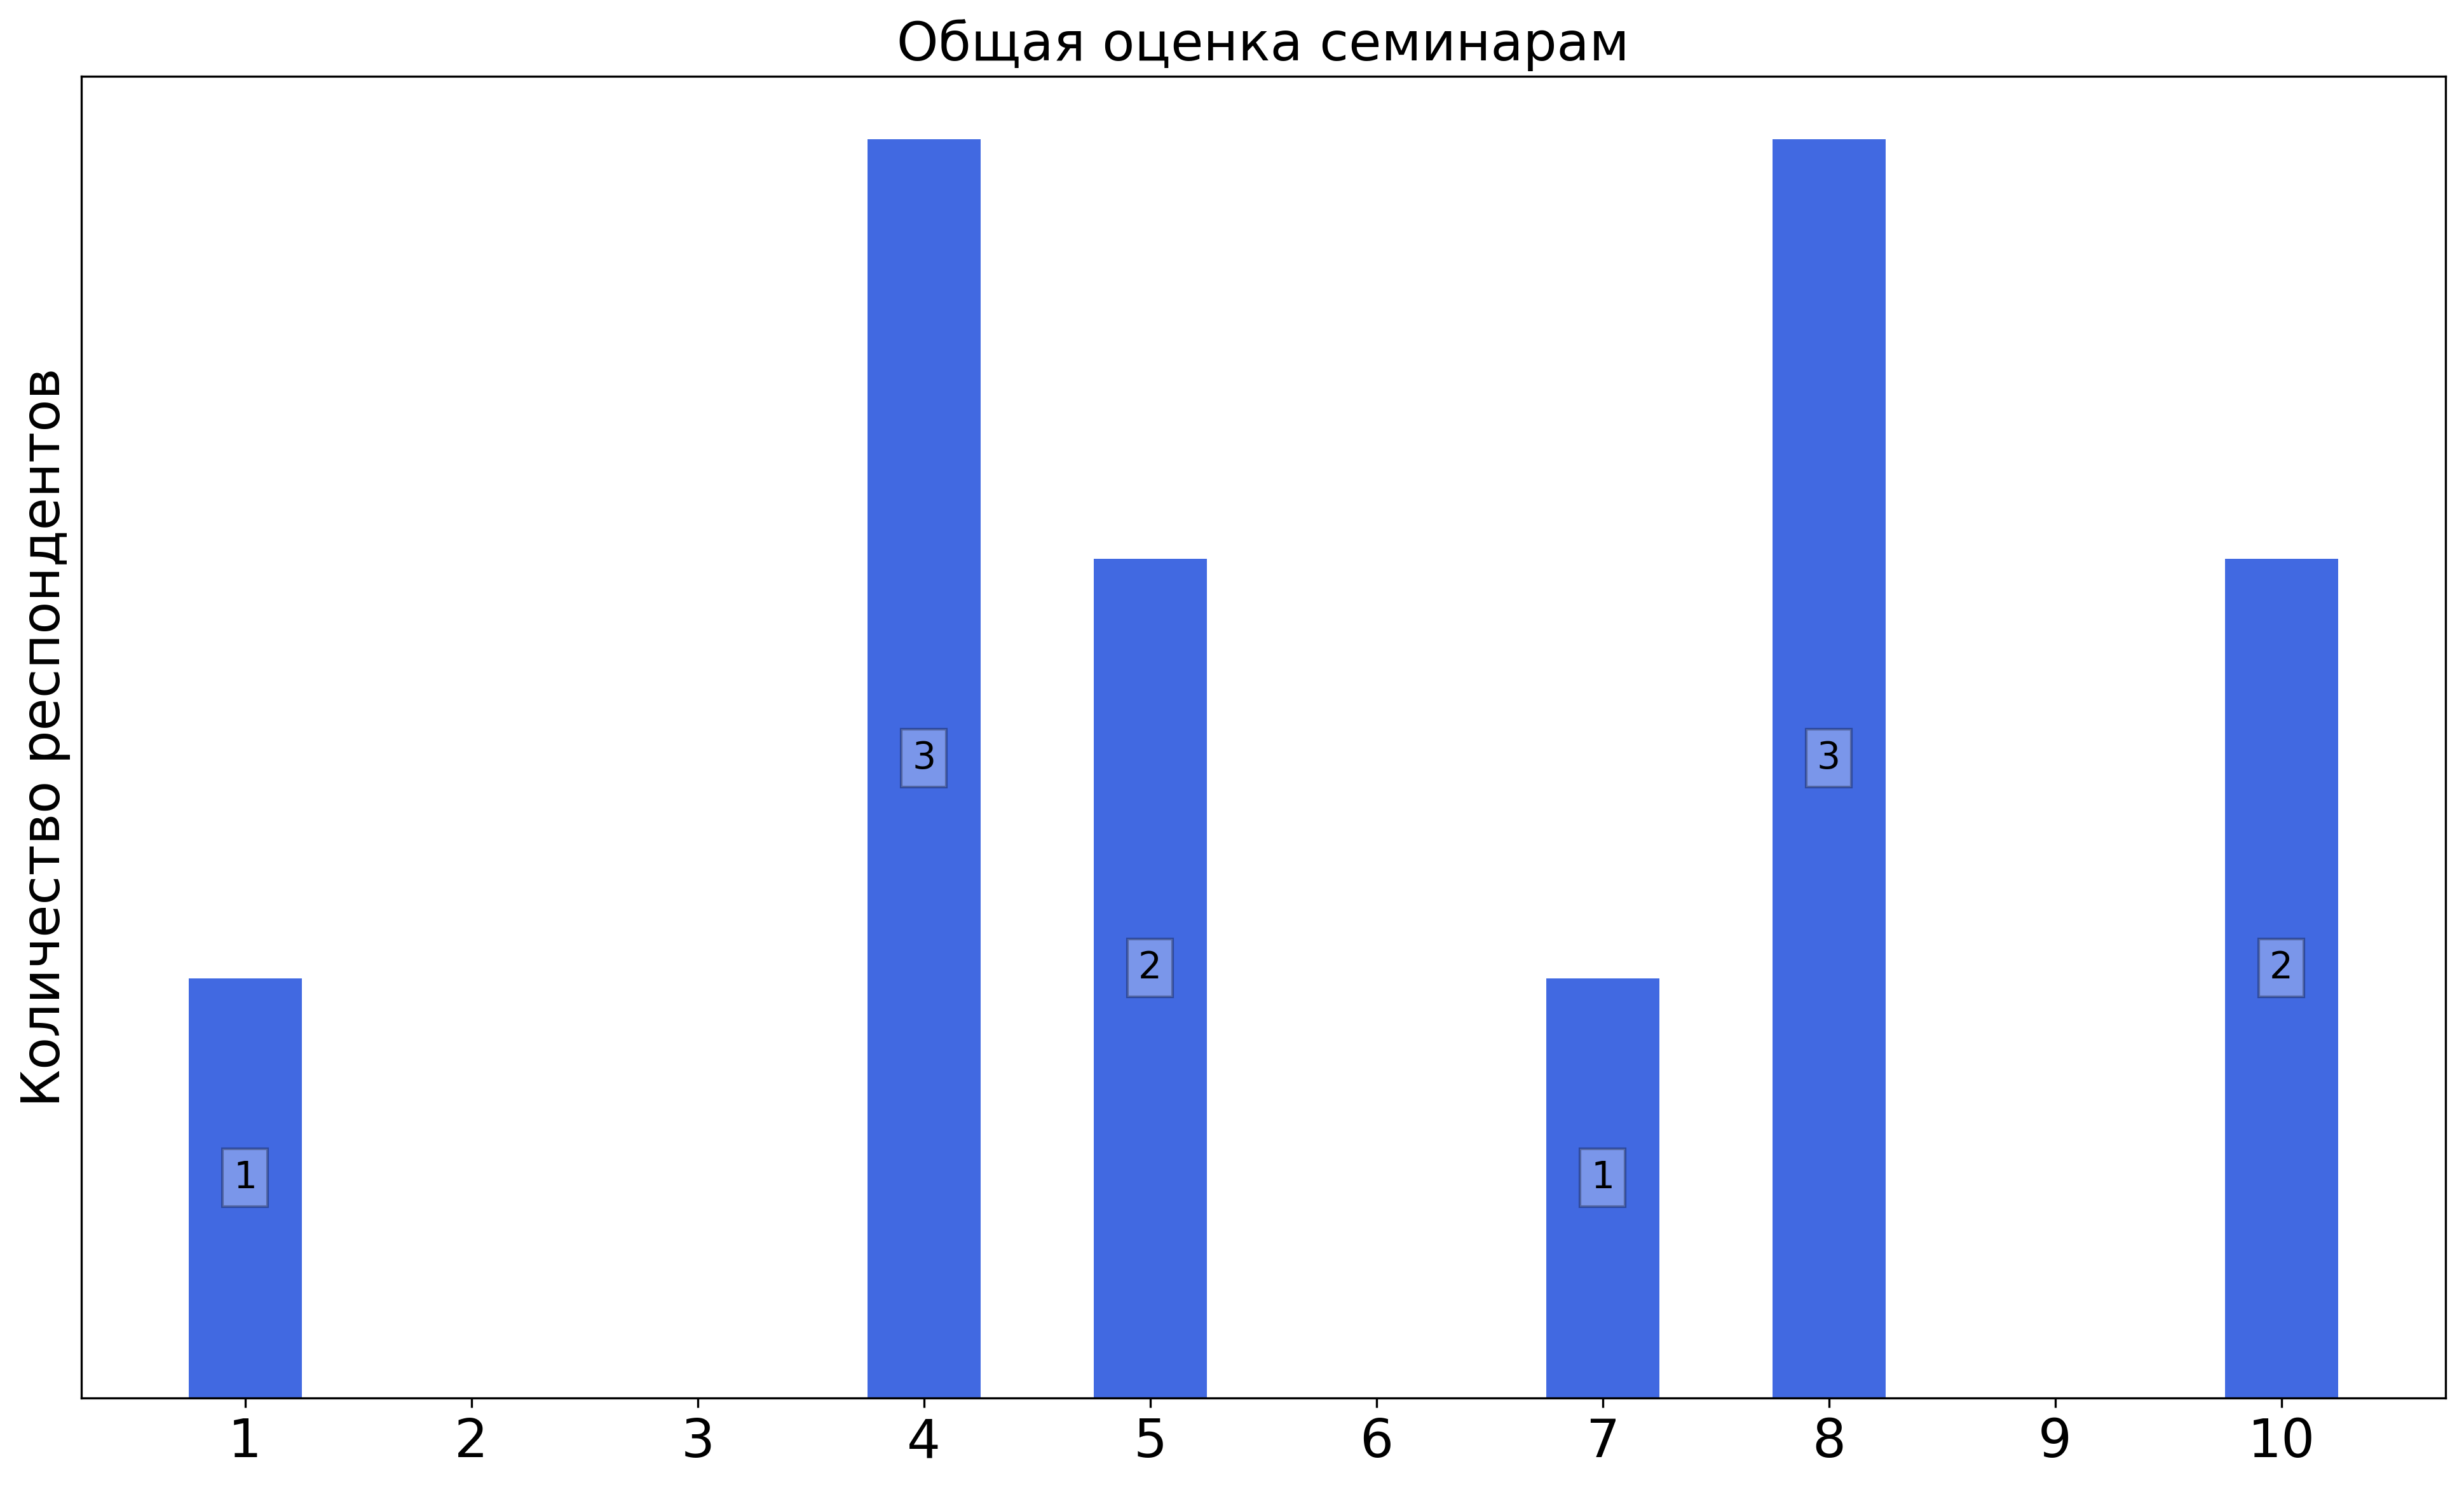
\includegraphics[width=\textwidth]{images/3 course/Теория поля/seminarists-marks-Осипов Д.Л.-3.png}
			\end{subfigure}	
			\caption{Оценки респондентов о качестве преподавания семинаров}
		\end{figure}

		\textbf{Комментарии студентов о семинаристе\protect\footnote{сохранены оригинальные орфография и пунктуация}}
            \begin{commentbox} 
                Хуже уже не будет 
            \end{commentbox} 
        
            \begin{commentbox} 
                Как преподаватель очень хорош, действительно разбирается в материале и хорошо его рассказывает. Однако отношение к студентам просто ужасное. Постоянно слышались какие-то саркастичные издевательства в духе "ну в этой аудитории, я вижу, никто ничего не понимает", прием задания осуществлялся на переменах из-за несостыковки в расписаниях. В итоге почти всей группе поставил рекомендованную уд 3 или 4 (результаты лекционных контрольных и летучек вовсе не учитывались), и экзаменаторам сказал, что мы вообще ничего весь семестр не делали. 
            \end{commentbox} 
        
            \begin{commentbox} 
                1) Сдача заданий происходила после пары и у Д.Л. не всегда было на это время. Из-за этого много задач оставалось на конец.

                2) Просто неадекватная система оценивания. В группе максимальная рекомендуемая оценка была хор7, буквально пару хоров, остальные уды.

                3) Из приятного отличное объяснение задач.  
            \end{commentbox} 
        
            \begin{commentbox} 
                Почти всей группе поставил уды, даже самым умным, не учитывает кр лектора 
            \end{commentbox} 
        
            \begin{commentbox} 
                Человек с очень странными представлениями о мире. Очень любит начать рассказывать про: Древние Арабские цивилизации, Ложность почти всех современных научных представлений о мире, Отсутвие у Земли твердого ядра - магнитное поле объясняет наличием небарионной материи в центре Земли, Теория струн, Глупость всех астрономов, Глупость студентов. Из веселых вещей - провел тест на одном из семинаров, на следующем оказалось, что результаты теста он потерял, поэтому провел тест еще раз. Естественно люди к этому были не готовы, а кто-то и вовсе опоздал и не успел написать (переписывать не разрешается) 
            \end{commentbox} 
        
            \begin{commentbox} 
                Было бы всё идеально, если бы не система оценивания. В конце вся группа получила уд 3 или уд 4, за исключением 2 человек.(отла ни у кого)  
            \end{commentbox} 
        
            \begin{commentbox} 
                Неординарный преподаватель. Сдавали ему задачи каждую неделю в течение семестра, знания получили. 
            \end{commentbox} 
        
            \begin{commentbox} 
                Хорошо объясняет, доходчиво. Не терпит глупых вопросов по типу 'я прослушал'. Требовал сдавать задачи по одной, что занимало время, а на физтехе он 1 день в неделю. 
            \end{commentbox} 


    \subsubsection{Отзыв студентов о семинарах. Семинарист: Толоконников С.В.}
        \begin{figure}[H]
            \centering
            \begin{subfigure}[b]{0.45\textwidth}
                \centering
                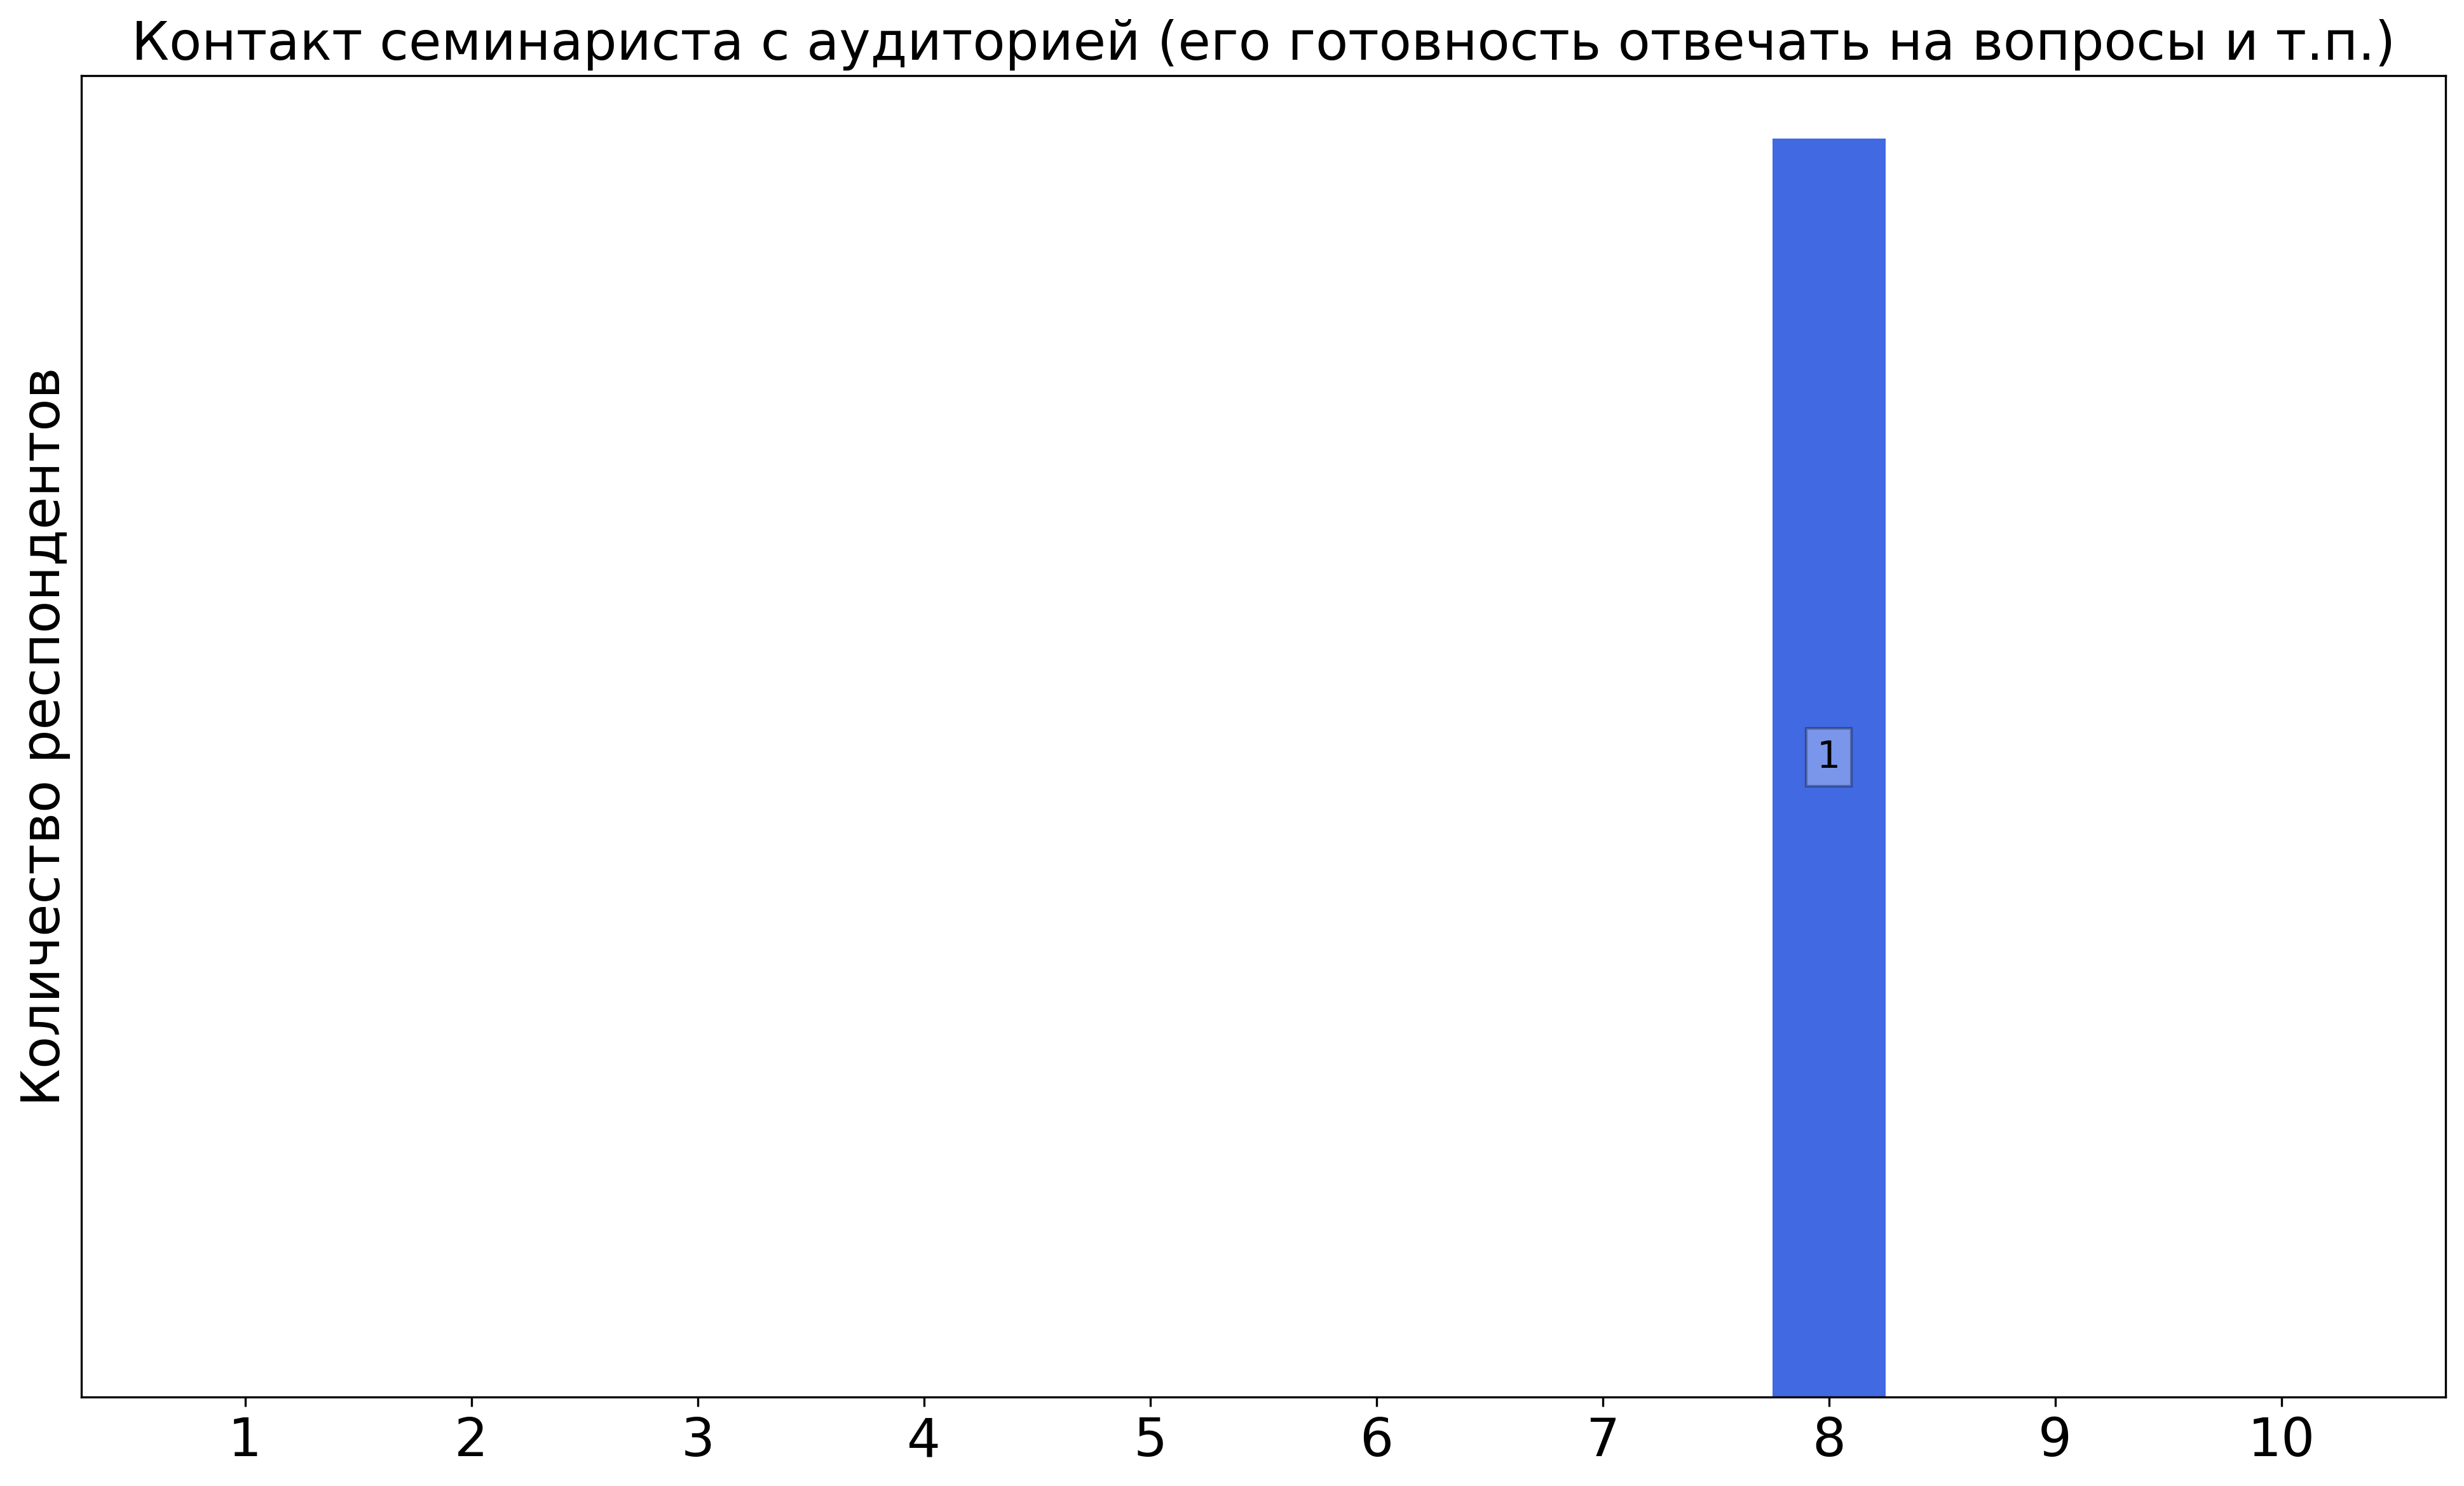
\includegraphics[width=\textwidth]{images/3 course/Теория поля/seminarists-marks-Толоконников С.В.-0.png}
            \end{subfigure}
            \begin{subfigure}[b]{0.45\textwidth}
                \centering
                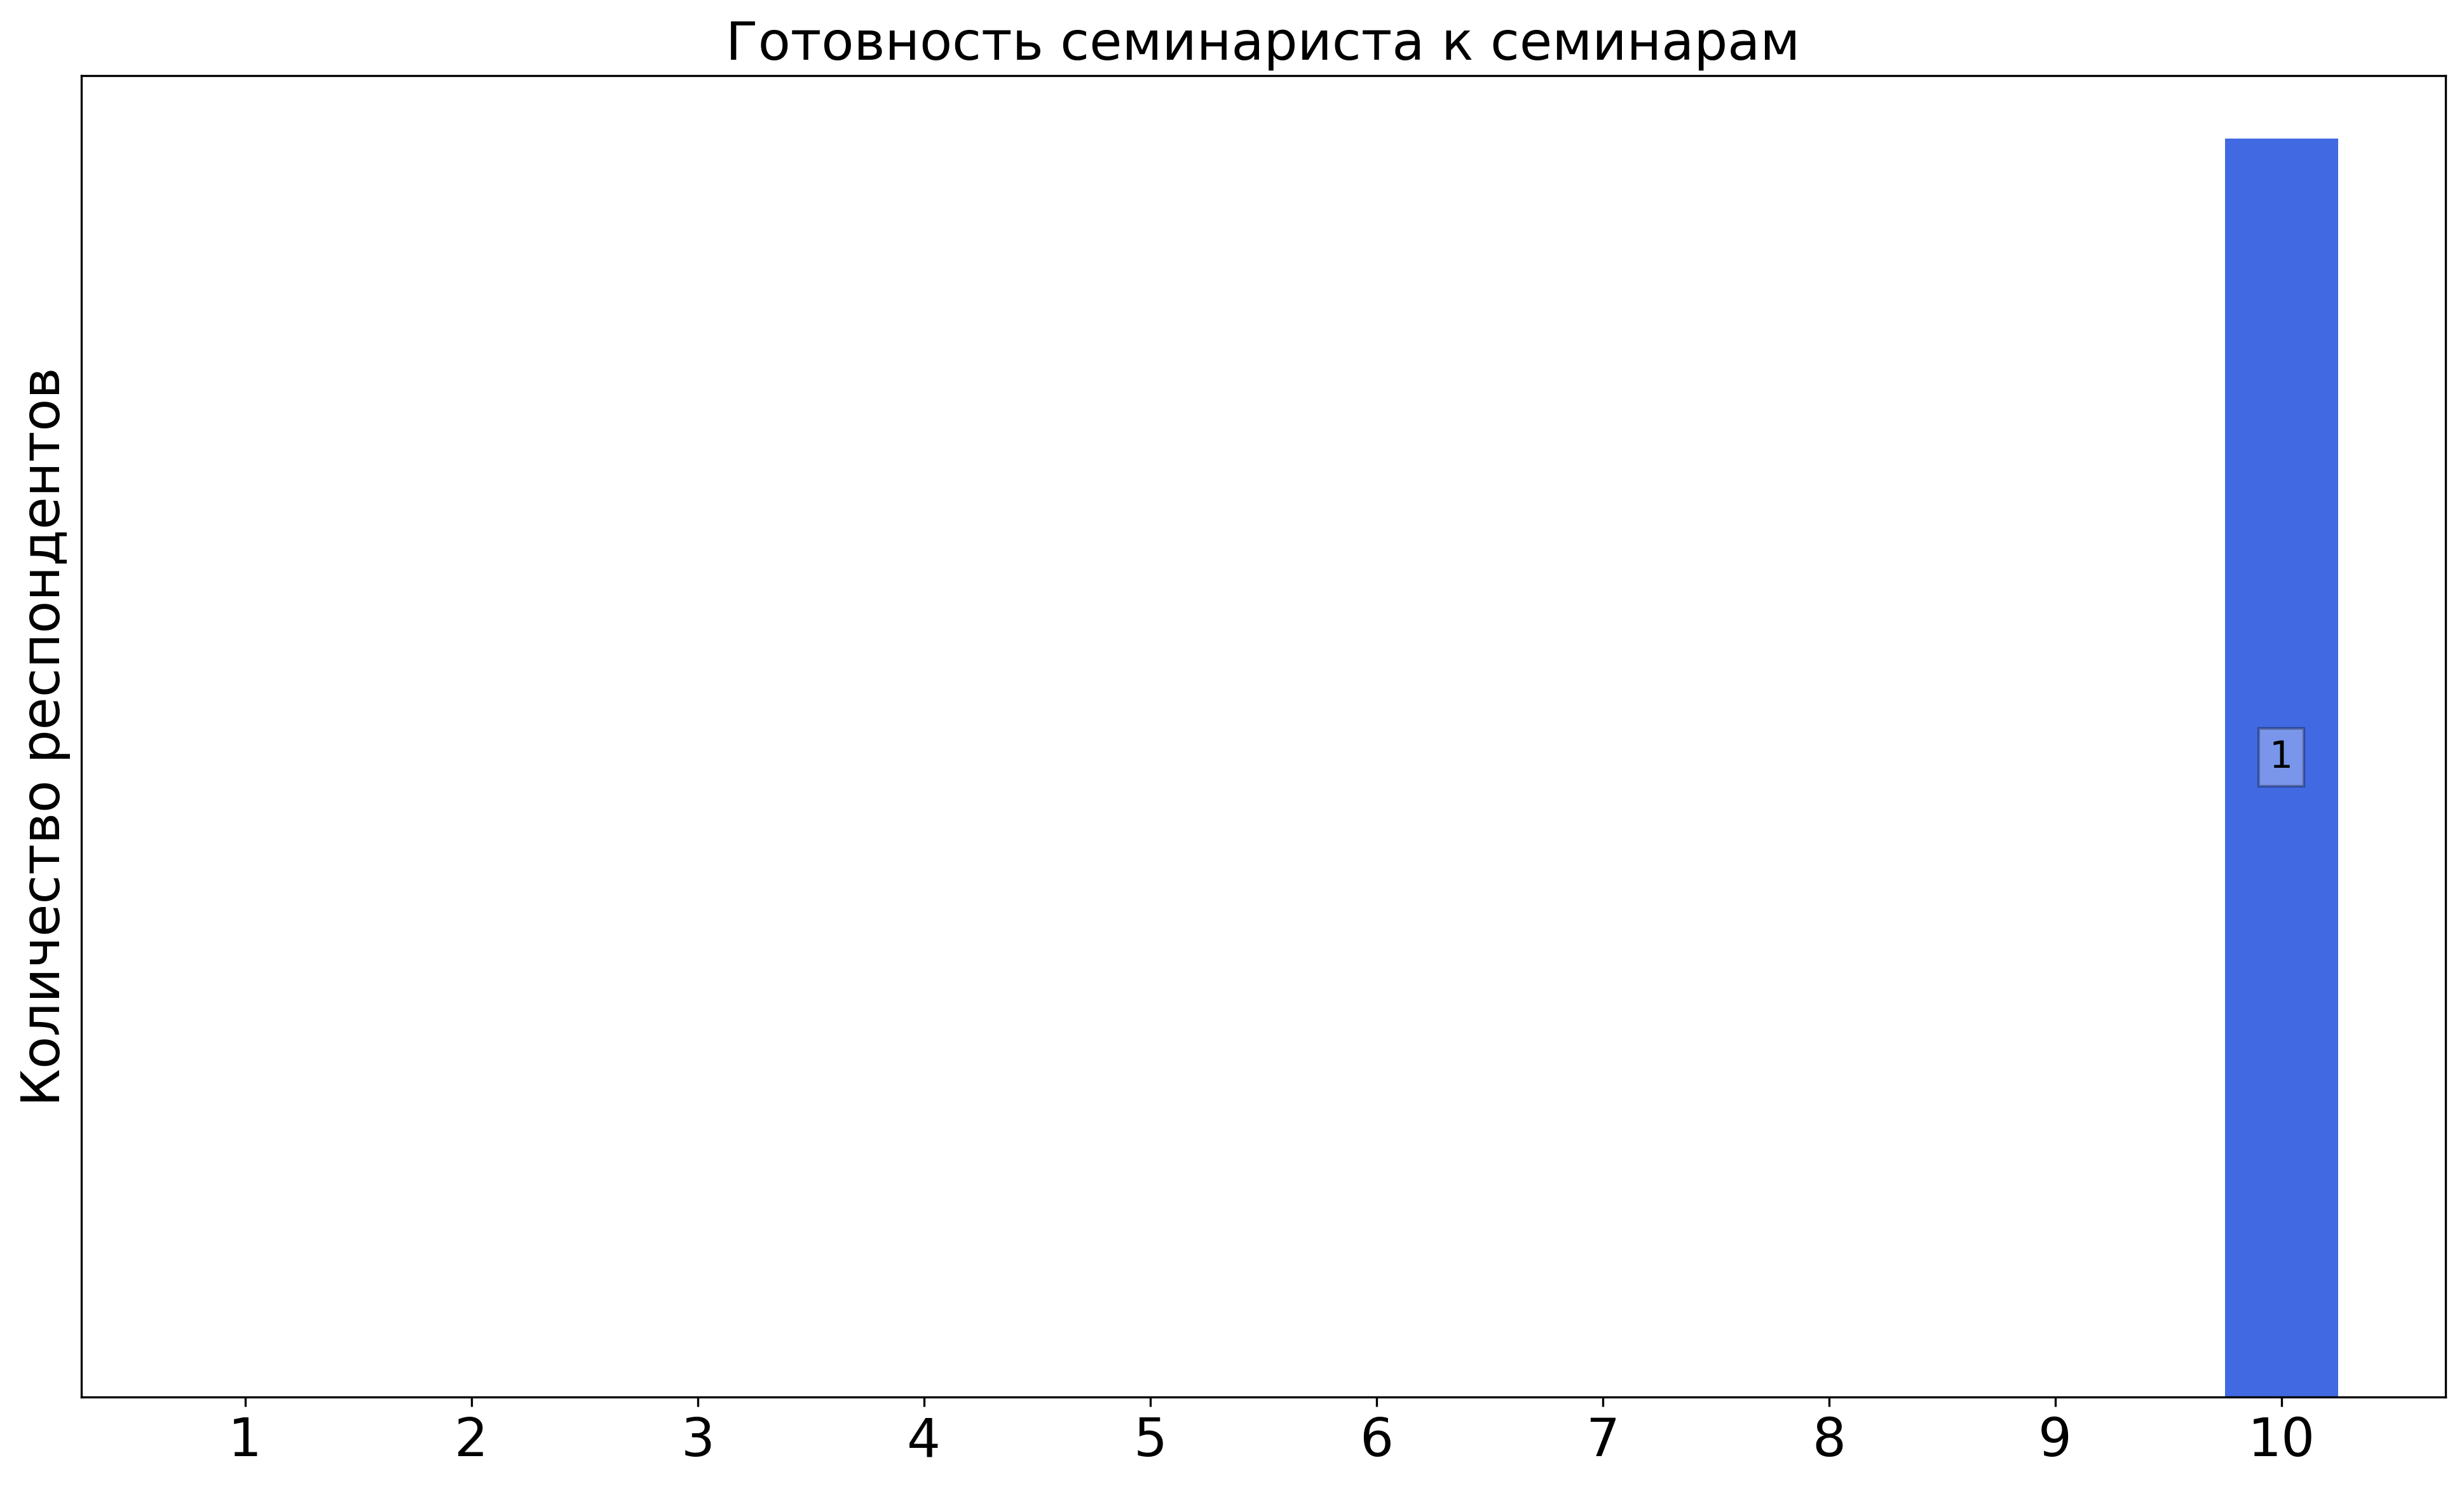
\includegraphics[width=\textwidth]{images/3 course/Теория поля/seminarists-marks-Толоконников С.В.-1.png}
            \end{subfigure}
            \begin{subfigure}[b]{0.45\textwidth}
                \centering
                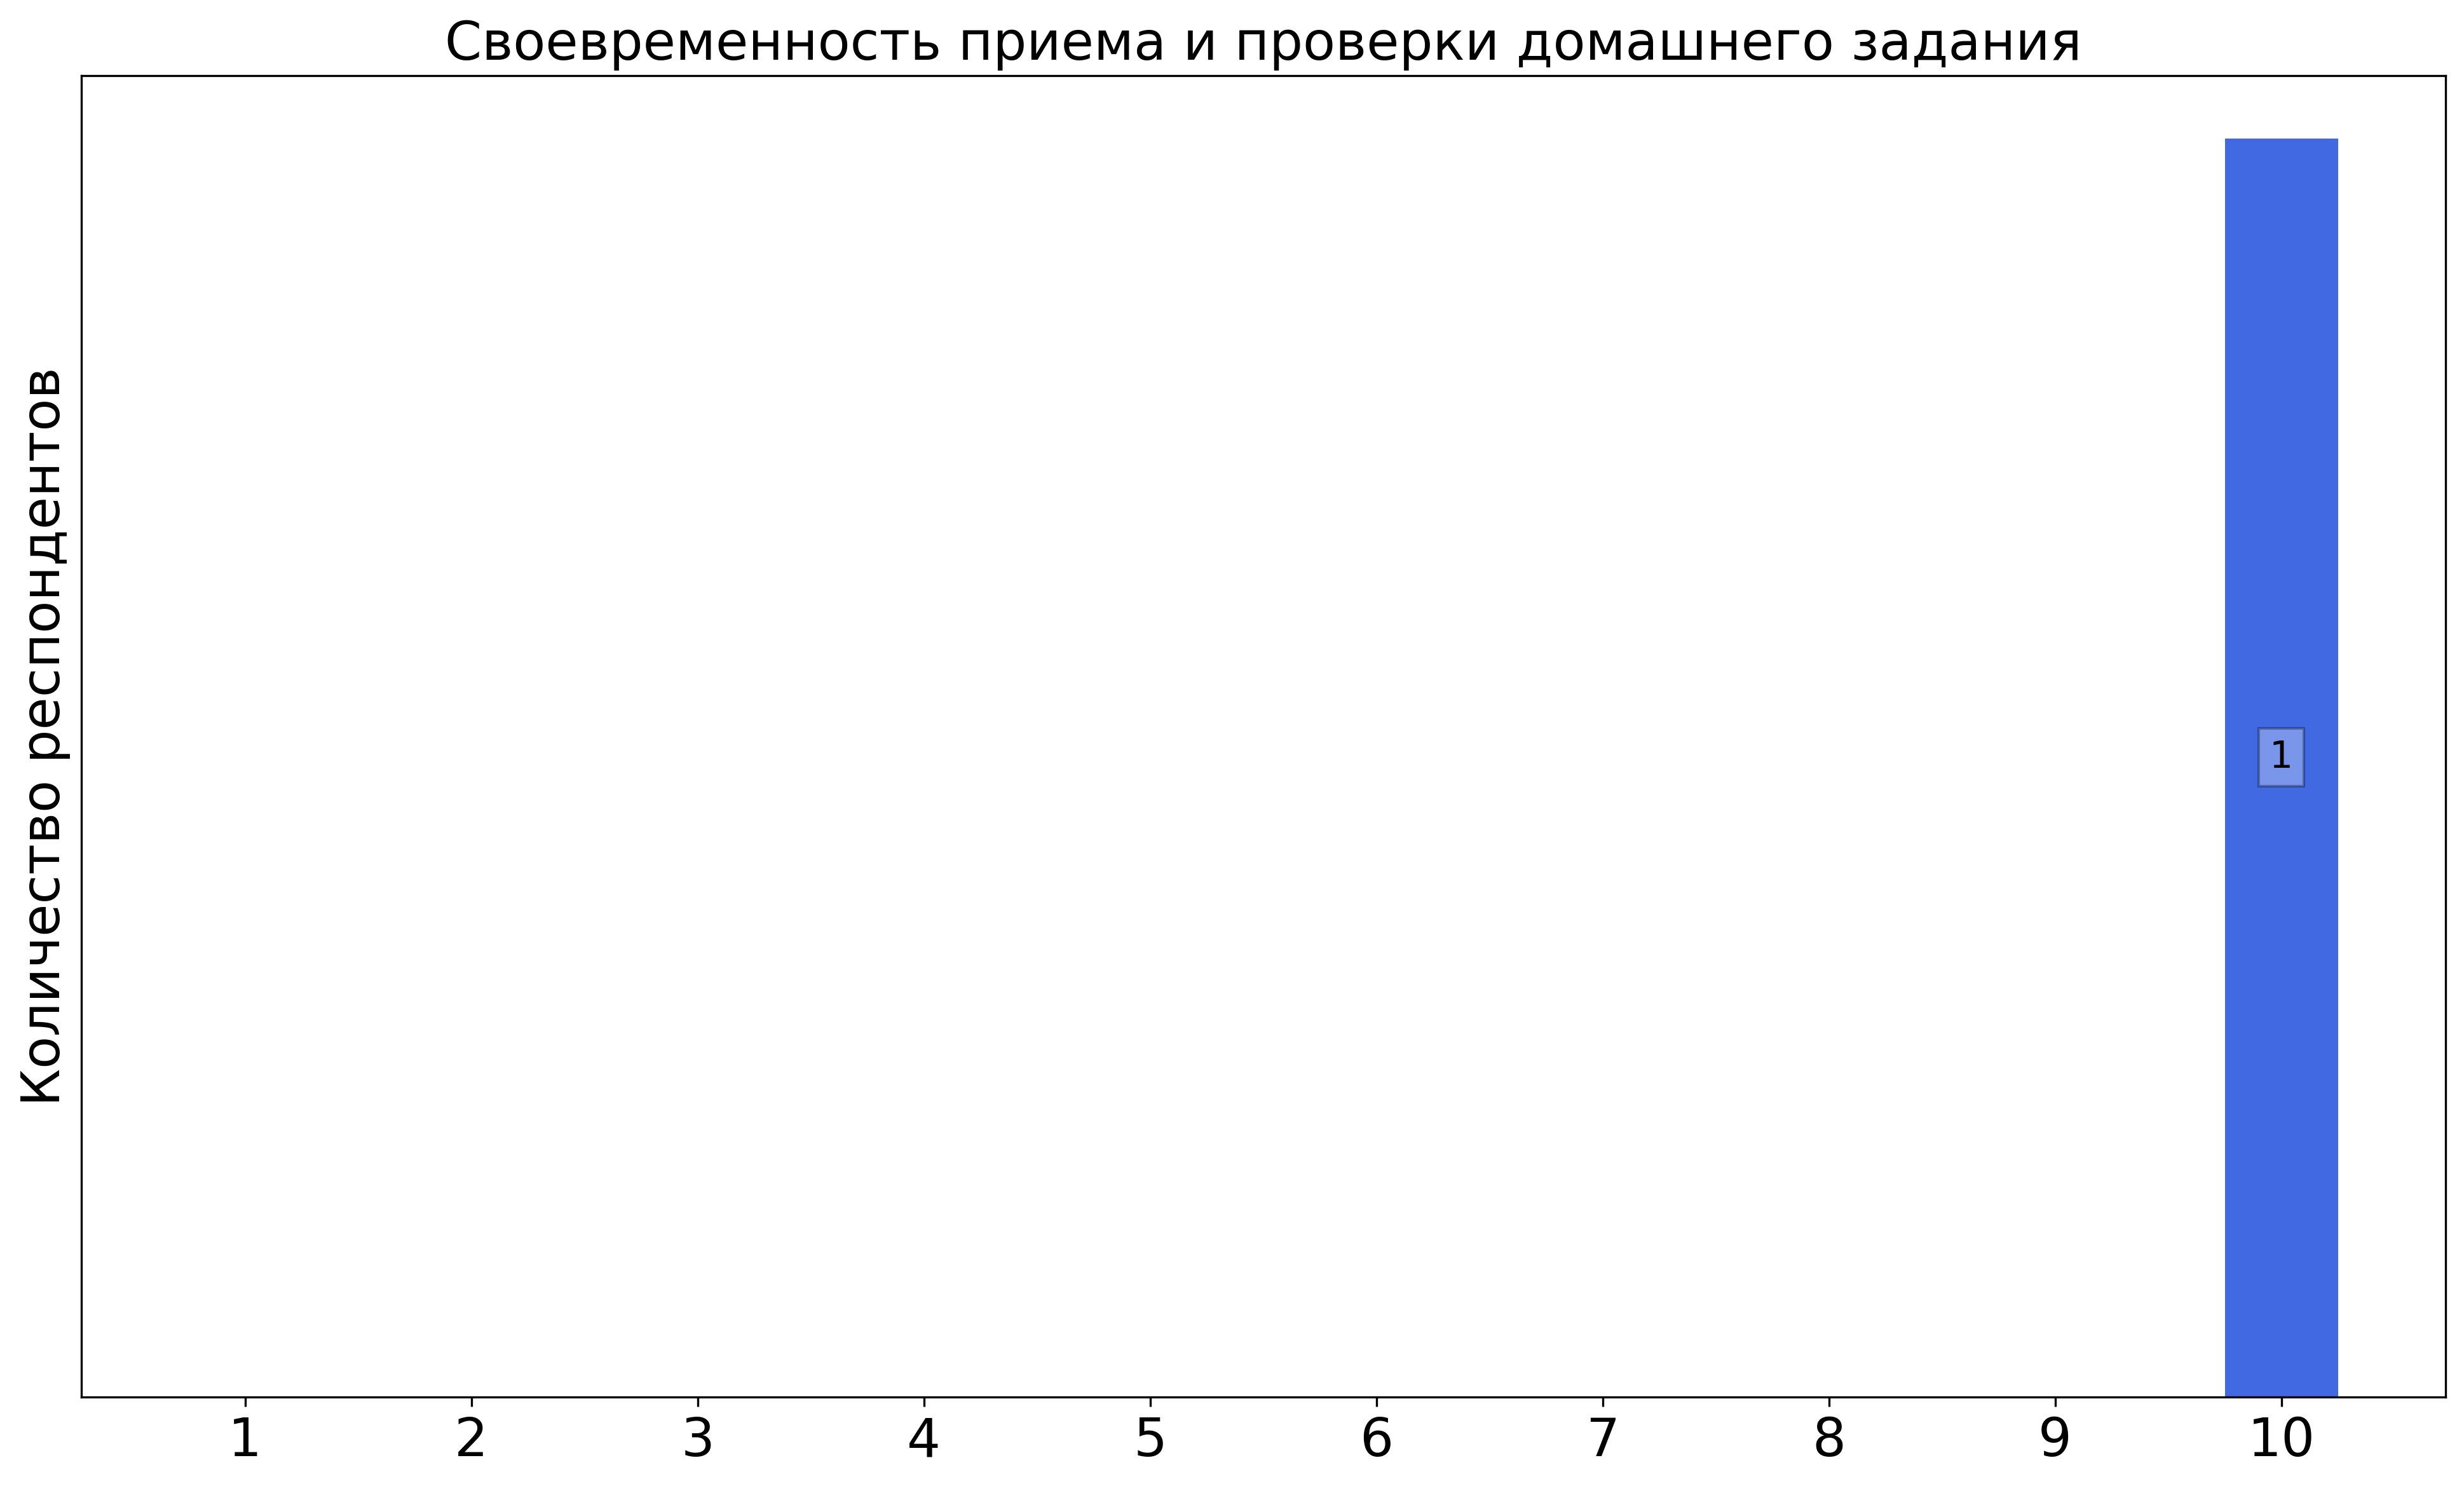
\includegraphics[width=\textwidth]{images/3 course/Теория поля/seminarists-marks-Толоконников С.В.-2.png}
            \end{subfigure}
            \begin{subfigure}[b]{0.45\textwidth}
                \centering
                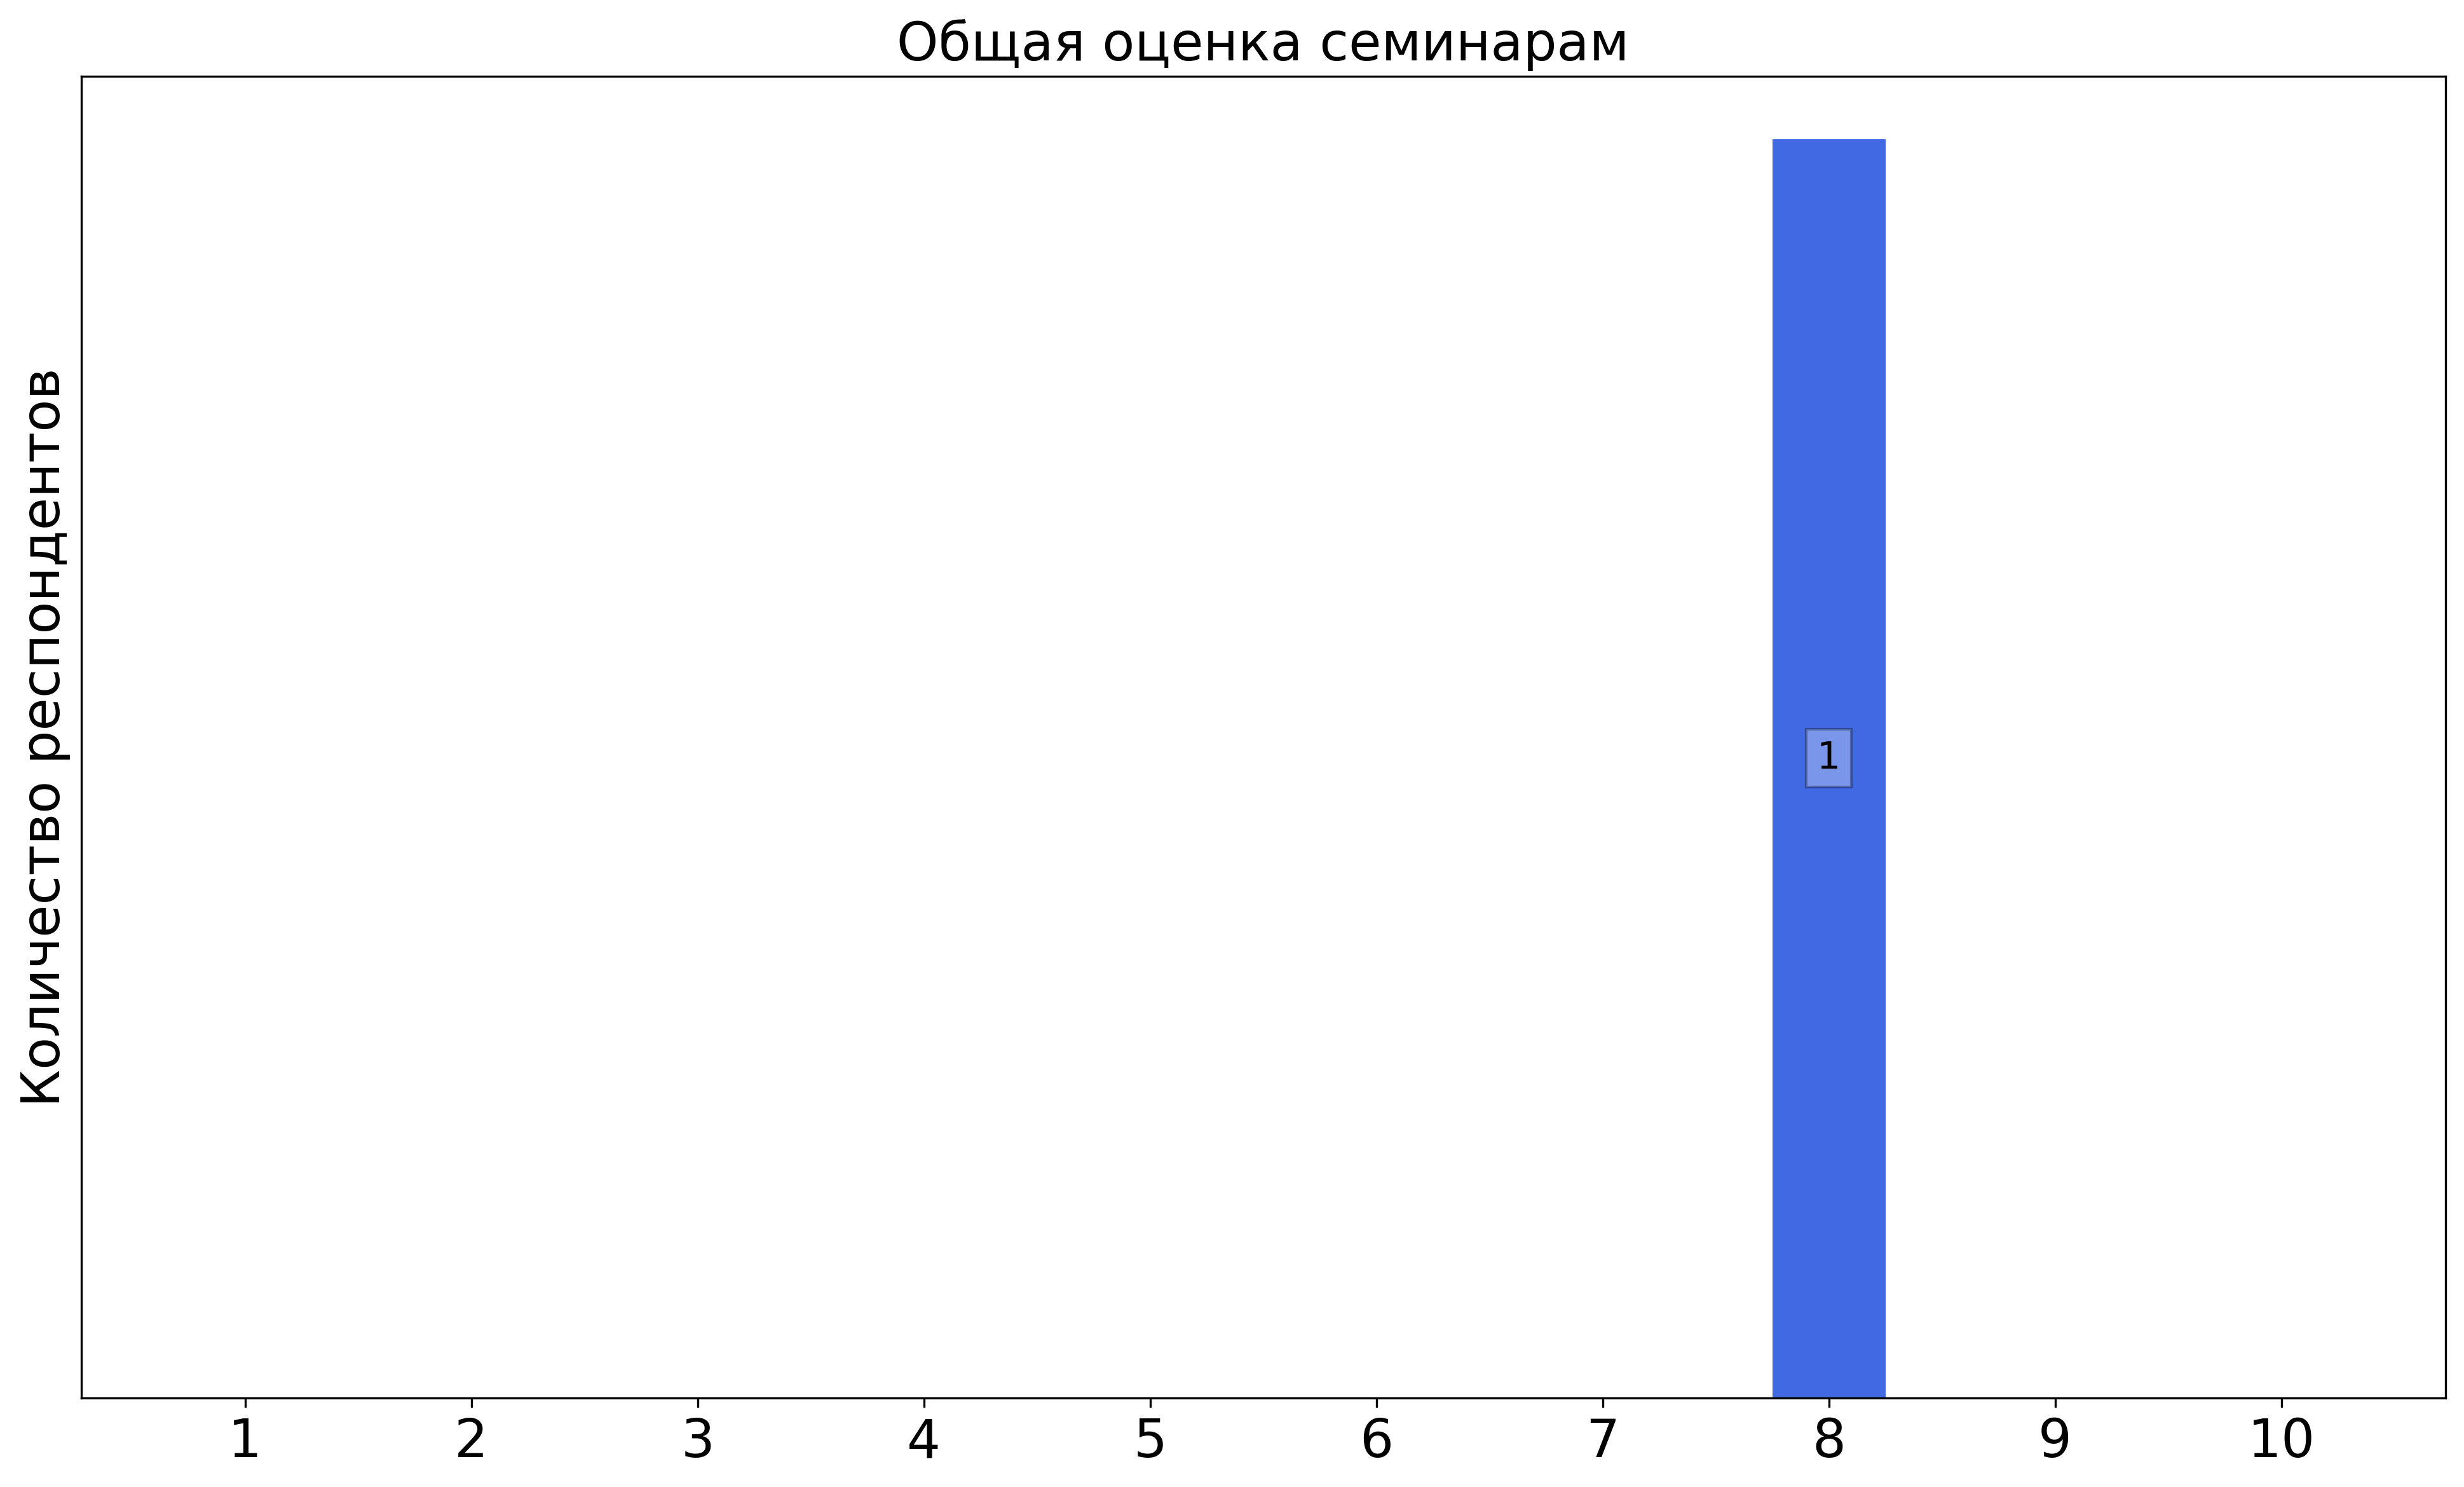
\includegraphics[width=\textwidth]{images/3 course/Теория поля/seminarists-marks-Толоконников С.В.-3.png}
            \end{subfigure}	
            \caption{Оценки респондентов о качестве преподавания семинаров}
        \end{figure}

        
    \subsubsection{Отзыв студентов о семинарах. Семинарист: Фомичев С.В.}
		\begin{figure}[H]
			\centering
			\begin{subfigure}[b]{0.45\textwidth}
				\centering
				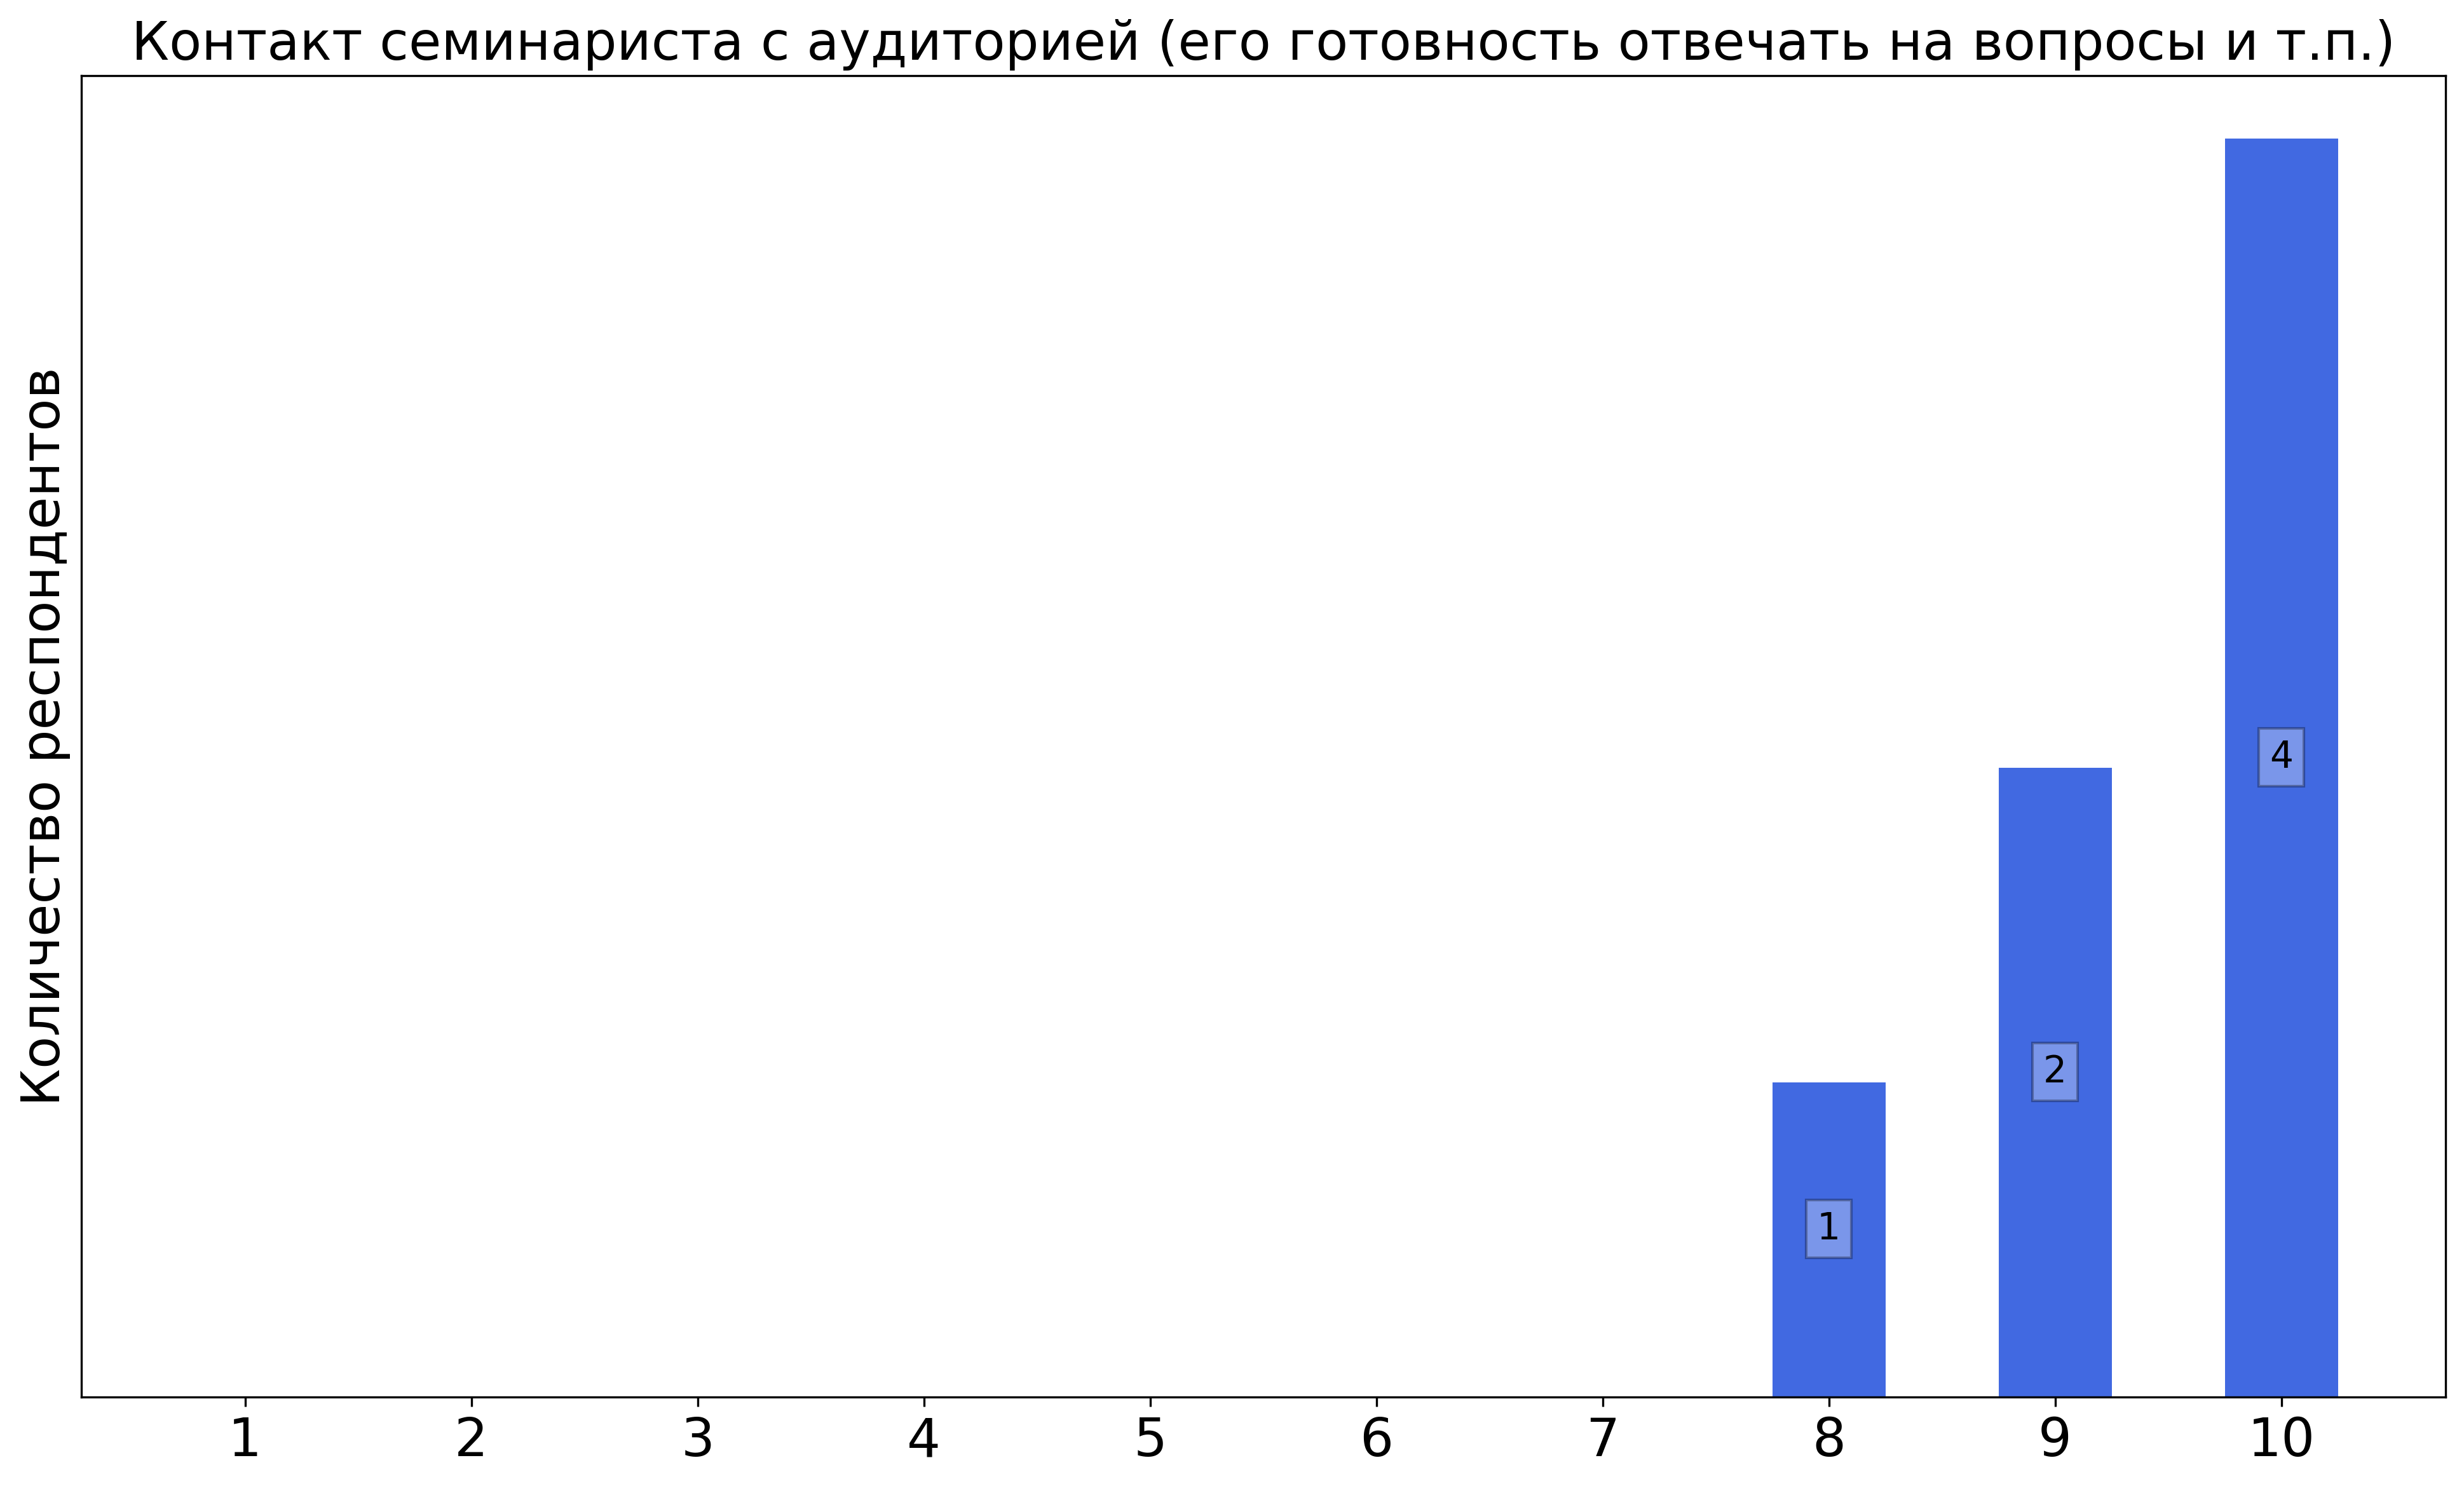
\includegraphics[width=\textwidth]{images/3 course/Теория поля/seminarists-marks-Фомичев С.В.-0.png}
			\end{subfigure}
			\begin{subfigure}[b]{0.45\textwidth}
				\centering
				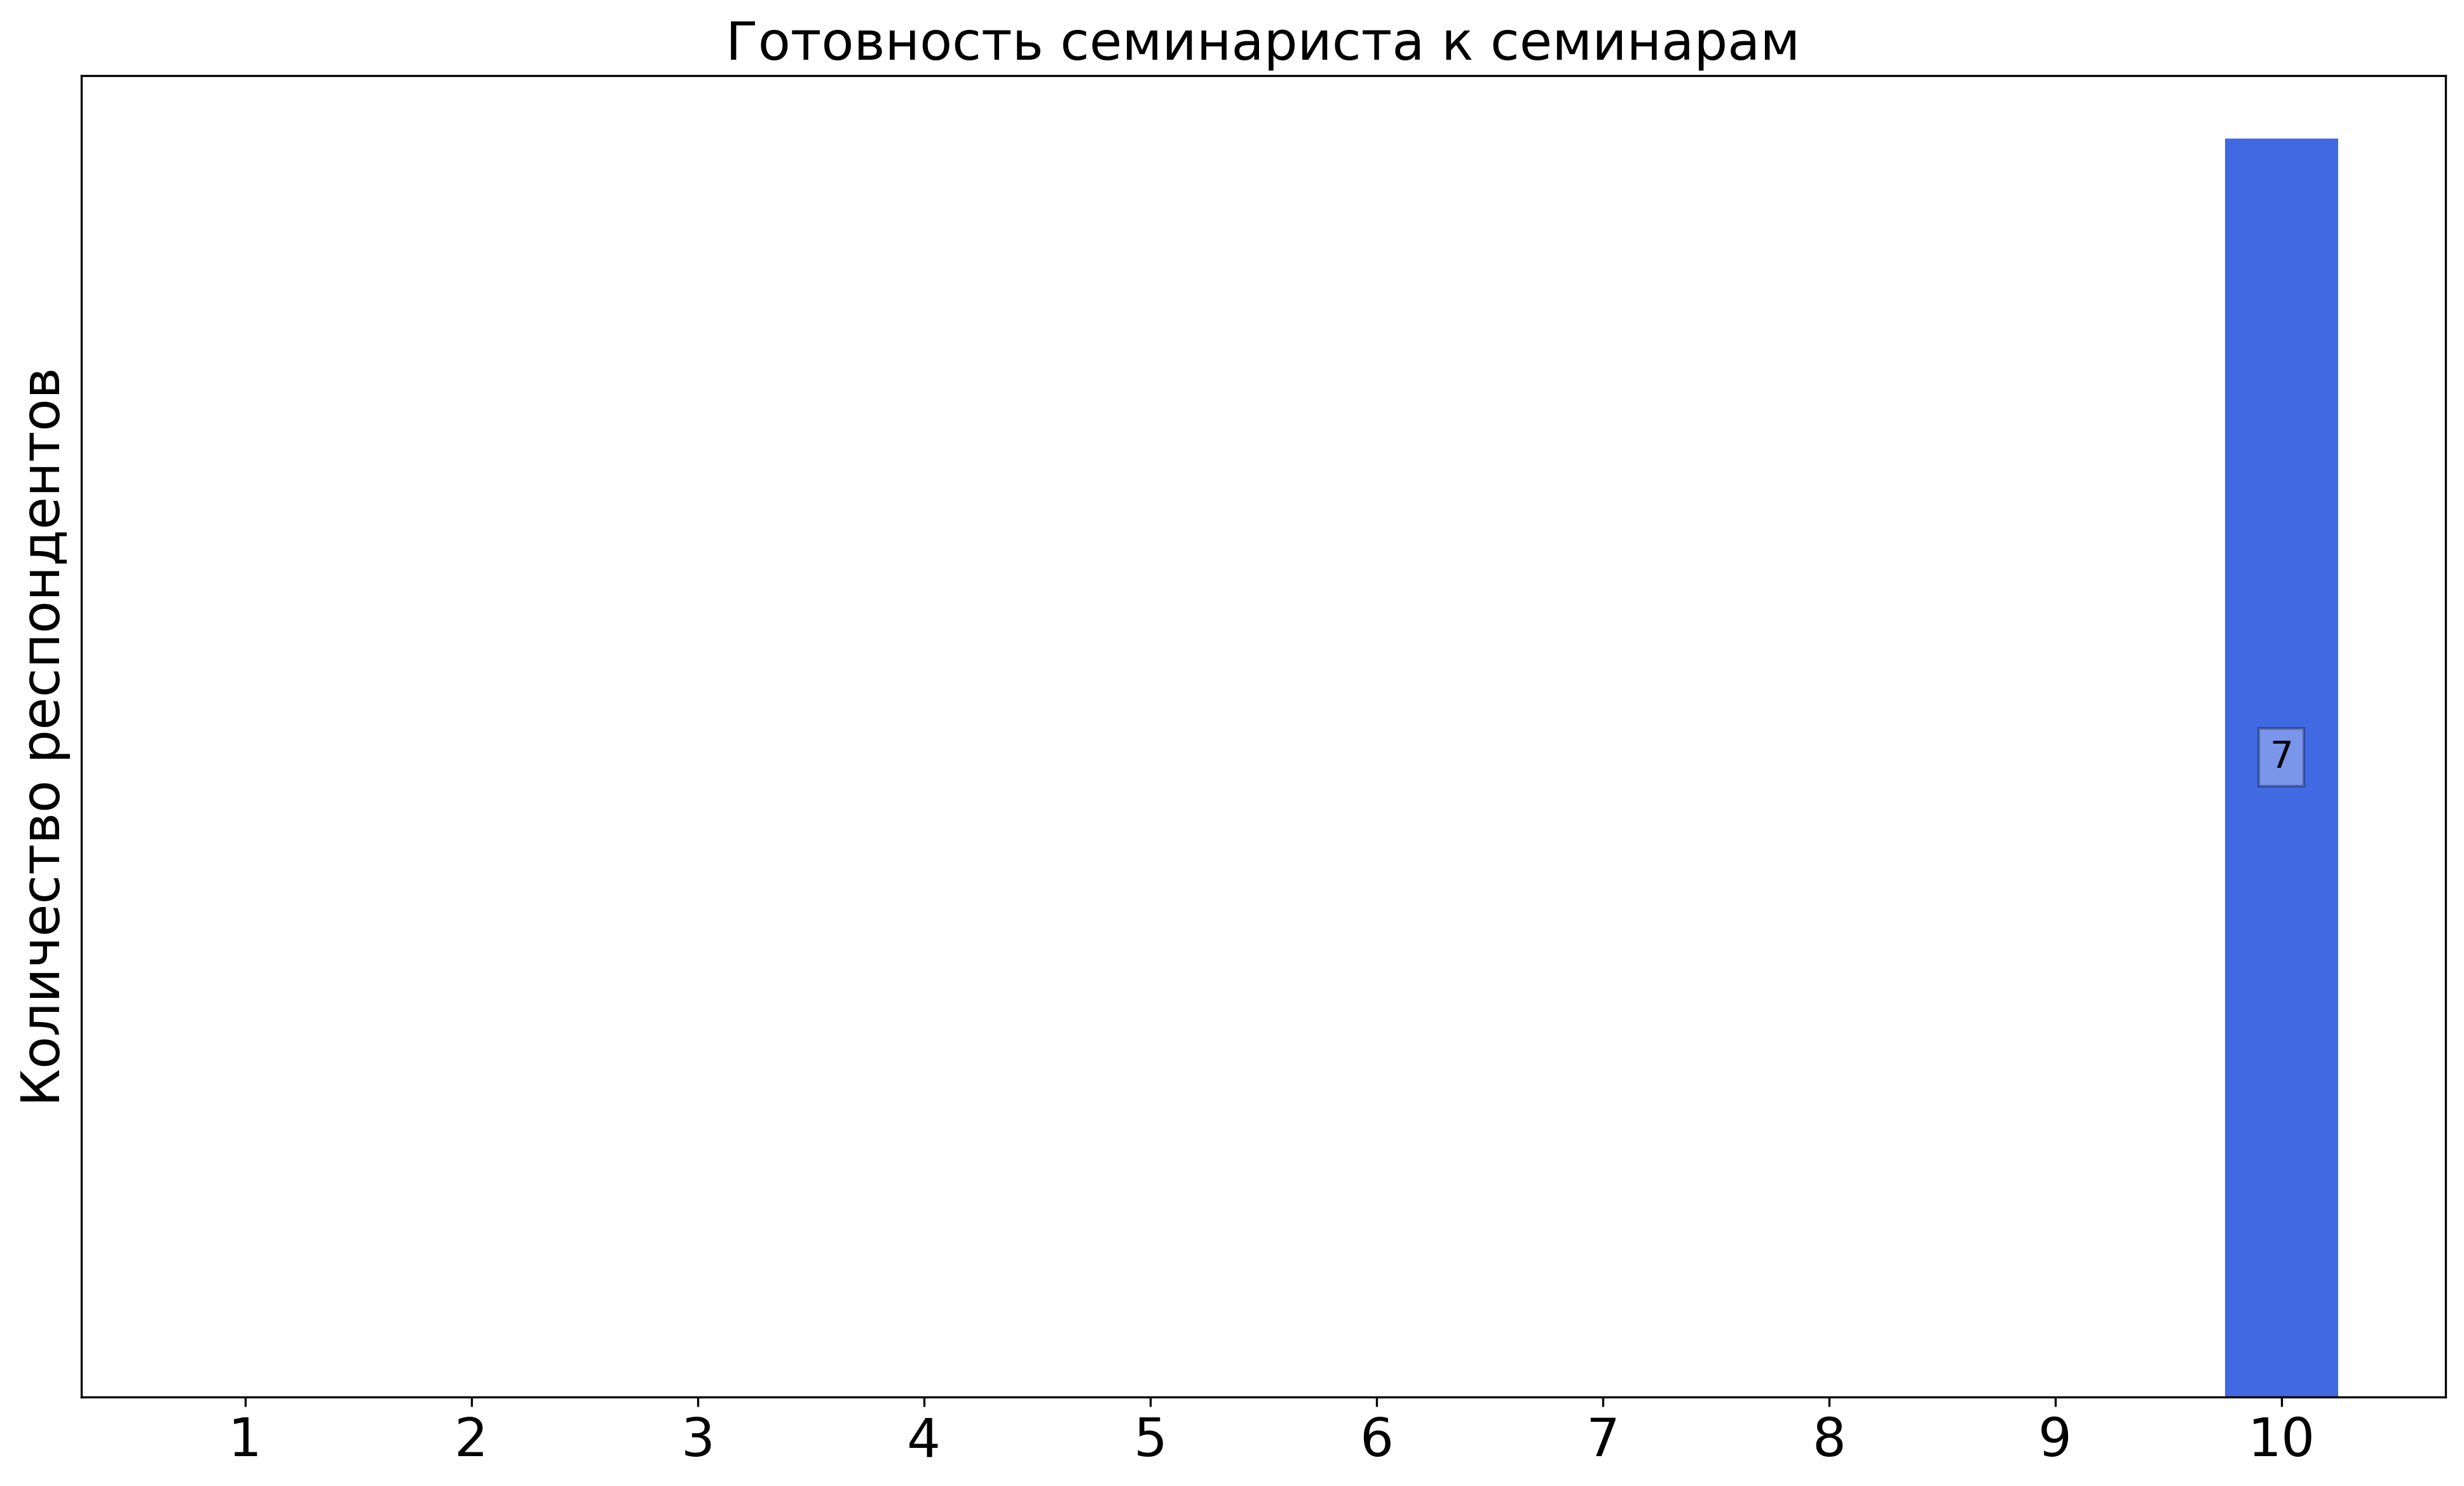
\includegraphics[width=\textwidth]{images/3 course/Теория поля/seminarists-marks-Фомичев С.В.-1.png}
			\end{subfigure}
			\begin{subfigure}[b]{0.45\textwidth}
				\centering
				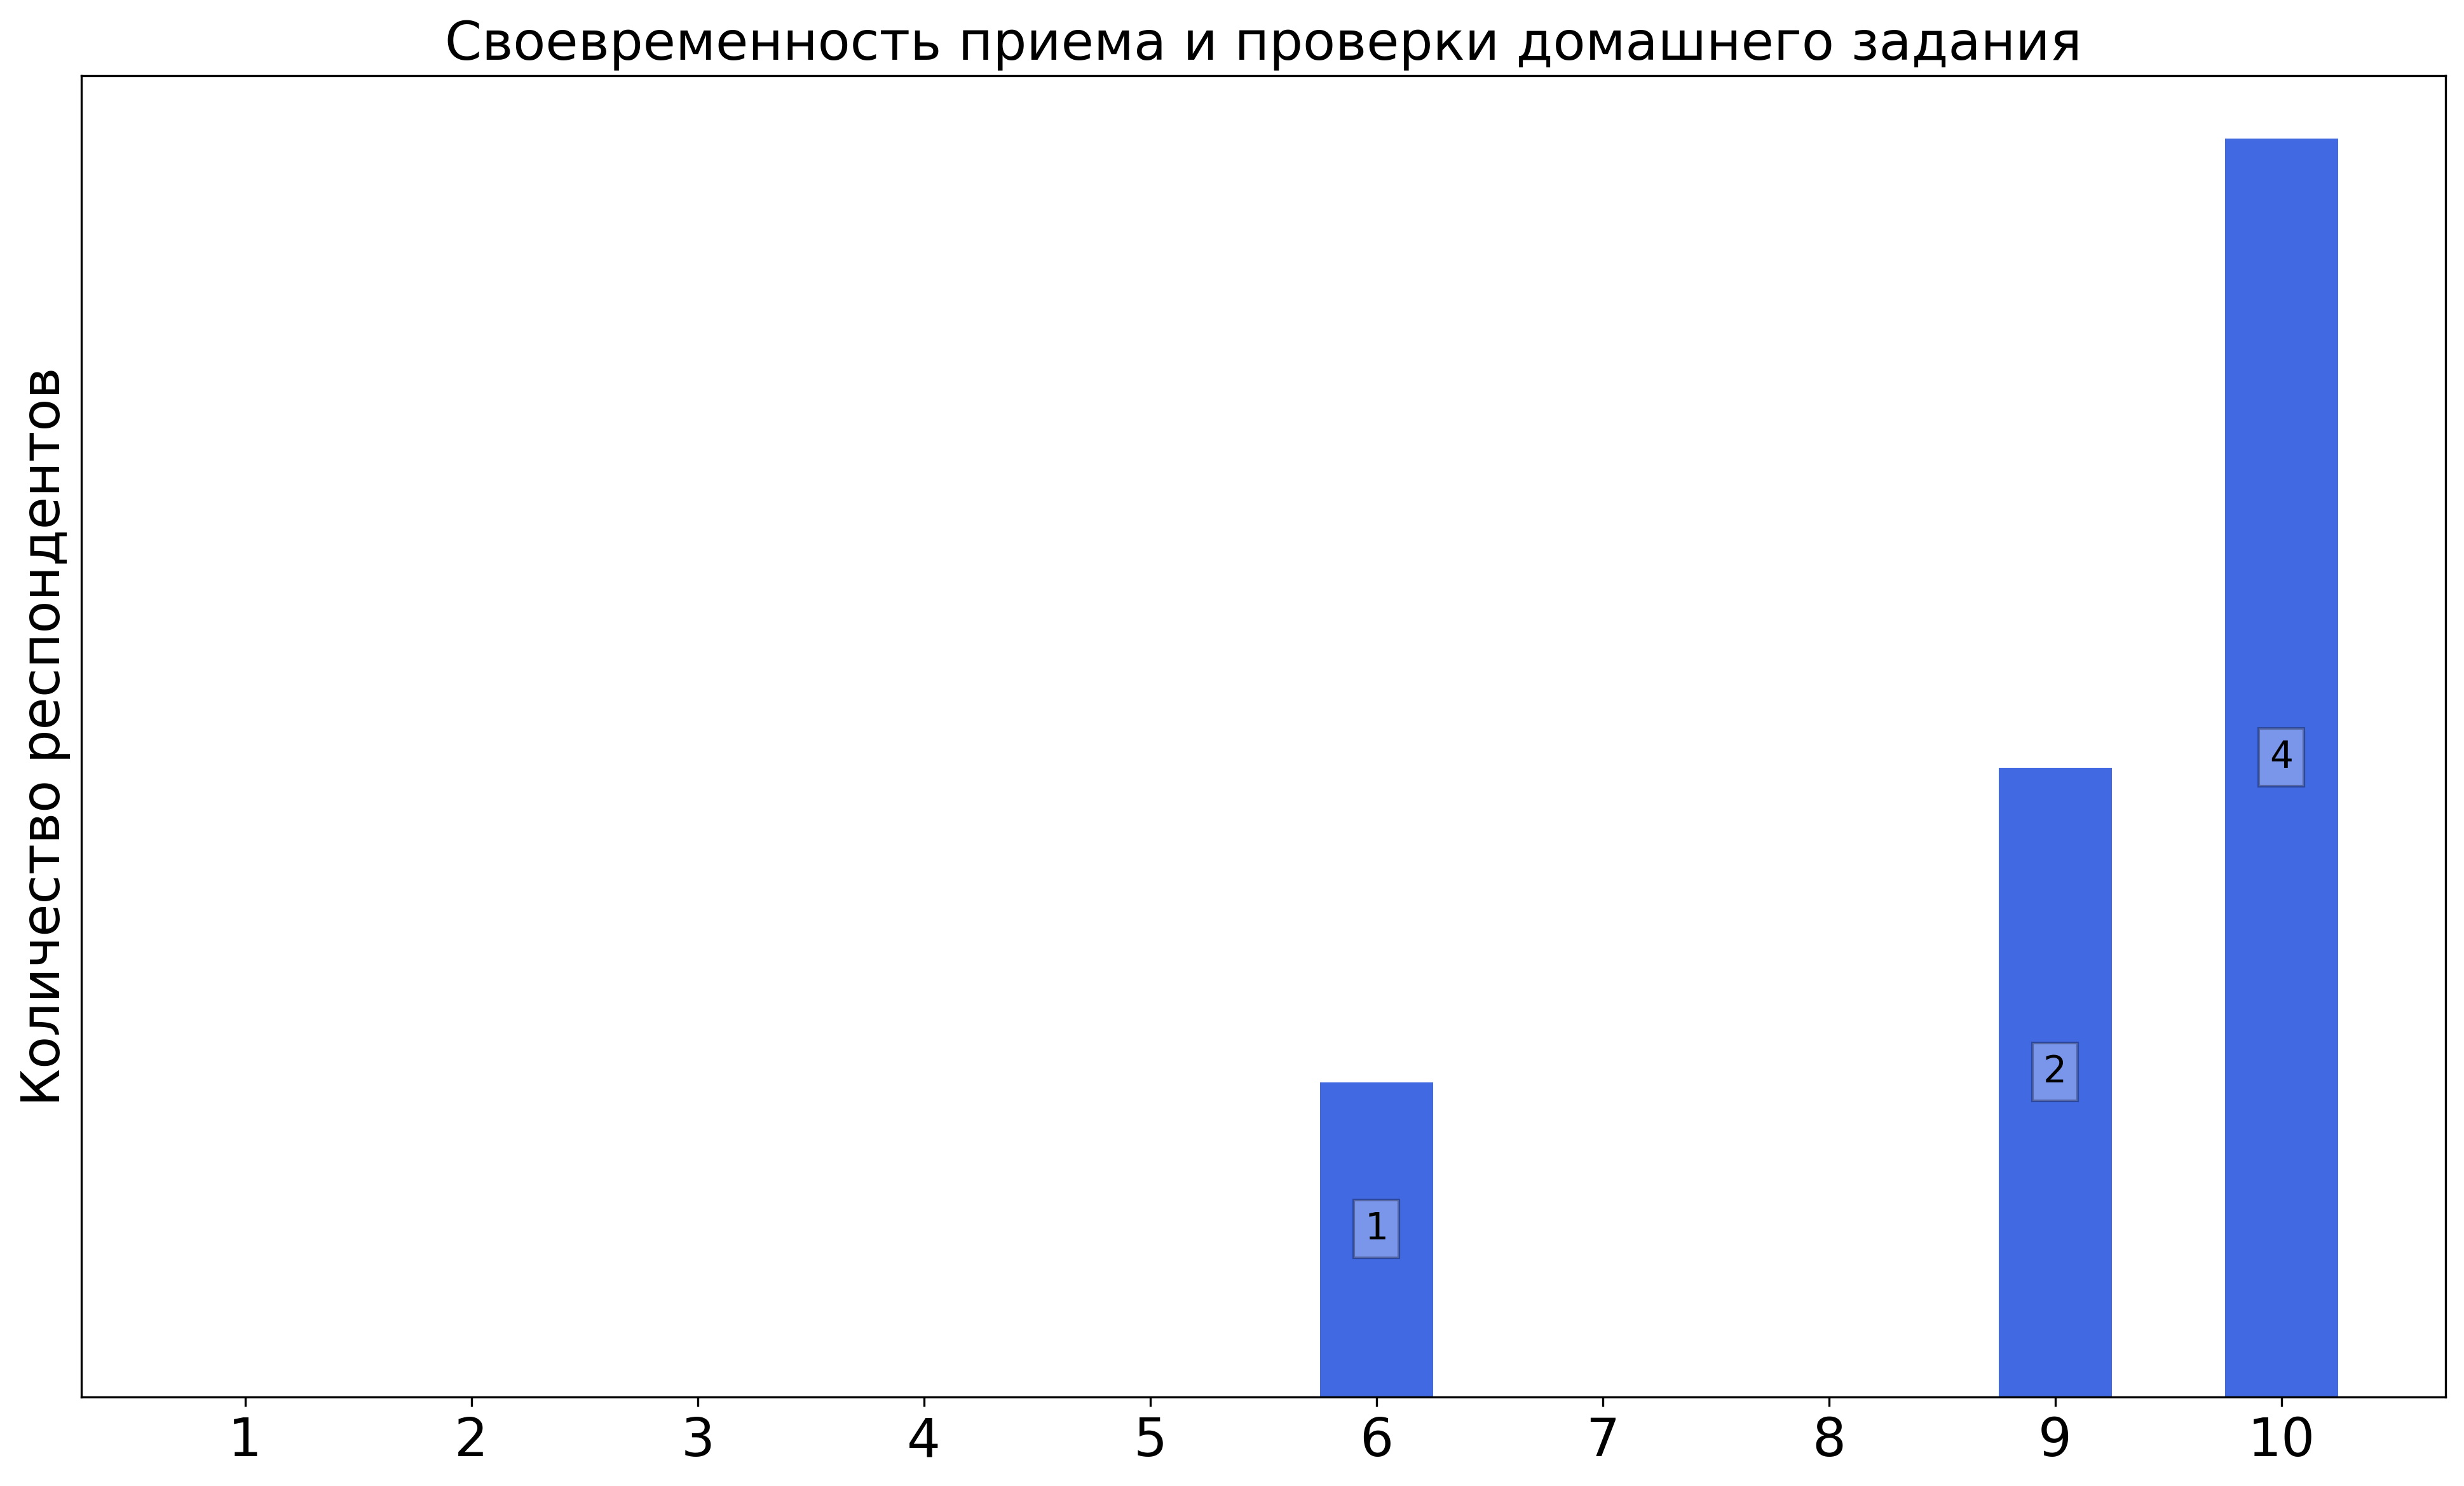
\includegraphics[width=\textwidth]{images/3 course/Теория поля/seminarists-marks-Фомичев С.В.-2.png}
			\end{subfigure}
			\begin{subfigure}[b]{0.45\textwidth}
				\centering
				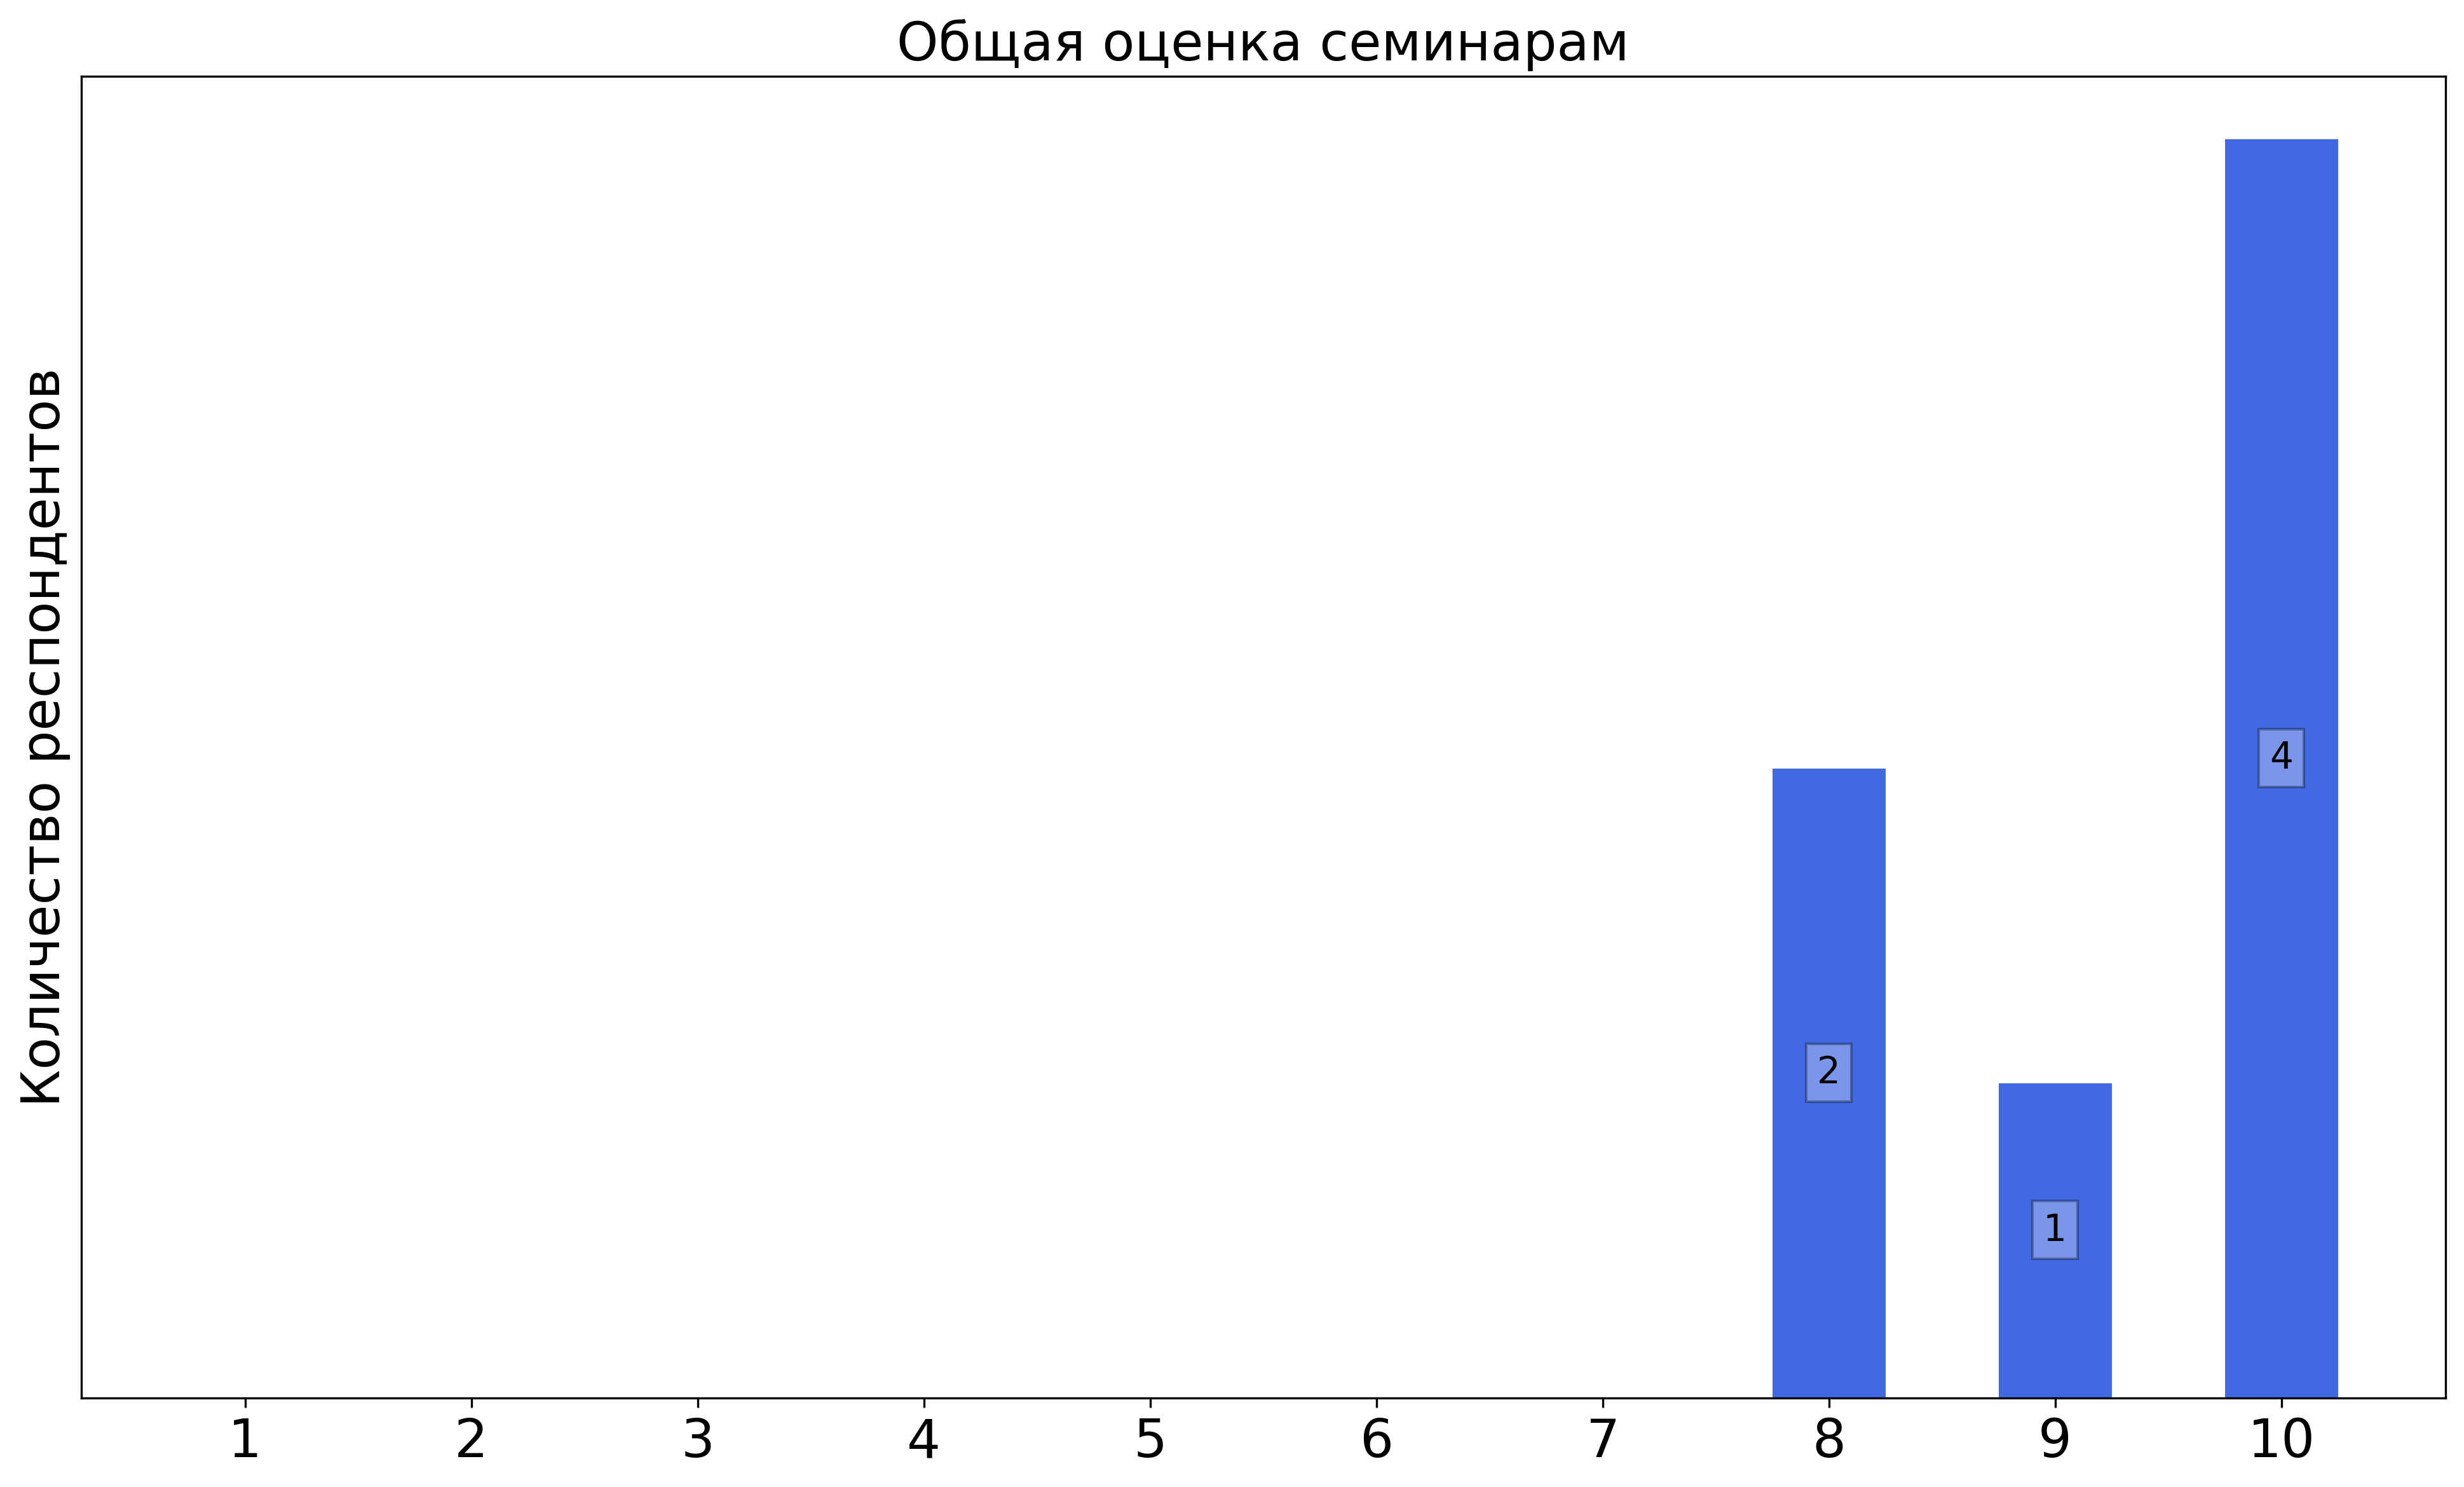
\includegraphics[width=\textwidth]{images/3 course/Теория поля/seminarists-marks-Фомичев С.В.-3.png}
			\end{subfigure}	
			\caption{Оценки респондентов о качестве преподавания семинаров}
		\end{figure}

		\textbf{Комментарии студентов о семинаристе\protect\footnote{сохранены оригинальные орфография и пунктуация}}
            \begin{commentbox} 
                Единственная его беда - проблемы в дикцией, но не критично. 
            \end{commentbox} 
        
            \begin{commentbox} 
                На семинарах разбирались важные задачи с подробным объяснением шагов. Разборы шли достаточно бодро, несмотря на большой объём задач. На каждом семинары проводились небольшие тесты по лекциям для мотивации учить материал, которые потом могли улучшить вашу рекомендованную оценку. Очень понравилось, что достаточно времени было уделено тензорный алгебре. 
            \end{commentbox} 

    
    \subsubsection{Прочие комментарии и предложения по улучшению курса}
		\begin{commentbox}
			Зачем этот курс нужен на ФРКТ??? Мало физики? Или РТ-шники уже тоже относятся к людям, которые хотят быть "учёными"?
		\end{commentbox}

        \begin{commentbox}
            Я бы сильно урезал курс ртшникам
        \end{commentbox}

        \begin{commentbox}
            Курс неплохой, соблюдает строгость, при этом не требуя её от студентов, но на третьем курсе крайне сомнительный. Улучшите прозрачность критерий оценивания (непонятно, как влияет рекомендованная оценка); разберитесь с неадекватными представителями кафедры, тогда этот курс будут с удовольствием изучать.
        \end{commentbox}

        \begin{commentbox}
            Создать систему распределения людей на сдачу (например таблица с лотами по 3 человека на сдачу). Как показывает практика, меньше людей - быстрее сдача
        \end{commentbox}

        \begin{commentbox}
            Очень сильно на отметку влияет семинарист, причем его как будто бы ничего не контролирует(хотя лектор а начале семестра говорил про какую-то формулу отметки за семестр). В итоге, несмотря на хорошо написанные контрольные и полное посещение лекций, по прихоти семинариста имею рекомендованную уд 4.
        \end{commentbox}

        \begin{commentbox}
            Сжать программу или ускорить процесс ее изложения.
        \end{commentbox}

        \begin{commentbox}
            Перевелся к Фомичеву от Геца, не пожалел, по ощущениям(своим и товарищей), знаний получил столько же, сколько и одногруппники у Геца, хотя поток Геца следует считать более продвинутым и нагруженным(в контексте семинарских занятий). Лекционный курс хороший, Фомичев вероятно уделяет чуть меньше времени качественному объяснению формул по сравнению с Гецом, пришлось разбираться самому.
        \end{commentbox}

        \begin{commentbox}
            Леционные контрольные не должны давать 50\% брс
        \end{commentbox}

        \begin{commentbox}
            Сама идея вынуждать студентов посещать лекции кажется кощунственной, как бы борзо это не звучало.
            Ну и как будто бы не сильно то и хотелось изучать теорпол
        \end{commentbox}

        \begin{commentbox}
            было бы круто, если были комментарии от лектора, где имеенно применяется эта теория на практике
        \end{commentbox}

        \begin{commentbox}
            Непонятно, зачем мне это нужно, кажется, единственное, что мне дал этот курс - умение работать с тензорами
        \end{commentbox}

        \begin{commentbox}
            Курс сам по себе бесполезен для большого числа ртшников
        \end{commentbox}

        \begin{commentbox}
            К сожалению, курс абсолютно бесполезен для студентов ФРКТ, как и вообще все курсы кафедры теоретической физики. Правильнее всего было бы сделать их факультативными для студентов факультета, так как для большинства студентов являются бессмысленной тратой времени.
        \end{commentbox}

        \begin{commentbox}
            Не знаю насколько есть практическая польза от курса теории поля для РТ, но лично для меня курс был интересен
        \end{commentbox}

        \begin{commentbox}
            В конце довольно большой блок сложной теории, которую,  как мне кажется, никто не понял в конце, что бесполезно. Либо уменьшить количество материала, либо растянуть курс на два семестра, иначе качественно освоить теорпол возможности нет.
        \end{commentbox}
